%%%%%%%%%%%%%%%%%%%%%%%%%%%%%%%%%%%%%%%%%%%%%%%%%%%%%%%%%%%%%%%%%%%%%%%%%%%%%%%%%%%%%%%%%%%%%%%%%%%
% [HANDOUT] A commenter pour des notes de cours à distribuer :
%\documentclass[slidetop, onlymath, 8pt]{beamer}
%\newcommand{\handout}[1]{}
%\newcommand{\nohandout}[1]{#1}




% [HANDOUT] A décommenter pour des notes de cours à distribuer :
 \documentclass[handout, onlymath, 8pt]{beamer}
 \newcommand{\handout}[1]{#1}
 \newcommand{\nohandout}[1]{}
%%%%%%%%%%%%%%%%%%%%%%%%%%%%%%%%%%%%%%%%%%%%%%%%%%%%%%%%%%%%%%%%%%%%%%%%%%%%%%%%%%%%%%%%%%%%%%%%%%%



\includeonly{
%Chap6_EcoulementsVisqueux,
%Chap7_EcoulementsInertiels,
%Chap8_EcoulementsPotentiels,
Chap9_EcoulementsEnConduite,
%Chap10_Acoustique,
%Chap11_Compressible,
%Chap12_Chocs
}





% Pour impression sous forme de notes à distribuer :
% --------------------------------------------------
%
% 1/ decommenter la ligne "\documentclass[handout, ..." 
%    et commenter la ligne "\documentclass[slidetop, ..."
%
% 2/ commenter la ligne "\input{./myslides.beamer}"
%    et décommenter la ligne "\input{./myhandout.beamer}"
%
% 3/ idem pour les autres points éventuels commentés par [HANDOUT] dans le préambule
%
% 4/ Supprimer les environnements overprint
%
% 5/ sauvegarder dans un nouveau fichier (toto_handout.tex par exemple)
%
% 6/ compiler ce nouveau fichier et l'éditer avec Aperçu.
%
% 7/ dans Aperçu, imprimer en landscape avec > ajuster : remplir le papier en entier
%
% 8/ dans Aperçu/mise en page : 4 pages par feuille avec > Orientation "anti-N" (3ème choix)

\usefonttheme{serif} % pour avoir les expressions maths en serif

% -------------------------------------------------------------------------------------------------
% Packages :
% -------------------------------------------------------------------------------------------------

%\usepackage{mathabx}
%\usepackage[latin1]{inputenc}
\usepackage[utf8]{inputenc}

\usepackage[french]{babel} 
\usepackage{graphicx}
\usepackage{pifont}
\usepackage{accents}
\usepackage{latexsym}
\usepackage{amsmath}
\usepackage{amssymb}
\usepackage{animate}
\usepackage{multimedia} % Pour inclure des films dans la présentation
\usepackage{hyperref}

% -------------------------------------------------------------------------------------------------
% Macros :
% -------------------------------------------------------------------------------------------------

\usepackage{cancel}
% Style des vecteurs : fleche ou gras ?

%\newcommand{\myvec}[1]{\boldsymbol{#1}}
\newcommand{\myvec}[1]{\vec{#1}}

\newcommand{\mytensor}[1]{\accentset{\Rightarrow}{#1}} % needs \usepackage{accents}

%---------------------------
% Operateurs differentiels :
%---------------------------

\newcommand{\divergence}{\mbox{\rm div}\,}

\newcommand{\gradient}{\myvec{\mbox{\rm gra}}\mbox{\rm d}}
% \newcommand{\gradient}{\mathbf{grad}\,}
% \newcommand{\ggradient}{\stackrel{\Rightarrow}{\mbox{gra}}\!\!\!\,\mbox{d}\,}
\newcommand{\ggradient}{\accentset{\Rightarrow}{\mbox{\rm gra}}\mbox{\rm d}\!}

%\renewcommand{\dot}[1]{\accentset{\hbox{\huge .}}{#1}}
\newcommand{\mydot}[1]{\accentset{\centerdot}{#1}}

\newcommand{\rot}{\vec{\mbox{\rm ro}}\mbox{\rm t}\,}
%\newcommand{\rot}{\mathbf{rot}\,}

% \newcommand{\vnabla}{\vec{\nabla}}
\newcommand{\vnabla}{\boldsymbol{\nabla}}

% Fonctions speciales:

\newcommand{\besselj}[1]{\mbox{J}_{#1}}
\newcommand{\besselk}[1]{\mbox{K}_{#1}}
\newcommand{\bessely}[1]{\mbox{Y}_{#1}}
\newcommand{\besseli}[1]{\mbox{I}_{#1}}

% Vecteurs, tenseurs et torseurs:

\newcommand{\ex}{\mathbf{e}_{x}}
\newcommand{\ey}{\mathbf{e}_{y}}
\newcommand{\ez}{\mathbf{e}_{z}}

\newcommand{\er}{\mathbf{e}_{r}}
\newcommand{\erho}{\mathbf{e}_{\rho}}
\newcommand{\ephi}{\mathbf{e}_{\varphi}}
\newcommand{\etheta}{\mathbf{e}_{\theta}}

%\newcommand{\tensor}[1]{\stackrel{\Rightarrow}{#1}}
\newcommand{\tensor}[1]{\mbox{\sl \textbf{#1}}}
\newcommand{\torseur}[4]{
   \!\!\!\! \left . \begin{array}{c} \\ \\ _#1 \end{array} \!\!\!
   \right \{ \!\!\!
   \begin{array}{#4} #2 \\ \\ #3 \end{array}}

% Integrales multiples:

\newcommand{\odblint}[1]{\int\!\!\!\!\!\int_{#1} \hskip -7mm \bigcirc \;}
\newcommand{\dblint}{\int\!\!\!\!\!\int}
\newcommand{\tplint}{\int\!\!\!\!\!\int\!\!\!\!\!\int}

% Fractions:

\renewcommand{\dfrac}[2]{\displaystyle \frac{#1}{#2}}

% Derivees ordinaires et partielles:

\newcommand{\dpdt}[1]{\dfrac{\partial #1}{\partial t}}
\newcommand{\dpdx}[1]{\dfrac{\partial #1}{\partial x}}
\newcommand{\dpdy}[1]{\dfrac{\partial #1}{\partial y}}
\newcommand{\dpdz}[1]{\dfrac{\partial #1}{\partial z}}

\newcommand{\ddpdt}[1]{\dfrac{\partial^2 #1}{\partial t^2}}
\newcommand{\ddpdx}[1]{\dfrac{\partial^2 #1}{\partial x^2}}
\newcommand{\ddpdy}[1]{\dfrac{\partial^2 #1}{\partial y^2}}
\newcommand{\ddpdz}[1]{\dfrac{\partial^2 #1}{\partial z^2}}

\newcommand{\dpdr}[1]{\dfrac{\partial #1}{\partial r}}
\newcommand{\dpdrho}[1]{\dfrac{\partial #1}{\partial \rho}}
\newcommand{\dpdphi}[1]{\dfrac{\partial #1}{\partial \varphi}}
\newcommand{\dpdtheta}[1]{\dfrac{\partial #1}{\partial \theta}}

\newcommand{\ddpdr}[1]{\dfrac{\partial^2 #1}{\partial r^2}}
\newcommand{\ddpdrho}[1]{\dfrac{\partial^2 #1}{\partial \rho^2}}
\newcommand{\ddpdphi}[1]{\dfrac{\partial^2 #1}{\partial \varphi^2}}
\newcommand{\ddpdtheta}[1]{\dfrac{\partial ^2#1}{\partial \theta^2}}

\newcommand{\ddt}[1]{\dfrac{d #1}{dt}}
\newcommand{\ddx}[1]{\dfrac{d #1}{dx}}
\newcommand{\ddy}[1]{\dfrac{d #1}{dy}}
\newcommand{\ddz}[1]{\dfrac{d #1}{dz}}
\newcommand{\ddr}[1]{\dfrac{d #1}{dr}}

\newcommand{\ddtref}[2]{\dfrac{d #1}{dt}_{\! | #2 }}
\newcommand{\dpdtref}[3]{\dfrac{\partial #1}{\partial #2}_{\! | #3 }}

% Misc:

\newcommand{\mycaption}[1]{\caption{\sl #1}}

\newcommand{\ligne}[1]{\hrule height #1\linethickness \hfill}

\newcommand{\thickline}[2]{\linethickness{#1} \line(1, 0){#2}}

\newcommand{\myline}{\noindent\underline{\hspace{\textwidth}}}
\newcommand{\mysection}[1]{\vskip 0.5cm \section{#1}\vskip -1.4cm 
   \myline \vskip 0.4cm \myline \bigskip}

\newcommand{\etal}{\textit{et al.}}

\newcommand{\varray}[1]{\renewcommand{\arraystretch}{#1}}

\newcommand{\puissance}[1]{^{\mbox{\footnotesize #1}}}
\newcommand{\indice}[1]{_{\mbox{\footnotesize #1}}}

%---------------------------------------------------------------------
% New environments:
%---------------------------------------------------------------------

\newcounter{MyEnumCounter}
\newcounter{MySaveCounter}
\newenvironment{MyEnum}{%
  \begin{list}{\arabic{MyEnumCounter}.}{\usecounter{MyEnumCounter}%
  \setcounter{MyEnumCounter}{\value{MySaveCounter}}}
  }{%
  \setcounter{MySaveCounter}{\value{MyEnumCounter}}\end{list}%
}
\newcommand{\MyEnumReset}{\setcounter{MySaveCounter}{0}}

\newenvironment{deuxcols}{\begin{tabular}{lr} \hspace*{-9.7mm}}{\end{tabular}}

\newenvironment{dem}{\noindent %
   \begin{tabular}{||l} \textsl{D\'emonstration :} \\ % 
   \begin{minipage}{15.5cm} \footnotesize} %
   {\end{minipage}\end{tabular}}

\newenvironment{abst}{\begin{quotation}\sl}{\end{quotation}}

\newenvironment{eqnbox}{\begin{equation}\begin{array}{|c|}  \hline \\ 
   \displaystyle}{\\ \\ \hline \end{array} \end{equation}}

\newcommand{\myprime}{\ \!'}

% JFM symbols:

\DeclareMathSymbol{\varGamma}{\mathord}{letters}{"00}
\DeclareMathSymbol{\varDelta}{\mathord}{letters}{"01}
\DeclareMathSymbol{\varTheta}{\mathord}{letters}{"02}
\DeclareMathSymbol{\varLambda}{\mathord}{letters}{"03}
\DeclareMathSymbol{\varXi}{\mathord}{letters}{"04}
\DeclareMathSymbol{\varPi}{\mathord}{letters}{"05}
\DeclareMathSymbol{\varSigma}{\mathord}{letters}{"06}
\DeclareMathSymbol{\varUpsilon}{\mathord}{letters}{"07}
\DeclareMathSymbol{\varPhi}{\mathord}{letters}{"08}
\DeclareMathSymbol{\varPsi}{\mathord}{letters}{"09}
\DeclareMathSymbol{\varOmega}{\mathord}{letters}{"0A}

% ---------------------------------------------------------------------
% MISC SYMBOLS :
% ---------------------------------------------------------------------

\font\SY=msam10 
\def\carreblanc{\hbox{\SY \char'3}}
\def\carrenoir{\hbox{\SY \char'4}}
\def\diamblanc{\hbox{\SY \char'6}}
\def\diamnoir{\hbox{\SY \char'7}}
\def\triblancright{\hbox{\SY \char'102}}
\def\triblancleft{\hbox{\SY \char'103}}
\def\triblancup{\hbox{\SY \char'115}}
\def\triblancdown{\hbox{\SY \char'117}}
\def\trinoirright{\hbox{\SY \char'111}}
\def\trinoirleft{\hbox{\SY \char'112}}
\def\trinoirup{\hbox{\SY \char'116}}
\def\trinoirdown{\hbox{\SY \char'110}}
\def\rondblanc{\hbox{\scriptsize $\bigcirc$}}
\def\rondnoir{\hbox{\LARGE $\bullet$}}

\font\BB=msbm10 scaled 1095
\def\setr{\hbox{\BB R}}
\def\setc{\hbox{\BB C}}
\def\setn{\hbox{\BB N}}
\def\setz{\hbox{\BB Z}}

% Pour enlever la numerotation des pages de la table des matieres:

%%%% debut macro, a placer dans preambule %%%%
\makeatletter
\def\addcontentsline@toc#1#2#3{%
   \addtocontents{#1}{\protect\thispagestyle{empty}}%
   \addtocontents{#1}{\protect\contentsline{#2}{#3}{\thepage}}}
\def\addcontentsline#1#2#3{%
  \expandafter\@ifundefined{addcontentsline@#1}%
  {\addtocontents{#1}{\protect\contentsline{#2}{#3}{\thepage}}}
  {\csname addcontentsline@#1\endcsname{#1}{#2}{#3}}}
\makeatother
%%%% fin macro %%%%

\newcommand{\titre}[1]{ %
  \medskip \noindent \underline{\makebox[\textwidth][l]{\textbf{#1}\textcolor{white}{pl}}}}% \\}

\newcommand{\sstitre}[1]{ %
  \bigskip \centerline{\textbf{#1}} \smallskip}

\def\draft{\overfullrule 5pt} % The \draft command marks the overful boxes

\def\indentlist{\list%
        {}{\labelwidth 0pt \leftmargin 3\labelsep}}
\let\endindentlist\endlist \relax

\def\datelist{\list%
        {}{\settowidth\labelwidth{[2001/02 :]}
        \leftmargin\labelwidth
        \advance\leftmargin\labelsep}
}
\let\enddatelist\endlist \relax

\def\longuelist{\list%
        {}{\settowidth\labelwidth{[Etablissement :]}
        \leftmargin\labelwidth
        \advance\leftmargin\labelsep}
}
\let\endlonguelist\endlist \relax

\def\shortlist{\list%
        {}{\settowidth\labelwidth{$\bullet$}
        \leftmargin\labelwidth
        \advance\leftmargin\labelsep}
}
\let\endshortlist\endlist \relax



% Autres macros :

\renewcommand{\indice}[1]{_{\mbox{\footnotesize #1}}}
\newcommand{\myend}{\end{document}}
\newcommand{\mysubsection}[1]{\subsection*[#1]{\small \slshape #1}}
\renewcommand{\mysection}[1]{\section*{\bfseries \color{white} #1}}
\newcommand{\eaverage}[1]{\,<\!#1\!>\ }
\newcommand{\mylesssim}{\ \mbox{\tiny $\lesssim$}}
\newcommand{\mytabbing}[1]{\\ \textcolor{white}{#1}}
\newcommand{\myhskip}[1]{\textcolor{white}{#1}}


% -------------------------------------------------------------------------------------------------
% Divers :
% -------------------------------------------------------------------------------------------------

% Tailles :
\setlength{\unitlength}{1mm}

% Couleurs :
\definecolor{blanc}{rgb}{1.0, 1.0, 1.0}
\definecolor{gris}{rgb}{0.5, 0.5, 0.5}
\definecolor{vert}{rgb}{0.1, 0.6, 0.1}
\definecolor{rouge}{rgb}{0.9, 0.1, 0.0}
%\definecolor{bleu}{rgb}{0.0, 0.5, 0.7}
\definecolor{bleu}{rgb}{0.2, 0.4, 0.8}
\definecolor{experimental}{rgb}{0.6, 0.7, 0.4}
\definecolor{numerique}{rgb}{0.8, 0.2, 0.0}
\definecolor{theorique}{rgb}{0.0, 0.5, 0.7}

% Chemin d'accès des figures :
\graphicspath{{Figures/}{Abstract/}}

% N'affiche pas les subsubsections dans le toc:
%\setcounter{tocdepth}{2}

\newcommand{\nbsd}[1]{\textcolor{vert}{\sc #1}}
\newcommand{\Knudsen}{\textrm{Kn}}
\newcommand{\Bond}{\textrm{Bo}}
\newcommand{\mybaselineskip}[2]{{\setlength{\baselineskip}{#1\baselineskip}#2\par}}

% =================================================================================================
% Paramètres BEAMER :
% =================================================================================================

% -------------------------------------------------------------------------------------------------
% Contenu de la page de titre :
% -------------------------------------------------------------------------------------------------

\title%
    [\slshape Mécanique des fluides]%
    {}
\subtitle%
    [L3 Mécanique 2015-2016]{}
%\author%
%    {\textcolor{bleu}{Pierre Brancher}}
%\institute%
%    {\small Institut de Mécanique des Fluides de Toulouse \\ (UMR 5502 CNRS/INP-UPS)%
%    \\ Université Paul Sabatier (Toulouse III)}
    \date%
    [Mécanique des fluides]%
%    {Dynamique tourbillonnaire : introduction}

% [HANDOUT] A commenter pour des notes de cours à distribuer :
%\input{./myslides.beamer}
\handout{
 \input{./myslides.beamer}
}

% [HANDOUT] A décommenter pour des notes de cours à distribuer :
\nohandout{
 \input{./myhandout.beamer}
}

% Pour que la présentation apparaisse d'emblée en plein écran :
%\hypersetup{pdfpagemode=FullScreen}

% -------------------------------------------------------------------------------------------------
% Inclusion d'un logo
% -------------------------------------------------------------------------------------------------
%\logo{\includegraphics[width=12mm]{logo_IMFT.png}}

% =================================================================================================
% Elements à inclure le cas échéant dans le corps du texte :
% =================================================================================================

% -------------------------------------------------------------------------------------------------
% Pour jouer un film
% -------------------------------------------------------------------------------------------------

% \movie[width=8cm,height=3cm,poster,externalviewer,showcontrols=true]{}{anti-lift-up.avi}
% ou 
% \hyperlinkmovie{anti-lift-up.avi}{film}

% [HANDOUT] A commenter pour des notes de cours à distribuer :
%
\nohandout{
\AtBeginSubsection[]{
  \begin{frame}{\,} \small
  \vspace*{9.2mm}
  \hspace*{2mm}
  \begin{tabular}{cc}
		%&
  		\begin{minipage}{62mm}
  			\tableofcontents[currentsubsection]
      \vspace{29mm}
  		\end{minipage}
  		&   
  		\begin{minipage}{60cm}
		  \vspace*{-5mm}  
  			%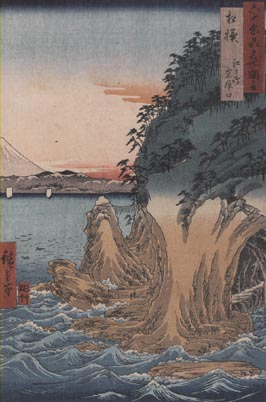
\includegraphics[width=40mm]{vagues.jpg} 
  		\end{minipage}
  	\end{tabular}
  \vspace{0mm}
  \end{frame}
}
}

\usepackage{hyperref}

%%%%%%%%%%%%%%%%%%%%%%%%%%%%%%%%%%%%%%%%%%%%%%%%%%%%%%%%%%%%%%%%%%%%%%%%%%%%%%%%%%%%%%%%%%%%%%%%%%%


\newcommand{\comment}[1]{}


%\makeatletter
%\AtBeginPart{%
 % \beamer@tocsectionnumber=0\relax
  %\setcounter{section}{0}
  %\frame{\partpage}%
%}
%\makeatother


% Pour faire des tables des matières séparées
%\makeatletter
%\numberwithin{section}{part}
%\AtBeginPart{\beamer@tocsectionnumber=\thepart\relax
%}
%\makeatother





\begin{document}


%\begin{frame}
%\titlepage
%\end{frame}
%
%\begin{frame}{Plan du cours}
%\setcounter{tocdepth}{1}
%%\vspace{-10cm}
%\tableofcontents[part=0]
%%\vspace{-4cm}
%\tableofcontents[part=1]
%%\vspace{-4cm}
%\tableofcontents[part=2]
%%\vspace{-4cm}
%\tableofcontents[part=3]
%%\vspace{-4cm}
%\tableofcontents[part=4]
%%\vspace{-4cm}
%\tableofcontents[part=5]
%%\vspace{-4cm}
%\tableofcontents[part=6]
%%\vspace{-4cm}
%\tableofcontents[part=7]
%%\vspace{-4cm}
%\tableofcontents[part=8]
%%\vspace{-4cm}
%\tableofcontents[part=9]
%%\vspace{-4cm}
%
%
%
%\setcounter{tocdepth}{2}
%\end{frame}

%
%%
%\begin{frame}{Organisation du cours :}
%%
%%
%\begin{enumerate}
%\item Introduction -- Analyse dimensionnelle 
%\item Forces dans les fluides au repos -- Hydrostatique
%\item Forces dans les fluides en mouvement 
%\item Cinématique
%\item Equations-bilan -- Régimes d'écoulement
%\item Ecoulements visqueux
%\item Ecoulements inertiels
%\item Ecoulements potentiels et aérodynamique à haut Re
%\item Ecoulements en conduite
%\item Acoustique
%\item Ecoulements compressibles
%\item Ondes de choc
%
%\end{enumerate}
%
%\end{frame}

%
% !TEX root = NotesDeCours.tex



\begin{frame}

  \color{bleu}

  \begin{flushleft}
    
    \Large
   	\bf
    
    Mécanique des fluides 	
    
  \end{flushleft}
  
  \ligne{3} % remplace: \noindent \thickline{0.5mm}{150}

  \begin{flushright}

    \rm

    \textrm{David} \textsc{Fabre}
    
    \vspace{3mm}
    
    IMFT / UPS
    
    Département de Mécanique
    
david.fabre@imft.fr

  \end{flushright}


  \begin{picture}(110, 30)(10, -20)
    \put(15, -17){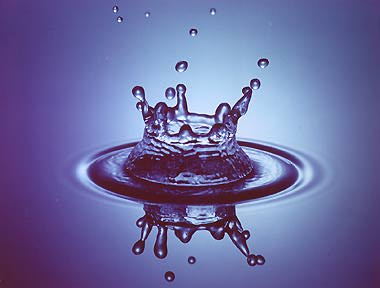
\includegraphics[height=42mm]{./Figures/splash.jpg}}
  \end{picture}

  \vspace{2mm}
  
  \begin{flushright}
    
    \Large
   	\bf
    
    0. Présentation et organisation du cours

  \end{flushright}


\end{frame}


%==================================================================================================
%\part{Présentation du cours}
%==================================================================================================

%--------------------------------------------------------------------------------------------------
\begin{frame}{Objectifs du cours}
%--------------------------------------------------------------------------------------------------

\small

\begin{itemize}
\item[\checkmark]
	Savoir analyser, décrire et caractériser les écoulements 
\item[\checkmark]
	Connaître les phénomènes physiques de base impliqués dans les écoulements
\item[\checkmark]
	Maîtriser la modélisation de ces mécanismes et leur mise en équation : 
\item[] $\rightarrow$ Equation de Navier-Stokes
\item[\checkmark]
	Savoir identifier les mécanismes dominants et ceux qui sont négligeables
\item[]
	$\rightarrow$ définition et exploitation des nombres sans dimension.
\item[\checkmark]
	Savoir simplifier les modèles en conséquence
\item[\checkmark]
	Connaitre les principales techniques de résolution mathématique de ces problèmes
\item[]
	$\rightarrow$ Méthodes locales (résolution exacte de l'équations de NS dans des cas simples) et intégrales (utilisation d'équations-bilan). 
\end{itemize}

\bigskip

\hfill Remarque : liste non exhaustive\ldots

\vspace{20mm}

\end{frame}




%--------------------------------------------------------------------------------------------------
\begin{frame}{Description du module}
%--------------------------------------------------------------------------------------------------

\small


\textbf{Format :} \medskip

\begin{itemize}
\item[\checkmark]
	12 Cours (12x2h) + 12 TD (12x2h) + 3 TPs expérimentaux (3x3h) + 1 TP numérique (3h).
\item[\checkmark]
	Structuration du cours : 1 chapitre = 1 thème par semaine 
	\mytabbing{Structuration du cours :} avec 1 séance de TD associé (2h, la semaine d'après).
	\mytabbing{Structuration du cours :} (NB :  2 cours la première semaine !)
	
\item[\checkmark]
	Entre cours et TD : \textcolor{rouge}{exercice complémentaire} sur Moodle (travail personnel)
	\mytabbing{Entre cours et TD : } Questionnaire Pédagogique Hebdomadaire (sur moodle)
\item[\checkmark]
	TP expérimentaux et numériques : obligatoires, cf. informations sur le tableau d'affichage
\end{itemize}

\pause
\medskip

\textbf{Intervenants :} \medskip

\begin{itemize}
\item
	Cours : David FABRE (david.fabre@imft.fr)
\item
	TD : Mokhtar ZAGZOULE, Frédéric MOULIN
\item
	TP expérimentaux : Frédéric MOULIN
\item
	TP numériques : David FABRE
	
\item ( Enseignants précédents : P. BRANCHER, P. LAURENS, S. SAINTLOS, F. CHARRU... )	
\end{itemize}

\pause
\medskip

\textbf{Evaluation :} \medskip

\begin{enumerate}
\item
	Première session : TP 25\% (num 10\%, expé 15 \%), CC 30\% (exam partiel 2h 25\% + QPH 5\%), CT 45 \% (exam final 3h)  
\item 
	Seconde session : report de la note de TP (20\%), examen terminal 2 (80\%)
\end{enumerate}

\vspace{5mm}

\end{frame}



%--------------------------------------------------------------------------------------------------
\begin{frame}{"Philosophie"}
%--------------------------------------------------------------------------------------------------

\small

Mécanique des fluides = discipline scientifique dont la maîtrise passe par la pratique régulière et
\mytabbing{Mécanique des fluides =} répétée des analyses et des techniques de modélisation et de résolution 
\mytabbing{Mécanique des fluides =} (exercices de TD, développements théoriques et démonstrations du cours)

\bigskip

\qquad $\rightarrow$ \textcolor{rouge}{travail personnel !} \quad (rappel : 1h de présentiel = 1h de travail perso)

\medskip
\qquad $\Rightarrow$ sur les 16 semaines du semestre = en moyenne 3h/semaine minimum (révisions incluses)

\vspace{5mm}
\pause

\textbf{Méthodologie}

\medskip
Entre le cours et le TD : \hfill (NB : pas de rappel de cours en TD\ldots)
\begin{enumerate}
\item relire le cours, 
\item refaire les démonstrations,
\item refaire les exercices traités en cours,
\item travailler l'exercice complémentaire de la semaine.
\item répondre au questionnaire pédagogique hebdomadaire sur moodle !
\end{enumerate}

\vspace{5mm}
\pause

\textsl{Important} : rien n'est complètement trivial, il faut \textcolor{rouge}{se} poser des questions 
$\rightarrow$ \textcolor{rouge}{posez des questions !}

\medskip
Présupposé : il n'existe (presque) pas de question stupide en mécanique des fluides\ldots

\vspace{10mm}

\end{frame}

%--------------------------------------------------------------------------------------------------
\begin{frame}{Informations}
%--------------------------------------------------------------------------------------------------

\small

Quelques informations disponibles sur le tableau d'affichage du L3

\medskip

Plus d'informations sur la page Moodle du cours : %\quad \texttt{\color{rouge} http://moodle.ups-tlse} 
{\tiny \url https://moodle.univ-tlse3.fr/course/view.php?id=1025}

%\medskip

%\qquad $\rightarrow$ puis taper dans \texttt{Recherche} : mécanique des fluides

%\medskip


\pause

\bigskip

Plusieurs documents pédagogiques ou administratifs mis en ligne :

\begin{itemize}
\item
	Résumés de cours
\item
	Compléments de cours (Formulaire,...)
\item
	Enoncés de TD
\item
	\textcolor{rouge}{Exercices complémentaires} (énoncés et corrigés)
\item
	\textcolor{rouge}{Questionnaire Pédagogique Hebdomadaire}
\item
	Enoncés et corrections d'autres exercices et problèmes 
\item
	Programmes informatiques
\item 
	Examens et corrigés 
\item 
	$[\ldots]$
\end{itemize}

\vspace{5mm}

\end{frame}


%--------------------------------------------------------------------------------------------------
\begin{frame}{Pré-requis et références bibliographiques}
%--------------------------------------------------------------------------------------------------

\small
\textbf{Pré-requis :} \smallskip

\begin{itemize}
\item
	Cours de \textcolor{rouge}{Mécanique des milieux continus} (MMC) du premier semestre
\item
	Cours de Thermodynamique du premier semestre
\item
	Notions de mécanique du point, des solides rigides et des systèmes.

	
	
\item
	Outils mathématiques : analyse, algèbre linéaire, géométrie différentielle, 
	\mytabbing{Outils mathématiques :} équations différentielles, intégrales multiples, \ldots
	
	\item 	
	Premières notions de mécanique des fluides ; Cours L2 (M. Marcoux).
	
	Nombreux documents sur moodle :  
	
	{\tiny \url{https://moodle.univ-tlse3.fr/course/view.php?id=1797}}

	
\end{itemize}



\pause

\medskip
\textbf{Modules "compagnons" du second semestre :} \smallskip

\begin{itemize}
\item
	Transferts thermiques 
\item
	Mécanique des solides 
\end{itemize}

\pause

\medskip
\textbf{Références :} \smallskip

\begin{itemize}
\item[] \hspace{-5mm}
	Guyon, Hulin \& Petit : \textsl{Hydrodynamique physique}.
		CNRS éditions, 2001.
%\item[] \hspace{-5mm}
%	Guyon, Hulin \& Petit : 
%		\textsl{Ce que disent les fluides}.	Belin, 2005. 
\item[] \hspace{-5mm}
	Chassaing : \textsl{Mécanique des fluides : éléments d'un premier parcours}.
		Editions Cépaduès, 2000.
\item[] \hspace{-5mm}
	Candel : \textsl{Mécanique des fluides}. 
		Dunod, 2005 (3e édition).
\item[] \hspace{-5mm}
	Darrozès \& François : \textsl{ Mécanique des fluides}.
		Editions de l'ENSTA, 1998.		
		
%\item[] \hspace{-5mm}
%	Ryhming : \textsl{Dynamique des fluides}.
%		Presses Polytechniques et Universitaires Romandes, 2004.
%\item[] \hspace{-5mm}
%	Acheson : \textsl{Elementary Fluid Dynamics}. 
%		Oxford University Press, 1990.
\end{itemize}

\end{frame}

%--------------------------------------------------------------------------------------------------
\begin{frame}{Plan du cours}
%--------------------------------------------------------------------------------------------------

\small

\begin{enumerate}
\item
  Introduction -- Analyse dimensionnelle
\item
  Hydrostatique -- Forces dans les fluides au repos
  \item
  Cinématique -- Description du mouvement d'un fluide.
\item 
  Viscosité -- Forces dans les fluides en mouvement
\item
  Equations de la mécanique des fluides -- régimes d'écoulement
\item
  Ecoulements visqueux
\smallskip
\item[] \qquad $\rightarrow$ partiel
\smallskip
\item
  Ecoulements inertiels
\item
  Ecoulements potentiels
\item
  Ecoulements en conduite
\item
  Acoustique
\item
  Ecoulements compressibles
\item
  Ondes de choc
\smallskip
\item[] \qquad $\rightarrow$ examen terminal
\end{enumerate}

\vspace{5mm}

\end{frame}



%
% !TEX root = NotesDeCours.tex

%\setcounter{section}{0}

%\part{Introduction -- Analyse dimensionnelle}
\nohandout{\section{Introduction -- Analyse dimensionnelle}}

% ================================================================================================ 
% Page de titre :
% ================================================================================================

\begin{frame}

  \color{bleu}

  \begin{flushleft}
    
    \Large
   	\bf
    
    Mécanique des fluides 

  \end{flushleft}
  
  \ligne{3} % remplace: \noindent \thickline{0.5mm}{150}

  \begin{flushright}

    \rm

    \textrm{David} \textsc{Fabre}
    
    \vspace{3mm}
    
    IMFT / UPS
    
    Département de Mécanique
    
  %  brancher@imft.fr

  \end{flushright}

%\begin{picture}(110, 22)(-9, 5)
 % \put( 0, 25){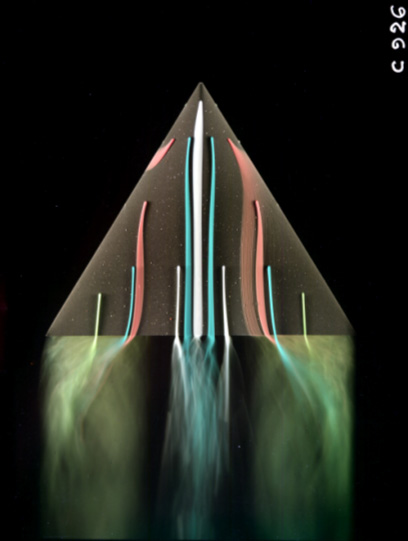
\includegraphics[width=30mm]{./Figures/Werle_aileDelta.jpeg}}
 % \put( 6,  0){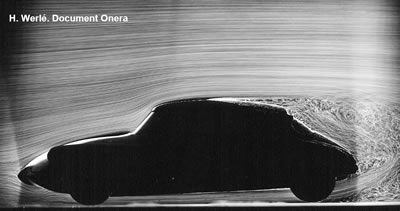
\includegraphics[width=40mm]{./Figures/Werle_Voiture.jpeg}}
  %\put( 0, 23){\color{gris} \small \rm Lignes d'émission dans le sillage d'une maquette d'avion de %type "aile delta" } 
 % \put( 0, 20){\color{gris} \small \rm }
 % \put( 0,  -3){\color{gris} \small \rm Ecoulement dans le sillage d'une maquette d'automobile}
 % \put( 0, -6){\color{gris} \small \rm }
%\end{picture}

\begin{tabular}{cc}
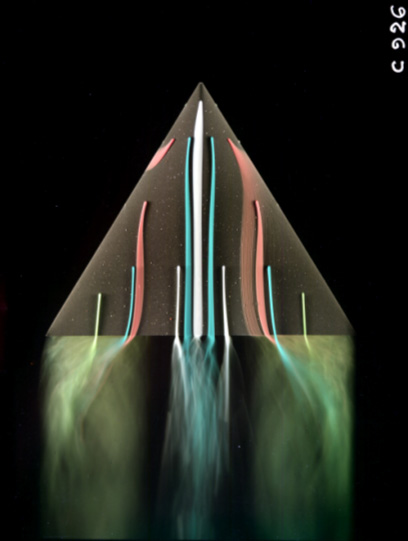
\includegraphics[width=20mm]{./Figures/Werle_aileDelta.jpeg}
&
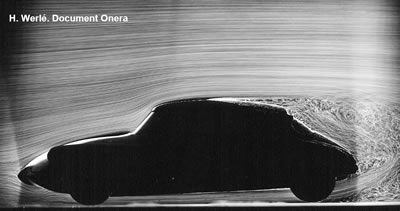
\includegraphics[width=40mm]{./Figures/Werle_Voiture.jpeg}
\\
\small Lignes d'émission dans le sillage  
&
\small Ecoulement dans le sillage 
\\
\small d'une maquette d'avion de type "aile delta"
&
\small d'une maquette d'automobile
\end{tabular}

\medskip
{\small \color{gray}
Images : expériences en tunnel hydrodynamique, H. Werlé (ONERA)
}

  \vspace{12mm}
  
  \begin{flushright}
    
    \Large
   	\bf
    
    1. Introduction -- Analyse dimensionnelle

  \end{flushright}

\end{frame}

%%%%%%%%%%%%%%%%%%%%%%%%%%%%%%%%%%%%%%%%%%%%%%%%%%%%%%%%%%%%%%%%%%%%%%%%%%%%%%%%%%%%%%%%%%
% Sommaire :
%%%%%%%%%%%%%%%%%%%%%%%%%%%%%%%%%%%%%%%%%%%%%%%%%%%%%%%%%%%%%%%%%%%%%%%%%%%%%%%%%%%%%%%%%%


\begin{frame}{Sommaire}

\small
  
\hspace*{2mm}
\begin{tabular}{cc}
		%&
  		\begin{minipage}{62mm}
  			\tableofcontents[firstsection=0]
      \vspace{15mm}
  		\end{minipage}
  		&   
  		\begin{minipage}{60cm}
		  \vspace*{-5mm}  
  			%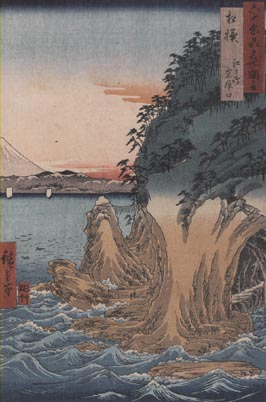
\includegraphics[width=40mm]{vagues.jpg} 
  		\end{minipage}
  	\end{tabular}

\vspace{0mm}

\end{frame}






%==================================================================================================
\subsection{Introduction : Qu'est-ce qu'un fluide ?}
%==================================================================================================

%--------------------------------------------------------------------------------------------------
\begin{frame}{Le millieu fluide : définition \ldots}
%--------------------------------------------------------------------------------------------------

\small

\textbf{Point de vue du thermodynamicien :} \bigskip

Pour un corps pur on appelle phases fluides les deux états fondamentaux suivants : 

\pause

\medskip

\begin{itemize}[<+-| alert@+>]
\item
	gaz (vapeur) : \textrm{O$_2$}, \textrm{CO$_2$}, \textrm{He}, etc.
\item
	liquide : \textrm{H$_2$O}, métaux liquides (\textrm{Hg} à température ambiante, 
	\textrm{Zn} pour $T>450^o C$, \\
	\textrm{Fe} liquide comme dans le noyau liquide de la Terre, ... )
	%dont les mouvements par effet dynamo %sont à l'origine du champ magnétique terrestre)

\item Plus deux états qui ne sont pas des phases bien définies :
	
$\rightarrow$ 
Fluides supercritiques. 
	
$\rightarrow$
	Plasmas (gaz composé d'ions et d'électrons) : 
	haute atmosphère, étoiles (estimation : 99\% de la matière de l'Univers)

\end{itemize}


\pause


\textbf{Point de vue du mécanicien :} \bigskip

Fluide = tout matériau susceptible de s'écouler ; cad de se déformer continument sous l'effet de forces extérieures.


%\medskip

%\textbf{Point de vue du chimiste :} \bigskip

\textbf{
De ce point de vue un fluide être un mélange de corps purs (fluides ou non) :}

\pause

\medskip

\begin{itemize}[<+-| alert@+>]
\item
	mélange de gaz (ex. air : mélange oxygène et azote principalement)

\item mélange de liquides miscibles	
	( pastis = eau+alcool,...) ou solutions (eau de mer, perrier...)

\item Mélanges de liquides non miscibles (ex. eau et huile, vinaigrette)

\item Suspensions (lait, etc...)

\item Collection de corps célestes (anneaux de saturne, galaxies,...)
	
\end{itemize}

%\vspace{15mm}

\end{frame}



\subsection{Modélisation d'un fluide}

\subsubsection{Hypothèse des milieux continus}


%--------------------------------------------------------------------------------------------------
\begin{frame}{Hypothèse des milieux continus}
%--------------------------------------------------------------------------------------------------

\small

Point de vue microscopique (échelle microscopique $\ell$) : 

Description individuelle du mouvement des particules (masse $m_i$, vitesse $\vec{v}_i(t)$).


\smallskip 
\pause

Point de vue macroscopique (échelle macroscopique L) : 

Description globale par des "champs continus" $\rho(\vec x,t)$, $\vec u(\vec x,t)$, ...


\smallskip 
\pause

Ce point de vue est justifié s'il existe un volume élémentaire représentatif (VER) de dimension $L_{VER}$, 
suffisamment grand pour pouvoir faire des statistiques, suffisamment petit pour pouvoir supposer la distribution de particules comme localement homogène.   

$$
\ell \ll L_{VER} \ll L  \quad \longleftrightarrow \quad K_n = \frac{\ell}{L} \ll 1 \quad \mbox{ (Nombre de Knudssen) }
$$

\smallskip 

\pause 

Sous cette hypothèse on peut définir les champs de masse volumique, vitesse, énergie interne massique et température :

$$
\rho = \frac{1}{VER} \sum_{i \in VER} m_i  ,
$$

$$
\vec{u} = \frac{1}{N} \sum_{i \in VER} \vec{v}_i  ,
$$


$$
e = \frac{1}{VER} \left(  \sum_{i \in VER} \frac{ m_i | \vec{v_i} - \vec{u} |^2}{2}  \mbox{ (+ autres formes d'énergie micro.) } \right) , 
$$


$$
T = \frac{ m_p v_q^2}{3 k_b}  \mbox{ avec } v_q^2  =  \frac{1}{N} \sum_{i \in VER} \frac{| \vec{v_i} - \vec{u}|^2}{2} \quad \mbox{(vitesse quadratique moyenne)}
$$
{\tiny 
(pour des particules de masse identique $m_i = m_p$; $k_B = 1.38 \cdot  10^{-23} m^2 kg s^{-2} K^{-1}$  constante de Boltzmann)
}

\pause
Remarque : dans un gaz $\ell$ =  libre parcours moyen $\approx 100 nm$ ; dans un liquide   $\ell$ =  distance intermoléculaire $\approx 0.1 nm$ 

\end{frame}


\subsubsection{Rappels de thermodynamique}

%--------------------------------------------------------------------------------------------------
\begin{frame}{Rappels de thermo}
%--------------------------------------------------------------------------------------------------

\small 


 A l'échelle du VER, la matière est localement homogène, on peut donc faire l'hypothèse de l'équilibre thermodynamique local 
 et utiliser les lois d'état thermodynamiques :
  
  \pause
\medskip
 
\begin{itemize}
\item[$(a)$]  "Equation d'état mécanique"   

%\pause
Formalisme thermo : ${\cal F}( P,T,V,N) = 0$ ($P$ = Pression, cf. chapitre 2) 

%\pause
En mécanique des fluides on utilise généralement cette équation sous la forme $\rho = \rho(P,T)$.

%\pause
Rappels de thermo : compressibilité et dilatabilité.

Echelle de vitesse caractérisant la compressibilité : $c = \sqrt{ \left( \frac{\partial P}{\partial \rho} \right)_S }$

%\pause
Modèles simples :

 - Gaz parfait $\rho = \frac{P}{r T} ; \qquad c = \sqrt{\gamma r T}$
 
- Liquide incompressible : $\rho = \rho_0 (1+\alpha (T-T_0)) ; \qquad c = \infty$

- Liquide incompressible, indilatable :  $\rho = \rho_0 ; c = \infty $

 
	

\pause
\medskip

\item[$(b)$] "Loi d'état énergétique" 

%\pause
Formalisme thermo : $E = E(S,V,N)$ (autres choix possibles, transformations de Legendre, etc...)

%\pause
En mécanique des fluides, on l'utilise généralement sous la forme $e = e(T,P)$ ou $h = h(T,P)$ 

($h = e + P/\rho$ enthalpie massique).
%\pause
Modèles simples :

- Gaz parfaits mono et diatomique : $e = \frac{3 r T}{2}  ; e = \frac{5 r T}{2} $

- Liquide :  $e = e_0 + c_v (T-T_0)$



\end{itemize}

%Remarques : 

%$N$ quantité de matière comptée en moles, en nombre de particules, ou en masse (notée $m$).

%Pour un {\em mélange } on a $N = \sum_{\mbox{espèces}} N_i$, on rajoutera donc des variables intensives supplémentaires : $C_i = N_i/N$ , concentration molaire de l'espèce $i$.

\end{frame}


\subsubsection{Lois de comportement}

\begin{frame}{Lois de comportement}

En plus des lois d'état thermodynamique, il est nécessaire de se donner des lois de comportement:

\begin{itemize}
\item[$(a)$]  Loi de comportement mécanique :

Loi reliant les efforts internes aux déformations du matériau.
\smallskip \pause 

Formalisme MMC :  $\mytensor{\tau} = {\cal F}  ( \mytensor{ D} )$ $ \quad$ (cf. cours MMC et  Chapitre 4.)

\smallskip \pause 

Modèle classique : fluide Newtonien 

 $\mytensor{\tau} = 2 \mu \mytensor{D} $

$ \mu$ : Viscosité dynamique. $[\mu] = Pa. s$.

(autre définition possible : $ \nu$ : Viscosité cinématique. $[\nu] = m^2 /s$.)

\item[$(b)$]  Loi de comportement thermique :

Loi reliant $\vec q$ (flux de chaleur) à la distribution de $T$.

\smallskip \pause 

Modèle classique : loi de Fourrier $\vec q = - \lambda \gradient T$ (cf. cours transferts thermique).

\end{itemize}


\end{frame}

\subsubsection{Synthèse}
\begin{frame}{Synthèse}  
\small

$$
\underbrace{\mbox{Lois d'état}}_{\mbox{ (chap. 2)}}  + \underbrace{\mbox{Lois de comportement}}_{\mbox{ (chap. 4)}} + 
\underbrace{\mbox{Elements de cinématique}}_{\mbox{ (chap. 3)}} 
\rightarrow \underbrace{\mbox{Equations de Navier-Stokes}}_{\mbox{ (chap. 5)}}
$$

\medskip \pause 

Navier-Stokes : EDP non linéaires, structure mathématique compliquée. 

(l'existence de solutions à cette équation dans le cas général est un problème à 1 million de dollars !)

\medskip \pause 

Méthodes de résolution :

\pause
- Résolution exacte possible dans des cas très limités.

\pause
- Résolution numérique (M1 - M2 ; TP numérique) 

\pause
- Résolution {\em approchée } souvent possible, guidée par l'{\em analyse dimensionnelle } qui permet de simplifier les équations en ne gardant que les
 termes les plus importants.




\medskip
\pause

L'analyse dimensionnelle permet, par ailleurs, sans même écrire les équations, de "dégrossir" un problème en identifiant les paramètres importants.

\end{frame}


%%%%%%%%%%%%%%%%%%%%%%%%%%%%%%%%%%%%%%%%%%%%%%%%%%%%%%%%%%%%%%%%%%%%%%%%%%%%%%%%%%%%%%%%%%
\subsection{\bfseries Analyse dimensionnelle}
%%%%%%%%%%%%%%%%%%%%%%%%%%%%%%%%%%%%%%%%%%%%%%%%%%%%%%%%%%%%%%%%%%%%%%%%%%%%%%%%%%%%%%%%%%


%-----------------------------------------------------------------------------------------
\subsubsection{Principe}
%-----------------------------------------------------------------------------------------
\begin{frame}{Analyse dimensionnelle}
%-----------------------------------------------------------------------------------------

\small


Théorème "$\Pi$" (ou Théorème De Vashy -Buckingham) :

\pause 
\medskip

Soit une quantité physique $Y$ dépendant de $n$ paramètres physiques $X_i$ ($i=1$ à $n$).

$$
{Y} = {\cal F }(X_1, X_2, X_n)
$$
\pause

Le fait que $Y$ dépend des variables $X_i$ est vrai indépendamment des unités physiques choisies pour exprimer ces quantités. En notant $[Y]$ l'unité de $Y$, et $[X_i]$ l'unité de $X_i$ :

$$
\frac{Y}{[Y]} = \bar{\cal F }( \frac{X_1}{[X_1]}, \frac{X_2}{[X_2]}, ... \frac{X_n}{[X_n]})
$$
\pause

Alors un choix judicieux d'unités "'intrinsèques" au problème permet de montrer que la quantité adimensionnelle $\frac{Y}{[Y]}$ ne dépend que de $n-n_p$ paramètres adimensionnels, où $n_p$ en le nombre d'unités fondamentales apparaissant dans les dimensions physiques du problème (en général en mécanique $n_p = 3$ : Longueur Temps, Masse).

\pause 
\medskip

%Exemples : 

%\medskip 
%\begin{itemize}
%\item Chute d'un objet dans le vide
%\medskip 
%
%\item  Flexion d'une poutre sous l'effet de son poids
 %\end{itemize}
  %\pause 


Remarques (importantes) : 
\begin{itemize}
\item Souvent des {\color{bleu} constatations expérimentales} et/ou des {\color{purple} considérations géométriques} et/ou l'étude de la {\color{red} structure des équations }  permettent de réduire encore plus le nombre de paramètres ou de préciser la dépendance vis-à-vis de ceux-ci. 

\item Si un paramètre sans dimensions est soit très petit, soit très grand, il arrive souvent que la relation devienne indépendante de ce paramètre
(mais ce n'est pas une règle générale ! Il faut toujours rester guidé par l'expérience et/ou l'analyse des équations)

\end{itemize}

{\color{green}(Exemples)} 


\vspace{0mm}

\end{frame}

\begin{frame}{ Exemple 1 : Période d'un pendule} 

\small
(Pendule de longueur $L$,  masse $m$, position angulaire initiale $\theta_0$)
\pause

\begin{itemize}

\item Loi recherchée en fonction des paramètres physiques supposés pertinents :
$$
 T = {\cal F} (L,m,g,\theta_0)
$$

\item  Mise sous forme adimensionnelle de la relation :
$$
\frac{T}{[T]} = \overline{\cal F} \left( \frac{L}{[L]},  \frac{m}{[m]},\frac{g}{[L] \cdot [T]^{-2}} ,\frac{\theta_0}{1} \right)
$$

\item Choix des unités "intrinsèques" au problème :
$$
[L] = L, \quad [m] = m , \quad [T] = \sqrt{L/g}
$$

Ce qui conduit à : 
$$
\frac{T}{\sqrt{L/g}} = \overline{\cal F} \left( 1,  1, 1, \theta_0 \right) \quad \mbox{ soit } T = \sqrt{\frac{L}{g}} f(\theta_0)
$$


\item Simplification : 

Lorsque $\theta_0\ll 1$ la période ne dépend plus de $\theta_0$  ({\color{bleu} Constatation expérimentale}, justifié également par l'{\color{red} étude des équations} )

$$ \longrightarrow T = \sqrt{\frac{L}{g}} \times C_{te} $$


\item Remarque : la solution exacte du problème (exercice niveau L1) est $T = 2 \pi  \sqrt{\frac{L}{g}}$. 
Le résultat prédit par analyse dimensionnelle est bien de cette forme (mais ne donne pas la valeur de la constante).

\end{itemize}


\end{frame}




\begin{frame}{ Exemple 2 : Flexion d'une poutre pesante} 

\small

(Poutre de longueur $L$, épaisseur $e$, largeur $b$, masse $m$, module d'young $E$, coef. de Poisson $\nu$)
\pause

\begin{itemize}

\item Loi recherchée en fonction des paramètres physiques supposés pertinents :
$$
 \delta = {\cal F} (L,e,b,m,g,E,\nu)
$$



\item  Mise sous forme adimensionnelle de la relation :
$$
\frac{\delta}{[L]} = \overline{\cal F} \left( \frac{L}{[L]},   \frac{e}{[L]},  \frac{b}{[L]}, \frac{m}{[m]},\frac{g}{[L] \cdot [T]^{-2}} ,\frac{E}{[m][L]^{-1} [T]^{-2]}} \right)
$$

\item Choix des unités "intrinsèques" au problème :
$$
[L] = L, \quad [m] = m , \quad [T] = \sqrt{L/g}
$$

Ce qui conduit à : 
$$
\frac{\delta}{L} = \overline{\cal F} \left( 1,  \frac{e}{L}, \frac{b}{L}, 1,1,\frac{E L^2}{m g}, \nu  \right) \quad \mbox{ soit }  
\delta = L f \left(  \frac{e}{L}, \frac{b}{L}, \frac{E L^2}{m g}, \nu 
\right)
$$


\item Simplifications : 

\begin{itemize}
\item $\delta$ ne dépend pas de $b$ ( {\color{purple} considération géométrique} ).
\item $\delta$ ne dépend pas de $\nu$ ( {\color{bleu} constatation expérimentale} ; justifié également par l'{\color{red} étude des équations} ).
\item $\delta$ est proportionnel à $m$ ( {\color{bleu} constatation expérimentale} ; justifié également par l'{\color{red} étude des équations} ).
\end{itemize}


$$ 
\longrightarrow \delta  = f(e/L) \times \frac{m g}{E L} 
$$


\item Remarque : la solution exacte du problème (cf. cours Méca solides) est $\delta =  \frac{ 3 m g L^3}{2 E e^4}$ qui est bien de la forme attendue. 


\end{itemize}


\end{frame}







\begin{frame}{Utilisation pratique}

\small
Méthode pratique pour appliquer la méthode d'analyse dimensionnelle :

\bigskip
\begin{itemize}
\item Listez les paramètres physiques {\em pertinents } et {\em indépendants }

\item Listez la dimension physique de toutes les quantités intervenant dans le problème.

\item Ecrire la relation fonctionnelle sous forme adimensionnelle.

\item Faire le choix "judicieux" des unités, et en déduire les paramètres adimensionnels du problème.

\end{itemize}

\bigskip

Remarque : le choix peut être plus ou moins "judicieux", des choix différents amènent à des jeux de paramètres différents, tous équivalents.  
%(mais on peut passer d'un jeu de paramètres à un autre par un simple changement de variable).

\medskip 

Le "bon" choix (guidé par l'expérience) est celui qui fait apparaître les nombres adimensionnels "classiques" (Reynolds, Mach, Froude, Bond, ....).

\medskip 
$=>$ document "Formulaire", Tableau A "Nombres sans dimensions" 

\end{frame}




\subsubsection{Application : force exercée sur un véhicule}

\begin{frame}{Application : forces sur un véhicule}  
%Force exercée sur un objet placé dans un écoulement uniforme}

\small
%
Considérons un objet de dimension $L$ placé dans un écoulement uniforme de vitesse $U$
(ou de manière équivalente un objet se déplaçant à la vitesse $U$ dans un fluide au repos).

\smallskip


On cherche à estimer les composantes $F_x$ et $F_z$ 
de la force exercée par le fluide sur l'objet.

\medskip
\pause

Listons les paramètres physiques pertinents et indépendants :

\medskip
\pause

$$
F_x = {\cal F}( U, L, P_0, \rho_0, \nu, g, {\cal G}_i)
$$

$P_0, \rho_0, \nu$ valeurs "de référence" des propriétés du fluide ;

$g$ accélération du champ de pesanteur ;

${\cal G}_i$ paramètre(s) géométrique(s) sans dimension (exemple : angle d'incidence, rapport de forme, ...)



\medskip
\pause

Par application du théorème "$\Pi$" :

$$
\frac{F_x}{\rho_0 L^2 U^2} = \bar{\cal F} \left( \frac{U L}{\nu}, \frac{U}{\sqrt{gL}} , \frac{P_0}{\rho_0 U^2}, {\cal G}_i \right)
$$


On reconnait les nombres sans dimension : $Re= \frac{U L}{\nu}$, $Fr = \frac{U}{\sqrt{gL}}$

\smallskip
\pause

Par convention on introduit une "surface de référence" $S \approx L^2$, et on pose donc 
 
$$
F_x = \frac{1}{2} \rho_0 S U^2 C_x(Re, Fr, P_0/\rho U^2, {\cal G}_i)
$$

De même pour $F_z$ : 

$$
F_z = \frac{1}{2} \rho_0 S U^2 C_z(Re, Fr, P_0/\rho U^2,{\cal G}_i)
$$

\end{frame}

%==========================================================================================
%\subsubsection{Le modèle de fluide parfait}
%=========================================================================================

%-----------------------------------------------------------------------------------------
\subsubsection{Cas d'un liquide homogène}
%-----------------------------------------------------------------------------------------
\begin{frame}{Cas d'un liquide homogène (bateau, sous-marin)}
%-----------------------------------------------------------------------------------------

\small

Un liquide est incompressible pour des raisons thermodynamiques.

Supposons donc que la masse volumique homogène et vaut $\rho = \rho_0$.


\medskip
\pause 

\begin{itemize} 
\item Première simplification :

L'étude de la structure des équations montre que $P_0$ n'intervient pas dans le problème.

$\rightarrow$  $[C_x,C_z]$ ne dépendent pas de $P_0/\rho_0 U^2$.


\smallskip
\pause 

\item Seconde simplification : 

Si l'objet n'est pas a proximité d'une surface libre (cas d'un sous-marin), on montre  que la force se décompose en deux parties : 

Une composante hydrodynamique qui est solution du problème fluide "non pesant"   

Une composante hydrostatique qui n'est autre que la poussée d'Archimède.
 
% \smallskip
%$$
%{F_x} = \frac{1}{2} \rho_0 S U^2 C_x(Re, {\cal G}_i) ; \quad {F_z} = \frac{1}{2} \rho_0 S U^2 C_z(Re, {\cal G}_i) + \rho_0 V g \myvec{e}_z
%$$

{\color{vert}[Démonstration : chapitre 5]}

\end{itemize}

\pause
\medskip
{\bf Remarque : }

Cette seconde simplification n'est pas valable dans le cas d'un objet traversant une surface libre 
(cas des bateaux)
%(la condition dynamique à la surface libre est la continuité de $p$, pas de $\hat{p}$ !) 
\smallskip
\pause 

Pour un bateau la force de traînée est de la forme :

$$
{F_x} = \frac{1}{2} \rho_0 S U^2 C_x(Re,Fr, {\cal G}_i) 
$$

Dans la plupart des cas l'effet de $Fr$ est dominant  (traînée de vagues).


\end{frame}

\begin{frame}{Cas d'un gaz (avion, automobile)}
%-----------------------------------------------------------------------------------------

\small
Pour un gaz (compressible) :
\smallskip
\pause 
\begin{itemize}


\item L'effet de la gravité est en général négligé.
%(plus rigoureusement, il peut être séparé des effets aérodynamiques et contribue seulement à la poussée d'Archimède).

\pause

\item 
Le paramètre $P_0/\rho_0 U^2$ est directement relié au {\em Nombre de Mach} $Ma$ : 
$$
Ma^2 = \frac{U^2}{c^2} \quad \mbox{ avec } c^2 = \frac{\partial P}{\partial \rho} = \frac{1}{P_0 \chi_s} = \frac{\gamma P_0}{\rho_0}
$$

%\pause 

\end{itemize}

\smallskip
\pause 
Les forces sur un objet en mouvement dans un gaz (par ex. un avion) sont donc données par :

$$
F_x = \frac{1}{2} \rho_0 S U^2 C_x(Re,Ma, {\cal G}_i) 
$$

$$
F_z = \frac{1}{2} \rho_0 S U^2 C_z(Re,Ma, {\cal G}_i) 
$$

\pause
\medskip

On justifiera plus tard que :
\smallskip

\begin{itemize}
\item $c$ est la vitesse des ondes acoustiques (chapitre 10).

\item si $Ma < 0.3$ la structure de l'écoulement (et les forces induites) ne dépend pas du nombre de Mach. 
L'écoulement d'un gaz (compressible) est dans ce cas identique à celui d'un liquide incompresssible.
(on parle alors d'écoulement incompressible ; cf. chap. 5 et 11)
 
 \end{itemize}
 
 
 %On parle de "régime d'écoulement isovolume", ou (par abus de language) "régime d'écoulement incompressible". (En pratique ce régime est justifié si $Ma\lesssim 0.3$).
 
 \pause 
 \medskip
 
{\bf Conséquence :} dans le "régime d'écoulement incompressible" les forces sur un avion (ou sur une automobile) sont de la forme 

$$
[F_x,F_z] = \frac{1}{2} \rho_0 S U^2 [C_x(Re,{\cal G}_i) ,C_z(Re,{\cal G}_i) ] 
$$


\end{frame}




\subsubsection{Lois de similitude}
\begin{frame}{Lois de similitude}

\small

Problème pratique pour un ingénieur : 

Pour un véhicule de longueur $L$, vitesse $U$, dans un fluide et un environnement de caractéristiques ($\rho_0,P_0,\nu,g$), estimez la force de traînée $F_x$ (et/ou la portance $F_z$).

\pause
\medskip

Méthode expérimentale : On dispose d'une maquette à l'échelle réduite 
$L_m$,  vitesse $U_m$, {\em Géométriquement similaire} (c.a.d. les paramètres ${\cal G}_i$ sont les mêmes que pour le véhicule). 

On effectue une expérience dans un environnement de caractéristiques ($\rho_m,P_m,\nu_m,g_m$).

\smallskip

On mesure une force $F_{x,m}$ sur la maquette. 
\smallskip

Comment en déduire la force $F_x$ sur le véhicule à échelle réelle ???

\pause
\medskip


{\bf Principe de similitude :} 
Si les paramètres sans dimensions sont les mêmes dans les conditions réelles et celles de l'expérience (conditions de {\em similitude}), alors le coefficient de force sans dimension $C_x$ prend la même valeur !

\pause
\medskip

Exemples d'application :
\begin{itemize}

\item Cas d'une automobile : Un seul paramètre $Re$. 

On peut donc être en similitude exacte. (N.B. le fluide dans l'expérience peut être différent de l'air...)

\item Cas d'un avion : Deux paramètres $Re, Ma$. 

Impossibilité d'être en similitude exacte (a moins de faire varier fortement la température...)

\item Cas d'un bateau :  Deux paramètres $Re, Fr$. 

Impossibilité d'être en similitude exacte (a moins de faire l'expérience sur une autre planète...)

\end{itemize}


\pause
\medskip

Dans les deux derniers cas, en pratique, on se met en {\em similitude partielle } en privilégiant le paramètre le plus important (respectivement $Ma$ et $Fr$), et on corrige l'effet du nombre de $Re$ par des méthodes semi-empiriques issues de la modélisation des effets visqueux.

\end{frame}



\comment{
%--------------------------------------------------------------------------------------------------
\begin{frame}{Protocole de modélisation}
%--------------------------------------------------------------------------------------------------

\small

Objectif : décrire et comprendre pour prédire voire contrôler les écoulements de fluides

\medskip 

\centerline{$\rightarrow$ \sc modélisation}

\bigskip

\pause

Méthode : 

\medskip

\begin{enumerate}
\item
	\textcolor{rouge}{mise en équation} à partir 
  \begin{itemize}
	\item[\checkmark]
		des principes de conservation de la physique (équations de bilan)
	\item[\checkmark]
  		des \textcolor{rouge}{équations d'état}, issues de modèles microscopiques, 
		de principes de la thermodynamique, ou de considérations empiriques
		\\ (cf. suite de ce cours)
	\item[\checkmark] des \textcolor{rouge}{lois de comportement} (loi rhéologique, lois de diffusion massique et thermique, etc...) 
		également obtenues a partir de {\em modèles microscopiques} 
		ou de manière {\em empirique}
		\\ (cf. cours 2 et 4)
	\end{itemize}
\item[]
  $\rightarrow$ système d'équations complexes (EDP non linéaires, \ldots)
\pause
\bigskip
\item
	\textcolor{rouge}{résolution} numérique discrétisée (simulation sur ordinateur)
  ou analytique approchée :
	\begin{enumerate}
	\item[(a)]
		mise en évidence de paramètres sans dimension caractéristiques des phénomènes physiques en présence
	\item[(b)]
  		simplification asymptotique des équations d'origine dans la limite de nombres sans dimension 
  		très petits (ou très grands).
	\end{enumerate}
\end{enumerate}

\vspace{20mm}

\end{frame}






\subsection{Compléments : rappels de thermo}


%--------------------------------------------------------------------------------------------------
\begin{frame}{Equations d'état : cas du gaz parfait}


Echelles de longueurs microscopiques dans un gaz :

- Echelle moléculaire $a \approx 0.1 nm$

- Distance intermoléculaire moyenne $d \approx (V/N)^{1/3} \approx 3 nm$

- Libre parcours moyen $\ell \approx d^3 / a^2  \approx 100 nm$ 


\begin{itemize}
\item 
$T$ est une mesure de l'agitation microscopique :

$$
 \frac{m v_q^2}{2} = \frac{3 k_b T}{2}
$$

(ordre de grandeur : $v_q \approx 100 m/s$). 

\item 
$P$ est la force surfacique due aux collisions.

\end{itemize}

%\medsip
%$\rightarrow$ 

Equation d'état mécanique : $PV =  NRT$.
 
 (Démo microscopique :  $P \approx (N/V) v_q^2 \equiv NRT/V$).
 
 \medskip

Ou en variables intensives :

$P = \rho r T$.

 
% \bigskip Equation d'état énergétique :
 
% $H = C_p T$ 
  
% $C_p = 7 NR/2$ pour un gaz parfait diatomique.
 
\end{frame}

%--------------------------------------------------------------------------------------------------
\begin{frame}{Equations d'état : cas des liquides}

\small 
Etat beaucoup plus dense : distance intermoléculaire moyenne $d \approx a \approx 0.1 nm$

\medskip 
Contrairement au gaz un liquide a un {\em volume propre} $V_0$ correspondant à une énergie interne minimale (pour lequel les interactions moléculaires sont équilibrées ; attractions $\approx$ répulsions )

\medskip

Il faut exercer une très grande force (pression) pour faire varier le volume (et donc augmenter l'énergie interne).

\begin{tabular}{ll}
\begin{minipage}{.5\textwidth}
$ P = -\frac{\partial U}{\partial V}_S $
\end{minipage}
&
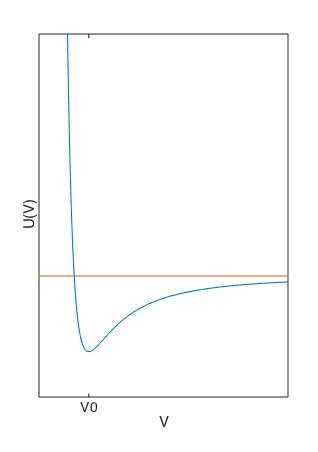
\includegraphics[width=0.2\linewidth]{Figures/UV_liquide.jpg}

\end{tabular}

\smallskip 
- Si $V<V_0$ , $P>0$ (liquide comprimé)

\smallskip
- Si $V>V_0$ , $P<0$ (liquide en dépression ; état métastable mais parfois observé !)

\medskip 


Le coefficient 
$ \chi_S = 1/V {\left.\partial V/\partial P\right|}_S \equiv  1/V \left( {\left.\partial^2 U/\partial V^2\right|}_S \right)^{-1}$ 
est très faible : les liquides sont très peu compressibles.

\medskip

Donc l'équation d'état est souvent dégénérée en  $V = V_0$.

%\qquad

%Equation d'état énergétique :

%$

\medskip

Ou en variables intensives : $\rho = \rho_0$.

\medskip



Remarque : $\rho_0$ peut dépendre de $T$, on parle alors de liquide incompressible dilatable.


\bigskip

%--------------------------------------------------------------------------------------------------
\begin{frame}{Hypothèse de l'équilibre thermodynamique local}
%--------------------------------------------------------------------------------------------------


Les lois d'état issues de la thermodynamiques sont valables dans les conditions de l'équilibre 
(repos, P T uniformes, pas de force extérieure).

\medskip


Peut-on les utiliser pour décrire l'état local d'un fluide aux propriétés non uniforme et éventuellement en mouvement ?

\medskip 

Hypothèse de l'équilibre thermodynamique local : 

\medskip

Avec l'approche du Milieu Continu on suppose les propriétés localement homogènes à l'échelle
d'un Volume Elémentaire Représentatif de dimension grande devant l'échelles microscopiques 
$\ell$ et petite devant l'échelle macroscopique $L$ .

\medskip 
Cette approche est justifiée sous la condition :

\smallskip
$\Knudsen \equiv \ell / L \ll 1 $

\smallskip

$\Knudsen$ est le Nombre de \textcolor{rouge}{\bf Knudsen} (nombre sans dimension).




%\smallskip

%\hfill [$\rightarrow$ cf. expérience de mesure de la masse volumique$^\star$]

%\medskip

%Cette échelle de longueur définit l'échelle de la \textcolor{rouge}{particule fluide},  
%sur laquelle \\ la matière est dans un état local homogène ($a\ll L$).

% de quasi-équilibre thermodynamique, 
%\\
%c'est-à-dire assez grande ($a \gg \ell$) pour contenir suffisamment d'atomes ou de molécules 
%\\
%pour que cette notion de quasi-équilibre ait un sens du point de vue de la physique statistique.

\vspace{5mm}

\end{frame}





%\vspace{10mm}

\end{frame}


%
%%--------------------------------------------------------------------------------------------------
%\begin{frame}{Motivations : des défis scientifiques actuels}
%%--------------------------------------------------------------------------------------------------
%
%\small
%
%Les fluides interviennent dans de nombreuses applications et sont au c{\oe}ur d'enjeux économiques 
%et écologiques majeurs.
%
%\medskip
%
%Ils sont aussi sources de plusieurs verrous scientifiques fondamentaux, qui les associent 
%aux plus grands défis de la physique moderne, comme en témoigne le classement effectué 
%par le CNRS à l'occasion de l'année mondiale de la physique par l'ONU en 2005 :
%
%\medskip
%
%\begin{itemize}
%\item \textcolor{vert}{Les mystères de l'eau}
%\item \textcolor{rouge}{Insaisissable turbulence}
%\item \textcolor{vert}{L'obscure nature du verre}
%\item \textcolor{rouge}{Les ambiguïtés des solides liquides}
%\item Les états étranges de la matière
%\item Les frontières incertaines du monde quantique
%\item Antimatière o{\`u} es-tu ?
%\item Energie noire, la grande inconnue
%\item Le casse-tête de l'unification des forces
%\item A la poursuite des particules élémentaires
%\end{itemize}
%
%\end{frame}



%
%%==================================================================================================
%\subsubsection{Motivations}
%%==================================================================================================
%
%%--------------------------------------------------------------------------------------------------
%\begin{frame}{Motivations : des applications multiples}
%%--------------------------------------------------------------------------------------------------
%
%\small
%
%\vspace{5mm}
%
%L'intérêt pour l'étude des écoulements des fluides est motivé par de nombreuses applications, \\ entre autres :
%
%\begin{itemize}
%\item<2->
%  Aérodynamique
%\item<3->
%  Hydrodynamique
%\item<4->
%  Bio-ingénierie et systèmes biologiques
%\item<5->
%  Production d'énergie
%\item<6->
%  Géologie
%\item<7->
%  Hydraulique et hydrologie
%\item<8->
%  Météorologie
%\item<9->
%  Planétologie, astrophysique
%\item<10->
%	Gestion des ressources en eau
%\end{itemize}
%
%\begin{overprint}
%
%  \onslide<2>   
%  \begin{center}
%    \begin{picture}(45, 40)
%    \put(0, 5){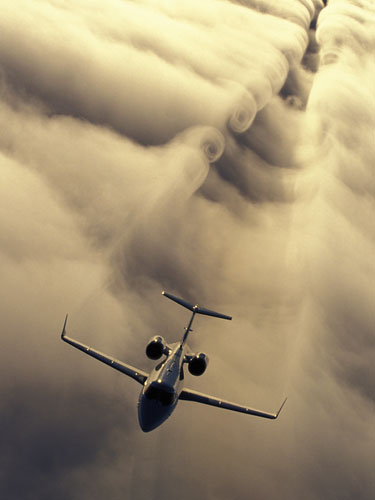
\includegraphics[width=45mm]{trailing_vortices_railtrack.jpg}}
%    \end{picture}
%  \end{center}
%
%  \onslide<3>   
%  \begin{center}
%    \begin{picture}(90, 40)
%    \put(0, 5){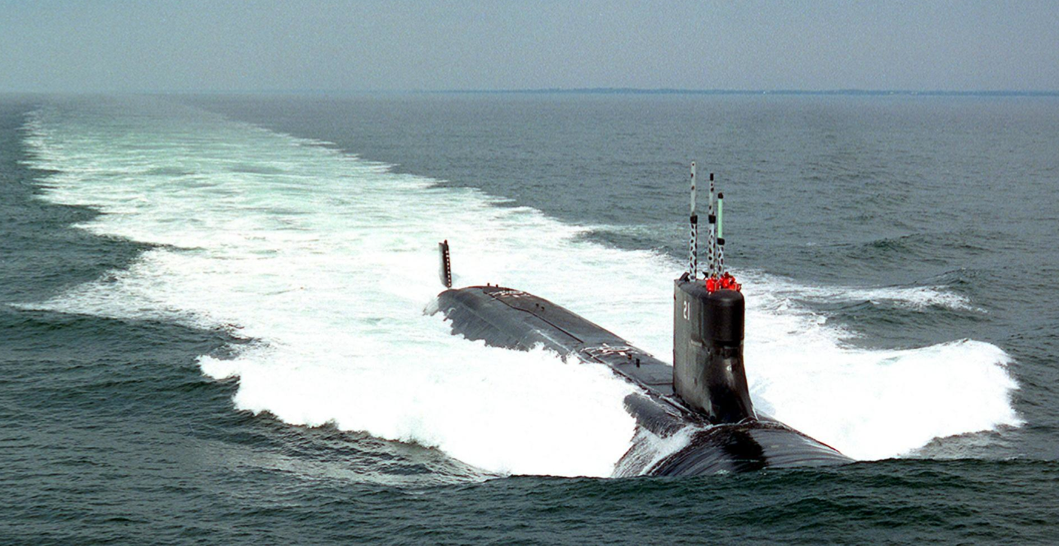
\includegraphics[width=90mm]{sous_marin.png}}
%    \end{picture}
%  \end{center}
%
%  \onslide<4>   
%  \begin{center}
%    \begin{picture}(100, 40)
%    \put(0, 5){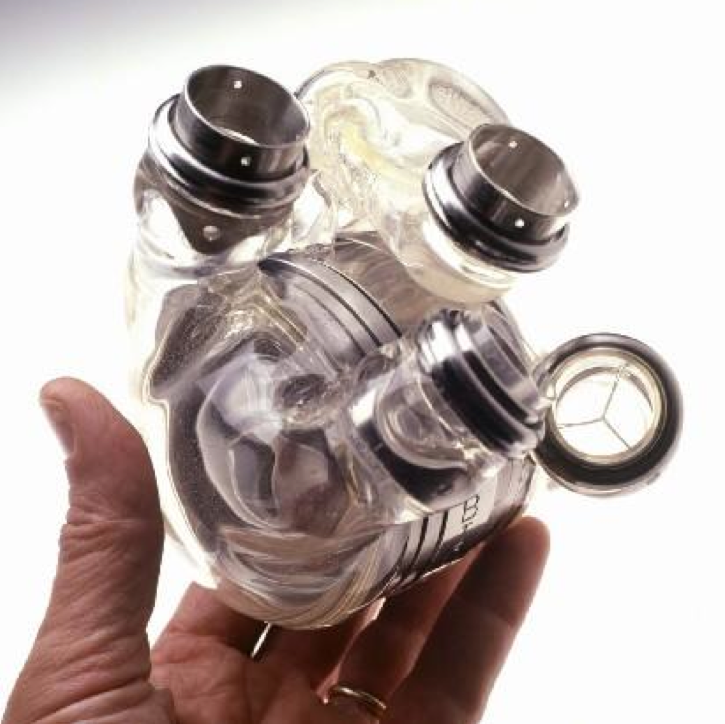
\includegraphics[width=45mm]{coeur_artificiel.png}}
%    \put(50, 5){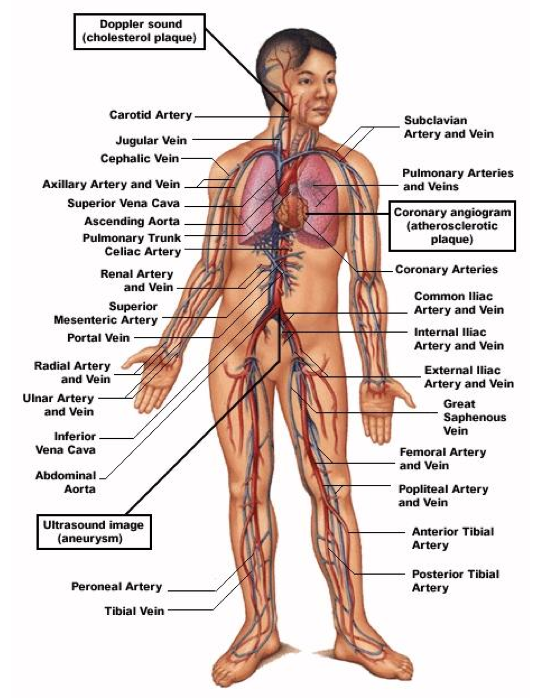
\includegraphics[width=50mm]{circulation_sang.png}}
%    \end{picture}
%  \end{center}
%
%  \onslide<5>   
%  \begin{center}
%    \begin{picture}(60, 40)
%    \put(0, 5){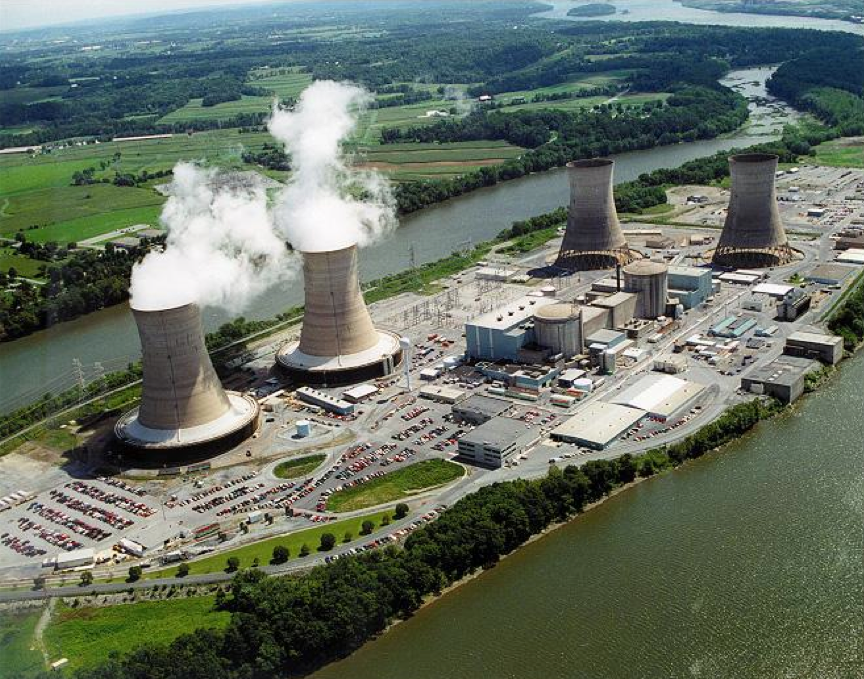
\includegraphics[width=60mm]{centrale_nucleaire.png}}
%    \end{picture}
%  \end{center}
%
%  \onslide<6>   
%  \begin{center}
%    \begin{picture}(65, 40)
%    \put(0, 5){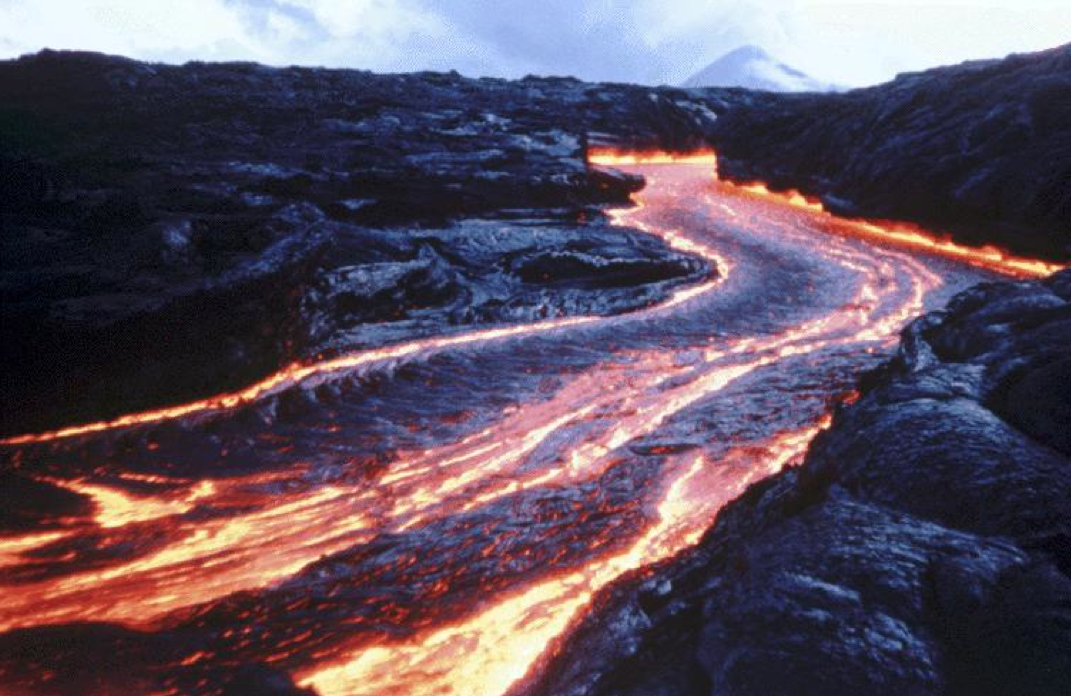
\includegraphics[width=65mm]{coulee_lave.png}}
%    \end{picture}
%  \end{center}
%
%  \onslide<7>   
%  \begin{center}
%    \begin{picture}(105, 40)
%    \put(0, 5){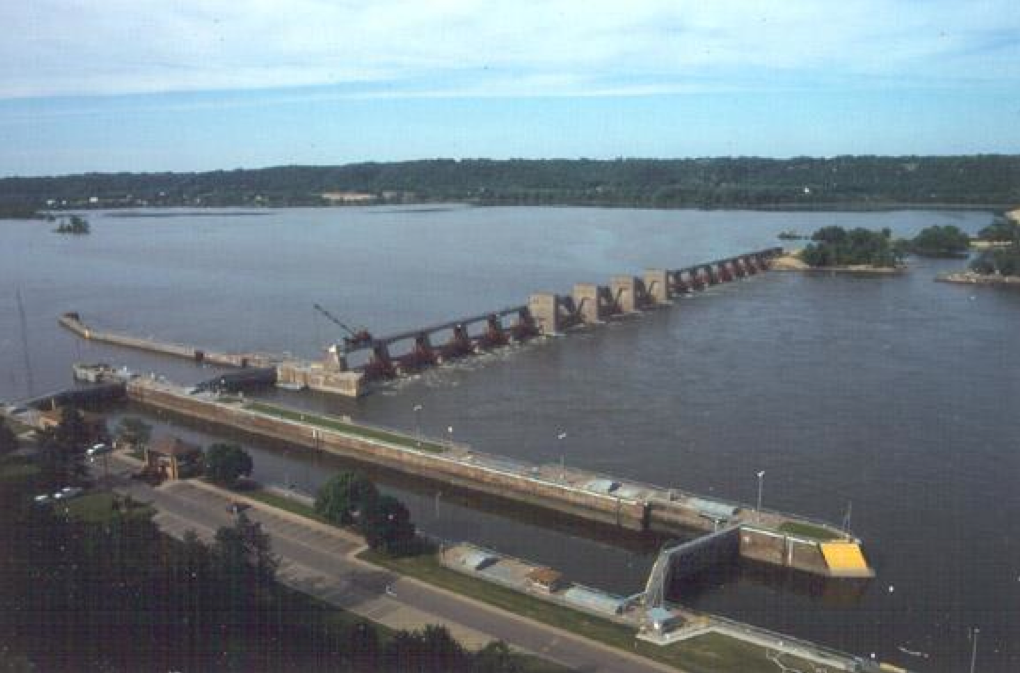
\includegraphics[height=35mm]{barrage_hydraulique.png}}
%    \put(55, 5){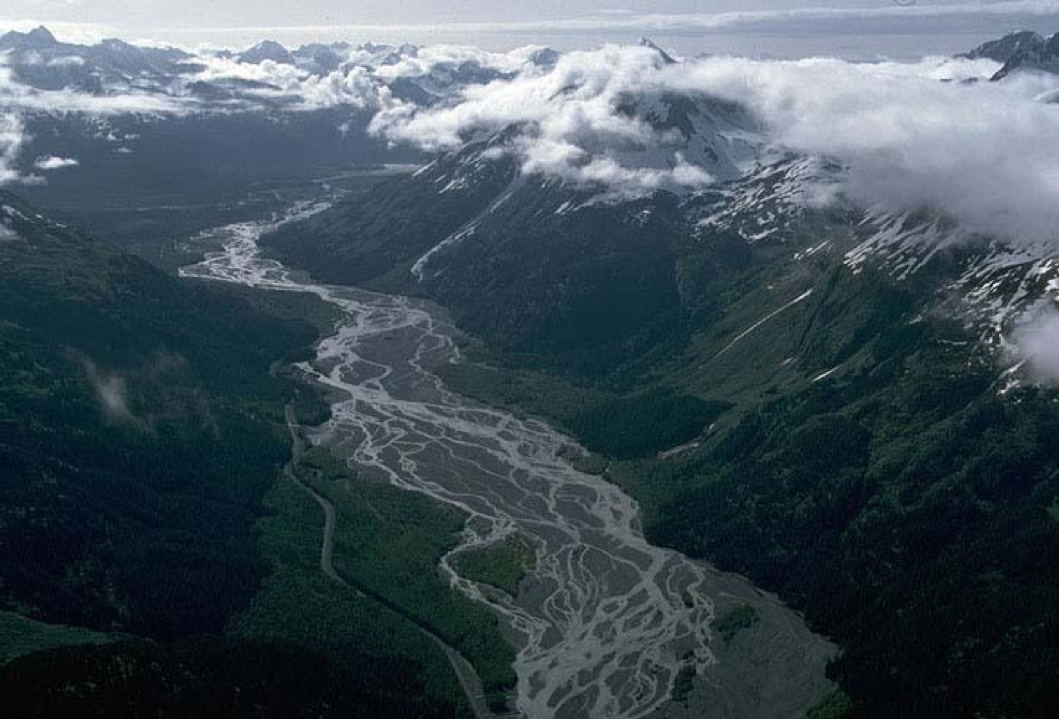
\includegraphics[height=35mm]{bassin_vallee.png}}
%    \end{picture}
%  \end{center}
%
%  \onslide<8>   
%  \begin{center}
%    \begin{picture}(100, 40)
%    \put(0, 5){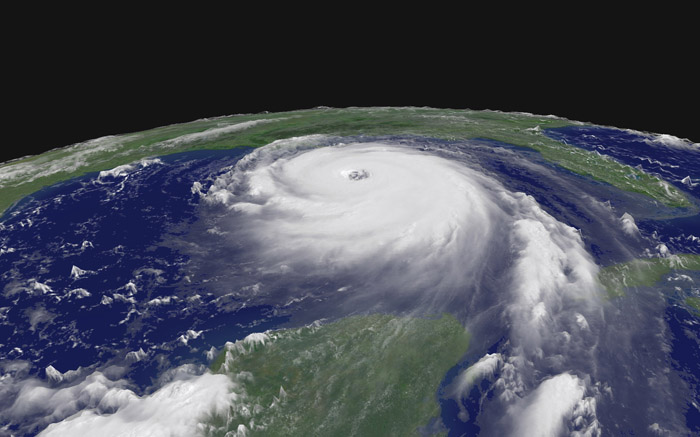
\includegraphics[height=35mm]{katrina_08-28-2005_NOAA.jpg}}
%    \put(58, 5){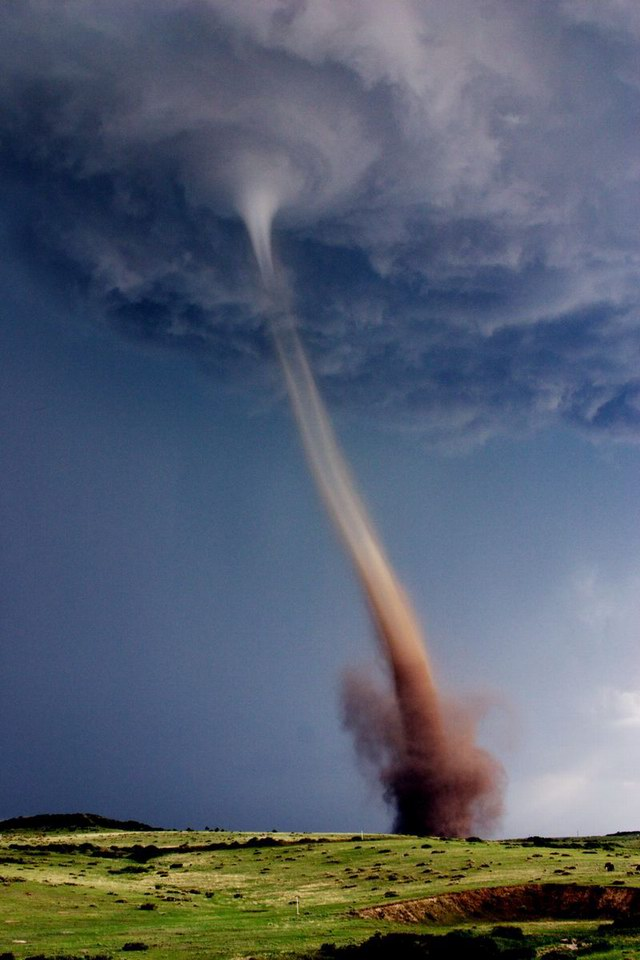
\includegraphics[height=60mm]{tornade.jpg}}
%    \end{picture}
%  \end{center}
%  
%    \onslide<9>   
%  \begin{center}
%    \begin{picture}(100, 40)
% %   \put(0, 5){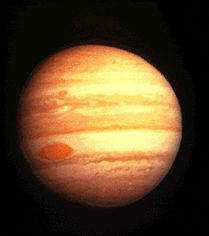
\includegraphics[height=35mm]{Jupiter.jpg}}
%  %  \put(58, 5){\includegraphics[height=60mm]{Galaxie.jpg}}
%    \end{picture}
%  \end{center}
%
%
%  \onslide<10>   
%  \begin{center}
%    \begin{picture}(100, 40)
%    \put(0, 5){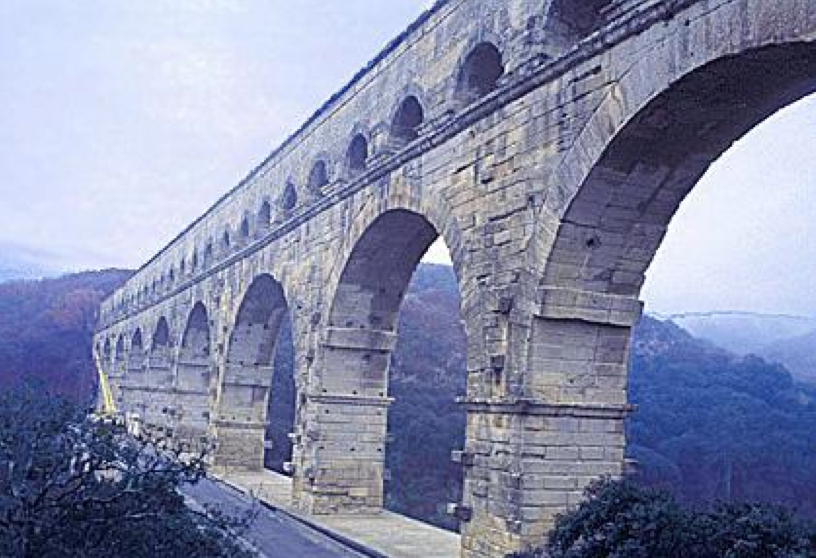
\includegraphics[height=33mm]{aqueduc.png}}
%    \put(50, 4.8){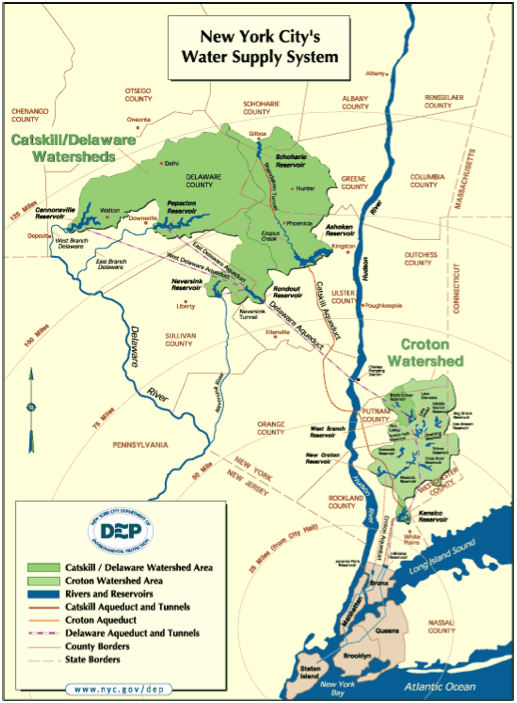
\includegraphics[height=60mm]{reseau_eau_New_York.png}}
%    \end{picture}
%  \end{center}
%
%
%\end{overprint}
%
%\end{frame}

%
%%--------------------------------------------------------------------------------------------------
%\begin{frame}{Des définitions diverses\ldots} 
%%--------------------------------------------------------------------------------------------------
%
%\small
%
%\textbf{Point de vue du physicien :} \bigskip
%
%Certains systèmes constitués d'un grand nombre d'objets solides peuvent avoir un 
%comportement fluide (et être décrits par les outils de la mécanique des fluides) :
%
%\pause
%
%\medskip
%
%\begin{itemize}[<+-| alert@+>]
%\item
%	sable (sablier)
%
%\item
%	trafic automobile, piétons	
%\item
%	galaxies, disques d'accrétion (systèmes solaires en formation)
%\item
%	boues, neige (avalanches), nuages (particules d'eau liquide ou solide)
%%\item
%%	verre ?
%%\item
%%	pâtes agroalimentaires (ketchup, dentifrice, etc.)
%\end{itemize}
%
%\end{frame}


%--------------------------------------------------------------------------------------------------
\begin{frame}{Des définitions diverses\ldots} 
%--------------------------------------------------------------------------------------------------

\small

\textbf{Point de vue du mécanicien :} \bigskip

Mécanique = science qui s'intéresse au lien entre forces et mouvements.

"Un fluide est un matériau qui, sous l'effet d'une contrainte imposée, se déforme continument".

Mais le comportement solide ou fluide peut dépendre :

\medskip

\pause


\textbf{De la valeur de la contrainte exercée :}

\begin{itemize}[<+-| alert@+>]

\item Dentifrice, ketchup,...

\item Neige (avalaches)

\item mousses,...

\end{itemize}

\medskip 

\pause

\textbf{De la durée d'observation :}

\begin{itemize}[<+-| alert@+>]
\item 
	Glacier (glace : eau solide) : 
	vitesse de coulée, %si épaisseur supérieure à 50 m, 
	environ 10 cm à 10 m / jour

\item
	Bitume (goudron) :
	Expérience de l'université de Brisbane, 9 gouttes depuis 1927.
	
\item Verre ?

\item 

	\hyperlink{frame:manteau_terrestre}{manteau terrestre$^\star$}
	(roches solides) : comportement fluide à l'échelle de temps géologique 
	\\ ($\sim$ million d'années) avec des déformations de l'ordre du cm / an 
	(tectonique des plaques de surface), en particulier 
	sous l'effet du phénomène de convection thermique dans le manteau.
% qui se comporte donc comme un fluide compressible (dilatable) !

\item Solution de Maïzena 

Une expérience amusante : 
\href{https://www.youtube.com/watch?v=f2XQ97XHjVw}{
\color{blue}{https://www.youtube.com/watch?v=f2XQ97XHjVw}
}


\end{itemize}

%\textbf{De la durée caractéristique de la contrainte :}


\medskip
\pause


L'étude de la relation entre contraintes et déformation s'appelle la rhéologie.

\end{frame}


}




%\part{Hydrostatique}
%\section{Forces dans les fluides au repos (a remplir...)} 
%% !TEX root = NotesDeCours.tex



\begin{frame}

  \color{bleu}

  \begin{flushleft}
    
    \Large
   	\bf
    
    Mécanique des fluides 	
    
  \end{flushleft}
  
  \ligne{3} % remplace: \noindent \thickline{0.5mm}{150}

  \begin{flushright}

    \rm

    \textrm{David} \textsc{Fabre}
    
    \vspace{3mm}
    
    IMFT / UPS
    
    Département de Mécanique
    
david.fabre@imft.fr

  \end{flushright}


  \begin{picture}(110, 30)(10, -20)
%    \put(15, -17){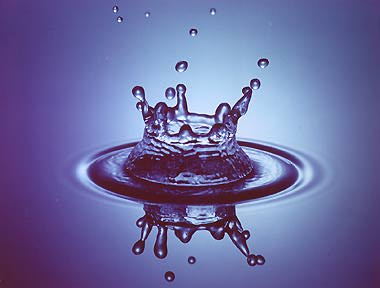
\includegraphics[height=42mm]{./Figures/splash.jpg}}
 \put(15, -17){\includegraphics[height=42mm]{../FIGURES/Wasa.jpg}}
  \end{picture}

  \vspace{2mm}
  
  \begin{flushright}
    
    \Large
   	\bf
    
    2. Forces de pression dans un fluide -- Hydrostatique

  \end{flushright}


\end{frame}



\handout{
\begin{frame}{Sommaire}
\small  
\hspace*{2mm}
\begin{tabular}{cc}
		%&
  		\begin{minipage}{62mm}
  			\tableofcontents[]
      \vspace{15mm}
  		\end{minipage}
  		&   
  		\begin{minipage}{60cm}
		  \vspace*{-5mm}  
  			%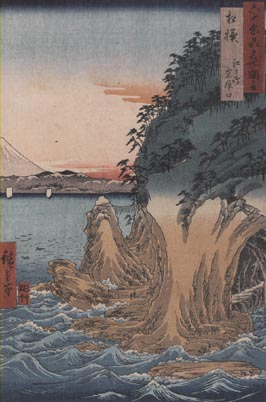
\includegraphics[width=40mm]{vagues.jpg} 
  		\end{minipage}
  	\end{tabular}
\vspace{0mm}
\end{frame}
}

%\setcounter{section}{1}
\nohandout{\section{Forces de pression dans un fluide -- Hydrostatique}}

\subsection{ Pression (et température) : signification physique. 
} 


%\subsubsection{Description d'un fluide (II) : point de vue microscopique}


%--------------------------------------------------------------------------------------------------


%%%%%%%%%%%%%%%%%%%%%
\begin{frame}{Pression : définition(s)}

\small

Définitions : 

\begin{itemize}[<+-| alert@+>]
\item Définition Thermodynamique : (pour un système simple)

Pression = variable intensive reliée aux échanges d'énergie mécaniques 
(liée au mouvement d'une frontière, et donc à la modification du volume) 

$$
p = - {\left( \frac{\partial E}{\partial V} \right)}_{S} = \rho {\left( \frac{\partial e}{\partial \rho} \right)}_{s} 
$$  


(Définition théorique mais inutilisable avec les modèles de fluides les plus courants, pour lesquels $e = e(T,P)...$)

Corollaire : à l'équilibre thermodynamique $p$ est uniforme ; cf. cours thermo.


\item Définition mécanique 

Pression = force surfacique normale exercée par un fluide au repos sur une surface matérielle (frontière avec une paroi solide)
 ou fictive (séparant avec un autre domaine fluide).

En considérant une {\em surface élémentaire} (au sens de la MMC) $dS$ de normale $\vec{n}_{{\cal F} \rightarrow {\cal S} }$, la force élémentaire exercée par le fluide sur la surface vaut 

$$
d \vec{f}_{{\cal F} \rightarrow {\cal S} } = p  \vec{n}_{{\cal F} \rightarrow {\cal S} } d S
$$

\pause

\color{gris}{
\tiny
 Lien entre les 2 définitions :

En supposant que la surface $\cal S$ subit un déplacement {\em élémentaire}  (au sens de la thermo) $\delta \vec X$, le travail reçu par le fluide vaut:

$$
\delta W = \iint_{\cal S} \delta \vec{X} \cdot (p  \vec{n}_{{\cal S} \rightarrow {\cal F} } d S )
$$

En supposant la pression uniforme il vient $\delta W = - p dV$ avec $dV = 
\iint_{\cal S} \delta \vec{X} \cdot \vec{n}_{{\cal F} \rightarrow {\cal S} } d S$.

} 

\pause 
\item Définition cinétique :

La pression est un {\em flux surfacique de quantité de mouvement microscopique normale} transféré par les particules à une paroi ou à un domaine fluide adjacent.



\end{itemize}


\end{frame}


\begin{frame}{Notions de théorie cinétique}
%--------------------------------------------------------------------------------------------------

\small

%Point de vue microscopique (échelle microscopique $\ell$) : 

%Description individuelle du mouvement des particules (masse $m_i$, vitesse $\vec{v}_i(t)$).



Sous l'hypothèse du milieu continu $Kn \ll 1$ (cf. chap. 1), 
on peut faire des moyennes sur le VER et définir successivement :

\smallskip 
\pause
- La masse volumique

$$
\rho = \frac{ N m_p}{V}   ,
$$

\pause 
- La vitesse moyenne 
$$
\vec{u} = \frac{1}{N} \sum_{i \in V} \vec{v}_i  ,
$$



\pause
- La vitesse quadratique moyenne 


$$
v_q^2 =  \frac{1}{N} \sum_{i \in V} \frac{| \vec{v_i} - \vec{u}|^2}{2}
$$

\pause 
Cette dernière quantité permet de définir la Température cinétique :

$$
T = \frac{ m_p v_q^2}{3 k_b}  \qquad ( k_B = 1.38 \cdot  10^{-23} m^2 kg s^{-2} K^{-1} \mbox{constante de Boltzmann} )
$$  
 

Remarque : 
on peut aussi écrire cette relation sous une forme plus pratique à l'échelle macroscopique :

$$
T = \frac{ M v_q^2}{3 R}  =  \frac{v_q^2}{3 r}
$$


%\pause

%\medskip

%On peut par ailleurs définir une échelle microscopique $\ell$ %caractérisant les interactions entre particules.


\end{frame}




%%%%%%%%%%%%%%%%%%%%%%%%%%%%%%%
\begin{frame} {Origine physique de la pression : cas des gaz}

\small 

Dans un gaz {\em parfait} les particules n'interagissent que par des collisions (sur une paroi ou entre elles).


%a pression est une variation de {\em quantité de mouvement normale} 
%liée aux collisions (sur une surface solide) ou aux particules traversant la surface (pour une surface entre deux domaines fluides adjacents).
\medskip

{\color{vert} Illustrations avec le programme kinetics.m}

\pause
\medskip 

%Pression = (densité) x (agitation thermique).

%c.a.d. $p = \rho r T$ (loi des gaz parfaits)

La théorie cinétique permet de calculer $p$ en fonction des propriétés microscopiques (cf. Guyon, Hulin, Petit ; cours Thermo L2).

\medskip

Calcul simplifié de la force de pression exercé sur une paroi 
(identifée à la variation de qdm due aux impacts sur celle-ci) :


$$
p =   \underbrace{\frac{n}{6} v_q}_{\mbox{ flux de particules impactant la paroi}}  \times  \underbrace{ 2 m_p v_q}_{\mbox{ variation de qdm au cours d'un impact}}
$$

où $n=N/V = \rho/m_p$ est la densité volumique de particules.

Ce qui aboutit à l'équation d'état mécanique :

$$
p = \rho r T
$$

\smallskip





\pause
\bigskip

{\bf Remarque :} 

Dans un gaz, l'échelle microscopique $\ell$ caractérisant les interactions interparticules est le  "libre parcours moyen" 

$$\ell  = \frac{1}{n \pi a^2}  $$ 

où $n = \frac{N}{V} = \frac{\rho}{m_p}$ est la densité volumique de particules et $a$ le rayon "effectif" des particules (rayon efficace de choc).

Ordres de grandeur : $a \approx 0.1 nm = 10^{-10} m$; 
 $\ell \approx 100 nm $ (dans l'air à température et pression ambiantes).
 






\end{frame}

%%%%%%%%%%%%%%%%%%%%%%%%%%%%%%%%%%%%
\begin{frame} {Origine physique de la pression : cas des liquides}

\small 
Dans un liquide la pression est due aux liaisons (répulsives ou attractives) entre les molécules adjacentes.

\smallskip

La pression dans un liquide peut ainsi être négative (liaisons majoritairement attractives).

Cet état est métastable du point de vue thermo mais qui peut tout de même être observé dans la nature (sève dans les arbres de plus de 10m...)

\medskip

NB : les liaisons sont très "raides" et il est difficile de faire varier la distance inter-molécule.

Ceci justifie que les liquides sont très peu compressibles. 

\smallskip

Modèle "liquide incompressible, indilatable" : $\rho = \rho_0 = C_{te}$ . 

$\partial \rho / \partial p \approx 0 $ $\rightarrow$ $\rho$ et $p$ sont découplés.  

Dans ce modèle $p$ devient une variable mécanique qui n'est plus reliée à la thermodynamique.



\pause
\bigskip

{\bf Remarque :} 

Dans un liquide, l'échelle microscopique $\ell$ caractérisant les interactions interparticules est la distance inter-moléculaire

$$\ell  = n^{-1/3}  $$ 

où $n = \frac{N}{V} = \frac{\rho}{m_p}$ est la densité volumique de particules.

Ordre de grandeur :  $\ell \approx 1 nm $ 
 






\end{frame}

\subsection{Hydrostatique}

\subsubsection{Loi de l'hydrostatique}

%%%%%%%%%%%%%%%%%%%%%%%%%%%%%%
%--------------------------------------------------------------------------------------------------
\begin{frame}{Application : statique des fluides}
%--------------------------------------------------------------------------------------------------

\small
\textbf{Loi de l'hydrostatique} \medskip

Pour un fluide au repos dans un référentiel galiléen, soumis à un champ de force massique $\myvec{g}$ constant (en général la gravité) :

$$
	\gradient p = \rho \myvec{g}
$$

\pause 
Démonstration :

%$(i)$ 
Equilibre des forces sur un volume élémentaire de fluide $dV$, de masse $dm = \rho\, dV$ :
$$
\sum d\myvec{F}_{ext \rightarrow dV} = \myvec{0}
$$

%$(ii)$ Equilibre d'un volume $\cal V$ 

\bigskip
\pause

Application \textcolor{vert}{\sl (exercices)} : 

\smallskip

1/ Liquide incompressible de masse volumique uniforme $\rho$ (océan) 

$$
 p = p_0 - \rho g z
$$

(Modèle plus précis incluant la thermocline, cf exercice 2.3)



\bigskip

2/ Gaz parfait (atmosphère d'une planète ou d'une étoile)

Modèle d'atmosphère isotherme :
$$ 
p = p_0 e^{-\frac{ g z}{rT_0}}
$$



%Cas adiabatique (exercice) :
%$$
%p = 

(Modèle d'atmosphère standard, cf. exercice 2.2).

\end{frame}




%--------------------------------------------------------------------------------------------------
\begin{frame}{Statique des fluides en repère non galliléen}
%--------------------------------------------------------------------------------------------------

\small
\textbf{Cas d'un référentiel non galliléen} \medskip

Pour un fluide "au repos" dans un référentiel non galliléen il faut ajouter les pseudo-forces d'inertie 

(accélération d'entrainement $\myvec{a}_e$). 

$$
	\gradient p = \rho \left( \myvec{g}+ \myvec{a}_e \right)
$$



\medskip

Exemple d'un liquide dans un récipient cylindrique en rotation ("Seau de Newton") :
$$
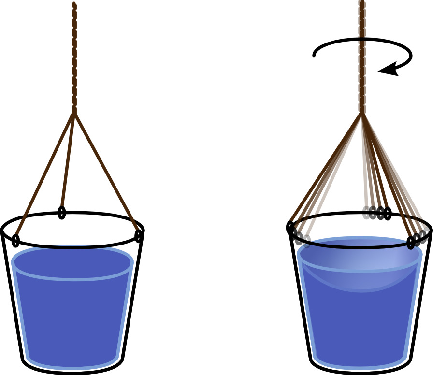
\includegraphics[width=.5\linewidth]{Figures/NewtonsBucket.png}
$$


\textcolor{vert}{\sl (Exercice classique)}  

Les surfaces de même pression (surfaces isobares) sont des paraboles 

\color{gris}{(y compris la surface libre en négligeant la tension superficielle). }



%\textbf{Théorème et poussée d'Archimède} \medskip

%On montre \textcolor{vert}{\sl (exercice)} que la résultante des efforts de pression sur la surface
%d'un corps immergé dans le champ de pesanteur est une force qui est l'opposé du poids du volume de fluide occupé par le corps, et qui s'applique au centre de gravité de ce volume de fluide, appelé centre de poussée.

%\vspace{20mm}

\end{frame}

\subsubsection{Efforts de pression sur une surface}

\begin{frame}{Efforts de pression sur une surface}

\small

Soit une surface ${\cal S}$ (matérielle ou non) délimitant 
(partiellement ou totalement) un fluide $F$ à l'équilibre.
Soit $M$  un point courant de ${\cal S}$  et 
$\vec n_{{\cal F}\rightarrow {\cal S}}$  un vecteur 
normal orienté du fluide vers la surface ("entrant").
Les efforts  exercés par $F$ sur ${\cal S}$ 
(efforts hydrostatiques) sont données par le torseur suivant :

\medskip

$$ 
\left\{ {\cal F} \rightarrow {\cal S} \right\} =  \torseur{A}{\vec R}{\vec M_{A}} =
= \torseur{A}
{\displaystyle \iint_{\cal S} p(M) \vec n_{{\cal F}\rightarrow {\cal S}} d S}
{ \displaystyle \iint_{\cal S}  \overrightarrow{ AM }\times p(M) \vec n_{{\cal F}\rightarrow {\cal S}} d S}
$$

\medskip

{\bf Remarques : }
\pause

- Dans le cas d'une surface fermée délimitant un objet $\Omega$ plongé dans le fluide, la convention habituelle est de noter 
$\vec n$ la normale sortante (par rapport à l'objet). Dans ce cas on peut utiliser les formules 
précédentes en écrivant $\vec n_{{\cal F}\rightarrow \Omega} = -\vec n$.

\pause 
- On appelle  {\em point d'application} "le" point $C$ tel que $\vec M_{C}=0$ 

(définition non rigoureuse car ce point n'est pas unique ; on peut choisir n"importe quel point situé sur la "droite d'action" du torseur).


\medskip

\textcolor{vert}{\sl Exercices classiques :} 

- Calculez la résultante des forces de pression sur un barrage rectangulaire vertical de hauteur $H$. 
Montrez que le point d'application est situé à une altitude $H/3$ par rapport au fond.

- Barrage triangulaire (exercice a préparer avant le TD, corrigé sur moodle).

\end{frame}


\subsubsection{Poussée d'Archimède}

%%%%%%%%%%%%%%%%%%%%%
\begin{frame}{Théorème d'Archimède}
\small

\pause

{\em 
"Tout corps plongé entièrement dans un ou plusieurs fluides au repos,
subit de la part du (des) fluide(s) une force verticale, dirigée 
vers le haut, égale en intensité au poids du volume de fluide 
déplacé, et qui s'applique au centre de gravité $G_f$ 
du(des) fluide(s) déplacé(s)."
}

\pause
\medskip

En termes plus précis, la poussée d'Archimède correspond au torseur suivant :

$$
\left\{ {\cal A} \right\} = \torseur{G_f}{ \vec{\cal P}_{\cal A} = -M_f \vec{g}}{ \vec{\cal M}_{{\cal A},G_f} =   \vec 0}.
$$

Démonstrations : $(i)$ physique ; $(ii)$ mathématique.

\pause
\medskip

\paragraph{\bf Remarques :}

\begin{itemize}

\item en général $G_f \neq G$ ($G$ est le centre de gravité du corps 
considéré, et dépend de la répartition de masse à l'intérieur de celui-ci). 

\item Si le fluide déplacé a une masse volumique constante $\rho_f$, alors
$M_f = \rho_f V$, et le point $G_f$ correspond au centre géométrique
$C$ de l'objet.

\item La somme de la force de gravité $M\vec g$ et de la poussée d'Archimède 
est parfois appelée "poids relatif" ou "force de flottabilité" (buoyancy) :
$\vec F = ( M - M_f ) \vec g$. 

\end{itemize}

\end{frame}



\subsubsection{Equilibre des corps flottants}


%%%%%%%%%%%%%%%%%%%%%
\begin{frame}{Equilibre des corps flottants (1)}

\small
\paragraph{\bf Cas d'un corps de masse $m$ et volume $V$ entièrement immergé dans un fluide homogène de masse volumique 
$\rho_f$ (sous-marin ou montgolfière) } 

\medskip

Recherchons les conditions d'équilibre sous l'effet de son poids $\left\{ {\cal G} \right\}$ et de la poussée d'Archimède $\left\{ {\cal A} \right\} $.

\medskip \pause 

{\bf Equilibre des résultantes :} $ m = \rho_f V$.

$ \qquad \rightarrow$ Conséquence : le véhicule doit pouvoir contrôler sa masse en fonction du milieu environnant !

\smallskip \pause

{\bf Equilibre des moments :} $ \overrightarrow{CG} \wedge m \vec g = \vec{0}$.

$ \qquad \rightarrow$ Conséquence : $C$ et $G$ doivent être alignés verticalement 

$\qquad \quad$ (position stable si $G$ est en dessous de $C$).



\end{frame}



%%%%%%%%%%%%%%%%%%%%%
\begin{frame}{Equilibre des corps flottants (2)}

\small

\paragraph{\bf Cas d'un corps de masse $m$ partiellement immergé dans un liquide homogène de masse volumique 
$\rho_f$ (bateau) } 


%Recherchons les conditions d'équilibre sous l'effet de son poids $\left\{ {\cal G} \right\}$ et de la poussée d'Archimède $\left\{ {\cal A} \right\} $.

\bigskip \pause 

{\bf Equilibre des résultantes :} $ m = \rho_f V_0$ où $V_0$ est le "volume de carène" (volume de la partie immergée)

$ \qquad \rightarrow$ Conséquence : l'équilibre reste possible si $m$ varie. 

\bigskip \pause

{\bf Equilibre des moments :} 

$$
\sum \vec{M} =  \overrightarrow{OG} \wedge m \vec{g} + \overrightarrow{OC_\phi} \wedge \vec{\cal P}_{\vec A} =  \ \overrightarrow{C_\phi G} \wedge m \vec{g} 
$$

\smallskip 
\pause

Subtilité : lorsque l'inclinaison (gîte) $\phi$ varie, le centre de carène $C_\phi$ se déplace ! 

\smallskip 
\pause

On peut montrer qu'il existe un point {\em fixe} $M$ appelé {\em Métacentre de roulis} tel que 
$\vec{\cal M}_{{\cal A},M} = \vec 0 \quad \forall  \phi$ (dans la limite $\phi \ll 1$).

\smallskip 
(cad. la droite d'action de la poussée d'Archimède passe par $M$  $\forall  \phi$) 

\smallskip
Soit :

$$\sum \vec{\cal M} =   \overrightarrow{MG} \wedge m \vec{g} \quad \forall \phi \quad \mbox{ ( dans la limite } \phi \ll 1 ) $$

\smallskip 
\pause

La position de $M$ est donné par la formule de Bouguier : 

$C_0 M = \frac{ L b^3 }{12 V_0}$ 

( pour une carène prismatique, de longueur $L$ et largeur à la flottaison $b$ ; $C_0$ étant le centre de carène de la position de référence $\phi = 0$).

\medskip \pause

$ \qquad \rightarrow$ Conséquence : la position $\phi = 0$ est stable si {\bf $G$ est en dessous de $M$.}



\end{frame}




\subsection{Tension superficielle}

%--------------------------------------------------------------------------------------------------
\begin{frame}{Tension superficielle : mise en évidence expérimentale}
%--------------------------------------------------------------------------------------------------

Expériences avec un film de savon :


%\href{https://www.math.hmc.edu/~jacobsen/demolab/soapfilm.html}{\beamergotobutton{https://www.math.hmc.edu/~jacobsen/demolab/soapfilm.html}}
%\verb|

\medskip

\href{https://www.math.hmc.edu/~jacobsen/demolab/soapfilm.html}{
 \textcolor{blue}{
https://www.math.hmc.edu/~jacobsen/demolab/soapfilm.html
}
}

\bigskip


Origami capillaire :

\medskip

%\begin{verbatim}
%\textcolor{blue}{
%https://www.youtube.com/watch?v=n51Vi3rv\_kA
%\end{verbatim}
\href{https://www.youtube.com/watch?v=n51Vi3rv_kA}{\textcolor{blue}{https://www.youtube.com/watch?v=n51Vi3rv\_kA}}
 

https://www.google.com/imgres?imgurl=http%3A%2F%2Fwww.brandeis.edu%2Fnow%2F2012%2Fjanuary%2Fimages%2Fskimmer405.jpg&imgrefurl=http%3A%2F%2Fwww.brandeis.edu%2Fnow%2F2012%2Fjanuary%2Fsurface.html&docid=rbTdmv6-P5iwCM&tbnid=m7xfpdX5vRGt8M%3A&vet=1&w=405&h=270&client=safari&bih=712&biw=1213&q=surface%20tension&ved=0ahUKEwisqaPxzrfRAhUJMhoKHRzbABo4ZBAzCAIoADAA&iact=mrc&uact=8



\end{frame}

%%%
%Quelques bons sites :

%https://fr.wikipedia.org/wiki/Tension\_superficielle
%Quelques explications fausses :

%http://www.sita-process.com/information-service/process-parameter-surface-tension/overview/


\begin{frame}{Tension superficielle : modélisation physique}

\small

\textbf{Forces linéiques : la tension de surface} \medskip

Si le volume de fluide $\Omega$ est traversé par une interface entre deux fluides non miscibles (fluide 1 et fluide 2),
le fluide contenu dans $\Omega$ est soumis à une force de tension le long de la ligne $\cal L$
intersection de la frontière de $\Omega$ avec l'interface :

\medskip

\centerline{$ \color{rouge} \displaystyle d\myvec{F}_{{\cal L} \rightarrow \Omega}  = \gamma \, dl \; \myvec{n}_{\cal L} $}
\begin{itemize}
\item[]
	o{\`u} $dl$ : longueur élémentaire le long de $\cal L$
\item[]
	et $\myvec{n}_{\cal L}$ : vecteur unitaire tangent à l'interface, $\perp$ à $\cal L$, et sortant par rapport au domaine $\Omega$
\end{itemize}

\smallskip

\pause

Le coefficient de \textcolor{rouge}{tension de surface} $\gamma$ 
correspond à une force par unité de longueur (N/m) 
\\
ou de manière équivalente à une énergie par unité de surface (J/m$^2$).



\medskip

Sa valeur est une propriété physique de l'ensemble (fluide 1/ fluide 2)
(ex. $\gamma = 0.07$ N/m pour une interface eau/air)

\pause

\medskip

{\bf  \textsl{Loi de Laplace} (rappels L2)}


\begin{itemize}
\item[]
On montre que la tension de surface conduit à un saut de pression 
de part et d'autre de l'interface :

\centerline{$ \displaystyle \color{rouge} p_1 - p_2 = \frac{2 \gamma}{\cal R} 
                                      = \gamma \, \left (\frac{1}{\cal R'}+\frac{1}{\cal R''}\right)$}
\item[]
o{\`u} $\cal R$ : rayon de courbure local de l'interface (centre de courbure dans le fluide 1)
\item[]
\myhskip{o{\`u}} $\cal R'$ et $\cal R''$ : rayons de courbure principaux en 3D (cf. cours de géométrie différentielle)
\end{itemize}


\pause

\smallskip

{\bf  \textsl{Angle de contact} (rappels L2)}

Au niveau de la ligne triple (fluide 1 / fluide 2 / paroi solide), on constate que l'angle de contact $\theta$ est fixé : $\theta = \theta_E$

$\theta_E$ est une propriété physique de l'ensemble  (fluide 1 / fluide 2 / paroi solide). 

Si $\theta_E < \pi/2$ on parle de surface hydrophile (exemple : eau/air/verre).

Si $\theta_E > \pi/2$ on parle de surface hydrophobe (exemple : eau/air/téflon).

\end{frame}

%--------------------------------------------------------------------------------------------------
\begin{frame}{Compétition entre capillarité et pesanteur}
%--------------------------------------------------------------------------------------------------

\small

\begin{overprint}

\onslide<1>   
  
\begin{center}
	\begin{picture}(60, 70)
   	\put(0, 0){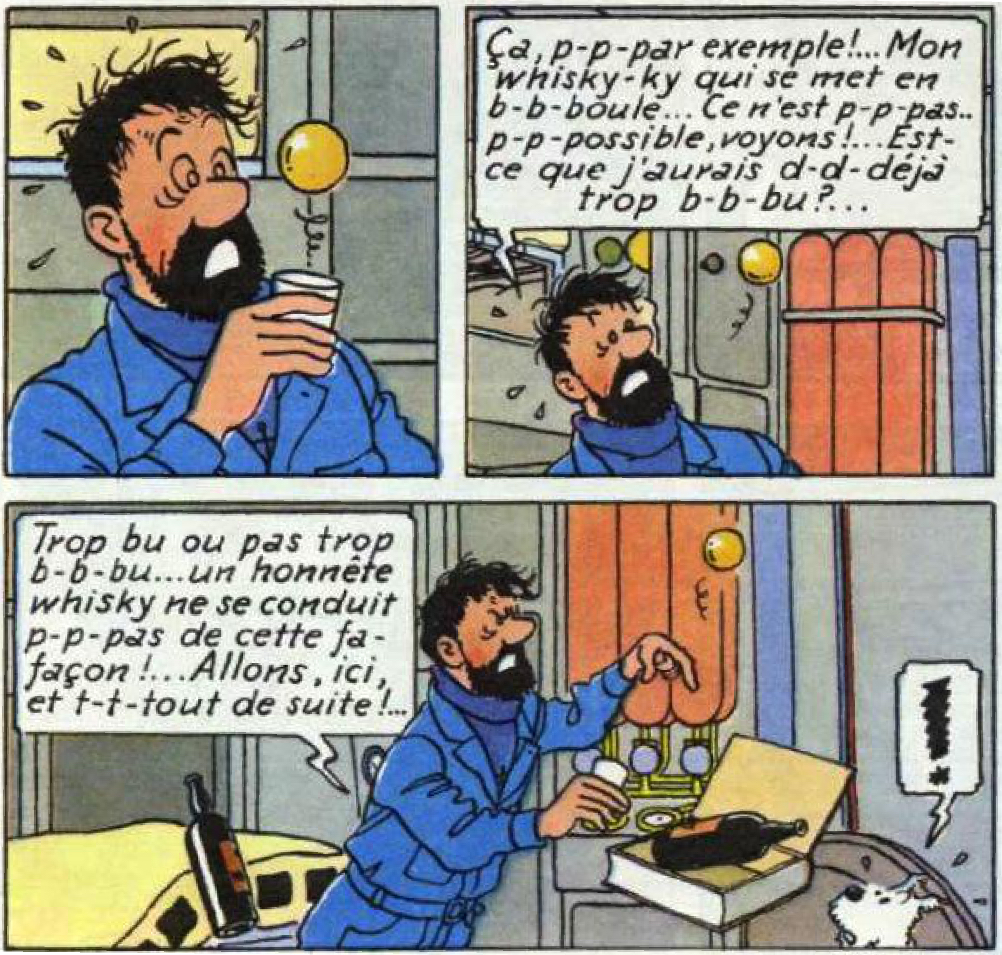
\includegraphics[height=60mm]{whisky_Haddock.jpg}}
	\end{picture}
\end{center}

\onslide<2>   

\vspace{3mm}


Le nombre sans dimension permettant de comparer gravité et capillarité est 
le nombre  de \textcolor{rouge}{\bf Bond} :

$$ \color{rouge}
\Bond = \frac{\rho g L^2}{\gamma}
$$

\medskip
o{\`u} $L$ désigne l'échelle de longueur caractéristique
du phénomène étudié 
\\
 (par ex. le diamètre du verre de whisky du Capitaine Haddock\ldots)



\bigskip

 ce nombre peut s'écrire également 
$$ \color{rouge}
\Bond = \left ( \frac{L}{\ell_c}\right )^2 
$$
où $\color{rouge} \ell_c = \sqrt{\dfrac{\gamma}{\rho g}}  $  est l'échelle de longueur capillaire.


($ \ell_c = 2.7 mm$ Pour l'interface air/eau en gravité terrestre.) 






%\pause

\begin{picture}(0, 0)
	\put(90, 15){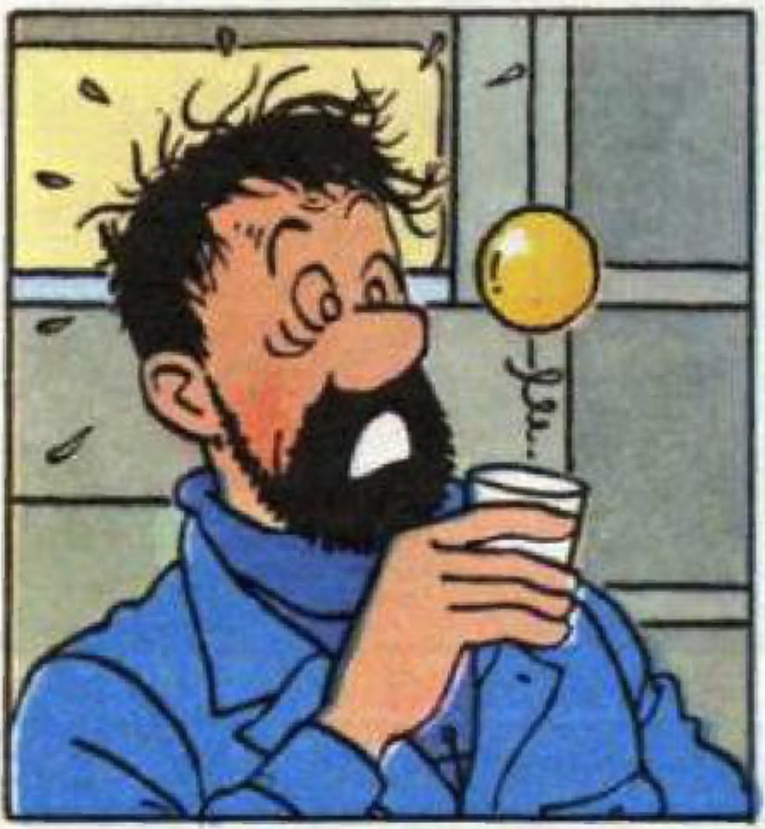
\includegraphics[width=20mm]{whisky_Haddock_crop.jpg}}
\end{picture}

\medskip

{\bf Interprétation :}

\medskip

\begin{itemize}
\item
	Si $\Bond \gg 1$ : pesanteur dominante (surface libre plane, horizontale).
\item
	Si $\Bond \ll 1$ : capillarité dominante (surface libre sphérique).
\item
	Si $\Bond = {\cal O}(1)$ : forces de gravité et capillarité comparables (surface libre solution d'un problème difficile...).	
	
\end{itemize}

\end{overprint}

\end{frame}


%\part{Viscosite}
%\section{Forces dans les fluides en mouvement (a remplir...)}
%\include{Chap3_Viscosite}
%\include{Chap4_Cinematique}

%

% !TEX root = NotesDeCours.tex

% ================================================================================================ 
% Page de titre :
% ================================================================================================


\part{Equations bilan}

%%%%%%%%%%%%%%%%%%%%%%%%%%%%%%%%%%%%%%%%%%%%%%%%%%%%%%%%%%%%%%%%%%%%%%%%%%%%%%%%%%%%%%%%%%
%\section{\bfseries Equations de bilan}
%%%%%%%%%%%%%%%%%%%%%%%%%%%%%%%%%%%%%%%%%%%%%%%%%%%%%%%%%%%%%%%%%%%%%%%%%%%%%%%%%%%%%%%%%%


\section{Equations Bilan}

\begin{frame}

  \color{bleu}

  \begin{flushleft}
    
    \Large
   	\bf
    
    Mécanique des fluides 

  \end{flushleft}
  
  \ligne{3} % remplace: \noindent \thickline{0.5mm}{150}

  \begin{flushright}

    \rm

    \textrm{David} \textsc{Fabre}
    
    \vspace{3mm}
    
    IMFT / UPS
    
    Département de Mécanique
    


  \end{flushright}

\begin{picture}(110, 25)(12, -20)
  \put( 15, -22){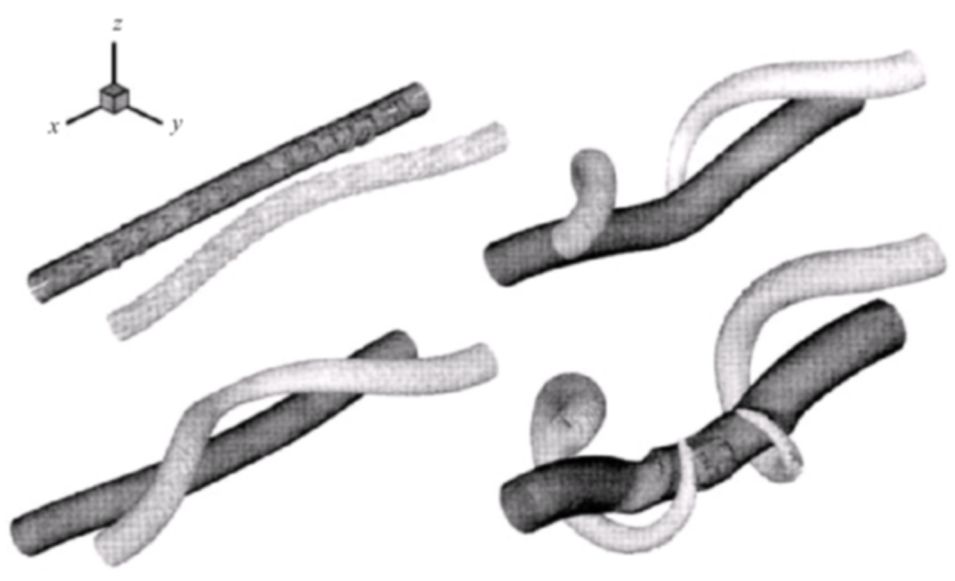
\includegraphics[width=65mm]{./Figures/MBG_fig19.png}}
  \put(84, -12){\color{gris} \slshape \small Interaction entre deux}    	
  \put(84, -15){\color{gris} \slshape \small tourbillons contrarotatifs}
  \put(84, -19){\color{gris} \slshape \small \rm \copyright\ \! IMFT}
  \put(16, 3){\color{gris} $(a)$}
  \put(16, -14){\color{gris} $(b)$}
  \put(74, 7){\color{gris} $(c)$}
  \put(74, -12){\color{gris} $(d\, )$}
\end{picture}
  \vspace{7mm}
  
  \begin{flushright}
    
    \Large
   	\bf
    
    5. Equations de bilan -- Régimes d'écoulements

  \end{flushright}

\end{frame}

%%%%%%%%%%%%%%%%%%%%%%%%%%%%%%%%%%%%%%%%%%%%%%%%%%%%%%%%%%%%%%%%%%%%%%%%%%%%%%%%%%%%%%%%%%
% Sommaire :
%%%%%%%%%%%%%%%%%%%%%%%%%%%%%%%%%%%%%%%%%%%%%%%%%%%%%%%%%%%%%%%%%%%%%%%%%%%%%%%%%%%%%%%%%%


\begin{frame}{Sommaire}

\small
  
\hspace*{2mm}
\begin{tabular}{cc}
		%&
  		\begin{minipage}{62mm}
  			\tableofcontents[firstsection=-2]
      \vspace{15mm}
  		\end{minipage}
  		&   
  		\begin{minipage}{60cm}
		  \vspace*{-5mm}  
  			%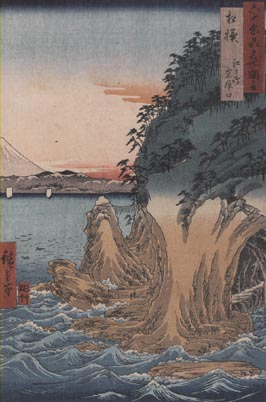
\includegraphics[width=40mm]{vagues.jpg} 
  		\end{minipage}
  	\end{tabular}

\vspace{0mm}

\end{frame}


%==========================================================================================
\subsection{Principes de conservation}
%=========================================================================================

%-----------------------------------------------------------------------------------------
\subsubsection{Ecriture générale d'un bilan}
%-----------------------------------------------------------------------------------------
\begin{frame}{Ecriture générale d'un bilan d'une quantité {\em extensive}}
%-----------------------------------------------------------------------------------------

\small

Considérons un système $\mathcal{S}$ donné (ex. la ville de Toulouse)

\smallskip

$\rightarrow$ comment décrire l'évolution au cours du temps d'une grandeur physique $F$ (extensive) \mytabbing{$\rightarrow$}
associée au système étudié (ex. le nombre de Toulousains, le nombre de voitures, la richesse totale des habitants, ...)
\bigskip

\begin{minipage}{100mm}

\begin{itemize}


\item<2->
	Equation-bilan entre deux {\em états d'équilibre} (forme privilégiée en thermo):
		\[
		\color{rouge} \Delta F = F_2 - F_1 = F_e+ F_p
	\]
\item<3->
	Bilan sous forme \textsl{variationnelle} :
	
	entre $t$ et $t+dt$, la variation de $F$ dans $\mathcal{S}$ s'écrit
	\[
		\color{rouge} dF = F(t+dt) - F(t) = \delta F_e+ \delta F_p
	\]
	où $\color{rouge} \delta F_e$ : échange ou \textcolor{vert}{interaction} ($<0$ ou $>0$) 
	avec l'\textbf{extérieur} entre $t$ et $t+dt$ \quad
	$\rightarrow$ flux ou transfert (ex. déménagements)
		
	\smallskip
	et $\color{rouge} \delta F_p$ : \textcolor{vert}{production} \textbf{interne} ($<0$ ou $>0$) pendant $dt$ \\
	(ex. naissances, décès, le temps qui passe\ldots) 

\smallskip
\item<4->

	Bilan sous forme \textsl{différentielle} :

	en divisant par $dt\rightarrow 0$, on en déduit l'équation d'évolution
  $$\color{rouge} \mydot{F} \equiv \ddt{F} = \mydot{F}_e + \mydot{F}_p$$
  	où $\mydot{F}_e$ : \textcolor{vert}{taux d'échange} avec l'extérieur 
	($\delta F_e = \mydot{F}_e\, dt$)
		
	et $\mydot{F}_p$ : \textcolor{vert}{taux de production} interne
	($\delta F_p = \mydot{F}_p\, dt$)
  
\end{itemize}

\end{minipage}

\begin{overprint}
\onslide<2->
\begin{picture}(0, 0)(-80, -10)
	\put(0, 0){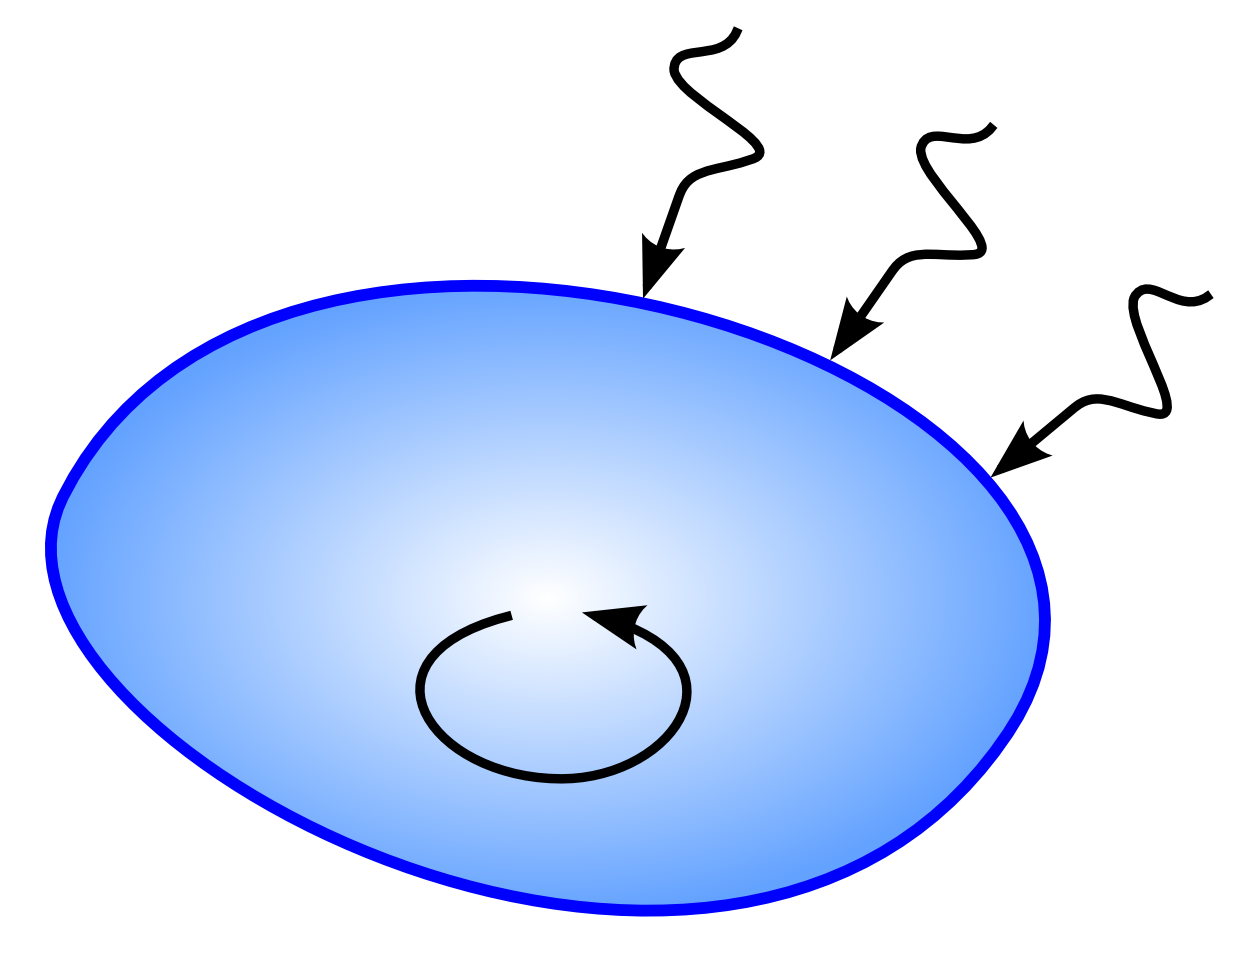
\includegraphics[width=25mm]{bilan.png}}
	\put(10, 8){$\delta F_p$}
	\put(8, 16){$\delta F_e$}
	\put(3, 8){$\mathcal{S}$}
\end{picture}
\end{overprint}

\vspace{5mm}

\end{frame}

%-----------------------------------------------------------------------------------------
\subsubsection{Les différents types de systèmes}
%-----------------------------------------------------------------------------------------
\begin{frame}{Les différents types de systèmes}
%-----------------------------------------------------------------------------------------

\small

\begin{itemize}%[<+-| alert@+>]
\item<1->
On appelle \textcolor{vert}{\bf système isolé} tout système qui n'échange pas avec l'extérieur
($\mydot{F}_e=0$) : \\
ni matière, ni quantité de mouvement, ni travail, ni chaleur.
\item<2->
Un domaine ou volume sera dit \textcolor{rouge}{\bf matériel} s'il est toujours 
constitué des mêmes particules \\ de matière au cours du temps.
C'est donc l'équivalent d'un système \textcolor{rouge}{\bf fermé},
qui n'échange pas de matière avec l'extérieur mais qui peut cependant échanger 
de la quantité de mouvement, du travail ou de la chaleur.
\item<11->
Un \textcolor{bleu}{\bf volume de contrôle} correspond 
à une portion donnée de l'espace, dont
la frontière peut être traversée par de la matière
entrante et sortante.
Il s'agit donc a priori
d'un système \textcolor{bleu}{\bf ouvert} qui peut échanger matière, quantité de mouvement, travail et chaleur avec l'extérieur.

\end{itemize}

\medskip

\begin{overprint}

\onslide<3>

\begin{center}
\begin{picture}(60, 35)(0, -5)
\put(0, 0){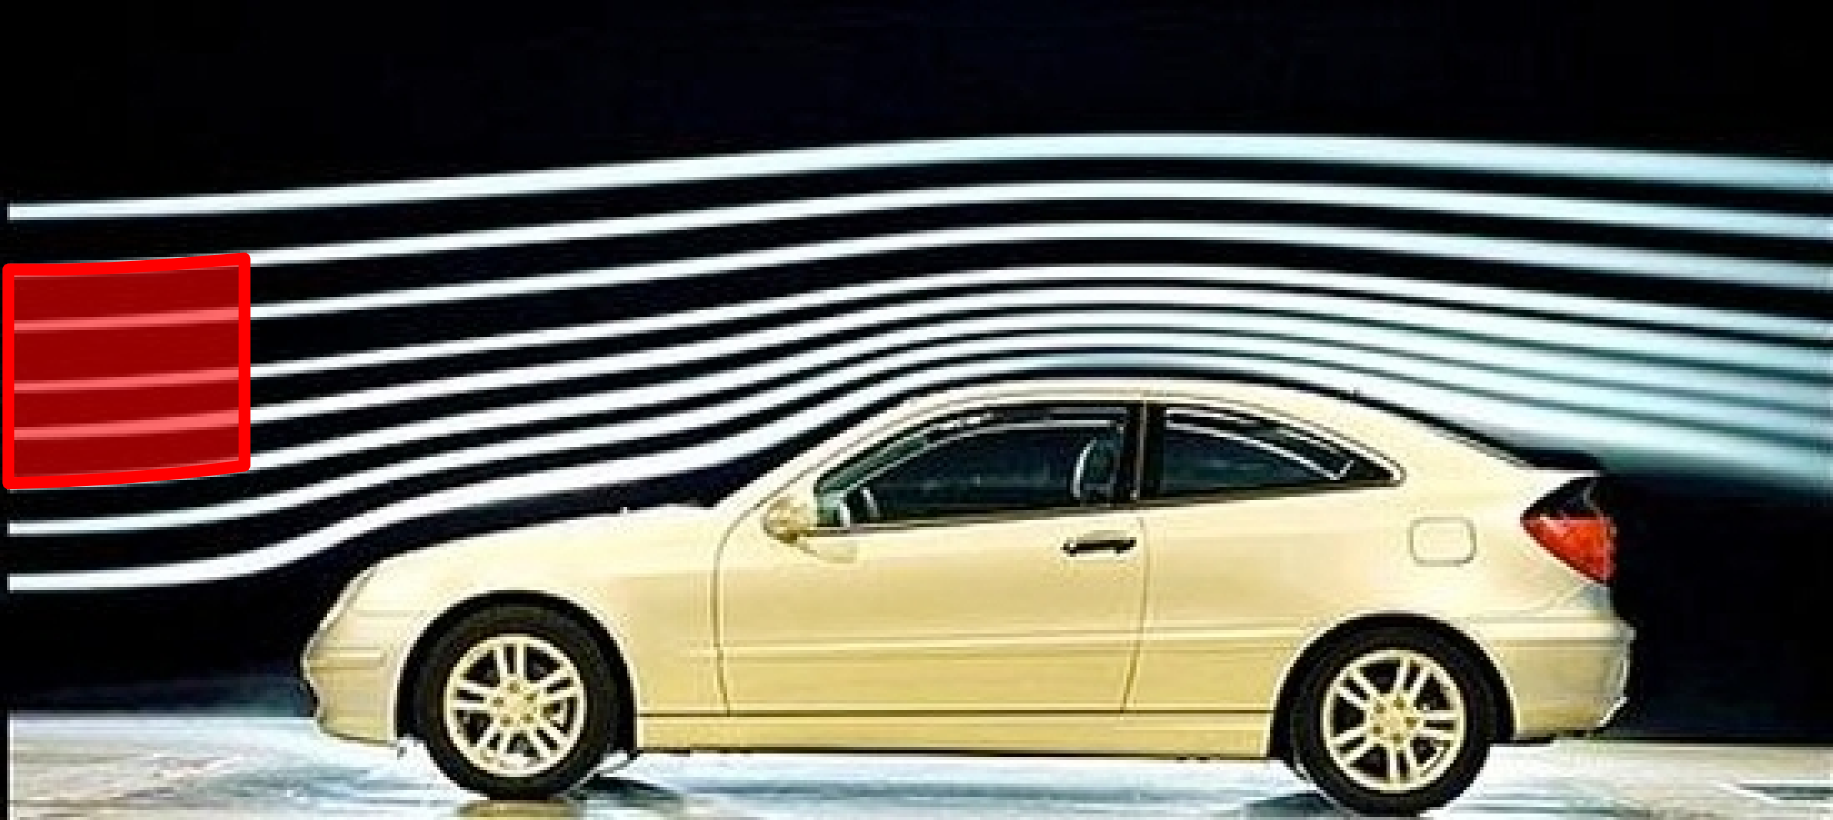
\includegraphics[width=60mm]{volume_materiel1.png}}
\put(22, -5){\color{rouge} Volume matériel $\mathcal{D}(t)$}
\end{picture}
\end{center}

\onslide<4>

\begin{center}
\begin{picture}(60, 35)(0, -5)
\put(0, 0){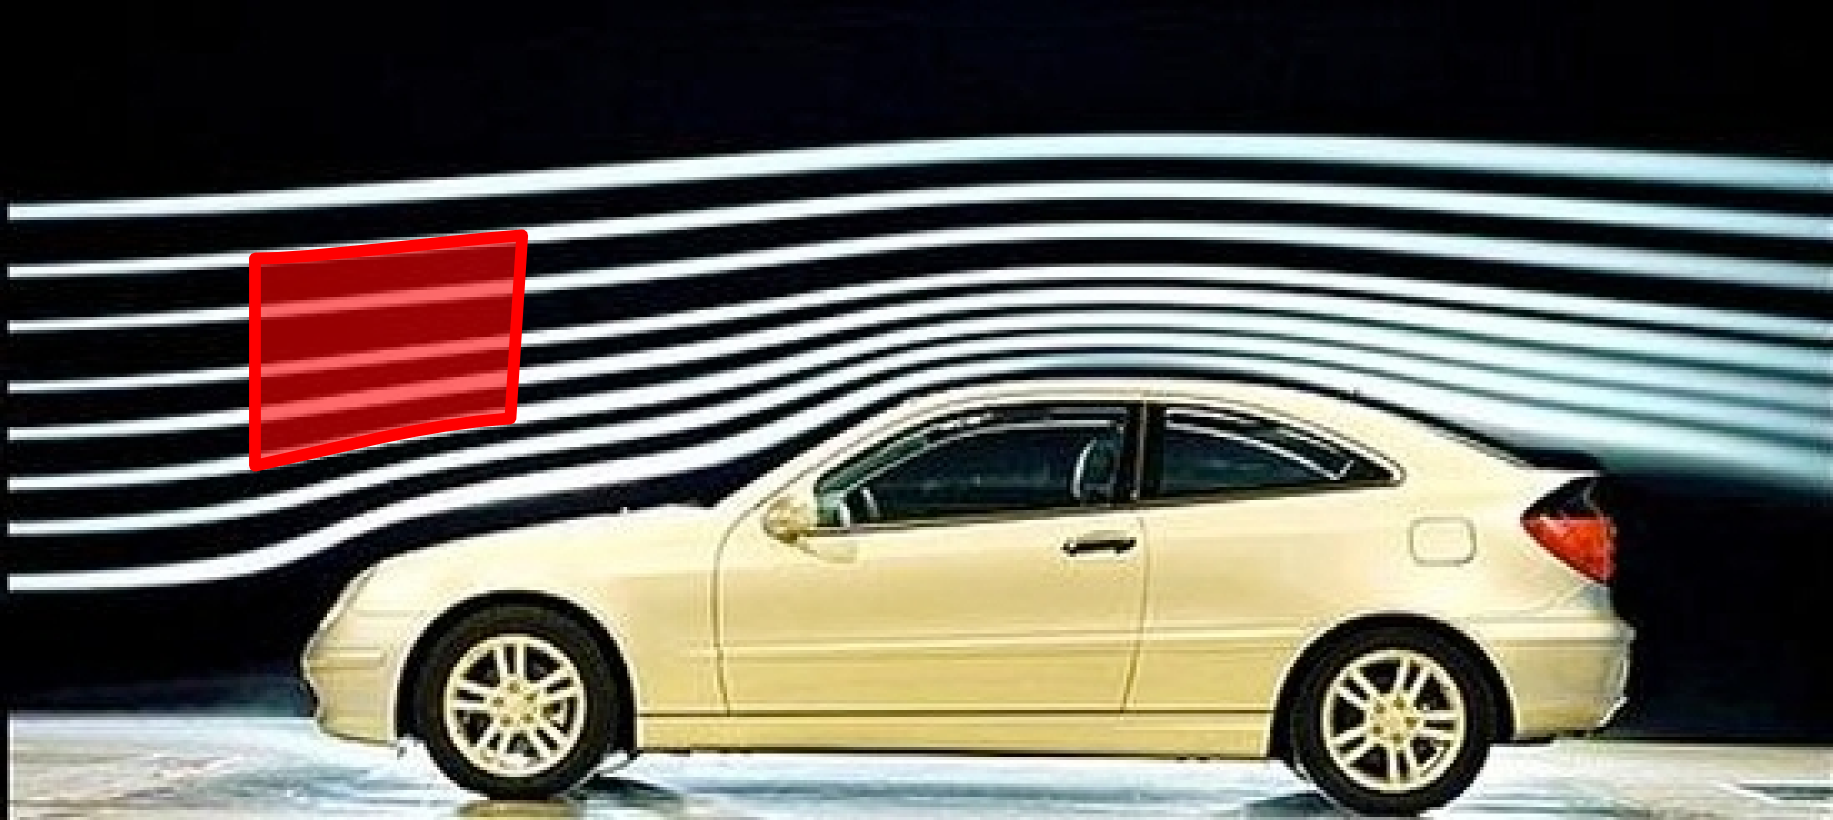
\includegraphics[width=60mm]{volume_materiel2.png}}
\put(22, -5){\color{rouge} Volume matériel $\mathcal{D}(t)$}
\end{picture}
\end{center}

\onslide<5>

\begin{center}
\begin{picture}(60, 35)(0, -5)
\put(0, 0){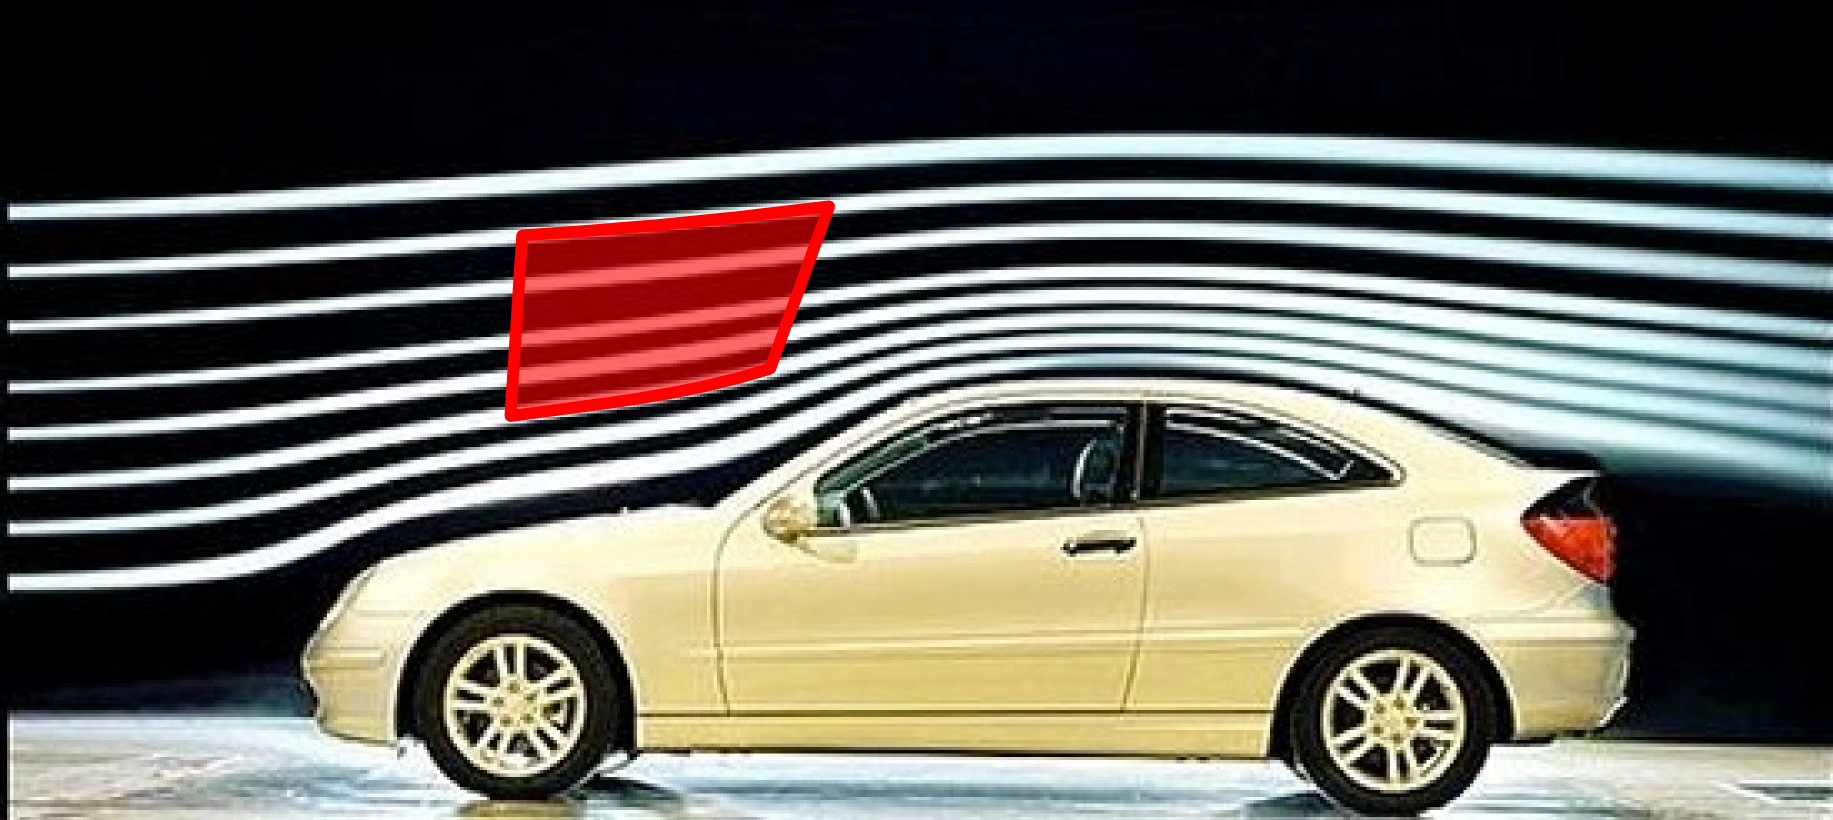
\includegraphics[width=60mm]{volume_materiel3.png}}
\put(22, -5){\color{rouge} Volume matériel $\mathcal{D}(t)$}
\end{picture}
\end{center}

\onslide<6>

\begin{center}
\begin{picture}(60, 35)(0, -5)
\put(0, 0){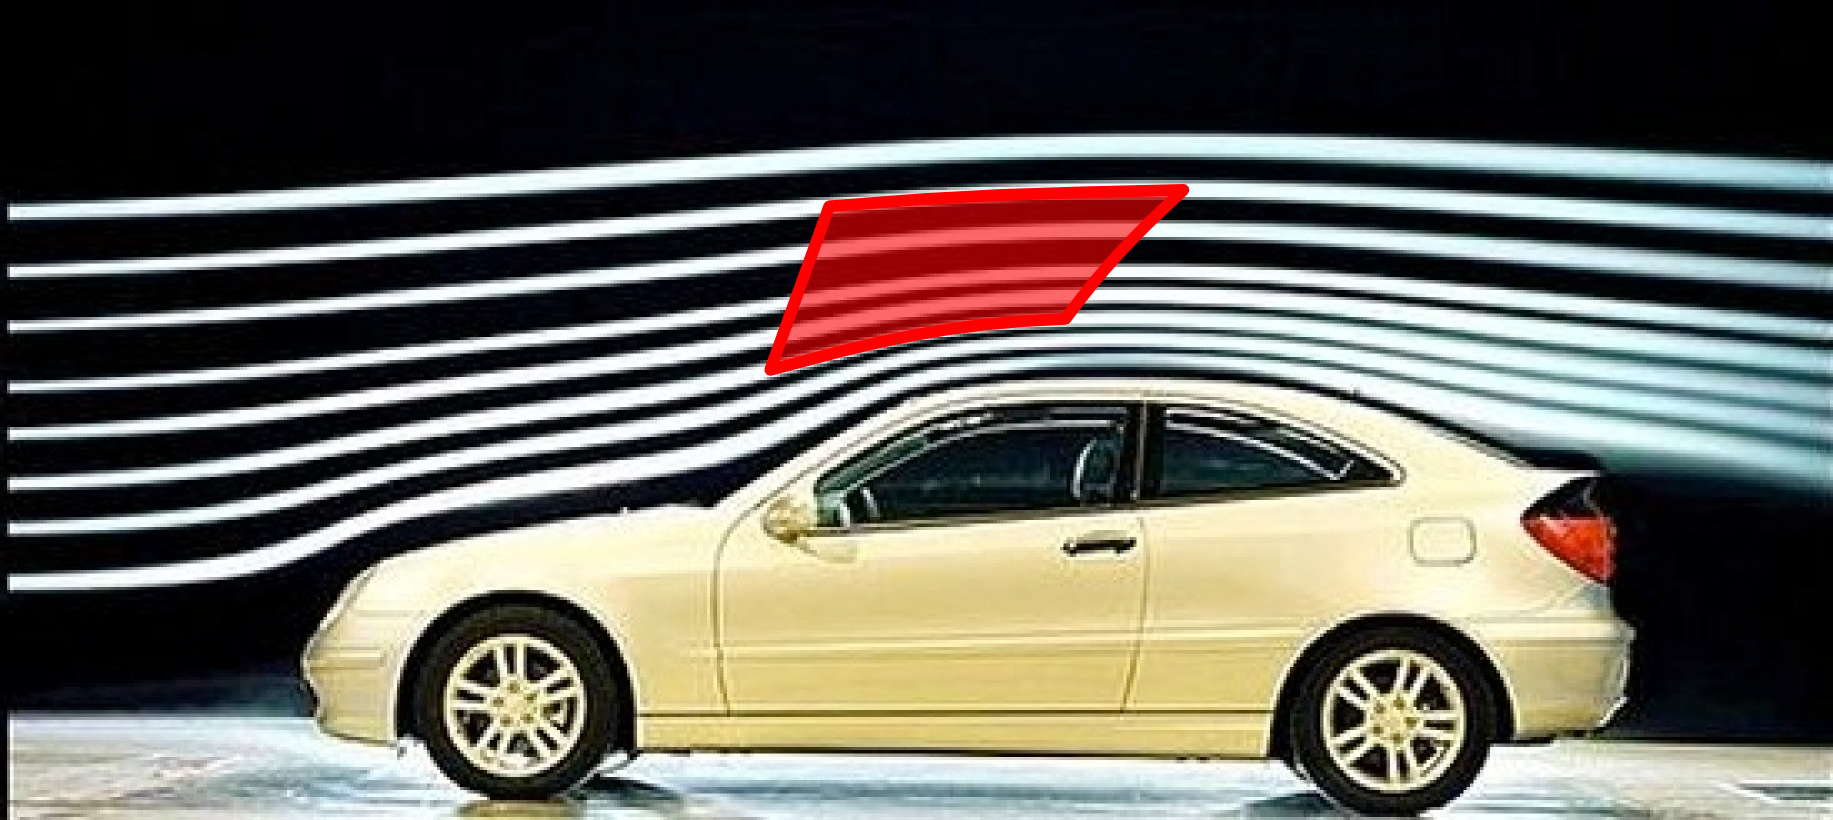
\includegraphics[width=60mm]{volume_materiel4.png}}
\put(22, -5){\color{rouge} Volume matériel $\mathcal{D}(t)$}
\end{picture}
\end{center}

\onslide<7>

\begin{center}
\begin{picture}(60, 35)(0, -5)
\put(0, 0){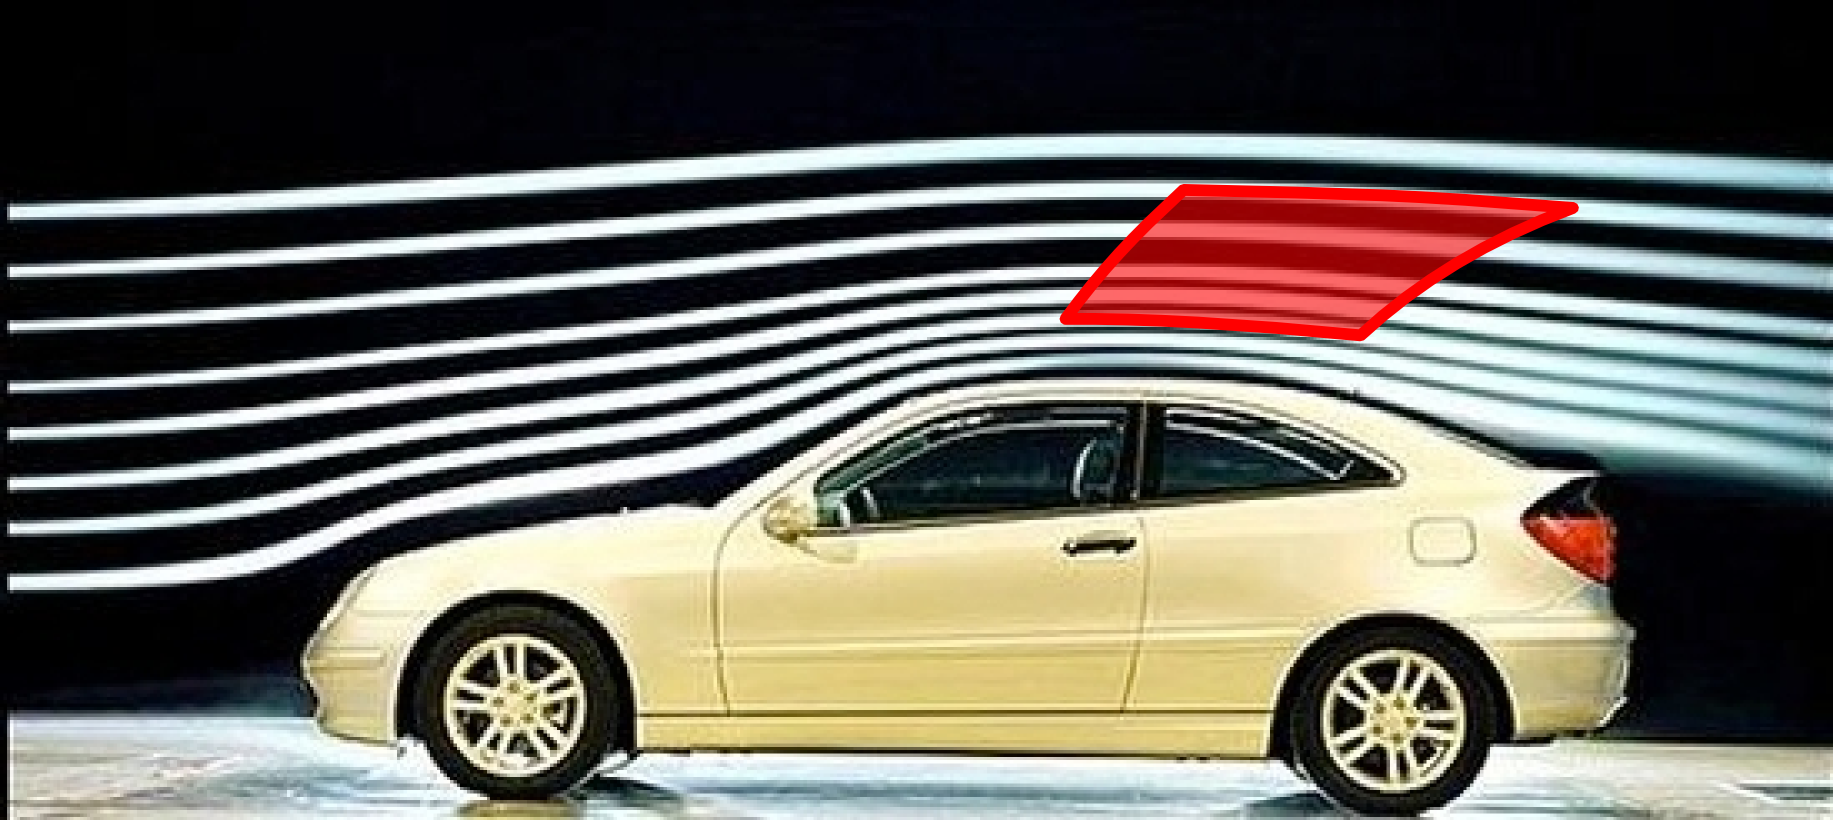
\includegraphics[width=60mm]{volume_materiel5.png}}
\put(22, -5){\color{rouge} Volume matériel $\mathcal{D}(t)$}
\end{picture}
\end{center}

\onslide<8>

\begin{center}
\begin{picture}(60, 35)(0, -5)
\put(0, 0){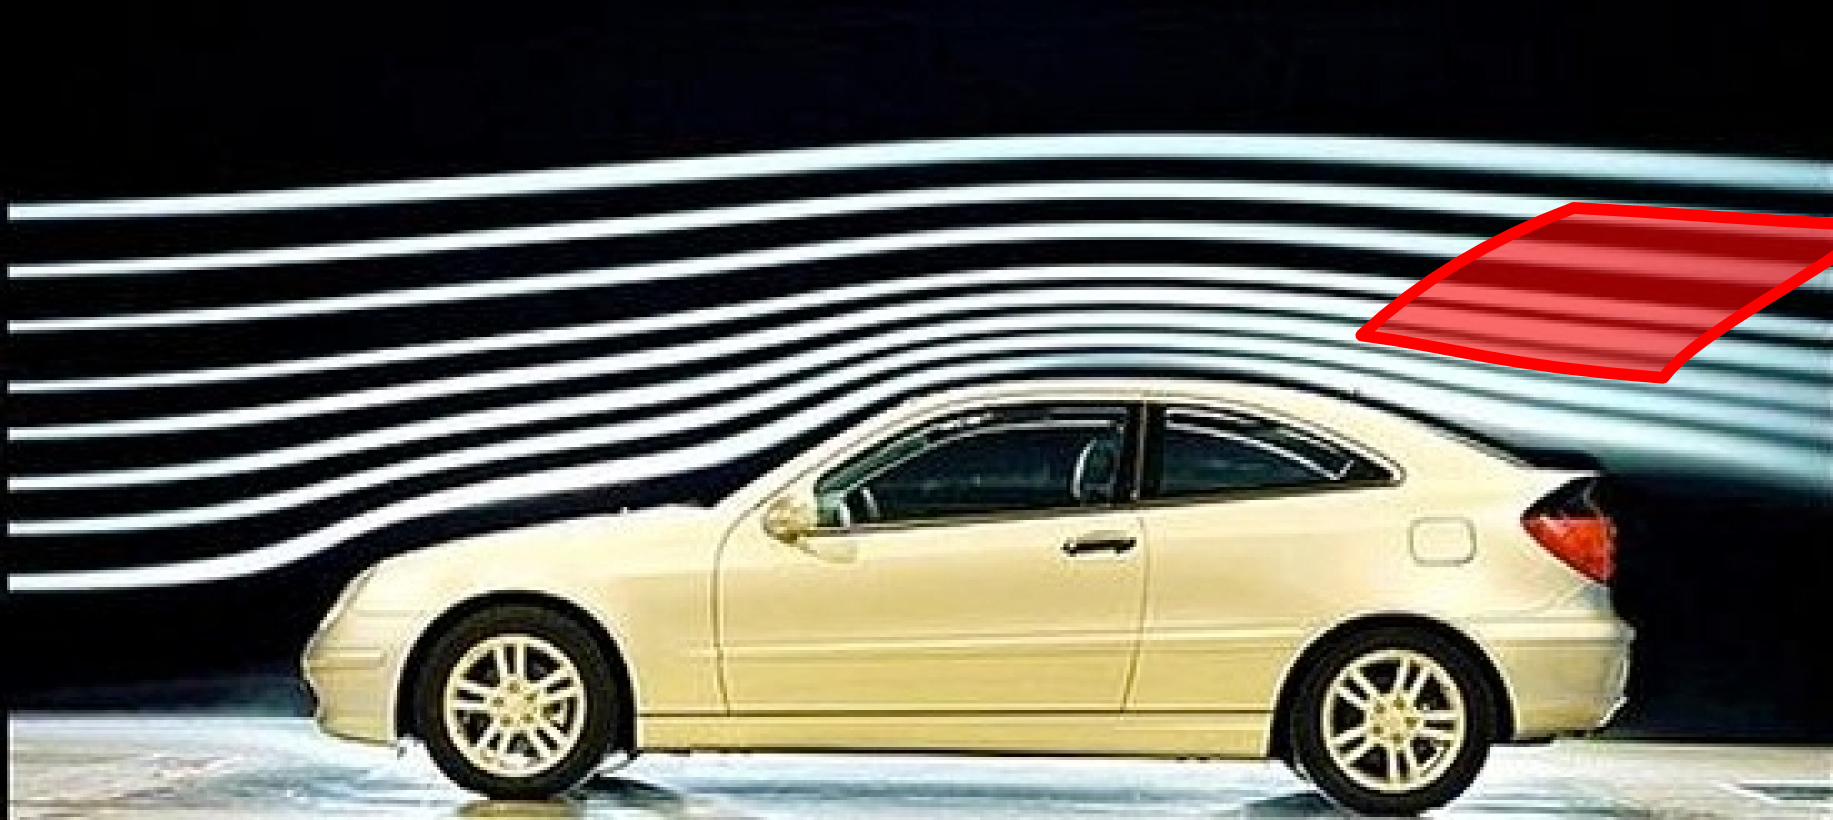
\includegraphics[width=60mm]{volume_materiel6.png}}
\put(22, -5){\color{rouge} Volume matériel $\mathcal{D}(t)$}
\end{picture}
\end{center}

\onslide<9>

\begin{center}
\begin{picture}(60, 35)(0, -5)
\put(0, 0){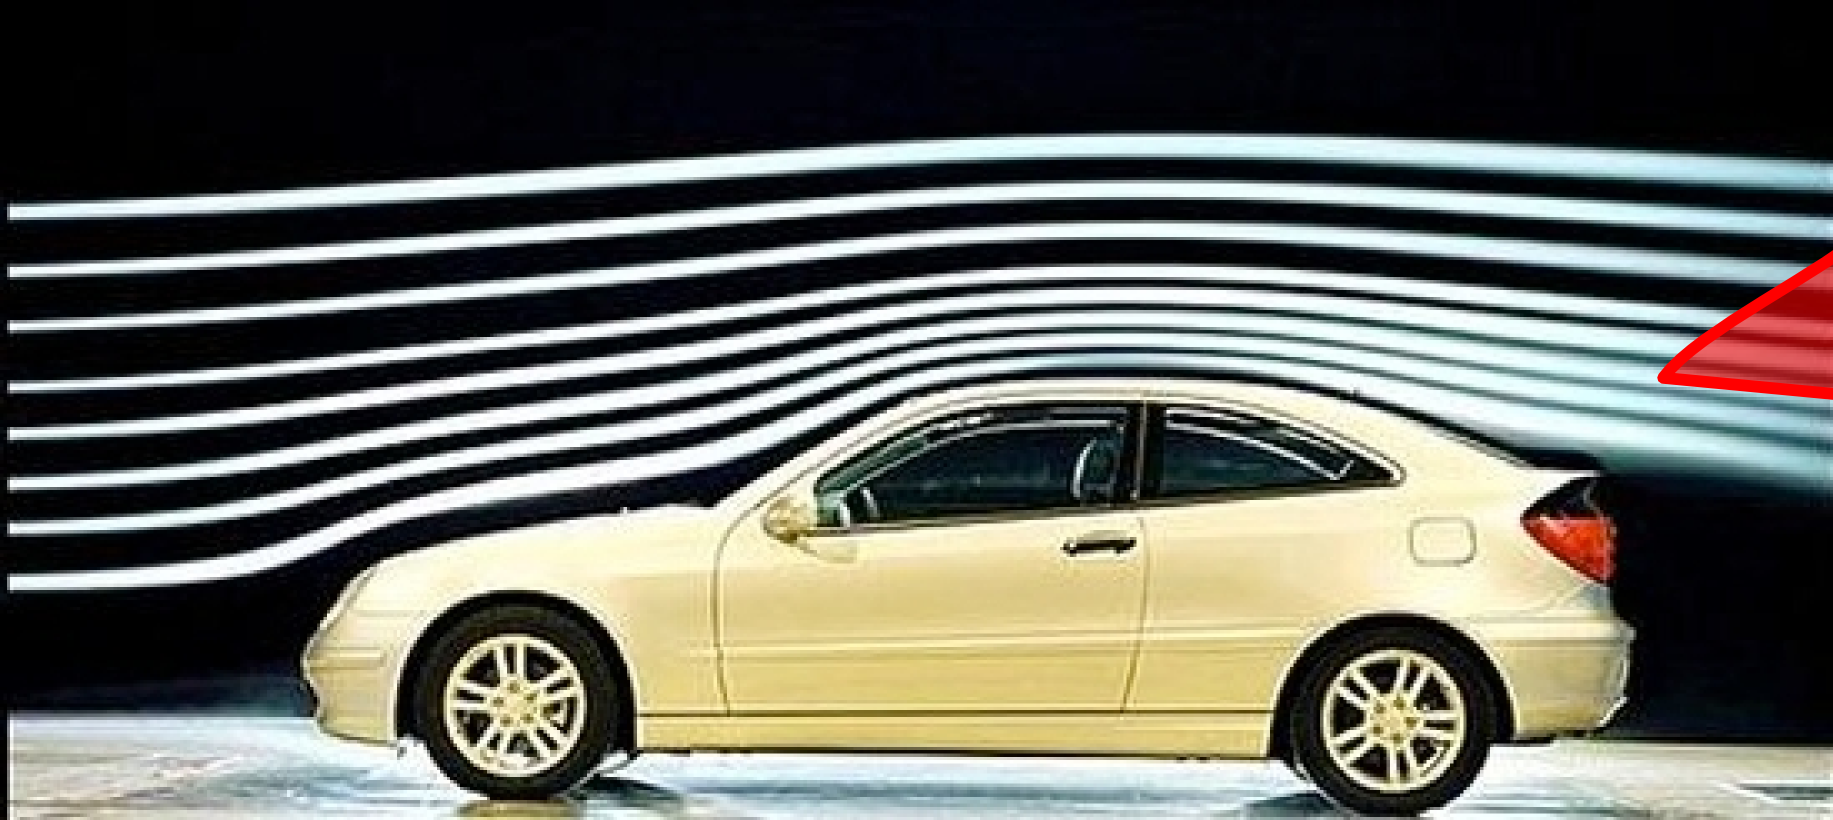
\includegraphics[width=60mm]{volume_materiel7.png}}
\put(22, -5){\color{rouge} Volume matériel $\mathcal{D}(t)$}
\end{picture}
\end{center}

\onslide<10>

\begin{center}
\begin{picture}(60, 35)(0, -5)
\put(0, 0){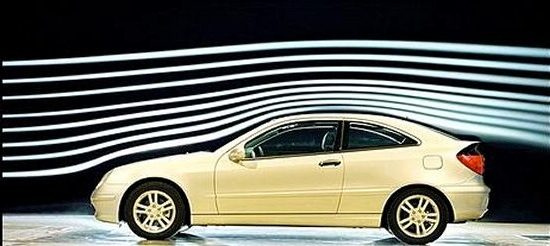
\includegraphics[width=60mm]{streamlines_car.jpg}}
\end{picture}
\end{center}

\onslide<11>

\begin{center}
\begin{picture}(60, 35)(0, -5)
\put(0, 0){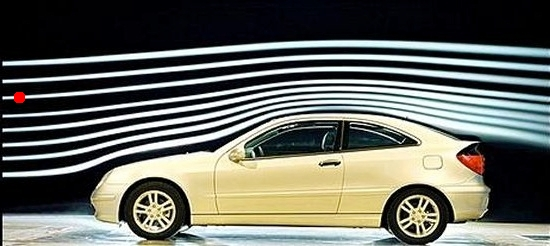
\includegraphics[width=60mm]{streamlines_car1.jpg}}
\put(8, 0.5){\color{bleu} \linethickness{0.5mm} \framebox(46, 24){}}
\put(22, -5){\color{bleu} Volume de contrôle $\Omega$}
\end{picture}
\end{center}

\onslide<12>

\begin{center}
\begin{picture}(60, 35)(0, -5)
\put(0, 0){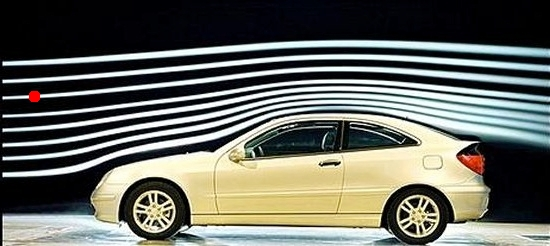
\includegraphics[width=60mm]{streamlines_car2.jpg}}
\put(8, 0.5){\color{bleu} \linethickness{0.5mm} \framebox(46, 24){}}
\put(22, -5){\color{bleu} Volume de contrôle $\Omega$}
\end{picture}
\end{center}

\onslide<13>

\begin{center}
\begin{picture}(60, 35)(0, -5)
\put(0, 0){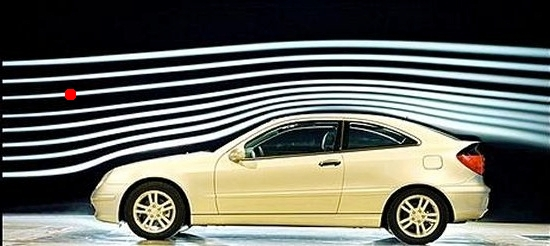
\includegraphics[width=60mm]{streamlines_car3.jpg}}
\put(8, 0.5){\color{bleu} \linethickness{0.5mm} \framebox(46, 24){}}
\put(22, -5){\color{bleu} Volume de contrôle $\Omega$}
\end{picture}
\end{center}

\onslide<14>

\begin{center}
\begin{picture}(60, 35)(0, -5)
\put(0, 0){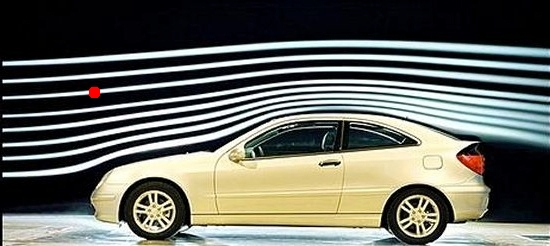
\includegraphics[width=60mm]{streamlines_car4.jpg}}
\put(8, 0.5){\color{bleu} \linethickness{0.5mm} \framebox(46, 24){}}
\put(22, -5){\color{bleu} Volume de contrôle $\Omega$}
\end{picture}
\end{center}

\onslide<15>

\begin{center}
\begin{picture}(60, 35)(0, -5)
\put(0, 0){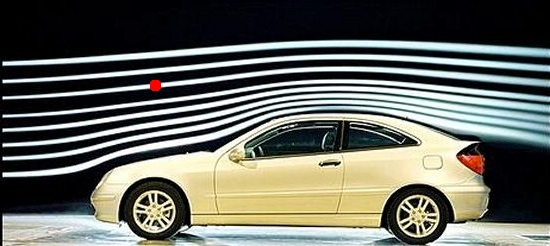
\includegraphics[width=60mm]{streamlines_car5.jpg}}
\put(8, 0.5){\color{bleu} \linethickness{0.5mm} \framebox(46, 24){}}
\put(22, -5){\color{bleu} Volume de contrôle $\Omega$}
\end{picture}
\end{center}

\onslide<16>

\begin{center}
\begin{picture}(60, 35)(0, -5)
\put(0, 0){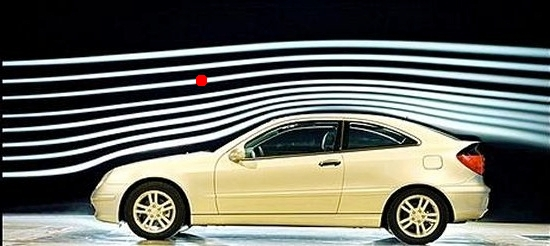
\includegraphics[width=60mm]{streamlines_car6.jpg}}
\put(8, 0.5){\color{bleu} \linethickness{0.5mm} \framebox(46, 24){}}
\put(22, -5){\color{bleu} Volume de contrôle $\Omega$}
\end{picture}
\end{center}

\onslide<17>

\begin{center}
\begin{picture}(60, 35)(0, -5)
\put(0, 0){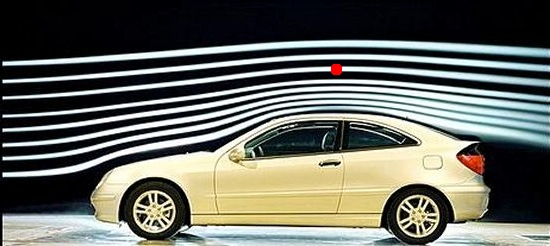
\includegraphics[width=60mm]{streamlines_car7.jpg}}
\put(8, 0.5){\color{bleu} \linethickness{0.5mm} \framebox(46, 24){}}
\put(22, -5){\color{bleu} Volume de contrôle $\Omega$}
\end{picture}
\end{center}

\onslide<18>

\begin{center}
\begin{picture}(60, 35)(0, -5)
\put(0, 0){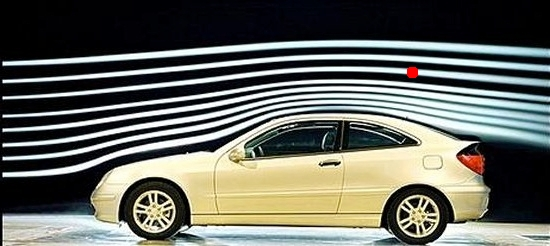
\includegraphics[width=60mm]{streamlines_car8.jpg}}
\put(8, 0.5){\color{bleu} \linethickness{0.5mm} \framebox(46, 24){}}
\put(22, -5){\color{bleu} Volume de contrôle $\Omega$}
\end{picture}
\end{center}

\onslide<19>

\begin{center}
\begin{picture}(60, 35)(0, -5)
\put(0, 0){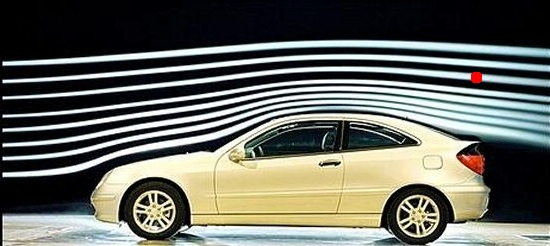
\includegraphics[width=60mm]{streamlines_car9.jpg}}
\put(8, 0.5){\color{bleu} \linethickness{0.5mm} \framebox(46, 24){}}
\put(22, -5){\color{bleu} Volume de contrôle $\Omega$}
\end{picture}
\end{center}

\onslide<20>

\begin{center}
\begin{picture}(60, 35)(0, -5)
\put(0, 0){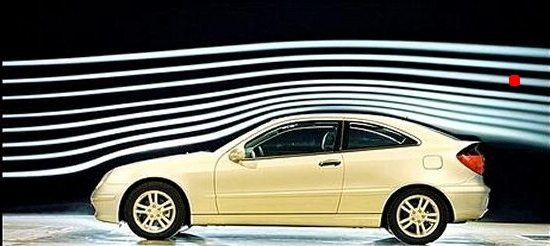
\includegraphics[width=60mm]{streamlines_car10.jpg}}
\put(8, 0.5){\color{bleu} \linethickness{0.5mm} \framebox(46, 24){}}
\put(22, -5){\color{bleu} Volume de contrôle $\Omega$}
\end{picture}
\end{center}

\onslide<21>

\begin{center}
\begin{picture}(60, 35)(0, -5)
\put(0, 0){\includegraphics[width=60mm]{streamlines_car11.jpg}}
\put(8, 0.5){\color{bleu} \linethickness{0.5mm} \framebox(46, 24){}}
\put(22, -5){\color{bleu} Volume de contrôle $\Omega$}
\end{picture}
\end{center}

\end{overprint}

\vspace{5mm}

\end{frame}

%-----------------------------------------------------------------------------------------
\subsubsection{Grandeurs conservatives}
%-----------------------------------------------------------------------------------------
\begin{frame}{Grandeurs conservatives}
%-----------------------------------------------------------------------------------------

\small

\textbf{Définition :}

\medskip

une grandeur est dite \textcolor{vert}{conservative} si $\mydot{F}_p=0$ toujours et partout.


\bigskip 
\pause

\textbf{$\rightarrow$ Théorème :} \medskip

toute grandeur \textcolor{vert}{conservative} associée à un système  \textcolor{vert}{isolé} est \textsl{constante} au cours du temps. 

\bigskip
\pause

\textbf{Exemples :} \medskip

la plupart des grandeurs physiques ne sont pas conservatives, sauf (en mécanique classique) :

\pause

\medskip

\hspace*{5mm}
\begin{minipage}{100mm}
\begin{itemize}[<+-| alert@+>]
\item[$\checkmark$]
	la masse $M$ (sans réaction nucléaire) %: 
%	\qquad $\mydot{M}_p = 0 \qquad \Rightarrow \qquad \ddt{M} = \mydot{M}_e$
\item[$\checkmark$]
	la quantité de mouvement $\myvec{Q}$ %:
%	\qquad $\mydot{\myvec{Q}}_p = 0 \qquad \Rightarrow \qquad \ddt{\myvec{Q}} = \mydot{\myvec{Q}}_e$
\item[$\checkmark$]
	le moment cinétique $\myvec{L}$ %:
%	\qquad $\mydot{\myvec{L}}_p = 0 \qquad \Rightarrow \qquad \ddt{\myvec{L}} = \mydot{\myvec{L}}_e$
\item[$\checkmark$]
	l'énergie totale $E$ %: 
%	\qquad $\mydot{E}_p = 0 \qquad \Rightarrow \qquad \ddt{E} = \mydot{E}_e$
\item[$\checkmark$]
	(la charge électrique )
%	$\color{white}\mydot{E}_p = 0 \Rightarrow \ddt{E} = \mydot{E}_e$  
\end{itemize}
\end{minipage}

\pause 
\medskip

Exemples de grandeurs non conservatives : le volume, l'énergie mécanique, l'énergie interne, l'entropie...

\vspace{0mm}
	
\end{frame}

%-----------------------------------------------------------------------------------------
\subsubsection{Principes de la physique}
%-----------------------------------------------------------------------------------------
\begin{frame}{Principes de la physique}
%-----------------------------------------------------------------------------------------

\small

Les principes de la physique décrivent les échanges avec l'extérieur pour les grandeurs physiques conservatives associées à un système matériel donné :

\bigskip
\pause

\hspace*{5mm}
\begin{minipage}{110mm}
\begin{itemize}[<+-| alert@+>]
\item[$\checkmark$]
	masse : \quad $\mydot{M}_e = 0
	\quad \Rightarrow \quad \color{rouge} \ddt{M} = 0$
\item[$\checkmark$]
	quantité de mouvement : \quad 
	$\mydot{\myvec{Q}}_e = \myvec{F}\indice{ext $\rightarrow \mathcal{D}$}
	\quad \Rightarrow \quad \color{rouge}
	\ddt{\myvec{Q}} = \myvec{F}\indice{ext $\rightarrow \mathcal{D}$}$
\item[$\checkmark$]
	moment cinétique : \quad 
	$\mydot{\myvec{L}}_e = \myvec{\mathcal{M}}\indice{ext $\rightarrow \mathcal{D}$}
	\quad \Rightarrow \quad \color{rouge}
	\ddt{\myvec{L}} = \myvec{\mathcal{M}}\indice{ext $\rightarrow \mathcal{D}$}$
\item[$\checkmark$]
	énergie totale : \quad 
	$\mydot{E}_e = \mathcal{P}\indice{m, ext $\rightarrow \mathcal{D}$} 
	+ \mathcal{P}\indice{th}
		\quad \Rightarrow \quad \color{rouge} 
		\ddt{E} = \mathcal{P}\indice{m, ext $\rightarrow \mathcal{D}$} 
	+ \mathcal{P}\indice{th}$
\item[]
\end{itemize}
\end{minipage}

\vspace{20mm}

\end{frame}


%%==========================================================================================
%\mysubsection{Formes utiles de bilan (à supprimer)}
%%==========================================================================================
%
%%-----------------------------------------------------------------------------------------
%\begin{frame}{Bilan pour un fluide en écoulement}
%%-----------------------------------------------------------------------------------------
%
%\small
%
%\textbf{Objectif :} écrire les équations de bilan pour un écoulement décrit par
%
%\medskip
%
%\begin{itemize}
%\item
%le champ (eulérien) de vitesse $\color{rouge}\myvec{u}(\myvec{x}, t)$ de l'écoulement,
%
%\item
%le champ (eulérien) d'une grandeur conservative $\color{rouge}f(\myvec{x}, t)$ donnée.
%
%\item[]
%Dans le cas où $f$ correspond à une grandeur intensive, on pourra lui associer, pour tout volume $V$ donné, la grandeur extensive $$\color{rouge}\mathcal{F}(t, V) \equiv \int_V f(\myvec{x}, t) \; dV$$ 
%\end{itemize}
%
%\vspace{30mm}
%
%\end{frame}
%
%%-----------------------------------------------------------------------------------------
%\subsubsection{Bilan global}
%%-----------------------------------------------------------------------------------------
%\begin{frame}{Bilan intégral (ou \textsl{global}) : formulation lagrangienne}
%%-----------------------------------------------------------------------------------------
%
%\small
%
%\textbf{Bilan lagrangien :} on considère un \textcolor{vert}{volume matériel} $\mathcal{D}(t)$  
%\mytabbing{\textbf{Bilan lagrangien :}}
%\textcolor{gris}{(on suit la matière dans son mouvement)}
%$$
%	\mathcal{F}(t, \mathcal{D}(t)) = \int_{\mathcal{D}(t)} f(\myvec{x}, t) \; dV
%$$
%
%\begin{picture}(0, 0)(-80, 0)
%	\put(0, 0){\includegraphics[width=25mm]{volume_materiel.png}}
%	\put(0, 1){$\color{red}\mathcal{D}(t)$}
%	\put(-5, 19){$\color{red}\mathcal{D}(t+dt)$}
%\end{picture}
%
%\pause
%
%\begin{itemize}[<+->]
%\item
%	Bilan variationnel :
%	$$
%	d\mathcal{F} 
%	\equiv 
%	\mathcal{F}(t+dt, \mathcal{D}(t+dt)) - \mathcal{F}(t, \mathcal{D}(t)) 
%	= 
%	\delta \mathcal{F}_e
%	$$
%	soit encore :
%	$$ 
%	\int_{\mathcal{D}(t+dt)} f(\myvec{x}, t+dt) \; dV 
%	-
%	\int_{\mathcal{D}(t)} f(\myvec{x}, t) \; dV 
%	= 
%	\mydot{\mathcal{F}}_e dt
%	$$	
%	où $\delta \mathcal{F}_e = \mydot{\mathcal{F}}_e dt$ : quantité échangée avec l'extérieur pendant $dt$.
%	\medskip
%\item 
%	Equation d'évolution : 
%	
%	\smallskip
%	
%	en divisant par $dt \rightarrow 0$ l'expression précédente, on obtient
%	
%	\smallskip
%	
%	\begin{equation}
%	\mydot{\mathcal{F}} \equiv \ddt{\mathcal{F}} 
%	= \color{rouge}
%	\ddt{} \int_{\mathcal{D}(t)} f(\myvec{x}, t) \; dV
%	=
%	\mydot{\mathcal{F}}_e
%	\label{eq:bilan_global_lagrangien}
%	\end{equation}
%\end{itemize}
%
%\vspace{5mm}
%
%\end{frame}
%
%
%%-----------------------------------------------------------------------------------------
%\begin{frame}{Bilan intégral (ou \textsl{global}) : formulation eulérienne}
%%-----------------------------------------------------------------------------------------
%
%\small
%
%
%\textbf{Bilan eulérien :} on considère un \textcolor{vert}{volume de contrôle} fixe $\Omega$,
%\mytabbing{\textbf{Bilan eulérien :}} 
%de frontière $\partial \Omega$ et de normale sortante $\myvec{n}$.
%
%\medskip
%
%Soit $\mathcal{D}(t)$
%le volume matériel coïncidant avec $\Omega$ à l'instant $t$ :
%
%\begin{picture}(0, 0)(-80, 5)
%	\put(0, 0){\includegraphics[width=25mm]{volumes.png}}
%	\put(0, 1){$\color{red}\mathcal{D}(t)$}
%	\put(22, 1){$\color{blue}\Omega$}
%	\put(-5, 19){$\color{red}\mathcal{D}(t+dt)$}
%\end{picture}
%
%\pause
%
%\vspace{-1mm}
%
%\begin{itemize}[<+->]
%\item
%	Par le théorème de transport de Reynolds, \\ l'équation d'évolution précédente s'écrit :
%	$$
%	\ddt{} \int_{\mathcal{D}(t)} f(\myvec{x}, t) \; dV 
%	=
%	\mydot{\mathcal{F}}_e
%	\quad \Rightarrow \quad
%	\dpdt{} \int_{\Omega} f(\myvec{x}, t) \; dV 
%	+ 
%	\oint_{\partial \Omega} f(\myvec{x}, t) \myvec{u}(\myvec{x}, t)\cdot \myvec{n} \, dS
%	=
%	\mydot{\mathcal{F}}_e
%	$$
%	soit
%	\begin{equation} \color{rouge}
%	\dpdt{} \int_{\Omega} f(\myvec{x}, t) \; dV 
%	=
%	\mydot{\mathcal{F}}_e
%	- \oint_{\partial \Omega} f(\myvec{x}, t) \;  \myvec{u}(\myvec{x}, t)\cdot \myvec{n} \, dS
%	\label{eq:bilan_global_eulerien}
%	\end{equation}
%	
%Le dernier terme s'interprète comme un terme supplémentaire d'échange ou de flux, 
%\\
%dit \textsl{advectif}, lié à la traversée de la frontière $\partial \Omega$ 
%du \textcolor{vert}{système ouvert} $\Omega$ par des particules matérielles transportant avec elles
%la quantité $f$. 
%
%\medskip
%
%\item
%	Cette équation d'évolution peut aussi s'écrire sous la forme d'un bilan variationnel 
%	\begin{eqnarray*}
%		d\mathcal{F} & = &  \mathcal{F}(t+dt, \Omega) - \mathcal{F}(t, \Omega)
%		\\ & =& 
%		 \int_\Omega f(\myvec{x}, t+dt) \; dV - \int_\Omega f(\myvec{x}, t) \; dV
% =		\mydot{\mathcal{F}}_e dt
%	 	- \left (
%		\oint_{\partial \Omega} f(\myvec{x}, t) \;  \myvec{u}(\myvec{x}, t)\cdot \myvec{n} \, dS
%		\right ) \, dt
%	\end{eqnarray*}
%	où le dernier terme correspond à la quantité $f$ échangée 
%	pendant $dt$ par flux de matière à travers la frontière $\partial \Omega$.
%\end{itemize}
%
%\vspace{0mm}
%
%\end{frame}
%
%%\end{document}
%
%%-----------------------------------------------------------------------------------------
%\subsubsection{Bilan local}
%%-----------------------------------------------------------------------------------------
%\begin{frame}{Bilan local (ou \textsl{différentiel})}
%%-----------------------------------------------------------------------------------------
%
%\small
%
%\textbf{Objectif :} 
%
%\begin{center}
%application des bilans intégraux précédents sur un volume \textcolor{vert}{infinitésimal}
%$v \rightarrow 0$ :
%
%\medskip
%
%$$
%\mathcal{F}(t, v) = \int_v \, f(\myvec{x}, t) \; dV \approx f(\myvec{x}, t) \, v
%$$
%
%\bigskip
%
%\begin{picture}(0, 10)
% \put(0, 10){\vector(0, -1){10}}
%\end{picture}
%
%\bigskip
%
%dérivation des équations aux dérivées partielles
%
%correspondant aux bilans locaux ainsi obtenus
%
%\end{center}
%
%\vspace{20mm}
%
%\end{frame}
%
%%-----------------------------------------------------------------------------------------
%\begin{frame}{Bilans locaux lagrangien et eulérien}
%%-----------------------------------------------------------------------------------------
% 
%\small
%
%\textbf{Bilan lagrangien :}
%
%\medskip
%
%En notant $\mydot{f}_e$ le taux d'échange par unité de volume, 
%la loi d'évolution lagrangienne pour le volume matériel
%$\mathcal{D}(t)$ obtenue précédemment s'écrit :
%	$$ 
%	\ddt{} \int_{\mathcal{D}(t)} f(\myvec{x}, t) \; dV
%	=
%	\mydot{\mathcal{F}}_e
%	= \int_{\mathcal{D}(t)} \mydot{f}_e \; dV
%	$$ 
%\pause
%Si $\mathcal{D}(t)$ correspond à un volume matériel infinitésimal $v$ :
%$$
%\ddt{} \left (f v \right) = \mydot{f}_e v 
%\quad \Rightarrow \quad
%\ddt{f} v + f \ddt{v} = \mydot{f}_e v 
%\quad \Rightarrow \quad
%\ddt{f} + f \frac{1}{v} \ddt{v}= \mydot{f}_e
%\quad \mbox{avec} \quad \dfrac{1}{v} \ddt{v} = \divergence \myvec{u}
%$$
%\pause
%On en déduit l'équation locale 
%en suivant la particule fluide dans son mouvement :
%\begin{equation}
%	\color{rouge}
%	\ddt{f} + f\divergence \myvec{u} = \mydot{f}_e
%	\label{eq:bilan_local_lagrangien}
%\end{equation}
%
%\pause
%\textbf{Bilan eulérien :}
%
%\medskip
%
%En remarquant que 
%$
%	\ddt{f} + f\divergence \myvec{u} 
%	= 
%	( \dpdt{f} + {\color{vert}\myvec{u} \cdot \gradient f } ) + {\color{vert} f\divergence \myvec{u}}
%	= 
%	\dpdt{f} + {\color{vert} \divergence ( f\myvec{u})},
%$
%\pause
%on en déduit l'équation locale :
%\begin{equation}
%	\color{rouge}
%	\dpdt{f} + \divergence ( f\myvec{u}) = \mydot{f}_e
%	\label{eq:bilan_local_eulerien}
%\end{equation}
%
%\medskip
%\pause
%
%\textcolor{vert}{\sl Exercice :} retrouver cette équation locale en écrivant le bilan intégral en formulation eulérienne (\ref{eq:bilan_global_eulerien})
%\mytabbing{\sl Exercice :} sur un volume de contrôle infinitésimal fixe $dx \times dy \times dz$.
%
%\end{frame}
%
 
%==========================================================================================
\subsection{Bilan de masse}
%==========================================================================================

%-----------------------------------------------------------------------------------------
\subsubsection{bilans intégraux}
%-----------------------------------------------------------------------------------------
\begin{frame}{Bilan de masse : bilans intégraux}
%-----------------------------------------------------------------------------------------

\small


Quantité physique : \textbf{masse} $M$ associée à la grandeur intensive $\rho$ (\textbf{masse volumique}).

\bigskip

Pour un volume matériel $\mathcal{D}(t)$ donné 
$$
	M(t, \mathcal{D}) = \int_{\mathcal{D}(t)} \rho(\myvec{x}, t) \, dV
$$

\medskip 

\pause

Pour ce système matériel, le principe de conservation de la masse $\ddt{M} = 0$ s'écrit :

\medskip

\begin{itemize}
\item
	Bilan global lagrangien pour le volume matériel $\mathcal{D}$ en suivant le fluide
	dans son mouvement
	\begin{equation}
		\color{rouge}
		\ddt{} \int_{\mathcal{D}(t)} \rho(\myvec{x}, t) \; dV 
		= 0
		\label{eq:bilan_global_lagrangien_masse}
	\end{equation}
\medskip

\pause

\item
  Bilan global eulérien pour le volume de contrôle fixe $\Omega$ (système ouvert)
	\begin{equation}
		\mbox{\textcolor{gris}{[Démonstration] \quad $\longrightarrow$ \quad}}
		\color{rouge}
		\dpdt{} \int_{\Omega} \rho(\myvec{x}, t) \; dV 
		=
		- \oint_{\partial \Omega} \rho \,  \myvec{u}\cdot \myvec{n} \, dS
		\label{eq:bilan_global_eulerien_masse}
	\end{equation}
\end{itemize}

\pause
\medskip

%\hfill 
\textcolor{vert}{Exemples d'application :}

\pause

Conservation du débit massique dans une canalisation.

Ecoulement à travers un évaporateur.

Cocotte-minute

(...)


%\quad \textcolor{gris}{[Démonstration]}

\vspace{0mm}

\end{frame}

%-----------------------------------------------------------------------------------------
\subsubsection{bilans locaux}
%-----------------------------------------------------------------------------------------
\begin{frame}{Bilan de masse : bilans locaux}
%-----------------------------------------------------------------------------------------

\small

A partir des bilans intégraux précédents, on déduit les équations locales de bilan de masse :

\medskip

\begin{itemize}

\item
  Bilan local eulérien
	\begin{equation}
			\color{rouge}
		\dpdt{\rho} + \divergence ( \rho \, \myvec{u}\ ) = 0
		\label{eq:bilan_local_eulerien_masse}
	\end{equation}
\medskip

\pause 
\textcolor{gris}{[Démonstrations :]}

\begin{itemize}
	\item $(i)$ A partir du bilan intégral Eulérien, à l'aide du théorème de la divergence
	\item $(ii)$ Directement par un bilan sur un volume élémentaire 
\end{itemize}


\pause

\item
	Bilan local lagrangien, en suivant la particule fluide dans son mouvement
	\begin{equation}
		\color{rouge}
		\ddt{\rho} + \rho \, \divergence \myvec{u} = 0
		\label{eq:bilan_local_lagrangien_masse}
	\end{equation}
\pause

\textcolor{gris}{[Démonstrations :] }
\begin{itemize}
	\item $(i)$ En utilisant la définition de la dérivée particulaire
	\item $(ii)$ En variables lagrangiennes (cf. MMC) 
\end{itemize}


\end{itemize}
\end{frame}

%-----------------------------------------------------------------------------------------
\begin{frame}{Ecoulement incompressible}
%-----------------------------------------------------------------------------------------

\small



Conséquences du bilan local de masse :

$$
\ddt{\rho} + \rho \, \divergence \myvec{u} = 0
$$

Si $\rho$ est constante sur chaque ligne de courant ($\ddt{\rho} = 0$),
alors l'écoulement est à divergence nulle.

\medskip
\pause 
On parle d'{\em écoulements isovolumes} ou (par abus de language)
d'{\em écoulements incompressibles}.

\medskip 
\pause 
Classe d'écoulements très importante...


\medskip 
\pause 
Cette hypothèse  est justifiée :

\begin{itemize}
\item Dans les liquides pour des raisons thermodynamiques 
(les liquides sont très faiblement compressibles)

\item Dans les gaz (fluides compressibles du point de vue thermo) si la vitesse de l'écoulement est faible devant la {\em vitesse du son } $c$ définie par

$$
c^2 
= \left(\frac{\partial p}{\partial \rho} \right)_s = \frac{1}{\rho \chi_s} = 
\sqrt{\gamma r T}
$$

(Remarque : $c^2  \approx v_q^2$ ; cf. chap. 1)
\end{itemize}

\pause 
Cette hypothèse s'écrit aussi : 
$$ 
M =\frac{U}{c} \ll 1
$$

(justification : cf. chapitre 10)

\end{frame}


% 
%
%
%
%On considère ici un \textbf{écoulement incompressible}
%(ou plus exactement \textsl{isovolume}) c'est-à-dire pour lequel les conditions sont telles que le volume $v$ de chaque particule fluide peut \^etre consid\'er\'e comme constant au cours du temps.
%
%\medskip
%\pause
%
%Cette hypothèse se traduit par l'\'equation dite \textsl{de continuit\'e} :
%\begin{equation}
%  \frac{1}{v} \ddt{v} = 0 
%  \quad \Rightarrow \quad
%  \color{rouge} \divergence \myvec{u} = 0
%  \label{eq:incompressibilite}
%\end{equation}
%
%\medskip
%\pause
%Dans ces conditions, l'\'equation de conservation de la masse s'\'ecrit :
%\begin{equation}
%  \ddt{\rho} + \rho \; \divergence{\myvec{u}} = 0
%  \quad \Rightarrow \quad
%  \color{rouge} \ddt{\rho} = 0
%\end{equation}
%ce qui s'interprète physiquement par le fait que la masse volumique est conserv\'ee 
%lorsque l'on suit les particules fluides dans leur mouvement (et donc 
%la masse volumique de chaque particule fluide reste constante au cours du temps).
%
%\pause
%\vspace{10mm}
%
%Ce r\'esultat est bien s\^ur coh\'erent avec l'hypoth\`ese d'\'ecoulement 
%isovolume et le principe de conservation de la masse 
%appliqu\'e \`a chaque particule fluide \textcolor{gris}{[Démonstration]}.
%
%\vspace{10mm}
%
%\end{frame}
%


%\vspace{20mm}

%\end{frame}

%==========================================================================================
\subsection{Bilan de quantité de mouvement}
%==========================================================================================

%-----------------------------------------------------------------------------------------
\subsubsection{Bilans intégraux}
%-----------------------------------------------------------------------------------------
\begin{frame}{Bilan de quantité de mouvement : bilans intégraux}
%-----------------------------------------------------------------------------------------

\small

Quantité physique : quantité de mouvement $\myvec{Q}$ associée à la grandeur intensive 
$\rho \, \myvec{u}$.

\medskip

Pour un volume matériel $\mathcal{D}(t)$ donné : 
$ \displaystyle
	\myvec{Q}(t, \mathcal{D}) 
	= \int_{\mathcal{D}(t)} \rho(\myvec{x}, t)\, \myvec{u}(\myvec{x}, t) \, dV
$

\pause

Principe de conservation de la quantité de mouvement : 
$\ddt{\myvec{Q}} = \myvec{F}\indice{ext $\rightarrow \mathcal{D}$}$

\smallskip

\begin{itemize}
\item
	Bilan global lagrangien pour le volume matériel $\mathcal{D}$ en suivant le fluide
	dans son mouvement
	\begin{equation}
		\color{rouge}
		\ddt{} \int_{\mathcal{D}(t)} \rho \, \myvec{u} \; dV 
		=
		\int_{\mathcal{D}(t)} \rho \myvec{f} \, dV 
		+ \oint_{\partial \mathcal{D}(t)} 
		\left( -p \myvec{n} + \mytensor{\tau} \cdot \myvec{n}\right) \; dS
		\label{eq:bilan_global_lagrangien_qdm}
	\end{equation}
	où $\myvec{f}$ désigne toute force à distance par unité de masse (ex. gravité $\myvec{g}\ $)
	
	et où les forces surfaciques sont la pression (normale) et la contrainte visqueuse (représentée par le tenseur $\mytensor{\tau}$).
	Ce bilan s'interprète simplement comme le \textcolor{vert}{principe fondamental de la dynamique} 
	appliqué au système matériel $\mathcal{D}$.

\smallskip

\pause
\item
  Bilan global eulérien pour le volume de contrôle fixe $\Omega$ (système ouvert)
	\begin{equation}
		\hspace*{-11mm} \mbox{\color{gris} [Démonstration] \; $\longrightarrow$ \;}  
		\color{rouge}
		\dpdt{} \int_{\Omega} \rho \, \myvec{u} \; dV 
		=
		\int_{\Omega} \rho \myvec{f} \, dV 
		+ \oint_{\partial \Omega} \left( -p \myvec{n} + \mytensor{\tau} \cdot \myvec{n}\right) \; dS
		- \oint_{\partial \Omega} \rho \, \myvec{u}\; (\myvec{u}\cdot \myvec{n}) \, dS
		\label{eq:bilan_global_eulerien_qdm}
	\end{equation}
\end{itemize}

\pause

Remarque : en présence d'interface traversant la frontière du volume considéré, il faut ajouter au membre de droite la contribution de la force de tension superficielle
$$
\int_{\mathcal{L}} \gamma \myvec{\tau} \, dl
$$

%\vspace{0mm}

\end{frame}
%-----------------------------------------------------------------------------------------
\subsubsection{Bilans locaux}
%%-----------------------------------------------------------------------------------------
%\begin{frame}{Bilan de quantité de mouvement : bilans locaux}
%%-----------------------------------------------------------------------------------------
%
%\small
%
%En utilisant le théorème de la divergence sur le bilan intégral lagrangien, et en écrivant ce bilan
%pour un volume matériel infinitésimal $dV$, de masse $dm = \rho dV$, 
%on déduit les équations locales de bilan de quantité de mouvement :
%
%\medskip
%\pause
%
%\begin{itemize}
%\item
%	Bilan local lagrangien, en suivant la particule fluide dans son mouvement :
%	\begin{equation}
%		\mbox{\textcolor{gris}{[Démonstration] \quad $\longrightarrow$ \quad}}
%		\rho \ddt{\myvec{u}} 
%		= 
%		\rho \myvec{f} + \divergence \mytensor{\sigma}
%		%\label{eq:bilan_local_lagrangien_qdm}
%	\end{equation}
%	
%	\medskip
%	En multipliant par le volume de la particule fluide, ce bilan local s'interprète comme
%	\\ le \textcolor{vert}{principe fondamental de la dynamique} appliqué à la particule fluide.
%
%	\pause
%
%	\bigskip
%	En écrivant que pour un fluide $\mytensor{\sigma} = -p \mytensor{1} + \mytensor{\tau}$,
%	le bilan local donne l'équation de Navier-Stokes généralisée :
%	\begin{equation}
%		\color{rouge}
%		\rho \ddt{\myvec{u}} 
%		= 
%		\rho \myvec{f} - \gradient p + \divergence \mytensor{\tau}
%		\label{eq:bilan_local_lagrangien_qdm}
%	\end{equation}
%
%\bigskip
%\pause
%
%\item
%  Bilan local eulérien : on déduit directement de l'expression précédente
%	\begin{equation}
%		\rho \left [ \dpdt{\myvec{u}} + \left ( \myvec{u} \cdot \gradient\ \right ) \myvec{u} \right ]
%		= \rho \myvec{f} + \divergence \mytensor{\sigma}
%		%\label{eq:bilan_local_eulerien_qdm}
%	\end{equation}
%	ou encore
%	\begin{equation}
%		\color{rouge}
%		\rho \left [ \dpdt{\myvec{u}} + \left ( \myvec{u} \cdot \gradient\ \right ) \myvec{u} \right ]
%		= \rho \myvec{f} - \gradient p + \divergence \mytensor{\tau}
%		\label{eq:bilan_local_eulerien_qdm}
%	\end{equation}
%\end{itemize}
%
%
%\vspace{15mm}
%
%\end{frame}

%-----------------------------------------------------------------------------------------
\subsubsection{Bilans locaux}
%-----------------------------------------------------------------------------------------
\begin{frame}{Bilan de quantité de mouvement : bilans locaux}
%-----------------------------------------------------------------------------------------

\small

%En utilisant le théorème de la divergence sur le bilan intégral lagrangien, et en écrivant ce bilan
%pour un volume matériel infinitésimal $dV$, de masse $dm = \rho dV$, 
%on déduit les équations locales de bilan de quantité de mouvement :

\medskip
\pause

\begin{itemize}
\item
  Bilan local eulérien 
	%\begin{equation}
	%	\rho \left [ \dpdt{\myvec{u}} + \left ( \myvec{u} \cdot \gradient\ \right ) \myvec{u} \right ]
	%	= \rho \myvec{f} + \divergence \mytensor{\sigma}
		%\label{eq:bilan_local_eulerien_qdm}
	%\end{equation}
	%ou encore
	\begin{equation}
		\color{rouge}
		\rho \left [ \dpdt{\myvec{u}} +  \mytensor{grad}(\myvec{u}) \cdot \myvec{u} \right ]
		= \rho \myvec{f} - \gradient p + \divergence \mytensor{\tau}
		\label{eq:bilan_local_eulerien_qdm}
	\end{equation}


Démo : a partir du bilan global  Eulérien, à l'aide du théorème de la divergence.


\item
	Bilan local lagrangien, 
	\begin{equation}
		\mbox{\textcolor{gris}{[Démonstration] \quad $\longrightarrow$ \quad}}
		\rho \ddt{\myvec{u}} 
		= 
		\rho \myvec{f}  - \gradient p + \divergence \mytensor{\tau}
		%\label{eq:bilan_local_lagrangien_qdm}
	\end{equation}
	
	\medskip
	Ce bilan local s'interprète comme
	\\ le \textcolor{vert}{principe fondamental de la dynamique} appliqué à la particule fluide.

	\pause

	
\bigskip
\pause

\end{itemize}


\vspace{15mm}

\end{frame}

%==========================================================================================
\subsection{Bilans d'énergie}
%==========================================================================================

%-----------------------------------------------------------------------------------------
\begin{frame}{Bilans d'énergie}
%-----------------------------------------------------------------------------------------

\small

$\rightarrow$ cf. cours de Transferts thermiques (à traiter à titre d'exercice).

\vspace{40mm}

\end{frame}

%==========================================================================================
\subsection{Equation de Navier--Stokes}
%==========================================================================================
%
%%-----------------------------------------------------------------------------------------
%\subsubsection{Ecoulement incompressible de fluide newtonien}
%%-----------------------------------------------------------------------------------------
%\begin{frame}{Ecoulement incompressible}
%%-----------------------------------------------------------------------------------------
%
%\small
%
%On considère ici un \textbf{écoulement incompressible}
%(ou plus exactement \textsl{isovolume}) c'est-à-dire pour lequel les conditions sont telles que le volume $v$ de chaque particule fluide peut \^etre consid\'er\'e comme constant au cours du temps.
%
%\medskip
%\pause
%
%Cette hypothèse se traduit par l'\'equation dite \textsl{de continuit\'e} :
%\begin{equation}
%  \frac{1}{v} \ddt{v} = 0 
%  \quad \Rightarrow \quad
%  \color{rouge} \divergence \myvec{u} = 0
%  \label{eq:incompressibilite}
%\end{equation}
%
%\medskip
%\pause
%Dans ces conditions, l'\'equation de conservation de la masse s'\'ecrit :
%\begin{equation}
%  \ddt{\rho} + \rho \; \divergence{\myvec{u}} = 0
%  \quad \Rightarrow \quad
%  \color{rouge} \ddt{\rho} = 0
%\end{equation}
%ce qui s'interprète physiquement par le fait que la masse volumique est conserv\'ee 
%lorsque l'on suit les particules fluides dans leur mouvement (et donc 
%la masse volumique de chaque particule fluide reste constante au cours du temps).
%
%\pause
%\vspace{10mm}
%
%Ce r\'esultat est bien s\^ur coh\'erent avec l'hypoth\`ese d'\'ecoulement 
%isovolume et le principe de conservation de la masse 
%appliqu\'e \`a chaque particule fluide \textcolor{gris}{[Démonstration]}.
%
%\vspace{10mm}
%
%\end{frame}

%\end{document}


%\begin{frame}{Loi rhéologique pour un fluide Newtonien (complément chap. 2)}



%On a vu au chap. 2 que la viscosité est la manifestation d'une force  

%se place dans le cas d'un \textbf{fluide newtonien}, c'est à dire : 

%Les contraintes sont des fonctions linéaires des taux de déformation.

%(cf. chapitre 2 pour un écoulement parallèle : $\tau_{xy} = \mu \partial v/\partial x$)

%\end{frame}

%\end{document}


\begin{frame}{Ecoulement incompressible de fluide newtonien}
%-----------------------------------------------------------------------------------------

\small

Dans le cas général, le bilan de quantité de mouvement pour un fluide en écoulement s'écrit
\begin{equation}
	\color{rouge}
	\rho \ddt{\myvec{u}} 
	= \rho \myvec{f} + \divergence \mytensor{\sigma}
	= \rho \myvec{f} - \gradient p + \divergence \mytensor{\tau}
	\label{eq:Cauchy}
\end{equation}

\pause

On se place dans le cas d'un \textbf{fluide newtonien}, c'est-à-dire dont le tenseur des contraintes
visqueuses $\mytensor{\tau}$ est donné par la loi de comportement, dite de Newton,
\[
	\mytensor{\tau} = 2 \mu \, \mytensor{D}
\] 

où $\mu$ désigne la viscosité dynamique du fluide et le tenseur des taux de déformations est donné par
\[
	\mytensor{D} = \frac{1}{2}\, \left ( \ggradient\ \myvec{u} + \,^t\ggradient\ \myvec{u} \right )
\] 

\pause
Dans ces conditions, et sous réserve que la viscosité dynamique $\mu$ est uniforme, on montre que
\[
	\divergence \mytensor{\tau} = \mu\, \Delta \myvec{u}
	\hspace{10mm} \mbox{\color{gris} [Exercice]}
\]
\pause
et l'équation (\ref{eq:Cauchy}) s'écrit alors
\begin{equation*}
	\color{rouge}
	\frac{d\myvec{u}}{dt} 
	=
	\myvec{f}
	-
	\frac{1}{\rho} \, \gradient p
	+
	\nu \, \Delta \myvec{u} 
\end{equation*}

\vspace{5mm}

\end{frame}


%-----------------------------------------------------------------------------------------
\begin{frame}{Equation de Navier--Stokes}
%-----------------------------------------------------------------------------------------

\small

L'équation précédente s'écrit aussi, en explicitant la dérivée particulaire :
\begin{equation}
	\color{rouge}
	\frac{d\myvec{u}}{dt} 
	= 
	\dpdt{\myvec{u}} + \left ( \myvec{u} \cdot \gradient \right )\myvec{u}
	=
	\myvec{f}
	-
	\frac{1}{\rho} \, \gradient p
	+
	\nu \, \Delta \myvec{u} 
	\label{eq:Navier-Stokes}
\end{equation}


Il s'agit de l'équation de \textcolor{vert}{Navier--Stokes} pour l'écoulement 
\textsl{incompressible} 
d'un fluide \textsl{newtonien}, de viscosité cinématique \textsl{uniforme} $\nu = \mu/\rho$.

\pause
\medskip

Cette équation est à coupler avec l'équation (\ref{eq:incompressibilite}) $\color{rouge} \divergence{\myvec{u}} = 0$ et, dans le cas d'un fluide \textbf{homogène} 
(\textit{i.e.} de masse volumique $\rho$ uniforme), 
on obtient alors un système de quatre équations aux dérivées partielles en temps et en espace
pour les quatre inconnues $(\myvec{u}, p)$.

\medskip

A ce système différentiel on doit adjoindre des \textcolor{vert}{conditions initiales} (en temps)
et des \textcolor{vert}{conditions aux limites} (en espace) du domaine fluide étudié. 

\medskip
\pause

L'équation de Navier--Stokes est une équation fondamentale en mécanique des fluides 
en particulier, et en physique en général. 
Elle se caractérise par une forte complexité liée aux termes non linéaires
$\color{rouge} \left ( \myvec{u} \cdot \gradient \right )\myvec{u}$, qui autorisent 
la co-existence de plusieurs
solutions possibles, pour des mêmes conditions d'écoulement.
La difficulté est alors double : d'une part déterminer les écoulements solutions possibles 
des équations et, d'autre part, de prédire lequel de ces écoulements solutions 
sera effectivement sélectionné et donc observé dans la réalité. 
Ce dernier point est directement lié aux propriétés de stabilité 
des différents écoulements solutions.

\medskip

Bien que connue depuis le milieu du XIXème siècle, cette équation reste paradoxalement 
mal comprise et maîtrisée à ce jour. 
A ce titre son étude est au c{\oe}ur de nombreuses recherches actuelles, et 
sa résolution constitue l'un des dix grands défis de la physique moderne 
(et fait accessoirement l'objet d'un prix d'un million de dollars, 
pour ceux que cela intéresse\ldots). 

\vspace{0mm}

\end{frame}

%-----------------------------------------------------------------------------------------
\subsubsection{Conditions aux limites}
%-----------------------------------------------------------------------------------------
\begin{frame}{Conditions aux limites : condition cinématique}
%-----------------------------------------------------------------------------------------

\small
Pour que la mise en équation du paragraphe précédent soit mathématiquement bien posée, \\
il faut compléter les équations aux dérivées partielles (\ref{eq:incompressibilite})
et (\ref{eq:Navier-Stokes}) par des \textcolor{vert}{conditions aux limites} \\
décrivant ce qui se passe physiquement aux frontières du domaine fluide étudié.

\smallskip

Ces conditions sont de deux types. 

\smallskip
\pause

Le premier type de condition limite, dite \textsl{\color{vert}condition cinématique}, 
traduit la continuité à chaque instant de la vitesse entre le fluide 
et le milieu extérieur à la traversée de la frontière $\Sigma$ du domaine~:
\begin{equation}
	\color{rouge}
	\myvec{u}(\myvec{x} \in \Sigma, t) = \myvec{u}\indice{ext}(\myvec{x} \in \Sigma, t)
	\label{eq:condition cinematique}
\end{equation}
où $\myvec{u}$ et $\myvec{u}\indice{ext}$ désignent respectivement la vitesse du fluide et celle du milieu
extérieur.

\smallskip

Cette condition, qui n'est pas évidente en soi et qui a mis du temps à s'imposer historiquement, 
est effectivement bien vérifiée expérimentalement pour la plupart des écoulements de fluides visqueux
dans conditions opérationnelles (thermodynamiques notamment) standards.

	\begin{center}
		\setlength{\unitlength}{0.7mm}
		\begin{picture}(90, 50)
			\put(0, 0){\includegraphics[width=63mm]{conditions_limites.png}}	
			\put(58, 39){$\myvec{n}$}
			\put(63.5, 32){milieu extérieur}
			\put(63, 27){(fluide ou solide)}
			\put(28, 17){\setlength{\fboxsep}{1mm}\colorbox{white}{$\myvec{x}$}} 
			\put(9, 24){frontière $\Sigma$}
			\put(63, 15){fluide}
		\end{picture}
	\end{center}


\vspace{0mm}

\end{frame}

%-----------------------------------------------------------------------------------------
\begin{frame}{Conditions aux limites : condition dynamique}
%-----------------------------------------------------------------------------------------

\small

Le second type de condition limite, dite \textsl{\color{vert}condition dynamique},  
exprime l'équilibre mécanique de \\
la frontière, qui se traduit, en l'absence de tension superficielle, par
la continuité des contraintes \\
entre le fluide et le milieu extérieur à la traversée de $\Sigma$~:
\begin{equation}
	\color{rouge}
	\mytensor{\sigma}(\myvec{x} \in \Sigma, t) \cdot \myvec{n} 
	= 
	\mytensor{\sigma}\indice{ext}(\myvec{x} \in \Sigma, t)\cdot \myvec{n}
	\label{eq:condition dynamique}
\end{equation}
où $\mytensor{\sigma}$ et $\mytensor{\sigma}\indice{ext}$ désignent respectivement le tenseur des contraintes dans le fluide et dans le milieu extérieur. 
$\myvec{n}$ est la normale sortante au domaine.

\smallskip

Dans le cas d'une interface, il faut tenir compte de la discontinuité des contraintes 
due au phénomène de tension superficielle (loi de Laplace).


	\begin{center}
		\setlength{\unitlength}{0.7mm}
		\begin{picture}(90, 50)
			\put(0, 0){\includegraphics[width=63mm]{conditions_limites.png}}	
			\put(58, 39){$\myvec{n}$}
			\put(63.5, 32){milieu extérieur}
			\put(63, 27){(fluide ou solide)}
			\put(28, 17){\setlength{\fboxsep}{1mm}\colorbox{white}{$\myvec{x}$}} 
			\put(9, 24){frontière $\Sigma$}
			\put(63, 15){fluide}
		\end{picture}
	\end{center}

\vspace{10mm}

\end{frame}

%-----------------------------------------------------------------------------------------
\subsubsection{Adimensionnalisation}
%-----------------------------------------------------------------------------------------
\begin{frame}{Adimensionnalisation et nombre de Reynolds}
%-----------------------------------------------------------------------------------------

\small

Si $L$ et $U$ désignent respectivement les échelles caractéristiques de longueur et de vitesse 
\\
de l'écoulement étudié (ex. la taille de l'avion et sa vitesse, dans le cas d'une application aéronautique), 
on peut alors définir une échelle caratéristique pour le temps, $T=L/U$.

\medskip

Ce choix revient à prendre comme temps caractéristique 
le temps advectif $\tau_a=L/U$ \\ plutôt que le temps diffusif 
$\tau_d = L^2/\nu$ (cf. chapitre 2).

\medskip
\pause

On peut ensuite rendre sans dimension l'équation de Navier--Stokes par le changement de variable 
\[
	\myvec{x} = L \myvec{x}^\star, 
	\quad \myvec{u} = U \myvec{u}^\star, 
	\quad t = T t^\star=L t^\star/U
\]
où les quantités étoilées sont sans dimension par construction.

\medskip

\pause

En l'absence de forces massiques, et en adimensionnant la pression (ou plutôt ses variations) 
\\
par $p = \rho U^2 \, p^\star$, l'équation de Navier--Stokes s'écrit alors
\begin{equation}
	\hspace*{-10mm}
	\mbox{\textcolor{gris}{[Démonstration] \quad $\longrightarrow$ \quad}}
	\color{rouge}
	\frac{\partial \myvec{u}^\star}{\partial t^\star} 
	+ \left ( \myvec{u}^\star \! \cdot \gradient^\star \right )\myvec{u}^\star
	=
	-
	\gradient^\star\!\! \left (p^\star \right)
	+
	\frac{1}{Re} \, \Delta\!^\star \myvec{u}^\star 
\end{equation}

\medskip
\pause
Cette forme adimensionnée met en évidence le rôle fondamental du \textbf{nombre de Reynolds} 
\[
	\color{rouge}Re=UL/\nu
\] 
comme paramètre de contrôle principal pour l'étude des écoulements.

\vspace{10mm}

\end{frame}



\begin{frame}{Régimes d'écoulements autour d'un cylindre}

Illustration de l'importance du nombre de Reynolds :

\textbf{Régimes d'écoulement autour d'un cylindre}

%\vspace{-2.3cm}
%$$
%\includegraphics[width=.6\linewidth]{Cylindre.pdf}
%$$
%\vspace{-2.5cm}

\smallskip
$$
\includegraphics[width=.6\linewidth]{Cylindre.png}
$$
%\smallskip

$(a)$ \quad $Re\approx 1$ : écoulement stationnaire symétrique (régime de Stokes, cf. chap. 5).

$(b)$ \quad  $Re=26$ : écoulement stationnaire avec zone de décollement.

$(c)$ \quad $Re = 200$ : écoulement instationnaire, apparition d'une allée de tourbillons.

$(d)$ \quad $Re = 10^5$ : écoulement turbulent. 

\end{frame}


\begin{frame}{Loi rhéologique pour un fluide Newtonien (complément chap. 2)}

\small

%On a vu (chap. 2) que dans un écoulement cisaillé se produisent des échanges de quantité de mouvement entre les particules de fluide adjacentes, qu'on modélise par une force par unité de surface appelée contrainte visqueuse.

\smallskip

Définition : on appelle {\em loi rhéologique } la relation entre les contraintes visqueuses et les taux de cisaillement.


\smallskip

On appelle \textbf{fluide newtonien} un fluide dont la loi rhéologique est linéaire.

(modèle valable pour les gaz, l'eau et la plupart des liquides "simples").


%{\em Les contraintes sont des fonctions linéaires des taux de déformation.}


\begin{itemize}
\pause
\item 
Cas d'un écoulement parallèle de la forme $\myvec{u} = v(x) \myvec{e_y}$ (cf. chap. 2)

La contrainte est $\tau_{xy}$ ; le taux de cisaillement est $\partial v/\partial x$.

L'hypothèse de linéarité s'écrit donc :

 $$
 \tau_{xy} = \mu \partial v/\partial x
 $$
 \medskip 

\pause 
\item Généralisation :

La relation contraintes/cisaillement doit s'exprimer dans le language des tenseurs.

Les principes de la MMC (symétrie, objectivité, etc...) imposent qu'une loi rhéologique linéaire 
est nécessairement de la forme :

\[
	\mytensor{\tau} = 2 \mu \, \mytensor{D'} + \mu^* \divergence(\myvec{u}) \mytensor{1}
\] 

où $\mu$ désigne la viscosité dynamique du fluide, $\mu^*$ la viscosité volumique (habituellement négligée),
$\mytensor{D'}$ est le déviateur du tenseur des taux de déformations donnés par
\[
\mytensor{D'} = \mytensor{D} - \frac{\divergence(\myvec{u})}{3}  \mytensor{1} ; 
\qquad 
	\mytensor{D} = \frac{1}{2}\, \left ( \ggradient\ \myvec{u} + \,^t\ggradient\ \myvec{u} \right )
\] 

Dans le cas d'un écoulement isovolume ($\divergence(\myvec{u}) = 0$) 
on l'écrira sous la forme plus simple :
\[
\mytensor{\tau} = 2 \mu \, \mytensor{D} 
\]
\end{itemize}


\end{frame}

\comment{
%--------------------------------------------------------------------------------------------------
\begin{frame}{Théorème du transport de Reynolds (complément cours 3)}
%--------------------------------------------------------------------------------------------------

\small

Soit une quantité intégrale $\mathcal{F}(t)$ associée à un \textcolor{red}{Volume Matériel} ${\cal D}(t)$.

\[
	\mathcal{F}(t) = \int_{{\cal D}(t)} f(\myvec{x}, t)\, dV,
\]



On suppose qu'à l'instant $t$ le volume matériel ${\cal D}(t)$ coïncide avec le \textcolor{blue}{Volume de contrôle} $\Omega$.

Comment exprimer $\ddt{\mathcal{F}} $ dans un point de vue Eulerien ? 
(c.a.d. en fonction d'intégrales sur le domaine $\Omega$
et sa frontière $\partial \Omega$ ) ?


Théorème de transport de Reynolds :


\[
	\color{rouge}
	\ddt{\mathcal{F}} 
	= 
	\dpdt{} \int_\Omega f\, dV + \oint_{\partial\Omega} f\myvec{u}\cdot\myvec{n}\, dS
\]


\pause
$$
\includegraphics[width=.45\linewidth]{Theoreme_de_transport.png}
$$
%\includegraphics[width=0.25\linewidth]{Etirement_monoaxial.png}

[Démonstration\ldots] : 

(ici ${\cal D}(t) =  V \equiv \Omega$; 
${\cal D}(t+dt) = V' = V+\delta V_3-\delta V_1$)
 


\end{frame}


%--------------------------------------------------------------------------------------------------
\begin{frame}{Théorème du transport de Reynolds (complément cours 3)}
%--------------------------------------------------------------------------------------------------

\small

Soit une quantité intégrale $\mathcal{F}(t)$ associée à un \textcolor{red}{Volume Matériel} ${\cal D}(t)$.

\[
	\mathcal{F}(t) = \int_{{\cal D}(t)} f(\myvec{x}, t)\, dV,
\]



On suppose qu'à l'instant $t$ le volume matériel ${\cal D}(t)$ coïncide avec le \textcolor{blue}{Volume de contrôle} $\Omega$.

Comment exprimer $\ddt{\mathcal{F}} $ dans un point de vue Eulerien ? 
(c.a.d. en fonction d'intégrales sur le domaine $\Omega$
et sa frontière $\partial \Omega$ ) ?


Théorème de transport :


\[
	\color{rouge}
	\ddt{\mathcal{F}} 
	= 
	\dpdt{} \int_\Omega f\, dV + \oint_{\partial\Omega} f\myvec{u}\cdot\myvec{n}\, dS
\]

%$\longrightarrow$ $\dpdt{} \int_\Omega f\, dV$ correspond à la variation temporelle de la quantité $f$
%dans le volume $\Omega$.

%\smallskip

%$\longrightarrow$ $\displaystyle \oint_{\partial\Omega} f\myvec{u}\cdot\myvec{n}\, dS$ correspond au \textcolor{rouge}{flux}
%de la quantité $f$ à travers la frontière de $\Omega$.

%\pause
\bigskip

Autres écritures, par application du \textcolor{vert}{théorème de la divergence} :

\medskip
\pause

[Démonstration\ldots] \qquad $\longrightarrow$ \qquad
$ \displaystyle \color{rouge}	
\ddt{\mathcal{F}} = 
\int_\Omega \left [{\color{rouge}\dpdt{f}} + \divergence (\myvec{u} f )\right ] \, dV
$


[Démonstration\ldots] \qquad $\longrightarrow$ \qquad
$ \displaystyle \color{rouge}	
\ddt{\mathcal{F}} = 
\int_\Omega \left [{\color{rouge}\ddt{f}} + f\divergence (\myvec{u})\right ] \, dV
$



%\vspace{10mm}
\medskip
\pause 

Application au bilan de Volume (quantité non conservative) 

Posons $f= 1$:

\smallskip
$	
\ddt{\mathcal{V}} = 
\int_\Omega  \divergence (\myvec{u})  \, dV
$

\smallskip
La divergence du champ de vitesse s'interprète donc comme le taux de dilatation volumique de l'écoulement.


\end{frame}



%--------------------------------------------------------------------------------------------------
\begin{frame}{Théorème du transport de Reynolds (complément cours 3)}
%--------------------------------------------------------------------------------------------------

\small



Cas particulier : si $f = \rho \phi$ ou $\phi$ est une quantité intensive massique, alors

\[
	\mathcal{F}(t) = \int_{{\cal D}(t)} \rho \phi \, dV,
\]





Le Théorème de transport prend la forme suivante, également appelée Théorème de Reynolds ;


\[
	\color{rouge}
	\ddt{\mathcal{F}} 
	= 
	\dpdt{} \int_\Omega \rho \phi \, dV + \oint_{\partial\Omega} \rho \phi \myvec{u}\cdot\myvec{n}\, dS
\]

A l'aide du théorème de la divergence :

$ \displaystyle \color{rouge}	
\ddt{\mathcal{F}} = 
\int_\Omega \left [{\color{rouge}\dpdt{\rho \phi}} + \divergence (\myvec{u} \rho \phi )\right ] \, dV
$


En développant on met aussi sous la forme suivante :

$ \displaystyle \color{rouge}	
\ddt{\mathcal{F}} = 
\int_\Omega \left [{\color{rouge}\rho \dpdt{ \phi}+ \dpdt{\rho} \phi } 
+ \phi \divergence (\rho \myvec{u}   ) +  \rho \myvec{u} \cdot \gradient \phi \right ] \, dV
$

En combinant avec le bilan local de masse et en utilisant la définition de la dérivée particulaire de $\phi$, on a finalement :

$ \displaystyle \color{rouge}	
\ddt{\mathcal{F}} = 
\int_\Omega \left [{\color{rouge}\dpdt{\rho \phi}} + \divergence ( \rho \myvec{u} \phi )\right ] \, dV
$



$ \displaystyle \color{rouge}	
\ddt{\mathcal{F}} = 
\int_\Omega \rho \ddt{\phi}  \, dV
$

\end{frame}

%$\longrightarrow$ $\dpdt{} \int_\Omega f\, dV$ correspond à la variation temporelle de la quantité $f$
%dans le volume $\Omega$.

%\smallskip

%$\longrightarrow$ $\displaystyle \oint_{\partial\Omega} f\myvec{u}\cdot\myvec{n}\, dS$ correspond au \textcolor{rouge}{flux}
%de la quantité $f$ à travers la frontière de $\Omega$.

%\pause
\bigskip



}



% !TEX root = NotesDeCours.tex




%%%%%%%%%%%%%%%%%%%%%%%%%%%%%%%%%%%%%%%%%%%%%%%%%%%%%%%%%%%%%%%%%%%%%%%%%%%%%%%%%%%%%%%%%%
\part{Ecoulements visqueux}
%\setcounter{section}{5}
%\beamer@tocsectionnumber=5\relax
\section{Ecoulements visqueux}
%%%%%%%%%%%%%%%%%%%%%%%%%%%%%%%%%%%%%%%%%%%%%%%%%%%%%%%%%%%%%%%%%%%%%%%%%%%%%%%%%%%%%%%%%%



\begin{frame}

  \color{bleu}

  \begin{flushleft}
    
    \Large
   	\bf
    
    Mécanique des fluides 

  \end{flushleft}
  
  \ligne{3} % remplace: \noindent \thickline{0.5mm}{150}

  \begin{flushright}

    \rm

    \textrm{David} \textsc{Fabre}
    
    \vspace{3mm}
    
    IMFT / UPS
    
    Département de Mécanique
    
%%    brancher@imft.fr

  \end{flushright}

\begin{picture}(110, 30)(9, -18)
  \put( 15, -22){\includegraphics[height=30mm]{./Figures/miel1.jpg}}
  \put( 40, -22){\includegraphics[height=30mm]{./Figures/miel2.jpg}}
  \put( 64.5, -22){\includegraphics[height=30mm]{./Figures/miel3.jpg}}
  \put( 89, -22){\includegraphics[height=30mm]{./Figures/miel4.jpg}}
  \put(16, -25){\color{gris} \small \rm Enroulement d'un filet de miel. Patricia ERN \copyright\ IMFT}
\end{picture}
  \vspace{7mm}
  
  \begin{flushright}
    
    \Large
   	\bf
    
    6. Ecoulements visqueux

  \end{flushright}

\end{frame}

%%%%%%%%%%%%%%%%%%%%%%%%%%%%%%%%%%%%%%%%%%%%%%%%%%%%%%%%%%%%%%%%%%%%%%%%%%%%%%%%%%%%%%%%%%
% Sommaire :
%%%%%%%%%%%%%%%%%%%%%%%%%%%%%%%%%%%%%%%%%%%%%%%%%%%%%%%%%%%%%%%%%%%%%%%%%%%%%%%%%%%%%%%%%%

%\begin{frame}{Sommaire}
%
%\small
%  
%\hspace*{2mm}
%\begin{tabular}{cc}
%		%&
%  		\begin{minipage}{62mm}
%  			\tableofcontents[firstsection=-3]
%      \vspace{15mm}
%  		\end{minipage}
%  		&   
%  		\begin{minipage}{60cm}
%		  \vspace*{-5mm}  
%  			%\includegraphics[width=40mm]{vagues.jpg} 
%  		\end{minipage}
%  	\end{tabular}
%
%\vspace{0mm}
%
%\end{frame}


%%%%%%%%%%%%%%%%%%%%%%%%%%%%%%%%%%%%%%%%%%%%%%%%%%%%%%%%%%%%%%%%%%%%%%%%%%%%%%%%%%%%%%%%%%

%%%%%%%%%%%%%%%%%%%%%%%%%%%%%%%%%%%%%%%%%%%%%%%%%%%%%%%%%%%%%%%%%%%%%%%%%%%%%%%%%%%%%%%%%%

%==========================================================================================
\subsection{L'approximation d'écoulement visqueux}
%=========================================================================================

%-----------------------------------------------------------------------------------------
\subsubsection{Définition}
%-----------------------------------------------------------------------------------------
\begin{frame}{Définition}
%-----------------------------------------------------------------------------------------

\small

On appelle \textcolor{rouge}{écoulement visqueux} tout écoulement pour lequel 
le mode de transport de la quantité de mouvement par diffusion visqueuse est dominant 
par rapport au tranport par advection.

\pause

\medskip

Dans ces conditions, si $U$ et $L$ désignent les échelles caractéristiques de vitesse 
et de longueur \\ de l'écoulement, le temps caractéristique de diffusion de la quantité de mouvement
$\tau_{d} = L^2/\nu$ \\
est donc beaucoup plus court que le temps d'advection 
$\tau_{a} = L/U$, soit :

\begin{equation}
  \frac{\tau_{d}}{\tau_{a}} = \frac{L^2/\nu}{L/U} \ll 1
  \quad \Rightarrow \quad
  \color{rouge} Re \equiv \frac{UL}{\nu} \ll 1
\end{equation}

o\`u $Re$ désigne le \textsl{nombre de Reynolds}.

\medskip

Les écoulements visqueux sont donc aussi appelés \textcolor{rouge}{écoulements à faible nombre de Reynolds}

\begin{center}
\begin{picture}(40, 25)(0, 0)
	\put(0, 0){\includegraphics[width=40mm]{obstacle.png}}	
	\put(3, 13){$U$}
	\put(25, 21){\setlength{\fboxsep}{0.5mm}\colorbox{white}{$L$}}
\end{picture}
\end{center}

\vspace{0mm}

\end{frame}

%-----------------------------------------------------------------------------------------
\subsubsection{Exemples}
%-----------------------------------------------------------------------------------------
\begin{frame}{Exemples}
%-----------------------------------------------------------------------------------------

\small

Les écoulements à faible nombre de Reynolds peuvent correspondent à des écoulements 

\medskip

\begin{itemize}
\item<1->
	très \textcolor{vert}{lents} 
	\\
	Ex. glacier : $U \sim 1\ \mbox{m/jour} \sim 10^{-5}\ 
	\mbox{m/s}$; manteau terrestre : $U \sim 1\ \mbox{m/an} \sim 10^{-8}\ \mbox{m/s}$
	\medskip
\item<2->
	de fluides très \textcolor{vert}{visqueux}
	\\
	Ex. polymères, p\^ates, boues, lave : 
	$\nu \sim 10^3\ \mbox{à}\ 10^6\ \nu_{\mbox{\tiny eau}}$
	\medskip
\item<3->
 	autour de corps très \textcolor{vert}{petits} ou dans des géométries très \textcolor{vert}{confinées}
	\\
	Ex. bactéries, particules en suspension, milieux poreux : $L \sim 10^{-6}\ \mbox{m}\ \mbox{à}\ 10^{-3}\ \mbox{m}$
\end{itemize}

\vspace{25mm}

\end{frame}

%\end{document}

%==========================================================================================
\subsection{Les écoulements de Stokes}
%=========================================================================================

%-----------------------------------------------------------------------------------------
\subsubsection{Equation de Stokes}
%-----------------------------------------------------------------------------------------
\begin{frame}{Equation de Stokes}
%-----------------------------------------------------------------------------------------

\small

Considérons l'écoulement incompressible d'un fluide newtonien homogène (masse volumique uniforme), dans le champ de pesanteur (par ex.).

\pause 

\medskip

L'écoulement vérifie donc l'équation de continuité 
$\divergence \myvec{u} = 0$ et l'équation de Navier--Stokes :
\begin{equation}
  \dpdt{\myvec{u}} + (\myvec{u} \cdot \gradient) \myvec{u}
  =
  - \frac{1}{\rho} \, \gradient p + \myvec{g} 
  + \nu \, \Delta \myvec{u}
  =
  - \frac{1}{\rho} \, \gradient \hat{p} 
  + \nu \, \Delta \myvec{u}  
\end{equation}
o\`u $\hat{p} \equiv p - \rho \myvec{g} \cdot \myvec{x} = p + \rho g z$ 
est la \textcolor{vert}{pression motrice}
($z$ désigne la direction verticale ascendante).

\bigskip

\pause

Le rapport des ordres de grandeur des termes d'inertie à gauche et du terme de diffusif de droite s'écrit
\begin{equation}
  \mbox{\color{gris} [Démonstration] \; $\longrightarrow$ \;} 
  \frac{U^2/L}{\nu U/L^2} = \color{rouge}\frac{UL}{\nu} = Re \ll 1
\end{equation}

\pause
\medskip

Le terme inertiel est donc négligeable devant le terme visqueux,
d'o\`u l'\textcolor{vert}{équation de Stokes} :
\begin{equation}
  \myvec{0} = -\frac{1}{\rho} \gradient{\hat{p}} 
  + \nu \Delta \myvec{u}
  \quad \Rightarrow \quad
  \color{rouge} \gradient{\hat{p}} = \mu \Delta \myvec{u}
\end{equation}
o\`u $\mu = \rho \nu$.
Les écoulements visqueux sont donc aussi appelés 
\textcolor{vert}{écoulements de Stokes}.

\vspace{10mm}

\end{frame}

%-----------------------------------------------------------------------------------------
\subsubsection{Propriétés}
%-----------------------------------------------------------------------------------------
\begin{frame}{Propriétés}
%-----------------------------------------------------------------------------------------

\small

\begin{enumerate}

\item
L'ordre de grandeur des fluctuations de pression est donné par
\[
 \mbox{\color{gris} [Démonstration] \; $\longrightarrow$ \;} 
[ p']  / L \sim \mu U/L^2, \quad \mbox{soit} \quad
 \color{rouge}[ p' ]  \sim \mu U/L
\]
Les fluctuations de pression sont donc complètement contrôlées par la viscosité.

\medskip \pause

\item
Le terme instationnaire $\partial \myvec{u}/\partial t$ est négligé et le 
temps $t$ n'appara\^{\i}t plus explicitement dans les équations : 
soit le problème est directement stationnaire, 
soit le temps est un simple paramètre du problème intervenant seulement dans les conditions aux 
limites par exemple (approximation quasi-stationnaire)
$\rightarrow$ \textcolor{vert}{réversibilité temporelle} des écoulements de Stokes.

\begin{center}
	\begin{picture}(70, 20)(0, 3)
  		\put( 0, 0){\movie[width=30mm,poster,externalviewer,showcontrols=false]{\includegraphics[width=30mm]{kinematic_reverse.png}}{./Figures/kinematic_reverse.mov}}
  		\put(40, 0){\movie[width=30mm,poster,externalviewer,showcontrols=false]{\includegraphics[width=30mm]{kinematic_irreverse.png}}{./Figures/kinematic_irreverse.mov}}
	\end{picture}
\end{center}

\medskip \pause
\item
Le terme non linéaire $(\myvec{u} \cdot \gradient) \myvec{u}$
de l'équation initiale de Navier--Stokes a disparu : 
l'équation de Stokes est une équation \textsl{linéaire}.
$\rightarrow$ \textcolor{vert}{additivité des solutions} à conditions limites différentes.

\medskip \pause
\item
Une autre conséquence est qu'à conditions aux limites données, 
l'équation de Stokes admet une \textcolor{vert}{solution unique}, contrairement au cas général à $Re$ quelconque, 
où la non linéarité des équations autorise l'existence simultanée de plusieurs écoulements solutions.

\end{enumerate}

\vspace{5mm}

\end{frame}

%-----------------------------------------------------------------------------------------
\subsubsection{Solutions}
%-----------------------------------------------------------------------------------------
\begin{frame}{Solutions de l'équation de Stokes}
%-----------------------------------------------------------------------------------------

\small

Bien que plus simple en principe à résoudre que l'équation non linéaire de Navier--Stokes,
l'équation de Stokes reste en pratique délicate à résoudre techniquement, 
même pour des géométries simples d'écoulements. 


\vspace{50mm}

\end{frame}

%-----------------------------------------------------------------------------------------
\begin{frame}{Ecoulements externes : écoulement autour d'une sphère}
%-----------------------------------------------------------------------------------------

\small

%\hspace{-mm}
\begin{minipage}{47mm}
Exemple d'écoulement visqueux autour d'un obstacle :
Solution de Stokes dans le voisinage d'une sphère solide.

\medskip

Cette solution est donnée par

\begin{eqnarray*}
  u_{r} & = & U \cos \theta \left ( 1 - \frac{3a}{2r} + \frac{a^3}{2r^3} \right ) 
  \\
  u_{\theta} & = & -U\sin \theta \left (1 - \frac{3a}{4r} - \frac{a^3}{4r^3} \right )
  \\
  p & = & p_{\infty} - \frac{3}{2} \mu U a \frac{\cos \theta}{r^2}
\end{eqnarray*}
\end{minipage}

\begin{picture}(0, 0)(-51, -2)
	\put( 0,  0){\includegraphics[width=60mm]{sphere.png}}	
	\put( 1, 22){$U, p_\infty$}
	\put(24,  0){\colorbox{white}{$2a$}}
	\put(61, 16.8){$x$}
	\put(25.8, 36){$y$}
	\put(12,  1){$z$}
	\put(53,  13.5){$\varphi$}
	\put(43, 20){$\theta$}
	\put(36.5, 21.8){\setlength{\fboxsep}{0.5mm}\rotatebox{30}{\colorbox{white}{$r$}}}
	\put(54, 30.5){$\myvec{e}_r$}
	\put(37.5, 36){$\myvec{e}_\theta$}
	\put(43.4, 25.1){$\bullet$}
	\put(25.7, 16.5){$\bullet$}
\end{picture}

\bigskip

\textcolor{vert}{Exercice :} Vérifier que cet écoulement est effectivement solution de l'équation
de Stokes en coordonnées sphériques.


\vspace{20mm}

\end{frame}
%-----------------------------------------------------------------------------------------
\begin{frame}{Ecoulements externes : écoulement autour d'une sphère}
%-----------------------------------------------------------------------------------------

\small

Lignes de courant :
\begin{center}
	\begin{picture}(40, 35)(0, 0)
		\put(0, 0){\includegraphics[width=40mm]{streamlines_sphere.png}}	
	\end{picture}
\end{center}

\pause

\textcolor{vert}{Exercice :} on en déduit la force exercée par l'écoulement sur la sphère (\textcolor{vert}{force de Stokes}):
\begin{equation}
  \myvec{F} 
  \equiv 
  \oint_{\mbox{\rm \scriptsize \sl sphère}}
  \mytensor{\sigma} \cdot \myvec{n} \; dS
  =
  \int_{\theta=0}^{\pi} \int_{\varphi=0}^{2\pi} 
  \mytensor{\sigma} \cdot \myvec{e}_{r} \; dS
  =
  \color{rouge} 6\pi \mu U a \, \myvec{e}_{x}
\end{equation}

\textcolor{gris}{Indication : en coordonnées sphériques les composantes nécessaires du tenseur des contraintes visqueuses sont}

$$
\color{gris}{\tau_{rr} = 2 \mu \left( \frac{\partial u_r}{\partial r} \right) ;
\quad   
\tau_{r\theta} = \mu  \left( \frac{1}{r} \frac{\partial u_r}{\partial \theta} 
+ \frac{\partial u_\theta}{\partial r} - \frac{u_\theta}{r} \right) 
}$$

\end{frame}

%-----------------------------------------------------------------------------------------
\begin{frame}{Ecoulements externes : cas général}
%-----------------------------------------------------------------------------------------

\small


Pour des obstacles de forme générale, d'échelle de longueur
caractéristique donnée $L$, 
\\
une estimation de l'ordre de grandeur de la force
exercée par l'écoulement,
\\ \pause
avec des fluctuations de \textcolor{bleu}{pression} d'ordre
\\
\hspace{60mm} \textcolor{bleu}{$[p'] \sim \mu U / L$ }
\\  \pause
et des contraintes de \textcolor{vert}{frottements visqueux} 
d'ordre 
\\
\hspace{60mm} \textcolor{vert}{$\tau \sim \mu U / L$}
\\  \pause
conduit à une résultante 
d'ordre 
\\
\hspace{60mm} $\mu U / L \times L^2$

\bigskip
\pause
soit la force de Stokes générale 
\\
\hspace{60mm} \textcolor{rouge}{$F \sim \mu U L$}
\\
en cohérence avec les résultats exacts précédents.

\begin{center}
	\begin{picture}(40, 30)(0, 0)
		\put(0, 0){\includegraphics[width=40mm]{obstacle.png}}	
		\put(3, 13){$U$}
		\put(25, 21){\setlength{\fboxsep}{0.5mm}\colorbox{white}{$L$}}
		\put(27, 10){\color{rouge}\vector(1, 0){20}}
		\put(49, 9.5){\color{rouge}$F \sim \mu L U$}
	\end{picture}
\end{center}

\vspace{0mm}

\end{frame}


%-----------------------------------------------------------------------------------------
\begin{frame}{Ecoulements autours d'obstacles}
%-----------------------------------------------------------------------------------------



Outre la sphère, il existe très peu de cas où l'écoulement (et la force correspondante)
ont des expressions analytiques.
\medskip

Quelques exemples :

\medskip
\begin{itemize}

\item
Bulle sphérique de rayon $a$ :

$ \color{rouge} 
  \myvec{F} 
  =
  4\pi \mu U a \, \myvec{e}_{x}
$

(géométrie identique à une sphère mais conditions limites en $r=a$ différentes !)

\vspace{0mm}

\medskip 
\item Disque de rayon $a$ et d'épaisseur nulle (axe aligné avec l'écoulement) : %(placé perpendiculairement à l'écoulement) : 

$ \color{rouge} 
  \myvec{F} 
  =
  16 \mu U a \, \myvec{e}_{x}  
$

\medskip 
\item Disque de rayon $a$ et d'épaisseur nulle (axe perpendiculaire à l'écoulement) :

$ \color{rouge} 
 \myvec{F} 
  =
  \frac{32}{3}  \mu U a \, \myvec{e}_{x}
$
\medskip


\item Cylindre de rayon $a$ et de longueur $L$ (axe perpendiculaire à l'écoulement) :
$ \color{rouge} 
  \myvec{F} 
  \approx \mu U a \log \left( \frac{L}{a} \right)   \myvec{e}_{x}
$
\end{itemize}

\medskip

Remarque : pour un cylindre de longueur infinie ($L/a \rightarrow \infty$) 

Il n'existe pas de solution à l'équation de Stokes en 2 dimensions !

(Paradoxe de Stokes )

\end{frame}


%-----------------------------------------------------------------------------------------
\begin{frame}{Ecoulements internes}
%-----------------------------------------------------------------------------------------

\small

Il n'existe pas de solution générale de Stokes dans des conduites ou canaux.

\medskip \pause

On peut cependant remarquer (exercice) que toute solution stationnaire de l'équation de Navier--Stokes vérifiant 
\[
	\color{rouge}
	(\myvec{u} \cdot \gradient) \myvec{u} = \myvec{0}
\]

est automatiquement solution exacte de Stokes.

\pause
\bigskip

C'est en particulier (exercice) le cas des écoulements dits \textcolor{vert}{parallèles},
de la forme
\[
	\myvec{u} = u(y)\; \myvec{e}_{x} \quad \mbox{(en géométrie cartésienne)}
\]
ou 
\[
	\myvec{u} = u(r)\; \myvec{e}_{x}  \quad \mbox{(en géométrie cylindrique)}
\]

\medskip
On en déduit que les écoulements de Poiseuille plan et cylindrique, de film
tombant, de Couette plan avec ou sans gradient de pression sont solutions exactes de l'équation de Stokes.

\medskip
\pause

S'il n'existe pas de solution simple si l'écoulement n'est pas parallèle, on peut cependant chercher des solutions approchées dans le cas des écoulements 
\textcolor{vert}{quasi-parallèles} (cf. section suivante).


\vspace{15mm}

\end{frame}

%==========================================================================================
\subsection{Les écoulements de films minces}
%=========================================================================================

%-----------------------------------------------------------------------------------------
\subsubsection{Définition}
%-----------------------------------------------------------------------------------------
\begin{frame}{Définition}
%-----------------------------------------------------------------------------------------

\small

On appellera \textcolor{rouge}{film mince} tout écoulement de fluide dont l'épaisseur caractéristique 
$|e(x, t)| \sim \delta$ est faible comparée à l'échelle 
caractéristique de variation longitudinale $L$ :
\[
	\delta \ll L \quad \Rightarrow \quad \varepsilon = \frac{\delta}{L} \ll 1
\]

\begin{center}
	\setlength{\unitlength}{1mm}
	\begin{picture}(80, 28)
		\put(0, 0){\includegraphics[width=80mm]{film_mince.png}}	
		\put( 8, 16){$\sim U$}
		\put(19, 14){\setlength{\fboxsep}{0.5mm}\colorbox{white}{$\sim \delta$}}
		\put(32,  -0){\setlength{\fboxsep}{0.5mm}\colorbox{white}{$\sim L$}}
		\put(57, 14){\setlength{\fboxsep}{0.5mm}\colorbox{white}{$e(x, t)$}}
		\put(69.5, 30.5){$y$}
		\put(81, 14.2){$x$}
		\put(76, 18.5){$y=h_2(x, t)$}
		\put(76,  9.5){$y=h_1(x, t)$}
		\put(25, 12){$\mbox{\sl \footnotesize \color{bleu} milieu 0 : fluide}$}
		\put(12, 4){$\mbox{\sl \footnotesize \color{bleu} milieu 1 (fluide ou solide, fixe ou mobile)}$}
		\put(12, 24){$\mbox{\sl \footnotesize \color{bleu} milieu 2 (fluide ou solide, fixe ou mobile)}$}
	\end{picture}
\end{center}

\pause
Dans ce cas, l'écoulement est dit \textcolor{rouge}{quasi-parallèle}.

\medskip
\pause
Si $U$ désigne une vitesse caractéristique de l'écoulement, alors on définit classiquement
le nombre de Reynolds du film comme
\[
	Re = \frac{U\delta}{\nu}
\]
où $\nu$ désigne la viscosité cinématique du fluide.

\pause
\medskip

L'étude de la dynamique des films minces est l'objet de la \textcolor{vert}{théorie de la lubrification}.

\vspace{5mm}

\end{frame}

%-----------------------------------------------------------------------------------------
\subsubsection{Equations de film mince}
%-----------------------------------------------------------------------------------------
\begin{frame}{Equations de film mince}
%-----------------------------------------------------------------------------------------

\small

\textbf{Hypothèses et équations de base :} \medskip

Ecoulement plan, incompressible, de fluide homogène ($\rho$ uniforme) et newtonien

\medskip \pause

$\rightarrow \myvec{u} = u(x, y, t) \, \ex + v(x, y, t)\, \ey$

\medskip

avec 
\[
	\divergence \myvec{u} = 0
\] 
et 
\[
	\dpdt{\myvec{u}} +(\myvec{u}\cdot\gradient\ ) \myvec{u} 
	= 
	-\frac{1}{\rho} \gradient p + \myvec{g} + \nu \Delta\myvec{u}
	=
	-\frac{1}{\rho} \gradient \hat{p} + \nu \Delta\myvec{u}	
\]
où $\hat{p} = p + \rho g z$ est la pression motrice.

\bigskip

\pause

D'où les équations scalaires suivantes :
\begin{eqnarray}
	\dpdx{u} + \dpdy{v} 
	\label{eq:continuite}
	& = & 
	0
	\\
	\dpdt{u} + u\dpdx{u} + v\dpdy{u}  
	& = & 
	-\frac{1}{\rho} \dpdx{\hat{p}} + \nu \left ( \ddpdx{u} + \ddpdy{u} \right )
	\label{eq:qdmx}
	\\
	\dpdt{v} + u\dpdx{v} + v\dpdy{v}  
	& = & 
	-\frac{1}{\rho} \dpdy{\hat{p}} + \nu \left ( \ddpdx{v} + \ddpdy{v} \right )
	\label{eq:qdmy}
\end{eqnarray}

\small

\vspace{5mm}

\end{frame}

%-----------------------------------------------------------------------------------------
\begin{frame}{Equations de film mince}
%-----------------------------------------------------------------------------------------

\small

\textbf{Analyse dimensionnelle des équations :} \medskip

Ordres de grandeurs : 

%$\rightarrow$ changement de variables :
%\smallskip


\begin{center}
	\begin{tabular}{lp{3mm}ll}
		$\color{rouge} x = {\mathcal O} (L)$  & & $L$ :  &  échelle caractéristique de longueur suivant $x$
		\\
		$\color{rouge} y =  {\mathcal O} (\delta)$ &  & $\delta$ : & \dotfill\ de longueur suivant $y$
		\\
		$\color{rouge} t =  {\mathcal O} (\tau)$ &  & $\tau$ : & \dotfill\ de temps 		\\
		$\color{rouge} u =  {\mathcal O} (U)$ &  & $U$ : & \dotfill\ de vitesse longitudinale
		\\
		$\color{rouge} v =  {\mathcal O} (V)$ &  & $V$ : & \dotfill\ de vitesse transversale
		\\
		$\color{rouge} \hat{p} =  {\mathcal O} ([p'])$ &  & $[p']$ : & \dotfill\ de (variation de) pression
		
	\end{tabular}
\end{center} 


\smallskip

Les échelles $L,\delta,U,\tau$ sont imposées par les données du problème ; {\tiny (si le problème est stationnaire $\tau=\infty$)}

\smallskip

Les échelles $V$ et $[p']$, ordres de grandeur non connus de vitesse normale et des variations de pression motrice, sont à déterminer par examen des équations en appliquant le principe de moindre dégénerescence (PMD) :

\smallskip

\begin{quotation}
"on simplifie en gardant le maximum de termes possible"
\end{quotation}

\small

%\vspace{5mm}

\end{frame}

%-----------------------------------------------------------------------------------------
\begin{frame}{Equations de film mince}
%-----------------------------------------------------------------------------------------

\small

\textbf{Après simplification asymptotique :} \hfill \textcolor{gris}{[Démonstration]}

\bigskip

\begin{itemize}
\item
	Eq.~(\ref{eq:continuite}) 
	$\quad \Rightarrow \quad \color{rouge} V = \dfrac{\delta}{L} U = \varepsilon \, U$ \quad (PMD)
\item[] d'où
	\begin{equation}
		\color{rouge}
		\dpdx{u} + \dpdy{v} = 0
	\end{equation}
\item
	Eq.~(\ref{eq:qdmx}) $\quad \Rightarrow \quad \color{rouge} [p'] = \mu U \dfrac{L}{\delta^2}$ \quad (PMD)
	
	\quad Si $\color{vert} \frac{\delta^2  U}{\nu L} = \varepsilon Re \ll 1$, le terme d'advection est négligeable,
	
	\quad Si $\color{vert} \frac{\tau}{\tau_d} = \tau \frac{ \nu}{L^2} \gg 1$, le terme de dérivée temporelle est négligeable,
	
\item[] d'où
	\begin{equation}
		\color{rouge}
		-\dpdx{\hat{p}} + \mu \ddpdy{u} = 0
	\end{equation}
\item
	Finalement Eq.~(\ref{eq:qdmy}) se réduit à
	\begin{equation}
		{\color{rouge}
		\dpdy{\hat{p}} = 0},
		\quad \mbox{soit} \quad \color{rouge}\hat{p} = \hat{p}(x, t)
	\end{equation}
\end{itemize}


\small

\vspace{10mm}

\end{frame}

%-----------------------------------------------------------------------------------------
\subsubsection{Solution générale de film mince}
%-----------------------------------------------------------------------------------------
\begin{frame}{Solution générale de film mince}
%-----------------------------------------------------------------------------------------

\small

On en déduit la solution générale : \hfill \textcolor{gris}{[Démonstration]}
\begin{eqnarray*}
	\left .
	\begin{array}{r}
		-\dpdx{\hat{p}} + \mu \ddpdy{u} = 0
		\\ \\
		\hat{p} = \hat{p}(x, t) 
	\end{array}
	\right \}
	& \Rightarrow & \ddpdy{u} = \dfrac{1}{\mu} \dpdx{\hat{p}}(x, t)
	\\
	& \Rightarrow & 
	\color{rouge}
	u(x, y, t) = \dfrac{1}{2\mu} \dpdx{\hat{p}}(x, t) y^2 + A(x, t) y + B(x, t)
\end{eqnarray*}
où $A(x, t)$ et $B(x, t)$ sont à déterminer à l'aide des conditions aux limites avec les milieux 1 et 2
en $y=h_1(x, t)$ et $y=h_2(x, t)$.

\bigskip
\pause

De plus :
\begin{eqnarray*}
	\dpdx{u} + \dpdy{v} = 0 
	& \Rightarrow &
	\dpdy{v} = - \dpdx{u} = -\dfrac{1}{2\mu} \ddpdx{\hat{p}}(x, t) y^2 - \dpdx{A}(x, t) y - \dpdx{B}(x, t)
	\\
	& \Rightarrow & \color{rouge}
	v(x, y, t) = -\dfrac{1}{6\mu} \ddpdx{\hat{p}}(x, t) y^3 
	             - \dfrac{1}{2}\dpdx{A}(x, t) y^2 - \dpdx{B}(x, t)	y + C(x, t)
\end{eqnarray*}
où $C(x, t)$ est à déterminer à l'aide des conditions aux limites.

\vspace{5mm}

\end{frame}

\begin{frame}{Exemple d'application : écoulement entre deux cylindres}

\small

Considérons l'écoulement à travers l'étranglement entre deux cylindres de rayon $R$, longueur $L$, séparés par une distance $\delta \ll R$. 

\smallskip 
Dans ce cas : 

$
e(x) = \delta + 2 (R- \sqrt{ R^2- x^2}) %\approx \delta + x^2/R
$

\smallskip 
\textcolor{green}{Problème :} déterminer la relation entre $Q_m$ (débit massique) et $\Delta P$ (variation de pression a travers l'étranglement)  

\pause 

\bigskip
Solution (exercice) : 
$$
u(x,y) = \frac{1}{2\mu} \dpdx{p} (y^2- (e(x)/2)^2)  
$$

$$
Q_m  = \rho L \int_{-e(x)/2}^{+e(x)/2} u(x,y) d y =  - \frac{\rho L}{12 \mu}  e(x)^3 \dpdx{p}
$$

$$
\Delta P = \int_{-R}^{+R}  \dpdx{p} dx  =  - \frac{12 \mu Q_m}{\rho L} \int_{-R}^{+R} \frac{1}{e(x)^3} dx
$$

L'intégrale peut être évaluée et a l'expression suivante :

$$ 
\int_{-R}^{+R} \frac{1}{(\delta + 2 R- 2 \sqrt{ R^2- x^2}) ^3} dx \approx \frac{3\pi}{8} \sqrt{\frac{R}{\delta^5}}
$$

Finalement :

$$
\Delta P = - \frac{9 \pi}{2} \frac{\mu Q_m}{\rho L} \sqrt{\frac{R}{\delta^5}}
$$



\end{frame}


\comment{
%==========================================================================================
\subsection*{Compléments}
%==========================================================================================

%------------------------------------------------------------------------------------------
\begin{frame}{Quelques solutions exactes} \hypertarget{frame:toto}{}
%------------------------------------------------------------------------------------------

\begin{center}
	\includegraphics[height=.8\linewidth]{solutions_exactes}
\end{center}

%\vspace{0mm}
\end{frame}
}

\end{frame}



% !TEX root = NotesDeCours.tex





\begin{frame}

  \color{bleu}

  \begin{flushleft}
    
    \Large
   	\bf
    
    Mécanique des fluides 

  \end{flushleft}
  
  \ligne{3} % remplace: \noindent \thickline{0.5mm}{150}

  \begin{flushright}

    \rm

    \textrm{David} \textsc{Fabre}
    
    \vspace{3mm}
    
    IMFT / UPS
    
    Département de Mécanique
    
  %  brancher@imft.fr

  \end{flushright}

\begin{picture}(110, 22)(-9, 5)
  \put( 0, 25){\includegraphics[width=50mm]{./Figures/Von_Karman.png}}
  \put( 6,  0){\includegraphics[width=50mm]{./Figures/VK_Guadalupe.jpg}}
  \put( 0, 23){\color{gris} \small \rm Allée de tourbillons de Von Karman} 
  \put( 0, 20){\color{gris} \small \rm en aval d'un cylindre à $Re=140$ (lignes d'émission).}
  \put( 0,  -3){\color{gris} \small \rm Allée de tourbillons de Von Karman}
  \put( 0, -6){\color{gris} \small \rm dans le sillage de l'île de Guadalupe (océan Pacifique).}
\end{picture}

  \vspace{12mm}
  
  \begin{flushright}
    
    \Large
   	\bf
    
    7. Ecoulements inertiels

  \end{flushright}

\end{frame}

%%%%%%%%%%%%%%%%%%%%%%%%%%%%%%%%%%%%%%%%%%%%%%%%%%%%%%%%%%%%%%%%%%%%%%%%%%%%%%%%%%%%%%%%%%
% Sommaire :
%%%%%%%%%%%%%%%%%%%%%%%%%%%%%%%%%%%%%%%%%%%%%%%%%%%%%%%%%%%%%%%%%%%%%%%%%%%%%%%%%%%%%%%%%%

\part{Ecoulements Inertiels}


\section*{\bfseries 7. Ecoulements inertiels}

\begin{frame}{Sommaire}
\small
  
\hspace*{2mm}
\begin{tabular}{cc}
%		%&
  		\begin{minipage}{62mm}
  			\tableofcontents
      \vspace{15mm}
  		\end{minipage}
  		&   
  		\begin{minipage}{60cm}
		  \vspace*{-5mm}  
  			%\includegraphics[width=40mm]{vagues.jpg} 
  		\end{minipage}
  	\end{tabular}

\vspace{0mm}

\end{frame}

%%%%%%%%%%%%%%%%%%%%%%%%%%%%%%%%%%%%%%%%%%%%%%%%%%%%%%%%%%%%%%%%%%%%%%%%%%%%%%%%%%%%%%%%%%
%\section{\bfseries Ecoulements inertiels}
%%%%%%%%%%%%%%%%%%%%%%%%%%%%%%%%%%%%%%%%%%%%%%%%%%%%%%%%%%%%%%%%%%%%%%%%%%%%%%%%%%%%%%%%%%

%==========================================================================================
\subsection{L'approximation d'écoulement inertiel}
%=========================================================================================

%-----------------------------------------------------------------------------------------
\subsubsection{Définitions}
%-----------------------------------------------------------------------------------------
\begin{frame}{Définitions}
%-----------------------------------------------------------------------------------------

\small

On appelle \textcolor{vert}{écoulement inertiel} un écoulement caractérisé par un nombre de Reynolds   
$\color{rouge}  = \frac{UL}{\nu} \gg 1$.

\medskip

\begin{center}
\begin{picture}(40, 30)(0, 0)
	\put(0, 0){\includegraphics[width=40mm]{obstacle.png}}	
	\put(3, 13){$U$}
	\put(25, 21){\setlength{\fboxsep}{0.5mm}\colorbox{white}{$L$}}
\end{picture}
\end{center}

\pause \medskip

Interprétation : 
si $U$ et $L$ désignent les échelles caractéristiques de vitesse et de longueur\footnote{On suppose ici que l'échelle de longueur (échelle des variations spatiales au sein de l'écoulement) est la taille caractéristique de l'objet, ce qui n'est pas valable au voisinage des parois, cf. chap. 8} de l'écoulement,

$Re = \frac{[C]}{[V]}$,

Le terme visqueux est donc négligeable devant le terme de convection (cf. chap. 5).




\pause \medskip 
Autre interprétation (plus physique) :  

le temps caractéristique d'advection de la quantité de mouvement
$\tau_{a} = L/U$ \\
est donc beaucoup plus court que le temps de diffusion visqueuse
$\tau_{d} = L^2/\nu$, soit :

\begin{equation}
  \frac{\tau_{d}}{\tau_{a}} = \frac{L^2/\nu}{L/U} \gg 1
  \quad \Rightarrow \quad
  \color{rouge}
  Re \equiv \frac{UL}{\nu} \gg 1
\end{equation}




\vspace{0mm}

\end{frame}

%-----------------------------------------------------------------------------------------
\subsubsection{Exemples}
%-----------------------------------------------------------------------------------------
\begin{frame}{Exemples}
%-----------------------------------------------------------------------------------------

\small

Ecoulements inertiels :
\[
  \color{rouge}
  Re \equiv \frac{UL}{\nu} \gg 1
\]

\pause

\begin{itemize}[<+-| alert@+>]
\item
	Tache rouge de Jupiter : \\
	$U\sim 100$ m/s (360 km/h), $L \sim 15 000$ km, $\nu \sim 15\times 10^{-6}$ m$^2$/s (cf. air) 
	$\Rightarrow \; Re\sim 10^{14}$
\item
	Cyclone : \\
	$U\sim 45$ m/s (170 km/h), $L \sim 100$ km, $\nu \sim 15\times 10^{-6}$ m$^2$/s 
	$\Rightarrow \; Re\sim 3\times 10^{11}$
\item
	Avion : \\
	$U\sim 100$ m/s (360 km/h), $L \sim 15$ m, $\nu \sim 15\; 10^{-6}$ m$^2$/s 
 	$\Rightarrow \; Re\sim 10^{8}$
\item
	Bateau : \\
	$U\sim 10$ m/s (20 noeuds, 36 km/h), $L \sim 10$ m, $\nu \sim 10^{-6}$ m$^2$/s 
	$\Rightarrow \; Re\sim 10^{8}$
\item
	Nageur : \\
	$U\sim 1$ m/s, $L \sim 2$ m, $\nu \sim 10^{-6}$ m$^2$/s 
	$\Rightarrow \; Re\sim 2\times 10^{6}$
\item
	Ballon de foot : \\
	$U\sim 30$ m/s (100 km/h), $L \sim 0.2$ m, $\nu \sim 15 \times 10^{-6}$ m$^2$/s 
	$\Rightarrow \; Re\sim 4\times 10^{5}$
\item
	Robinet : \\
	$U\sim 50$ cm/s, $L \sim 2$ cm, $\nu \sim 10^{-6}$ m$^2$/s 
	$\Rightarrow \; Re\sim 10^4$
\item[]
\end{itemize}

%\pause

\vspace{5mm}

\end{frame}

%==========================================================================================
\subsection{Le modèle de fluide parfait}
%=========================================================================================

%-----------------------------------------------------------------------------------------
\subsubsection{L'équation d'Euler}
%-----------------------------------------------------------------------------------------
\begin{frame}{Equation d'Euler}
%-----------------------------------------------------------------------------------------

\small

Considérons l'écoulement incompressible d'un fluide newtonien homogène (masse volumique uniforme), dans le champ de pesanteur (par ex.).

\pause 

\medskip

L'écoulement vérifie donc l'équation de continuité 
$\divergence \myvec{u} = 0$ et l'équation de Navier--Stokes :
\begin{equation}
  \ddt{\myvec{u}} = \dpdt{\myvec{u}}  + \left( \mytensor{grad} \, \myvec{u} \right) \cdot \myvec{u}
  =
  - \frac{1}{\rho} \, \gradient p + \myvec{g} 
  + \nu \, \Delta \myvec{u}
  =
  - \frac{1}{\rho} \, \gradient \hat{p} 
  + \nu \, \Delta \myvec{u}  
\end{equation}
o\`u $\hat{p} \equiv p - \rho \myvec{g} \cdot \myvec{x} = p + \rho g z$ 
est la pression motrice
($z$ désigne la direction verticale ascendante).

\bigskip

\pause
%
%Le rapport des ordres de grandeur des termes d'inertie à gauche et du terme de diffusif de droite s'écrit
%\begin{equation}
%  \mbox{\color{gris} [Démonstration] \; $\longrightarrow$ \;}
%  \frac{U^2/L}{\nu U/L^2} = \color{rouge}\frac{UL}{\nu} = Re \gg 1
%\end{equation}
%
%\pause
%\medskip

Le terme visqueux est donc négligeable devant le terme inertiel,
d'o\`u l'\textcolor{vert}{équation d'Euler} :
\begin{equation}
	\color{rouge} 
  \dpdt{\myvec{u}} + \left( \mytensor{grad} \, \myvec{u} \right) \cdot \myvec{u}
  =
  - \frac{1}{\rho} \, \gradient{\hat{p}}
\end{equation}

\vspace{20mm}

\end{frame}

%-----------------------------------------------------------------------------------------
\subsubsection{Ecoulement de fluide parfait}
%-----------------------------------------------------------------------------------------
\begin{frame}{Ecoulement de fluide parfait}
%-----------------------------------------------------------------------------------------

\small

L'équation d'Euler obtenue pour un écoulement inertiel peut être aussi interprétée comme 
l'équation du mouvement pour un fluide "théorique", idéalisé, parfaitement non visqueux, 
c'est-à-dire de viscosité nulle $\nu=0$, appelé \textcolor{vert}{fluide parfait}.

%\hspace{-10mm}
\begin{minipage}{90mm}
\[
	\left .
	\begin{array}{r}
	\dpdt{\myvec{u}} + \left( \mytensor{grad} \, \myvec{u} \right) \cdot \myvec{u}
  =
  - \frac{1}{\rho} \, \gradient \hat{p} 
  + \nu \, \Delta \myvec{u}
  \\
  \nu = 0
  \end{array}
  \right \} 
  \quad \Rightarrow \quad 
	\dpdt{\myvec{u}} + \left( \mytensor{grad} \, \myvec{u} \right) \cdot \myvec{u}
  =
  - \frac{1}{\rho} \, \gradient{\hat{p}} 
\]
\end{minipage}

\bigskip
\pause

Les écoulements inertiels sont donc aussi aussi parfois appelés 
\textcolor{vert}{écoulements de fluide parfait} (écoulement d'un fluide hypothétique de viscosité nulle).

\medskip
\pause

C'est un abus de language, le "fluide parfait" n'existe pas (tous les fluides ayant une viscosité), 
a quelques exceptions exotiques près :

\begin{itemize}
\item Hélium liquide "superfluide" à $T<4K$ ;

\item Condensats de Bose-Einstein

\item Plasmas de quarks et gluons (intérieur des étoiles à neutron...)

\end{itemize}

% sauf les superfluides, ce qui en pratique ne concerne 
%guère que l'hélium à très basse température et peut-être l'intérieur d'une étoile à neutrons).
%
%	\begin{center}
%		\setlength{\unitlength}{1mm}
%		\begin{picture}(90, 35)(5, 0)
%			\put(0, 0){\includegraphics[width=60mm]{Neutron_star_cross_section.png}}	
%			\put(63, 20){\footnotesize \sl Cross-section of a neutron star.} 
%			\put(63, 17.5){\footnotesize \sl Densities are in terms of $\rho_0$,} 
%			\put(63, 15){\footnotesize \sl the saturation nuclear matter density,} 
%			\put(63, 12.5){\footnotesize \sl where nucleons begin to touch.}
%		\end{picture}
%	\end{center}


%\bigskip
%\pause
%On retiendra donc que le modèle "fluide parfait" est justifié pour étudier les écoulements inertiels vus "de loin" (c.a.d. 



\vspace{0mm}

\end{frame}




%------------------------------------------------------------------------------------------
\begin{frame}{Propriétés de l'équation d'Euler} \hypertarget{frame:toto}{}
%------------------------------------------------------------------------------------------

\small

L'équation d'Euler n'est pas beaucoup plus facile à résoudre que celle de N-S, et pose quelques problèmes conceptuels...
\pause
\begin{itemize}
\item La recherche de solutions stationnaires n'a en général pas de solution unique (exemple : écoulements parallèles
de la forme $u(y)$)
\pause
\item Elle autorise des solutions discontinues (couches de cisaillement).
\pause
\item Elle autorise le {\em glissement } le long d'une paroi.
\end{itemize}
\pause
\smallskip 
Remarque : mathématiquement l'équation d'Euler est d'ordre 1 en espace et nécessite donc des conditions limites moins contraignantes 
que l'équation de Navier-Stokes :

\pause

\vspace{16mm}
	\begin{center}
		\setlength{\unitlength}{0.4mm}
		\begin{picture}(65, 50)(12, -12)
			\put(0, 0){\includegraphics[width=63mm]{conditions_limites.png}}	
			\put(88, 59){$\myvec{n}$}
			\put(93.5, 52){milieu extérieur}
			\put(93, 47){(paroi solide)}
			\put(58, 37){\setlength{\fboxsep}{1mm}\colorbox{white}{$\myvec{x}$}} 
			\put(39, 44){\color{rouge} frontière $\Sigma$}
			\put(93, 35){fluide}
		\end{picture}
	\end{center}



\vspace{-8mm}

\begin{tabular}{cl}
fluide réel 
&
continuité de la vitesse (condition d'adhérence)
\\
(visqueux) &
$\color{bleu}\myvec{u}(\myvec{x} \in \Sigma, t) = \myvec{u}\indice{ext}(\myvec{x} \in \Sigma, t)$
\\
\color{rouge} 
fluide parfait 
&
continuité de la vitesse \textcolor{rouge}{normale} (condition de glissement ou non-pénétration)
\\
(non visqueux) & 
$\color{bleu}\myvec{u}(\myvec{x} \in \Sigma, t){\color{rouge}\cdot \myvec{n} }
= 
\myvec{u}\indice{ext}(\myvec{x} \in \Sigma, t){\color{rouge}\cdot  \myvec{n}}$
\end{tabular}


\vspace{0mm}

\end{frame}


%-----------------------------------------------------------------------------------------
\subsubsection{Les limites du modèle de fluide parfait}
%-----------------------------------------------------------------------------------------
\begin{frame}{Limites du modèle de fluide parfait}
%-----------------------------------------------------------------------------------------

\small

L'approximation de fluide parfait présente des limites : \pause

\begin{itemize}[<+-| alert@+>]
\item
Le fluide parfait $\nu = 0$ n'existe (pratiquement) pas !
\item
Observations expérimentales : même à $Re\gg 1$, c'est-à-dire pour une viscosité aussi petite 
que l'on veut, on observe que \textcolor{vert}{le fluide adhère à la paroi !}

\smallskip
$\rightarrow$ les conditions aux limites du fluide réel sont \textsl{incontournables}
\end{itemize}

\medskip

\pause

Plus précisément, les observations expérimentales montrent que la condition limite d'adhérence
est assurée à travers d'une couche très fine en proche paroi, en dehors de laquelle
l'écoulement vérifie bien l'équation d'Euler, mais à travers laquelle les frottements visqueux
ne sont plus négligeables. 

\medskip
Cette \textcolor{vert}{couche limite} permet d'assurer l'adhérence.

\begin{overprint}

\onslide<3->

\begin{center}
	\setlength{\unitlength}{1mm}
	\begin{picture}(90, 40)
		\put(0, 5){\includegraphics[width=60mm]{couche_limite_airfoil.png}}	
		\put(2, 23){couche limite}
		\put(2, 20){d'épaisseur $\delta \ll L$}
		\put(37, 30){\color{bleu} \vector(-1, -1){5}}
		\put(37,  4.5){\color{rouge} \vector(-1, 1){5}}
		\put(38, 3){\color{rouge} frottements visqueux non négligeables}
		\put(38, 29.5){\color{bleu} frottements visqueux négligeables : Euler OK}
		\put(30, 9.3){\color{rouge} $\bullet$}
		\put(30, 24){\color{bleu} $\bullet$}
		\put(30, 1){\vector(-1, 0){20}}
		\put(30, 1){\vector(1, 0){10}}
		\put(23, 0){\colorbox{white}{$L$}}
	\end{picture}
\end{center}

\end{overprint}

\vspace{0mm}

\end{frame}

%\begin{frame}{Modèle d'Euler : }
%
%On retiendra que l'équation d'Euler associé à la condition limite de glissement est justifiée pour étudier les écoulements inertiels 
%"vus de loin" tant que l'on ne s'intéresse pas à la structure de l'écoulement au voisinage des parois.
%
%\pause
%\bigskip
%
%Inconvénients :
%
%\begin{itemize}
%
%\item Solutions multiples : ne permet pas de prédire le décollement sur un obstacle. 
%
%\item Le modèle ne permet pas d'estimer les forces de frottement visqueux sur un objet !
%
%\end{itemize}
%
% (cf. chap. 8)
%
%
%%cette condition de glissement est un artefact du modèle : en réalité le modèle "fluide parfait" n'est jamais valide dans le voisinage d'une paroi 
%%(notion de couche limite, cf. chapitre 8).
%
%
%\vspace{0mm}
%
%\end{frame}

%
%%-----------------------------------------------------------------------------------------
%\subsubsection{Force exercée sur un obstacle}
%%-----------------------------------------------------------------------------------------
%\begin{frame}{Force exercée sur un obstacle}
%%-----------------------------------------------------------------------------------------
%
%\small
%%
%%Pour des obstacles de forme générale, d'échelle de longueur
%%caractéristique donnée $L$, l'équation d'Euler permet de remonter à l'ordre 
%%de grandeur des variations de pression
%%dans un écoulement inertiel :
%%\begin{equation*}
%%	\color{rouge} 
%%  \underbrace{\ddt{\myvec{u}} = \dpdt{\myvec{u}} + \left( \mytensor{grad} \, \myvec{u} \right) \cdot \myvec{u}}_{\displaystyle U^2/L}
%%  =
% % \underbrace{- \frac{1}{\rho} \, \gradient p}_{\displaystyle \Delta P / (\rho L) }
% % \quad \Rightarrow \quad
% % \Delta P = \rho \, U^2
%%\end{equation*}
%
%%\medskip
%
%Estimation qualitative de la force de traînée exercée sur un obstacle non profilé.
%
%\begin{center}
%	\begin{picture}(40, 25)(0, 0)
%		\put(0, 0){\includegraphics[width=40mm]{obstacle.png}}	
%		\put(3, 13){$U$}
%		\put(25, 21){\setlength{\fboxsep}{0.5mm}\colorbox{white}{$L$}}
%		\put(27, 10){\color{rouge}\vector(1, 0){20}}
%		\put(49, 9.5){\color{rouge}$F \sim \rho L^2 U^2$}
%	\end{picture}
%\end{center}
%
%
%Dans le régime inertiel, on observe de manière assez générale l'existence d'une zone de recirculation derrière l'objet dont la structure ne dépend plus de $Re$ si celui-ci est suffisamment grand.
%
%
%
%\begin{itemize}
%\item $ p \approx p_0 + \rho U^2/2$ (pression d'arrêt) sur la face amont de l'objet 
%
%\item $ p \approx p_0$ (pression statique) sur la face aval de l'objet (zone de recirculation).
%\end{itemize}
%
%D'où une force résultante d'ordre 
%\[
%	\color{rouge} F \sim \Delta P \times S \sim \rho U^2 L^2
%\]
%
%Pour la traînée : \qquad
%$	{\color{rouge}  F_x  =\frac{\rho S U^2}{2} C_x( {\cal G}_i)}  $
%
%\medskip 
%\pause 
%
%$\rightarrow $ A haut $Re$ le $C_x$ ne dépend que de la géométrie de l'objet.
%
%\medskip 
%\pause 
%
%Exemples : 
%
%Sphère $C_x\approx 0.44$  ( dans la gamme $10^3 <Re < 5 \cdot 10^5$)
%
%Disque $C_x \approx 0.8$ ( $Re > 10^3$)
%
%Automobile $0.22 < C_x  < 0.38$
%
%Aile d'avion $C_x = C_x (\alpha) \approx 0.1 + k \alpha^2$ 
%
%



%A comparer avec le cas de la force de Stokes pour les écoulements visqueux $F \sim \mu U L$\ldots


%\vspace{5mm}

%\end{frame}



\subsection{Théorèmes locaux}

%-----------------------------------------------------------------------------------------
\subsubsection{Equation-bilan pour l'énergie cinétique}
%-----------------------------------------------------------------------------------------
\begin{frame}{Equation pour l'énergie cinétique}
%-----------------------------------------------------------------------------------------

\small

Repartons de l'équation de Navier-Stokes pour un fluide homogène de masse volumique $\rho$ soumis à une force extérieure volumique $\vec g$ : 
\begin{equation}
	\color{rouge}
  \dpdt{\myvec{u}} + \left( \mytensor{grad} \, \myvec{u} \right) \cdot \myvec{u}
  =
  -\frac{1}{\rho} \gradient p + \vec{g}  + \nu \Delta  \myvec{u}.
\end{equation}
%si l'on tient compte de la pesanteur $g$ ($z$ correspond à la verticale ascendante).

\medskip \pause

En notant $\myvec{\omega} = \rot(\myvec{u})$ le champ de vorticité et 
$u^2 = ||\myvec{u}||^2$, utilisons l'égalité mathématique (à vérifier en exercice)
\begin{equation*}
 \left( \mytensor{grad} \, \myvec{u} \right) \cdot \myvec{u}
  =
  \myvec{\omega} \wedge \myvec{u} + \frac{1}{2} \gradient{u^2}
\end{equation*}
%permet d'écrire l'équation d'Euler sous la forme 
%\begin{equation*}
 % \dpdt{\myvec{u}} + \myvec{\omega} \wedge \myvec{u} + \gradient \left ( \frac{1}{2} u^2 \right )
 % = 
  %- \gradient \left ( \frac{p}{\rho} + gz \right )
%\end{equation*}

\medskip \pause

En prenant le produit scalaire de l'eq. de Navier-Stokes avec $ \myvec{u}$, on obtient
l'équation de bilan local pour l'énergie cinétique {\em massique}
$\displaystyle e_k = \frac{1}{2} u^2$ :

\bigskip

\begin{equation}
  \mbox{\color{gris} [Démonstration] \; $\longrightarrow$ \;}
	\color{rouge}
  \ddt{e_k} = \dpdt{e_k} + \myvec{u}\cdot \gradient \left (e_k\right)
  = 
  - \myvec{u} 
  \cdot \frac{\gradient p}{\rho}  + \vec{g} \cdot \vec{u} + \rho \Pi_v 
\end{equation}

où $\Pi_v = (1/\rho) \myvec{div}({\mytensor{\tau}}) \cdot \myvec{u}$ est la puissance massique des efforts visqueux.

\medskip

\pause

Si $\vec g = -g \vec{e}_z$ et si le fluide est incompressible ($\rho$ est uniforme),
On peut réécrire ce bilan en introduisant l'énergie mécanique massique : 
$e_m \equiv  \frac{1}{2} u^2 + p/\rho  + g z $ :


\begin{equation}
  \mbox{\color{gris} [Démonstration] \; $\longrightarrow$ \;}
	\color{rouge}
  \ddt{e_m} = \dpdt{e_m} + \myvec{u}\cdot \gradient \left (e_m\right)
  = 
\frac{1}{\rho} \frac{\partial p}{\partial t} + \Pi_v 
\end{equation}

\pause
\medskip
\small

Remarque : on peut décomposer $\Pi_v$ en puissance extérieure et puissance intérieure 
 $\rho \Pi_v = \myvec{div}({\mytensor{\tau}}) \cdot \myvec{u} 
=  \myvec{div}({\mytensor{\tau}} \cdot \myvec{u} )
- \mytensor{\tau} \cdot  \mytensor{grad} (\myvec{u}) 
\qquad \mbox{ (cf. cours MMC) }
$ 


\vspace{0mm}

\end{frame}



\subsubsection{Premier théorème de Bernoulli}


%-----------------------------------------------------------------------------------------
%\subsubsection{Conservation de l'énergie mécanique}
%-----------------------------------------------------------------------------------------
\begin{frame}{Premier théorème de Bernoulli : conservation de l'énergie mécanique}
%-----------------------------------------------------------------------------------------

\small

On en déduit donc le \textcolor{vert}{Premier théorème de Bernoulli} :
\medskip

Hypothèses : 

$(a)$ "Ecoulement incompressible" (ou plus rigoureusement écoulement isovolume),

$(b)$ \,  Force volumique $\myvec g = - g \myvec{z} $ uniforme,

$(c)$ \, Ecoulement stationnaire,

$(d)$ "Fluide parfait" (ou plus rigoureusement forces visqueuses négligeables),

\medskip

Alors la quantité 
%\smallskip
%\begin{equation}
$ e_m \equiv p/\rho  + g z + \frac{1}{2}  u^2$ se conserve le long de chaque ligne de courant (ou trajectoire) (c.a.d. $\frac{d e_m}{dt} = 0$). 
%\end{equation}

\medskip
\pause

On note aussi (en notation lagrangienne) : 

$$ 
e_m(t;\myvec{X_0})  = f(\myvec{X_0}) , \mbox{ où } \myvec{X_0} \mbox{ est l'origine de chaque trajectoire lagrangienne.}
$$



\bigskip
\pause

Remarques 

\begin{itemize}


\item Dans le cas des gaz on néglige habituellement l'energie potentielle de gravité.

Le théorème de Bernouilli s'écrit alors : $p+ \frac{1}{2} \rho u^2 \equiv p_A = C^{te}$.

$p_A$ est appelée la pression de stagnation ou pression d'arrêt.
  \pause
\item Dans le cas des liquides,  $e_m$ est aussi couramment appelée la {\em charge hydraulique.}

%Le théorème s'écrit aussi sous la forme :
%$z  + p/(\rho g) /+ u^2/(2g) =  C^{te}(\myvec{X_0})$

\pause
\item Si l'hypothèse $(b)$ est remplacée par 

$(b')$ : Forces volumiques conservatives  $\myvec g = - \gradient {\cal U} $ , 

alors le théorème se généralise en :  
$p + \rho {\cal U} + \frac{1}{2} \rho u^2  = C(\myvec{X_0})$. 
\pause
\item Il existe une généralisation si l'hypothèse $(a)$ est remplacée par 
$(a')$ : Fluide Barotrope,
c.a.d. $\rho = \rho(P)$ (cf. formulaire C.3, démo en exercice).

\end{itemize}


\end{frame}







%-----------------------------------------------------------------------------------------
\subsubsection{Equations intrinsèques}
%-----------------------------------------------------------------------------------------
\begin{frame}{Equations intrinsèques }
%-----------------------------------------------------------------------------------------

\small



\begin{minipage}{55mm}
	%En notant $\hat{p} = p+\rho g z$ la pression motrice, l'équation d'Euler peut aussi s'écrire
	%\begin{equation*}
	 % \rho \ddt{\myvec{u}} = - \gradient{\hat{p}}
	  %\label{eq:euler}
	%\end{equation*}
	%\pause
	Considérons l'écoulement {\em stationnaire} et {\em incompressible} d'un fluide 
	%{\em parfait} $\nu \approx 0$) 
	%{\em non pesant} ($g=0$) 
	dans le régime inertiel ($Re \gg 1$).
	
	En notant $s$ l'abscisse curviligne le long de la ligne de courant,
	$R$, $\myvec{t}$ et $\myvec{n}$ respectivement le rayon de courbure, la tangente et la normale
	localement à la ligne de courant (repère de Frenet),
	on montre :
	
\end{minipage}

\setlength{\unitlength}{0.5mm}
\begin{picture}(0, 0)(-115, 17)
	\put(10, 10){\includegraphics[height=3.3cm]{streamlines.png}}
	\put(67, 10){$C$ \footnotesize (centre de courbure)}
	\put(64, 24.2){\setlength{\fboxsep}{0.5mm}\colorbox{white}{$R$}}
	\put(66, 52){$\myvec{t}$}
	\put(53, 24.2){\setlength{\fboxsep}{0.5mm}\colorbox{white}{$\myvec{n}$}}
	\put(40, 65){$r$}
	\put(33, 46){$M(s)$}
	\put(47, 44.5){$\bullet$}
	\put(79, 59){\sl \footnotesize ligne de courant}
\end{picture}

\pause

1/ En projection sur la tangente $\myvec{t}$, l'équation d'Euler donne
\begin{equation*}
  \mbox{\color{gris} [Démonstration] \; $\longrightarrow$ \;}
   \frac{\partial}{\partial s} 
   \left ( \frac{1}{2}\rho u^2 + p + \rho g z \right )
   = 0 
\end{equation*}
On retrouve donc une démonstration alternative du 
théorème de Bernoulli  vu précédemment. 
%\begin{equation*}
 %  \frac{\partial}{\partial s} 
  % \left ( \frac{1}{2}\rho u^2 + p + \rho g z \right )
   %= 0 
   %\quad \Leftrightarrow 
   %\quad \color{rouge}
   %\frac{1}{2}\rho u^2 + p + \rho g z = C^{te} \quad
   %\mbox{le long d'une ligne de courant.}
%\end{equation*}

\pause

\smallskip

2/ En projection sur la normale $\myvec{n}$, l'équation d'Euler
donne
\[
  \mbox{\color{gris} [Démonstration] \; $\longrightarrow$ \;}
  \frac{\partial \hat{p}}{\partial n} = - \rho \frac{u^2}{R}
  \quad \mbox{ou encore} \quad
  \color{rouge}
  \frac{\partial \hat{p}}{\partial r} = \rho \frac{u^2}{R}
\]
en notant $r$ la coordonnée locale normale à la ligne de courant, pointant
dans la direction \textsl{oppposée} au centre de courbure (cf. figure). 

\pause

\medskip

{\bf Corollaires  :}

\begin{itemize}

\item 
%\color{vert}
Dans des régions de l'écoulement o\`u les lignes de courant sont rectilignes et parallèles 
($R=\infty$), alors la pression motrice $\hat{p}$ est \textsl{constante perpendiculairement aux lignes de courant}. 

\item Dans des zones de l'écoulement où la vitesse est faible, $\hat{p}$ est {\bf uniforme}.
\end{itemize}

\pause

\smallskip

{\bf Conséquence importante :}

Dans les {\em zones de recirculation} courramment rencontrées dans le sillage d'objets non profilés, la pression (motrice) est uniforme et approximativement égale à la pression "loin de l'objet". 


\vspace{0mm}

\end{frame}


\subsubsection{Applications de Bernoulli}

%-----------------------------------------------------------------------------------------
\begin{frame}{Application classiques de Bernoulli}
%-----------------------------------------------------------------------------------------

\begin{enumerate}
\item Tube de Pitot (ou Antenne de Prandtl)

\small
$$
\includegraphics[width=20mm]{Figures/Pitot_A380.jpeg}
\includegraphics[width=30mm]{Figures/Pitot_principe.png}
$$
\vspace{0mm}


\item Effet Venturi (TP)

\item Estimation de la traînée sur un cylindre, en présence de décollement.

\item Loi de Torricelli (Exercice complémentaire)
\end{enumerate}

\end{frame}




\subsection{Théorèmes intégraux}




%-----------------------------------------------------------------------------------------
\subsubsection{Motivation}
%-----------------------------------------------------------------------------------------
\begin{frame}{Théorèmes intégraux : motivation }
%-----------------------------------------------------------------------------------------

\small

Problème générique : calcul de la force exerçée par un fluide ${\cal F}$ sur une structure
de surface $\Sigma$.

\begin{itemize}[<+->]
\item[]
	Méthode directe : 
	$$ \vec{F}_{{\cal F} \rightarrow \Sigma}   = \oint_\Sigma \left( -p \vec{n} + \mytensor{\tau}\cdot \vec{n} \right) dS  
	$$ 
	\medskip
\item[] 
	Nécessite la connaissance du champ de pression et de contrainte visqueuse sur la surface... pas toujours possible !
	\\
	\begin{picture}(0, 0)(-5, 51)
		\put(0, 0){\includegraphics[height = 30mm]{telescope_direct_blue.png}}
	\end{picture}
\item[]
	Alternative ? 
	\medskip
\item[]
	$\rightarrow$  Bilan intégral de quantité de mouvement dans un volume de contrôle 
	\mytabbing{$\rightarrow$} bien choisi\ldots
	\\
	\begin{picture}(0, 0)(-50, 35)
		\put(0, 0){\includegraphics[height = 30mm]{telescope_indirect_blue.png}}
	\end{picture}
\end{itemize}

\vspace{40mm}
\end{frame}



%-----------------------------------------------------------------------------------------
\subsubsection{Théorème d'Euler}
%-----------------------------------------------------------------------------------------
\begin{frame}{Théorème d'Euler}
%-----------------------------------------------------------------------------------------

\small

Rappel  (chapitre 5) :

Soit $\Omega$ un volume de contrôle (fixe) dans le fluide. On note $\partial \Omega$ la frontière du volume de contrôle $\Omega$, et $\myvec{n}$ sa normale sortante.


\pause \medskip

Le bilan intégral de quantité de mouvement pour le fluide contenu dans $\Omega$ est donné par~:
\begin{equation}
   \dpdt{} \int_\Omega \rho \myvec{u} \, dV  
   + \oint_{\partial \Omega} \rho \myvec{u} \left ( \myvec{u} \cdot \myvec{n} \right ) \, dS
   =
    \oint_{\partial \Omega}  ( - p \myvec{n} + \mytensor{\tau} \cdot \myvec{n}) \, dS
   + \int_\Omega \rho \myvec{g} \, dV
\end{equation}



%\pause 
%Ce théorème fournit un outil puissant pour estimer la force $ \myvec{F}$ exercée par un fluide sur un objet si l'on connait (ou si l'on peut modéliser) les champs de vitesse et de pression aux frontières d'un volume de contrôle judicieusement choisi.


\pause
\smallskip

Supposons que la frontière $\partial \Omega = \Sigma \cup \Gamma$ est composée de deux parties :

\begin{itemize}
\item Une surface $\Sigma$ qui est la paroi d'un solide sur lequel le fluide exerce une force 
$\myvec{F}$ que l'on cherche à déterminer 

(et sur laquelle la répartition de pression et de contrainte visqueuse ne sont pas connues).

\item Une surface $\Gamma$ sur laquelle on connait (ou bien on peut modéliser) le champ de pression et de vitesse, et sur laquelle les effets visqueux peuvent être négligés
\end{itemize}

Alors le bilan de quantité de mouvement prend la forme suivante, appelée {\em Théorème d'Euler} :

\begin{equation}
	\color{rouge}
	\myvec{F} 
	=   
  - \oint_{\Gamma} \left[ \rho \myvec{u} \left ( \myvec{u} \cdot \myvec{n} \right) + p \myvec{n} \right] \, dS
%   + \int_{\partial \Omega\backslash \Sigma} \mytensor{\sigma} \cdot \myvec{n} \, dS
   + \int_\Omega \rho \myvec{g} \, dV
\end{equation}

\pause

Utilité : dans de nombreux cas il est possible de séparer $\Gamma$ en plusieurs parties sur lesquelles $p$ et $\myvec{u}$ sont supposés uniformes.

Remarque :
on peut aussi écrire l'intégrale surfacique sous la forme
$- \oint_{\Gamma} \mytensor{\cal D} \cdot \myvec{n}  \, dS$ où $\mytensor{\cal D}  = p \mytensor{1} + \rho \myvec{u} \otimes \myvec{u} $ est le {\em tenseur dynalpie}.


%Remarque : 

%Dans de nombreux cas, il est possible, sous certaines approximations (écoulement stationnaire, etc.), de déterminer les différents termes de droite et ainsi de déterminer indirectement la force exercée par le fluide sur le système, \textcolor{vert}{sans avoir à calculer l'écoulement dans tout le domaine} mais en concentrant l'analyse sur les conditions limites à la frontière du volume de contrôle $\Omega$.

\vspace{0mm}

\end{frame}

%-----------------------------------------------------------------------------------------
\subsubsection{Applications}
%-----------------------------------------------------------------------------------------
\begin{frame}{Théorème d'Euler : Exemples d'applications}
%-----------------------------------------------------------------------------------------

\small

\begin{itemize}
%\item
%  Force de frottement exercée sur une portion de conduite de longueur $L$ 
%  par un écoulement de Poiseuille (cf. section précédente).	



\item
	Force exercée par  l'écoulement dans une conduite coudée.
	
	\item
	Force exercée par l'écoulement dans une conduite avec rétrécissement ou élargissement.

	\item
	Jet impactant sur un auget (TP) ou sur une plaque (TD 8.1)
\item
	Détermination de la poussée d'un réacteur.
	
\item (...)	

\end{itemize}

\vspace{30mm}

\end{frame}


\comment{
%\end{document}


%-----------------------------------------------------------------------------------------
\subsubsection{Limitations}
%-----------------------------------------------------------------------------------------
\begin{frame}{Détermination directe : limitations}
%-----------------------------------------------------------------------------------------

\small

\begin{itemize}[<+->]
\item[]
	Cette méthode nécessite la connaissance du champ de vitesse et de pression 
	au moins dans le voisinage de la paroi du système
	\medskip
\item[] 
	$\rightarrow$ pas toujours possible !
	\\
	\begin{picture}(0, 0)(-5, 51)
		\put(0, 0){\includegraphics[height = 30mm]{telescope_direct_blue.png}}
	\end{picture}
\item[]
	Alternative ? 
	\medskip
\item[]
	$\rightarrow$ Oui avec un bilan intégral de quantité de mouvement dans un volume de contrôle 
	\mytabbing{$\rightarrow$} bien choisi\ldots
	\\
	\begin{picture}(0, 0)(-50, 35)
		\put(0, 0){\includegraphics[height = 30mm]{telescope_indirect_blue.png}}
	\end{picture}
\end{itemize}

\vspace{40mm}

\end{frame}
%-----------------------------------------------------------------------------------------
\begin{frame}{Théorème d'Euler}
%-----------------------------------------------------------------------------------------



\end{frame}


%-----------------------------------------------------------------------------------------
\begin{frame}{Théorème d'Euler : applications}
%-----------------------------------------------------------------------------------------



\end{frame}




%%%%%%%%%%%%%%%%%%%%%%%%%%%%%%%%%%%%%%%%%%%%%%%%%%%%%%%%%%%%%%%%%%%%%%%%%%%%%%%%%%%%%%%%%%%
\end{document}
%%%%%%%%%%%%%%%%%%%%%%%%%%%%%%%%%%%%%%%%%%%%%%%%%%%%%%%%%%%%%%%%%%%%%%%%%%%%%%%%%%%%%%%%%%%

%-----------------------------------------------------------------------------------------
\subsubsection{Applications}
%-----------------------------------------------------------------------------------------
\begin{frame}{Applications}
%-----------------------------------------------------------------------------------------

\small

\vspace{0mm}

\end{frame}

%==========================================================================================
\subsection{La couche limite}
%=========================================================================================

%-----------------------------------------------------------------------------------------
\subsubsection{Phénoménologie}
%-----------------------------------------------------------------------------------------
\begin{frame}{Phénoménologie}
%-----------------------------------------------------------------------------------------

\small

\vspace{0mm}

\end{frame}

%-----------------------------------------------------------------------------------------
\subsubsection{Equations de couche limite}
%-----------------------------------------------------------------------------------------
\begin{frame}{Equations de couche limite}
%-----------------------------------------------------------------------------------------

\small

\vspace{0mm}

\end{frame}

%-----------------------------------------------------------------------------------------
\subsubsection{Conséquences physiques ?}
%-----------------------------------------------------------------------------------------
\begin{frame}{Conséquences physiques ?}
%-----------------------------------------------------------------------------------------

\small

\vspace{0mm}

\end{frame}


%-----------------------------------------------------------------------------------------
\subsubsection{Conditions aux limites}
%-----------------------------------------------------------------------------------------
\begin{frame}{Conditions aux limites}
%-----------------------------------------------------------------------------------------

\small

	\begin{center}
		\setlength{\unitlength}{0.7mm}
		\begin{picture}(65, 50)(12, -12)
			\put(0, 0){\includegraphics[width=63mm]{conditions_limites.png}}	
			\put(58, 39){$\myvec{n}$}
			\put(63.5, 32){milieu extérieur}
			\put(63, 27){(fluide ou solide)}
			\put(28, 17){\setlength{\fboxsep}{1mm}\colorbox{white}{$\myvec{x}$}} 
			\put(9, 24){\color{rouge} frontière $\Sigma$}
			\put(63, 15){fluide}
		\end{picture}
	\end{center}

\pause

\vspace{-8mm}

\begin{tabular}{cll}
& 
\bf condition cinématique :
& 
\bf condition dynamique :
\\ & & \\
fluide réel 
&
continuité de la vitesse
&
continuité des contraintes
\\
(visqueux) & &
\\
&
$\color{bleu}\myvec{u}(\myvec{x} \in \Sigma, t) = \myvec{u}\indice{ext}(\myvec{x} \in \Sigma, t)$
&
$\color{bleu}	\mytensor{\sigma}(\myvec{x} \in \Sigma, t) \cdot \myvec{n} 
	= 
	\mytensor{\sigma}\indice{ext}(\myvec{x} \in \Sigma, t)\cdot \myvec{n}$
	\pause
\\ & \hspace{15mm}\vector(0, -1){5} & \hspace{15mm}\vector(0, -1){5} \\ & & \\
\color{rouge} 
fluide parfait 
&
continuité de la vitesse \textcolor{rouge}{normale}
&
continuité de la \textcolor{rouge}{pression}
\\
(non visqueux) & &
\\
&
$\color{bleu}\myvec{u}(\myvec{x} \in \Sigma, t){\color{rouge}\cdot \myvec{n} }
= 
\myvec{u}\indice{ext}(\myvec{x} \in \Sigma, t){\color{rouge}\cdot  \myvec{n}}$
&
$\color{rouge}p(\myvec{x} \in \Sigma, t) = p\indice{ext}(\myvec{x} \in \Sigma, t)$

\end{tabular}

\pause

\bigskip
$\longrightarrow$
En particulier si $\Sigma$ correspond à une paroi solide, il n'y a plus adhérence mais
\textcolor{vert}{glissement}.

\vspace{0mm}

\end{frame}
}



% !TEX root = NotesDeCours.tex


%%%%%%%%%%%%%%%%%%%%%%%%%%%%%%%%%%%%%%%%%%%%%%%%%%%%%%%%%%%%%%%%%%%%%%%%%%%%%%%%%%%%%%%%%%


%\part{Aérodynamique à haut Reynolds}
%\setcounter{section}{7}
%\beamer@tocsectionnumber=8\relax
%\section{Aérodynamique à haut Reynolds}


%%%%%%%%%%%%%%%%%%%%%%%%%%%%%%%%%%%%%%%%%%%%%%%%%%%%%%%%%%%%%%%%%%%%%%%%%%%%%%%%%%%%%%%%%%



\begin{frame}

  \color{bleu}

  \begin{flushleft}
    
    \Large
   	\bf
    
    Mécanique des fluides 

  \end{flushleft}
  
  \ligne{3} % remplace: \noindent \thickline{0.5mm}{150}

  \begin{flushright}

    \rm

    \textrm{David} \textsc{Fabre}
    
    \vspace{3mm}
    
    IMFT / UPS
    
    Département de Mécanique
    
  %  brancher@imft.fr

  \end{flushright}

%\begin{picture}(110, 22)(-9, 5)
 \begin{center}
    \begin{picture}(100, 40)(0, -5)
    \put(0, 0){\includegraphics[width=30mm]{flow_airfoil_fliped.png}}
    \put(50, 5){\includegraphics[width=40mm]{portance_posterized.jpg}}
   % \put(38, 28){\color{red} \bf PORTANCE}
    \end{picture}
  \end{center}


 % \put( 0, 25){\includegraphics[width=50mm]{./Figures/Von_Karman.png}}
 % \put( 6,  0){\includegraphics[width=50mm]{./Figures/VK_Guadalupe.jpg}}
 % \put( 0, 23){\color{gris} \small \rm Allée de tourbillons de Von Karman} 
  %\put( 0, 20){\color{gris} \small \rm en aval d'un cylindre à $Re=140$ (lignes d'émission).}
  %\put( 0,  -3){\color{gris} \small \rm Allée de tourbillons de Von Karman}
  %\put( 0, -6){\color{gris} \small \rm dans le sillage de l'île de Guadalupe (océan Pacifique).}
  
  
%\end{picture}

  \vspace{12mm}
  
  \begin{flushright}
    
    \Large
   	\bf
    
    8. Ecoulements potentiels et Aérodynamique à haut Reynolds

  \end{flushright}

\end{frame}

%%%%%%%%%%%%%%%%%%%%%%%%%%%%%%%%%%%%%%%%%%%%%%%%%%%%%%%%%%%%%%%%%%%%%%%%%%%%%%%%%%%%%%%%%%
% Sommaire :
%%%%%%%%%%%%%%%%%%%%%%%%%%%%%%%%%%%%%%%%%%%%%%%%%%%%%%%%%%%%%%%%%%%%%%%%%%%%%%%%%%%%%%%%%%

\part{Ecoulements Potentiels - Aérodynamique à haut Reynolds}


\section*{\bfseries 8. Ecoulements Potentiels - Aérodynamique à haut Reynolds}


%\part{Aérodynamique à haut Reynolds}
%\setcounter{section}{7}
%\beamer@tocsectionnumber=7\relax
%\section{Aérodynamique à haut Reynolds}





%%%%%%%%%%%%%%%%%%%%%%%%%%%%%%%%%%%%%%%%%%%%%%%%%%%%%%%%%%%%%%%%%%%%%%%%%%%%%%%%%%%%%%%%%%
%\section{\bfseries Aérodynamique à grand Reynolds}
%%%%%%%%%%%%%%%%%%%%%%%%%%%%%%%%%%%%%%%%%%%%%%%%%%%%%%%%%%%%%%%%%%%%%%%%%%%%%%%%%%%%%%%%%%


\begin{frame}{Sommaire}

\small
  
\hspace*{2mm}
\begin{tabular}{cc}
		%&
  		\begin{minipage}{62mm}
  			\tableofcontents[firstsection=-6]
      \vspace{15mm}
  		\end{minipage}
  		&   
  		\begin{minipage}{60cm}
		  \vspace*{-5mm}  
  		%	\includegraphics[width=40mm]{vagues.jpg} 
  		\end{minipage}
  	\end{tabular}

\vspace{0mm}

\end{frame}


\subsection{Ecoulements potentiels}


\subsubsection{Dynamique de la vorticité}

\begin{frame}{Vorticité} \hypertarget{frame:toto}{}


\small

{\bf Définitions :} (rappel chap. 3) 


Le vecteur $\vec{\omega} = \myvec{rot} ( \myvec{u} ) $ est appelé {\em vorticité} de l'écoulement. 

Le vecteur $\vec \Omega = \vec \omega /2$ est appelé {\em vecteur tourbillon}.

On appelle {\em écoulement irrotationnel } un écoulement vérifiant  $\vec{\omega} = \myvec{rot}(\myvec{u}) = \vec 0 \quad \forall \vec x$.



\medskip

{\bf Propriétés :} 

\begin{itemize}
\item $\vec \Omega$ représente la "rotation intrinsèque" des particules fluides. 

Celle-ci est indépendante du fait que les trajectoires "tournent" ou pas ! 

(contres-exemples).


\item Dans un fluide réel (visqueux), $\vec \omega$ est directement relié au frottement sur une paroi solide. 

En effet $| \vec \tau | =  \mu | \vec \omega | $ (démonstration)

\end{itemize} 



\end{frame}

%------------------------------------------------------------------------------------------
\begin{frame}{Equation de Helmholtz} \hypertarget{frame:toto}{}
%------------------------------------------------------------------------------------------

\small

\vspace{0mm}

En prenant le rotationnel de l'équation de Navier-Stokes incompressible on obtient l'équation de Helmholtz 
qui gouverne l'évolution de la vorticité $\myvec{\omega} = \myvec{rot} ( \myvec{u} ) $ :

\begin{equation}
	{\color{rouge}
\ddt{\myvec{\omega}} =  \dpdt{\myvec{\omega}} + \mytensor{grad} (\myvec{\omega}) \cdot  \myvec{u} 
  = \mytensor{grad} (\myvec{u}) \cdot  \myvec{\omega} +
  \nu \Delta \myvec{\omega} \qquad }\mbox{{\color{gris}[Démonstration]}}
\end{equation}

\smallskip 
{\bf Interprétation :}  

3 modes d'évolution de la vorticité

Transport, $\qquad$ Etirement (terme nul pour les écoulement 2D) , $\qquad$ Diffusion.

\pause 
\smallskip

{\bf Remarque :} 

Dans cette équation il n'y a pas de terme "source" de production de vorticité, la seule "source" de vorticité vient des conditions limites sur les parois !

\pause

%$\longrightarrow$ La viscosité peut donc également être interprétée comme un phénomène de {\color{red} diffusion de la vorticité.}



%Si $Re \gg 1$, la diffusion est négligeable, la vorticité est uniquement advectée et étirée.

\pause 

\medskip
{\bf  Conséquences :}


\pause

\begin{itemize}


\item Dans un "fluide parfait", si  $\myvec{\omega} = \myvec{0}$ en tout point à l'instant initial, 
alors $\myvec{\omega}$ reste nulle $\forall (t, \vec x) $

{\color{red} (Théorème de Laplace)}.

\pause

\item Dans un fluide réel (visqueux), si $Re  \gg 1$ (régime d'écoulement inertiel), alors la diffusion peut-être négligée.

Si l'écoulement incident est irrotationnel, alors l'écoulement reste irrotationel {\em sauf au voisinage des objets solides et dans leur sillage.}

%Ce théorème justifie qu'en pratique de nombreux écoulements à grand nombre de Reynolds sont irrotationnels.

\end{itemize}




%Le terme d'étirement (présent uniquement en 3D) n'est pas un terme source mais seulement un %terme de réorientation de la vorticité. 


\end{frame}

%\end{document}


\subsubsection{Ecoulements potentiels : définition et propriétés}
%------------------------------------------------------------------------------------------
\begin{frame}{Ecoulements potentiels} \hypertarget{frame:toto}{}
%------------------------------------------------------------------------------------------

\small



\vspace{0mm}

Si $\myvec{rot}(\myvec{u}) = \myvec{0}$, alors il existe une fonction 
$\Phi$ appelée {\color{red}Potentiel des vitesses } telle que :

$$
\myvec{u} = \gradient{\Phi}
$$


\pause
Si, de plus, $div(\myvec{u}) = 0$, alors le potentiel vérifie l'équation suivante :

$$
\Delta{\Phi} = 0.
$$

Dans ce cas le calcul d'un écoulement se ramène alors à la résolution d'une équation scalaire linéaire particulièrement simple  !

\smallskip

Il existe des méthodes mathématiques puissantes pour résoudre cette équation dans un grand nombre de cas (cf. programme de Master).


\pause 
\medskip
Remarques :

\begin{itemize}
\item
 $\Phi$ est défini à une constante près, qui peut éventuellement dépendre du temps.

\pause 

\item L'hypothèse d'écoulement potentiel est une \em{hypothèse mathématique}, contrairement à l'hypothèse de régime d'écoulement inertiel qui est une hypothèse physique !
 \smallskip 
(En général les écoulements inertiels sont potentiels "loin des obstacles", mais il existe des contre-exemples !) 




\end{itemize}


\end{frame}




%------------------------------------------------------------------------------------------
\begin{frame}{Ecoulements potentiels : propriétés} \hypertarget{frame:toto}{}
%------------------------------------------------------------------------------------------

\small

Propriétés : 

\begin{itemize}
\item Les écoulements potentiels vérifient $\Delta {\myvec u} =0$ {\color{gris} [Démonstration]}. 

Ils sont donc solutions des équations d'Euler quelque soit la viscosité et donc le nombre de Reynolds !
\pause
%Rem : 
%$div(\mytensor{\tau}=\myvec{0}$, les contraintes visqueuses sont équilibrées 

 % Exemple : Ecoulement (Exercice 5.4?)
  
\smallskip
\item Réversibilité en temps  : si $\myvec{u} = \gradient (\Phi)$ est solution, alors 
$- \myvec{u} = \gradient (- \Phi)$ l'est également.
  
  \pause 
\smallskip
\item Additivité des solutions : si $\myvec{u}_1 = \gradient \Phi_1$ et $\myvec{u} _2 = \gradient \Phi_2$ 
sont deux écoulements potentiels alors 
$\myvec{u} = \gradient (\Phi_1+\Phi_2)$ l'est également.

\pause
\medskip 
Remarque importante : non-additivité des pressions !

($p \ne p_1 + p_2$)



\end{itemize}

\pause

\bigskip



\medskip

Limitation : On montre qu'un écoulement potentiel stationnaire autour d'un obstacle génère une force
de traînée nulle sur celui-ci ! (Paradoxe de d'Alembert).

\smallskip

En revanche l'écoulement potentiel autour d'un objet bidimensionnel (par exemple un profil d'aile) peut conduire à une force de portance non nulle.

\smallskip

%$\rightarrow$ La théorie des profils portants s'appuie sur le modèle potentiel (programme de M1).

\vspace{0mm}
\end{frame}



\begin{frame}{Potentiels des vitesses et fonction de courant}

\small

{\bf Remarque :}

Pour les écoulements bidimensionnels, le \textcolor{red}{potentiel des vitesses} $\Phi$ et la 
 \textcolor{red}{fonction de courant} $\Psi$ jouent des rôles voisins.

 \vspace{.5cm} 
 $$
 \rot \vec{u}  =  \vec{0} \qquad \longrightarrow \quad \exists   \Phi \mbox{ t.q. } \vec u = \gradient \Phi
 $$
 Si de plus $\divergence (\vec{u}) = 0$, $\qquad  \longrightarrow \quad$ $\Delta \Phi = 0$.


 $$
 \divergence ( \vec{u})  =  0 \qquad  \longrightarrow \quad \exists   \Psi \mbox{ t.q. } \vec u = \rot (\Psi \vec{e_z} )
 $$
 Si de plus $\rot \vec{u} = \vec{0} $, $\qquad  \longrightarrow \quad$ $\Delta \Psi = 0$.
 
 \vspace{.5cm}
 
 Pour les écoulements irotationnels et incompressibles, on peut utiliser les 2. Dans ce cas le lignes iso-potentielles $(\Phi = Cte)$  et les lignes de courant   $(\Psi = Cte)$ forment 
 deux réseaux de courbes orthogonales.
 
 
 \vspace{.3cm}

 
 On peut de plus combiner ces deux outils en un unique potentiel complexe défini par $f(x,y) = \Psi(x,y) + i \psi(x,y)$, qui a des propriétés mathématiques très utiles (cf. programme de M1).
 
\end{frame}
 


\subsubsection{Second théorème de Bernoulli}
%------------------------------------------------------------------------------------------
\begin{frame}{Second théorème de Bernouilli pour les écoulements potentiels} \hypertarget{frame:toto}{}
%------------------------------------------------------------------------------------------

\small

Sous les hypothèses suivantes :
\medskip

$(a)$ Ecoulement incompressible,
 

$(b)$ Champ de gravité uniforme,

%Forces volumiques conservatives % $\myvec{g} = -\gradient ( {\mathcal U})$ (en général 
%${\mathcal U} = g z$).

$(e)$ Ecoulement potentiel (c.a.d. irrotationnel),

\medskip

La quantité 
$
p+\rho g z + \rho |\myvec{u}|^2/2 +\rho \frac{\partial \Phi}{\partial t}
$
est {\em uniforme} dans tout l'écoulement. {\color{gris}[Démonstration]}

\pause
\medskip

On note aussi (formellement) : 
$$
\frac{p}{\rho} + g z + |\myvec{u}|^2/2 + \frac{\partial \Phi}{\partial t} = C^{te}(t)
$$

\bigskip

Cette version du théorème permet de calculer très facilement la pression 
(et donc les forces exercées sur un obstacle) dans un écoulement potentiel, si l'on connait la valeur de la pression en {\bf un} point du domaine (choisi par exemple "loin des obstacles" ou "sur une surface libre").

\pause
\medskip

Remarques : 
\begin{itemize}
\item Si l'écoulement est stationnaire, alors la  $C^{te}$ est habituellement déterminée en fonction des conditions à l'infini.

\item Dans le cas instationnaire, la $C^{te}(t)$ peut être choisie arbitrairement à zéro
(le potentiel est lui aussi défini à une $C^{te}(t)$ près).


\end{itemize}


\vspace{0mm}
\end{frame}


\subsubsection{Ecoulements potentiels : exemples}


%-----------------------------------------------------------------------------------------
\begin{frame}{Exemple 1 : }
%-----------------------------------------------------------------------------------------

\medskip

Oscillations dans un tube en U de longueur $L$ et section $S$.


\bigskip


http://ressources.unisciel.fr/mecaflux/co/Chap5\_Exo2.html


\bigskip

{\color{vert}{Exercice : }}

Montrez que si les oscillations sont de faible amplitudes, la période d'oscillation est
$T = 2\pi \sqrt{\frac{L}{2g}}$


\vspace{0mm}



\end{frame}


%\begin{frame}{Ecoulement autour d'un cylindre : généralités}
%\small

%\end{frame}


\subsection{Ecoulement autour d'un cylindre}

\subsubsection{Solution théorique potentielle}

%------------------------------------------------------------------------------------------
\begin{frame}{Ecoulement autour d'un cylindre (solution théorique potentielle)} \hypertarget{frame:toto}{}
%------------------------------------------------------------------------------------------

\small


Exemple important : { \bf Ecoulement potentiel autour d'un cylindre}.

{\color{vert}( Exercice 8.0, a traiter en exercice préparatoire)} 

\medskip

Considérons l'écoulement stationnaire, bidimensionnel autour d'un cylindre de rayon $a$
dans un fluide de masse volumique $\rho$ (on néglige la gravité, ou on travaille avec la pression motrice).
\medskip

Deux solutions élémentaires :

\begin{itemize}
\item Solution symétrique $\Phi_s = U x \left( 1 + \frac{a^2}{x^2+y^2} \right)  
\equiv \left(r + \frac{a^2}{r} \right) \cos \theta$  

\item Solution antisymétrique $\Phi_a = \frac{\Gamma}{2 \pi} arctan( y/x) \equiv \frac{\Gamma \theta}{2 \pi}$ 

\end{itemize}
%\medskip

\pause

\begin{itemize}

\item La superposition des deux, c.a.d. $\Phi = \Phi_s + \Phi_a$, est également solution.

\end{itemize}

\medskip

- Etudier la position des points d'arrêts de l'écoulement en fonction du paramètre $\gamma = \frac{ \Gamma }{2 \pi a U}$

%$\Phi = U \Phi_s + \Gamma \Phi_a$ est également solution.

%{\color{vert}Exercice 8.0 (a traiter en exercice préparatoire) :} 

\medskip 

- Montrer que la force exercée sur le cylindre par cet écoulement (par unité de longueur dans la direction transverse) est dans la direction $y$ et a pour intensité 

$${\color{orange} F_y =    - \quad \rho \Gamma U }$$ 



\medskip

{\color{vert}Démonstrations :}

$(i)$ Calcul direct : par calcul de la pression $p(r,\theta)$ puis intégration sur la surface.

$(ii)$ Calcul indirect : par bilan de quantité de mouvement sur un volume de contrôle judicieusement choisi. 

\pause
\smallskip Remarque : ce résultat est généralisable quelque soit la forme de l'obstacle en notant $\Gamma = \oint_{{\cal C}} \vec u \cdot \vec n d \ell$
la circulation sur un contour $\cal C$ (arbitraire) entourant l'objet.

\textcolor{orange}{Théorème de Kutta-Joukowski}



\vspace{0mm}
\end{frame}








\subsubsection{Ecoulement réel }

%\begin{frame}{Ecoulement autour d'un cylindre : résultats théoriques}
%\small
%\begin{picture}(25, 30)(10, -5)
%\put(30, 0){\includegraphics[width=25mm]{sphere.png}}
%		\put(47, 8){\color{red} \vector(1, 0){10}}
%		\put(60, 8){\color{red} $F_x$}
%\end{picture}


%\begin{itemize}
%\item Régime de Stokes ($Re = 0$) :
%Il n'existe pas de solution des équations de Stokes bidimensionnelles autour d'un cylindre !
%(Paradoxe de Stokes)

%\item Cas des faibles nombres Reynolds :
%$F_x = \frac{1}{2} \rho S C_x U^2 $
%\smallskip
%Force associée : $F_x = $
%\smallskip
%avec :
%$ 
%C_x = \mathcal{O} \left(Re^{-1} \log Re \right)
%$

%\medskip 
%\pause 
%\item Cas potentiel  (cf. TD exercice préparatoire ) 

%Il existe une solution potentielle NON UNIQUE.

% $F_x = 0$ (paradoxe de d'Alembert).

 
%\end{itemize}


%\end{frame}



%\end{document}
%\begin{frame}{Ecoulement autour d'un cylindre : généralités}
%\small

%\end{frame}


%------------------------------------------------------------------------------------------
\begin{frame}{Ecoulement "réel" autour d'un cylindre : cas non tournant}  \hypertarget{frame:toto}{}
%------------------------------------------------------------------------------------------

\small

\begin{itemize}[<+-| alert@+>]
\item Pour $Re <1$ l'écoulement ressemble "de loin" à la solution potentielle (mais $\vec{rot}({\vec  u}) \ne \vec 0$).

\item Pour $Re > 5$ apparition d'une zone de recirculation.

\item Pour $Re > 47$ l'écoulement devient instationaire : 

apparition de l' {\em allée tourbillonnaire de Bénard- Von K\'arm\'an}  .

\includegraphics[width=40mm]{VonKarman_Cylindre.jpg}

\item (...)

\item Pour $Re \gtrsim 5 \cdot 10^5$  l'écoulement devient pleinement turbulent, la force de traînée chute brutalement.

\includegraphics[width=50mm]{Cx_Cylindre_Sphere.pdf}


\end{itemize}

\pause
$=>$ La solution potentielle symétrique $\phi_a$ n'est donc jamais observée dans le monde réel !





\end{frame}






%------------------------------------------------------------------------------------------
\begin{frame}{Ecoulement "réel" autour d'un cylindre : cas tournant}  \hypertarget{frame:toto}{}
%------------------------------------------------------------------------------------------

\small

Pour un cylindre tournant à la vitesse angulaire $\Omega$, l'analyse dimensionnelle fait apparaître deux nombres sans dimensions :

$$Re = \frac{ U a }{\nu} , \qquad \alpha = \frac{ \Omega a}{U} 
$$

\pause
\begin{center}
\includegraphics[width=55mm]{Cylindre_Tournant_Prandtl.png}
\end{center}

\pause

$=>$ Pour $Re \gtrsim 10^4$ et $\alpha \gtrsim 4$ les expériences montrent que l'écoulement est proche de la solution potentielle 
avec $\Gamma \approx 2 \pi \Omega a^2$.

\pause
\smallskip

$=>$ La mise en rotation conduit donc à l'apparition d'une force de portance $|F_y| \approx  2 \pi \rho \Omega a^2 U$.

\end{frame}






%------------------------------------------------------------------------------------------
\begin{frame}{Application : turbovoile ou rotor "Fletner"} \hypertarget{frame:toto}{}
%------------------------------------------------------------------------------------------

\small

\includegraphics[width=80mm]{Alcyone.png}


\end{frame}





\subsection{Ecoulement autour d'un profil d'aile}


%-----------------------------------------------------------------------------------------
\begin{frame}{Ecoulement autour d'un profil d'aile}
%-----------------------------------------------------------------------------------------

\small

%La \textcolor{rouge}{théorie de Prandtl (1905)}
%permet de décrire l'écoulement dans la couche limite en proche paroi.



	\begin{picture}(90, 0)(-9, 71)
		\put(0, 5){\includegraphics[width=60mm]{couche_limite_airfoil.png}}	
		\put(2, 23){couche limite}
		\put(2, 20){d'épaisseur $\delta \ll L$}
		\put(37, 30){\color{bleu} \vector(-1, -1){5}}
		\put(37,  4.5){\color{rouge} \vector(-1, 1){5}}
		\put(38, 3){\color{rouge} Solution intérieure : couche limite}
		\put(38, 29.5){\color{bleu} Solution extérieure : écoulement potentiel }
		\put(30, 9.3){\color{rouge} $\bullet$}
		\put(30, 24){\color{bleu} $\bullet$}
		\put(30, 1){\vector(-1, 0){20}}
		\put(30, 1){\vector(1, 0){10}}
		\put(23, 0){\colorbox{white}{$L$}}
	\end{picture}

\vspace{-1mm} \pause
On montre (cf. programme de master) que si l'angle d'incidence n'est pas trop élevé,
l'écoulement peut être décomposé en deux parties : \pause

\begin{itemize}
\item
Solution extérieure potentielle.

Peut être calculé à partir de la {\color{red} théorie des profils portants.}

\pause 
$\rightarrow$ permet de calculer la portance $F_y$. 


\item Solution intérieure visqueuse. 

Peut être calculée a partir de la {\color{red} théorie de la couche limite de Prandtl.}

\pause 
$\rightarrow$ permet de calculer la traînée $F_x$ 

\end{itemize}

\vspace{35mm}

\end{frame}

\begin{frame}{Notions sur la théorie des profils portants}

\small
L'écoulement potentiel autour d'un profil d'aile peut se déduire de la solution autour du cylindre par une transformation conforme (cf. programme M1).

\smallskip
\pause
Tout comme dans le cas du cylindre, la solution n'est pas unique mais définie à une constante $\Gamma$ près (la circulation).

\smallskip
\pause
La "bonne" valeur de $\Gamma$ est celle qui conduit à un écoulement régulier au bord de fuite : condition de Kutta.

\pause
\begin{center}
\begin{tabular}{cc}
\includegraphics[width=30mm]{Figures/Joukowski.jpeg}
&
\includegraphics[width=30mm]{Figures/Joukowski_Kutta.jpeg}
\\
Solution avec $\Gamma = 0$ & Solution avec  $\Gamma \ne 0$ \\
Condition de Kutta non vérifiée & Condition de Kutta vérifiée
\end{tabular}
\end{center}

\pause
\smallskip
En notant $\alpha$ l'angle d'incidence du profil (en radians) et $S$ sa corde (largeur) on montre que :
\begin{itemize}
\item Pour un profil symétrique $\Gamma = - \pi U c \alpha $ \quad $\rightarrow$ \quad 
$F_y = \pi \rho c U^2   \alpha  $
\item Pour un profil cambré $\Gamma = - \pi U c (\alpha-\alpha_0) $ \quad $\rightarrow$ \quad 
$F_y = \pi \rho c U^2  (\alpha-\alpha_0)$

\end{itemize}
\end{frame}


%-----------------------------------------------------------------------------------------
\begin{frame}{Notions sur la théorie de Prandlt}
%-----------------------------------------------------------------------------------------
\small
La \textcolor{rouge}{théorie de Prandtl (1905)}
permet de décrire l'écoulement dans la couche limite en proche paroi.

%\vspace{-1mm} 

(cf. programme de master) : \pause

\small
	\begin{picture}(90, 0)(-9, 71)
		\put(0, 5){\includegraphics[width=60mm]{couche_limite_airfoil.png}}	
		%\put(2, 23){couche limite}
		%\put(2, 20){d'épaisseur $\delta \ll L$}
		%\put(37, 30){\color{bleu} \vector(-1, -1){5}}
		%\put(37,  4.5){\color{rouge} \vector(-1, 1){5}}
		%\put(38, 3){\color{rouge} Solution intérieure : couche limite}
		%\put(38, 29.5){\color{bleu} Solution extérieure : écoulement potentiel }
		%\put(30, 9.3){\color{rouge} $\bullet$}
		%\put(30, 24){\color{bleu} $\bullet$}
		%\put(30, 1){\vector(-1, 0){20}}
		%\put(30, 1){\vector(1, 0){10}}
		%\put(23, 0){\colorbox{white}{$L$}}
	\end{picture}

\vspace{-1mm} \pause
\pause
\begin{itemize}
\item
Si $Re < 10^5$  la couche limite est laminaire et est donnée par la solution de Blasius :

$$
\delta(x) \approx \sqrt{\nu x/U}
$$

\smallskip

Justification : analogie avec le problème de la couche limite temporelle sur une plaque infinie (premier problème de Stokes) pour lequel $\delta(t) = \sqrt{\nu t}$ (cf. chap. 4).
\smallskip

Dans ce cas la contrainte visqueuse est donnée par :
$
\tau_{xy}(x) = \mu \partial u / \partial y \approx \mu U / \delta(x)
$

\smallskip
et la force de frottement totale (linéique) vaut :
$
F_v = \int \tau_{xy}(x) dx  \approx \mu U \int_0^L (\nu x / U)^{-1/2} dx = \rho U^2 L Re^{-1/2}
$

\pause
\item Si $Re > 5 \cdot 10^5$ la couche limite est turbulente.

\smallskip
On utilise alors des lois empiriques pour estimer l'épaisseur des couches limites et la force de frottement. Par exemple : 

$$\delta(x) \approx 0.35 x \left( U x/\nu \right)^{-1/5}; 
\qquad 
F_v \approx \rho L U^2 \left( \log_{10}( Re )- 2 \right)^{-2}
$$

\end{itemize}

\vspace{35mm}

\end{frame}

%-----------------------------------------------------------------------------------------

%-----------------------------------------------------------------------------------------
\begin{frame}{Ecoulement autour d'un profil d'aile : cas des fortes incidences}
%-----------------------------------------------------------------------------------------

\small

\begin{center}
	\begin{picture}(90, 70)
		\put(0, 50){\includegraphics[width=25mm]{airfoil1.jpg}}
		\put(5, 48){\footnotesize incidence faible}
		\put(0, 25){\includegraphics[width=25.1mm]{angle.png}}
		\put(5, 23){\footnotesize incidence modérée}
		\put(0, 0){\includegraphics[width=25mm]{airfoil3.jpg}}
		\put(5, -2){\footnotesize incidence forte}
		\put(40, 5){\includegraphics[width=50mm]{lift_coeff.pdf}}
		\put(75, 53){\includegraphics[width=10mm]{profil_cambre.png}}
		\put(85, 38){\includegraphics[width=10mm]{profil_non_cambre.png}}
		\put(8.5, 30.5){\setlength{\fboxsep}{0.3mm}\normalsize \colorbox{white}{\color{orange} $\alpha$}}
		\put(25, 60){\begin{minipage}{50mm} \begin{center}
									Coefficient de portance $$\color{rouge}
									C_L = \frac{F_z}{\frac{1}{2} \rho U^2 \, S}$$ \end{center}
								\end{minipage}}
		\put(60, 8){\begin{minipage}{50mm}
									Angle d'attaque \; $\color{bleu}\alpha$
								\end{minipage}}
		\put(82, 35){\footnotesize profil symétrique}
		\put(72, 58){\footnotesize profil cambré}
		\put(65, 32){\color{blue} \vector(0, 1){8}}
		\put(53, 48){\color{blue} \footnotesize  augmentation de}
		\put(53, 46){\color{blue} \footnotesize  la portance due}
		\put(53, 44){\color{blue} \footnotesize  à la cambrure}
		\put(80, 52){\color{red} \vector(0, -1){3}}
		\put(84.5, 49){\color{red} \vector(0, -1){5}}
		\put(81, 51.5){\color{red} \footnotesize décrochage dû au}
		\put(85.5, 49){\color{red} \footnotesize décollement}
		\put(55, 0){\footnotesize $S$ : surface de l'aile, $U$ : vitesse incidente}
		%\put(52.2, 12.5){\tiny 0}
		\put(80, 65){\includegraphics[width=25mm]{profil.png}}
		\put(95, 68){\color{blue} \vector(0, 1){7}}
		\put(90, 72){\color{blue} $F_z$}

	\end{picture}
\end{center}

\vspace{0mm}

\end{frame}

%\end{document}


\comment{
%-----------------------------------------------------------------------------------------
\begin{frame}{Notion de couche limite}
%-----------------------------------------------------------------------------------------

\small

La \textcolor{rouge}{théorie de Prandtl (1905)}
permet de décrire l'écoulement dans la couche limite en proche paroi.

	\begin{picture}(90, 0)(-9, 71)
		\put(0, 5){\includegraphics[width=60mm]{couche_limite_airfoil.png}}	
		\put(2, 23){couche limite}
		\put(2, 20){d'épaisseur $\delta \ll L$}
		\put(37, 30){\color{bleu} \vector(-1, -1){5}}
		\put(37,  4.5){\color{rouge} \vector(-1, 1){5}}
		\put(38, 3){\color{rouge} frottements visqueux non négligeables}
		\put(38, 29.5){\color{bleu} frottements visqueux négligeables : Euler OK}
		\put(30, 9.3){\color{rouge} $\bullet$}
		\put(30, 24){\color{bleu} $\bullet$}
		\put(30, 1){\vector(-1, 0){20}}
		\put(30, 1){\vector(1, 0){10}}
		\put(23, 0){\colorbox{white}{$L$}}
	\end{picture}

\vspace{-1mm} \pause
On montre (cf. programme de master) : \pause

\begin{itemize}
\item
	que la pression ne varie pas dans l'épaisseur de la couche limite :
	$
		\dfrac{\partial p}{\partial n} = 0
	$ \\ \vspace{-1mm}
	(où $n$ désigne la direction normale à la paroi)
	
	\pause 
	
	\vspace{-1mm}
\item
	que l'épaisseur de la couche limite à pour ordre de grandeur :
	$
		\delta = \dfrac{L}{\sqrt{Re}}, \quad\mbox{où $Re = UL/\nu$}
	$
\end{itemize}

\pause
On retrouve bien $\delta \ll L$ pour $Re\gg 1$ : l'approximation d'écoulement inertiel (ou de fluide parfait)
est donc valable sur un domaine qui coïncide quasiment avec l'intégralité du volume de fluide.

\medskip
\pause
Intérêt pratique en aérodynamique (par ex.) :
on calcule l'écoulement autour d'une géométrie d'aile
en fluide parfait et la pression calculée ainsi sur l'aile est correcte puisqu'elle ne varie pas à la traversée de la couche limite.

\vspace{35mm}

\end{frame}
}


\comment{
\subsection{Aérodynamique à haut Reynolds}

\subsubsection{Modélisation générale}

\begin{frame}{Ecoulement autour d'un obstacle à haut Re : modélisation} 
\small

$$
\includegraphics[width=35mm]{airfoil3.jpg}
$$

A grand Reynolds ($Re \gtrsim 10^3$), 
l'écoulement autour d'un obstacle se décompose en général en plusieurs domaines :

\begin{itemize}

\item Loin de l'obstacle : écoulement inertiel et irrotationnel (Potentiel).

La pression peut être déterminée à l'aide de Bernouilli.
%\smallskip
\pause 

\item zones décollées : écoulement inertiel mais rotationnel.

(Bernoulli inutilisable; en général la pression est quasi-uniforme dans ces zones). 

%\smallskip
\pause 
\item En proche paroi : Couches limites d'épaisseur $\delta \ll L$ à l'intérieur desquelles l'effet de la viscosité est dominant.
%\smallskip
\pause 

\item Sillage : viscosité dominante.

\end{itemize}

Remarques : 

Pour $Re \gtrsim 10^4 $ le sillage et les les zones de recirculation deviennent en général turbulentes.

Pour $Re \gtrsim 10^6 $ les couches limites deviennent également turbulentes.

\end{frame}


\begin{frame}{Ecoulement autour d'un obstacle à haut Re : Calcul des forces} 
\small

$$
\includegraphics[width=35mm]{airfoil3.jpg}
$$

$$
\myvec{F} = \int_S (-p \myvec{n} + \mytensor{\tau}\cdot \myvec{n} ) dS
$$

On montre que (dans un fluide non pesant) la force exercée par le fluide sur l'objet peut être décomposée en 2 termes :
$$
\myvec{F} = \myvec{F}_{\hat{p}} + \myvec{F}_{v}
$$


\begin{itemize}
\item $\myvec{F}_{\hat{p}} = - \int_S \hat{p} \myvec{n} dS $ est la force due à la pression 
"motrice" et peut être calculée a partir de la solution "extérieure" inertielle,
 
%\item $ \myvec{F}_{\cal A}$ est la poussée d'Archimède qui contient l'effet de la gravité.

\item $ \myvec{F}_{v} = \int_S \mytensor{\tau}\cdot \myvec{n}  dS$ peut être calculée a partir de la solution "intérieure" dans la couche limite.

\end{itemize}

\underline{Remarque :} 

Dans un fluide pesant, il convient d'ajouter un troisième terme 
 est la poussée d'Archimède $ \myvec{F}_{\cal A}$.  qui contient l'effet de la gravité
(démo : en introduisant la pression motrice $\hat p$ ; cf. chapitre 5).



\end{frame}


\subsubsection{Exemple 2 : la sphère}


%-----------------------------------------------------------------------------------------



\begin{frame}{Ecoulement autour d'une sphère : résultats théoriques}
\small
\begin{picture}(25, 30)(10, -5)
\put(30, 0){\includegraphics[width=25mm]{sphere.png}}
		\put(47, 8){\color{red} \vector(1, 0){10}}
		\put(60, 8){\color{red} $F_x$}
\end{picture}

Il existe une solution exacte dans deux cas :

\begin{itemize}
\item Régime de Stokes ($Re\ll 1$) : (cf. Chap. 6).

\smallskip
Force associée : $F_x = 6 \pi \mu a U$

\smallskip
c'est à dire :
$ 
C_x = \frac{24}{Re}
$

\medskip 
\pause
\item Solution potentielle  (cf. TD).

\smallskip
$\Phi(r,\theta) = U \left( r + \frac{a^3}{2 r^2} \right) \cos \theta$

\smallskip
Force correspondante : $\myvec{F} = \myvec{0}$ (Paradoxe de d'Alembert).

\end{itemize}


\end{frame}

%-----------------------------------------------------------------------------------------
\begin{frame}{Obstacle non profilé : la sphère}
%-----------------------------------------------------------------------------------------

\small

\begin{center}
	\begin{picture}(95, 60)(10, -5)
		\put(20, 0){\includegraphics[width=70mm]{drag_coeff_sphere.pdf}}
		\put(0, 25){\begin{minipage}{20mm} \begin{center}
									Coefficient de traînée $$\color{rouge}
									C_d = \frac{F_x}{\frac{1}{2} \rho U^2 \, S}$$ \end{center}
								\end{minipage}}
		\put(35, -5){\begin{minipage}{50mm}
									Nombre de Reynolds \; $\color{bleu} Re = \frac{UD}{\nu}$
								\end{minipage}}
		\put(90, 15){\footnotesize $S = \pi R^2$ : surface projetée;}
		\put(90, 10){\footnotesize$U$ : vitesse incidente}
		\put(26, 10){\color{blue} \footnotesize  régime de Stokes $\dfrac{24}{Re}$}
		
		\put(88, 40){\includegraphics[width=25mm]{sphere.png}}
		\put(104.5, 47.5){\color{red} \vector(1, 0){10}}
		\put(112, 50){\color{red} $F_x$}

	\end{picture}
\end{center}


\includegraphics[width=100mm]{Sphere_Expe.png}



\vspace{0mm}

Illustrations : 
%\begin{verbatim} 
http://phylam.org/physique/resumes/resume-reynolds.pdf 
%\end{verbatim}

\end{frame}


%\begin{frame}{Structure de l'écoulement}
%\small

%\end{frame}

\begin{frame}{Ecoulement autour d'une sphère en mouvement oscillant}
\small

\textcolor{green}{Exercice (TD 9.1) : } 

Considérons une sphère de rayon $a$ oscillante à la pulsation $\omega$ :

$$\myvec{U} = U_0 \cos  (\omega t) \myvec{e}_x$$ 


On montre que sous les deux hypothèses :
\begin{itemize}
\item Oscillation de faible amplitude  ($U_0/\omega \ll a$),

\item Période d'oscillation rapide par rapport au temps de diffusion visqueuse  $(\omega^{-1} \ll \tau_v = a^2 / \nu )$,
\end{itemize}

Alors :

\begin{itemize}

\item 
Les effets visqueux restent confinés à une couche limite d'épaisseur $\delta = \sqrt{\nu/\omega}$.


\item 
A l'extérieur de la couche limite l'écoulement est potentiel et contribue à une force $\myvec{F}_p$ :
$$
\myvec{F}_p = - \rho V C \frac{d \myvec{U}}{d t} 
$$
où $V$ est le volume de la sphère et $C = 1/2$.

Interprétation : c'est la force a fournir pour accélérer une "masse ajoutée" à la sphère 
correspondant à un volume $V/2$ de fluide.

\item
Par analogie avec le second problème de Stokes (cf. TD 2) la force de frottement est 
$$
\myvec{F}_v  \approx - \frac{\mu a^2}{\delta} \myvec{U} 
$$

\end{itemize}

\end{frame}
}



% !TEX root = NotesDeCours.tex


\part{Ecoulements en conduite}



% ================================================================================================ 
% Page de titre :
% ================================================================================================

\begin{frame}

  \color{bleu}

  \begin{flushleft}
    
    \Large
   	\bf
    
    Mécanique des fluides 

  \end{flushleft}
  
  \ligne{3} % remplace: \noindent \thickline{0.5mm}{150}

  \begin{flushright}

    \rm

    \textrm{David} \textsc{Fabre}
    
    \vspace{3mm}
    
    IMFT / UPS
    
    Département de Mécanique
    
    %brancher@imft.fr

  \end{flushright}

\begin{picture}(110, 30)(-3, 2)
  \put( 0,  -0.5){\includegraphics[height=47mm]{osbourne_reynolds1904_crop.jpg}}
  \put( 65, 0){\color{gris} \small \rm Tableau de J. Collierde (1904)}
  \put( 65, 6){\color{gris} \small \rm Osborne REYNOLDS}
  \put( 65, 3){\color{gris} \small \rm (1842 -- 1912)}
\end{picture}

  \vspace{7mm}
  
  \begin{flushright}
    
    \Large
   	\bf
    
    9. Ecoulements en conduite

  \end{flushright}

  \vspace{5mm}

\end{frame}

%%%%%%%%%%%%%%%%%%%%%%%%%%%%%%%%%%%%%%%%%%%%%%%%%%%%%%%%%%%%%%%%%%%%%%%%%%%%%%%%%%%%%%%%%%
% Sommaire :
%%%%%%%%%%%%%%%%%%%%%%%%%%%%%%%%%%%%%%%%%%%%%%%%%%%%%%%%%%%%%%%%%%%%%%%%%%%%%%%%%%%%%%%%%%

\handout{
\begin{frame}{Sommaire}

\small
  
\hspace*{2mm}
\begin{tabular}{cc}
		%&
  		\begin{minipage}{62mm}
  			\tableofcontents[firstsection=-7]
      \vspace{15mm}
  		\end{minipage}
  		&   
  		\begin{minipage}{60cm}
		  \vspace*{-5mm}  
  			%\includegraphics[width=40mm]{vagues.jpg} 
  		\end{minipage}
  	\end{tabular}

\vspace{0mm}

\end{frame}
}

%%%%%%%%%%%%%%%%%%%%%%%%%%%%%%%%%%%%%%%%%%%%%%%%%%%%%%%%%%%%%%%%%%%%%%%%%%%%%%%%%%%%%%%%%%
\section{\bfseries Ecoulements en conduite}
%%%%%%%%%%%%%%%%%%%%%%%%%%%%%%%%%%%%%%%%%%%%%%%%%%%%%%%%%%%%%%%%%%%%%%%%%%%%%%%%%%%%%%%%%%

%==========================================================================================
\subsection{Phénoménologie -- Observations}
%=========================================================================================

%-----------------------------------------------------------------------------------------
\subsubsection{Expérience de Reynolds}
%-----------------------------------------------------------------------------------------
\begin{frame}{Expérience de Reynolds (1883)}
%-----------------------------------------------------------------------------------------

\small

\begin{center}
	\begin{picture}(122, 62)(5, -5)
		\put(0, 0){\includegraphics[width=60mm]{Reynolds_fluid_turbulence_experiment_1883.jpg}}
		\put(60, 18){\includegraphics[width=50mm]{manip_Reynolds_photo.jpg}}
		\put(61, 12){Banc expérimental utilisé par Reynolds,}
		\put(61, 9){exposé à l'Université de Manchester (UK)}
	\end{picture}
\end{center}

\vspace{0mm}

\end{frame}

%-----------------------------------------------------------------------------------------
\begin{frame}{Principe de l'expérience}
%-----------------------------------------------------------------------------------------

\small


\begin{center}
	\begin{picture}(97, 15)
		\put(7, 13){\color{rouge} \vector(0, -1){3}}
		\put(10, 10){\color{rouge} injection de colorant}
		\put(7, 0){\includegraphics[width=80mm]{principe_experience_Reynolds.png}}
		\put(88, 2.5){$D=2R$}
		\put(0, 3){\color{bleu} \vector(1, 0){5}}
		\put(1, 4.5){\color{bleu} $U$}
		\put(0, 0){\color{bleu} $\rho, \nu$}
	\end{picture}
\end{center}

\smallskip \pause \qquad  {\color{bleu} ($U = \dot m / (\rho \pi R^2)$ vitesse moyenne ou vitesse débitante, déduite du débit-masse $\dot m$)}

\bigskip \pause


Un unique \textsl{paramètre sans dimension} : 

\begin{center}
$\color{rouge}\displaystyle Re = \frac{UD}{\nu} =  \frac{4 \dot m }{\pi \mu D}$
\quad (nombre de Reynolds)  
\end{center}

\medskip \pause

\textbf{Constat de O. Reynolds :} 

\medskip
Les expériences effectuées pour différentes valeurs de $U$, $D$, $\rho$ et $\nu$
montrent que les écoulements observés sont 
\textcolor{rouge}{similaires si le nombre de Reynolds est le même.}

\pause

\medskip
Ce nombre sans dimension joue ainsi le rôle de \textcolor{vert}{paramètre de contrôle}, 
qui permet de déterminer le régime d'écoulement observé.


\vspace{10mm}

\end{frame}

%-----------------------------------------------------------------------------------------
\begin{frame}{Observations expérimentales}
%-----------------------------------------------------------------------------------------

\small

%\vspace{-5mm}
%\hfill Nombre de Reynolds \quad $\color{rouge}\displaystyle Re = \frac{UD}{\nu} = \rho \frac{UD}{\mu}$

%\bigskip

Reynolds observe schématiquement trois régimes distincts :

\begin{picture}(0, 0)(-70, -2.8)
	\put(0, 0){\movie[width=10mm,poster,externalviewer,showcontrols=false]{\colorbox{bleu}{\color{white}visualisations}}{./Figures/Reynolds_experiment.mp4}}
\end{picture}

\pause

\begin{itemize}[<+-| alert@+>]
\item[]
\begin{picture}(100, 17)
	\put(-6, 12){$Re \mylesssim 2000$ : régime laminaire}  
	\put(65, 4.5){%
		\begin{minipage}{40mm} 
			écoulement stationnaire, \\ axisymétrique, établi, 1D \\ (écoulement de Poiseuille)
		\end{minipage}}
	\put(0, 0){\includegraphics[width=60mm, height=10mm]{Reynolds_laminar_colorized.jpg}}
\end{picture}
\item[]
\begin{picture}(100, 19)
	\put(-6, 12){$2000 \mylesssim Re \mylesssim 4000$ : régime de transition}  
	\put(65, 5){%
		\begin{minipage}{50mm} 
			écoulement instationnaire, \\ 3D par intermittence, \\ sinon relaminarisation
		\end{minipage}}
	\put(0, 0){\includegraphics[width=60mm, height=10mm]{Reynolds_transition_colorized.jpg}}
\end{picture}
\item[]
\begin{picture}(100, 19)
	\put(-6, 12){$4000 \mylesssim Re$ : régime turbulent}  
	\put(65, 4.5){%
		\begin{minipage}{50mm} 
			écoulement très instationnaire, \\ fortement 3D, "chaotique" \\ petits et gros tourbillons
		\end{minipage}}
	\put(0, 0){\includegraphics[width=60mm, height=10mm]{Reynolds_turbulent_colorized.jpg}}
\end{picture}
\end{itemize}

\vspace{0mm}

\end{frame}

%-----------------------------------------------------------------------------------------
\subsubsection{Régime laminaire}
%-----------------------------------------------------------------------------------------
\begin{frame}{Régime laminaire $Re \mylesssim 2000$}
%-----------------------------------------------------------------------------------------

\small

Pour $Re \mylesssim 2000$, Reynolds observe le régime dit \textcolor{vert}{laminaire}
pour lequel l'écoulement est 
stationnaire, axisymétrique, établi, 1D : l'expérience montre qu'il s'agit de l'écoulement de \textcolor{vert}{Poiseuille}, 
dont le champ de vitesse est donné par 

\[
	u(r) = -\frac{R^2}{4\mu} \frac{dp}{dx} \, \left( 1 - \frac{r^2}{R^2} \right ) 
	  %   = 2 U \, \left( 1 - \frac{r^2}{R^2} \right )
\]
$$
U = \frac{u_{max}}{2} = \frac{R^2}{8\mu} \left| \frac{dp}{dx} \right| 
$$

\begin{center}
	\begin{picture}(95, 22)
		\put(0, 0){\includegraphics[width=50mm, height=20mm]{Reynolds_laminar_colorized.jpg}}
		\put(55, 0){\includegraphics[width=40mm]{poiseuille.png}}
		\put(86, 15){\color{bleu} $u(r)$}
		\put(76, 20){\color{bleu} $U$}
	\end{picture}
\end{center}

\pause

Le profil de vitesse parabolique correspondant à l'écoulement de Poiseuille est \textcolor{vert}{une solution exacte} de
l'équation de Navier--Stokes quelle que soit la valeur du nombre de Reynolds.

\medskip

En général, cet écoulement se déstabilise pour $Re \sim 2000$, 
au delà apparaît \textcolor{vert}{une autre solution}
de l'équation de Navier--Stokes, plus compliquée, dont on ne connaît pas l'expression mathématique\ldots

\medskip

Cependant, dans des conditions très "propres" (perturbations en entrée très faibles, et tube est très lisse), la solution de Poiseuille peut être observée jusqu'à des nombres de Reynolds de l'ordre de $10^5$ !


(pour $Re>2000$ La solution laminaire est donc \textcolor{red}{métastable}...)


\vspace{0mm}

\end{frame}

%-----------------------------------------------------------------------------------------
\subsubsection{Régime de transition}
%-----------------------------------------------------------------------------------------
\begin{frame}{Régime de transition $2000 \mylesssim Re \mylesssim 4000$}
%-----------------------------------------------------------------------------------------

\small

Pour les nombres de Reynolds intermédiaires, compris entre 2000 et 4000 environ (dans des conditions ordinaires), 
on observe un régime dit \textcolor{vert}{transitoire} ou de transition : "bouffées" de turbulence (écoulement instationnaire et 3D), alternant avec des 
phases de relaminarisation.


\begin{center}
	\begin{picture}(60, 12)
		\put(0, 0){\includegraphics[width=60mm, height=10mm]{Reynolds_transition_colorized.jpg}}
	\end{picture}
\end{center}

\pause

\bigskip

Ce régime est le plus complexe à décrire et à comprendre : il fait l'objet
de nombreuses recherches actuelles, aussi bien par le biais de \textcolor{vert}{campagnes expérimentales}
que de \textcolor{vert}{simulations numériques} et d'\textcolor{vert}{analyses théoriques}. 

\medskip


%Ainsi, si le niveau des perturbations en entrée est très faible, et si le tube est très lisse, cet écoulement peut être observé
%jusqu'à des nombres de Reynolds de l'ordre de $10^5$ !


Les concepts adaptés à l'étude de ce régime de transition proviennent de
\begin{itemize}
	\item[\checkmark] la théorie des instabilités hydrodynamiques
	\item[\checkmark] la théorie des systèmes dynamiques non linéaires
	\item[\checkmark] la théorie des bifurcations
%	\item[\checkmark] la théorie du contrôle
	\item[\checkmark] [\mbox{\ldots}]
\end{itemize}

\vspace{5mm}

\end{frame}

%-----------------------------------------------------------------------------------------
\subsubsection{Régime turbulent}
%-----------------------------------------------------------------------------------------
\begin{frame}{Régime turbulent $4000 \mylesssim Re$}
%-----------------------------------------------------------------------------------------

\small

Pour les grands nombres de Reynolds, l'écoulement devient \textcolor{vert}{turbulent}
et rentre dans un régime fortement instationnaire, complètement 3D, présentant une structure
spatiale très compliquée \\
avec petits et grands tourbillons, et un comportement temporel "chaotique".

\begin{center}
	\begin{picture}(60, 12)
		\put(0, 0){\includegraphics[width=60mm, height=10mm]{Reynolds_turbulent_colorized.jpg}}
	\end{picture}
\end{center}

Paradoxalement, ce régime n'est pas le plus compliqué à modéliser 
si l'on accepte  de se restreindre
aux \textcolor{rouge}{grandeurs moyennes} de l'écoulement
(\textcolor{vert}{approche statistique}).

\pause

\begin{center}
	\begin{picture}(0, 0)(10, -17)
		\put(0, 0){\includegraphics[width=6mm, height=10mm]{testo_405_alpha.png}}
		\put(7, 8){\footnotesize \slshape \color{rouge} sonde de vitesse}
	\end{picture}
\end{center}

\vspace{-3mm}

\color{rouge}{Mesure de vitesse en un point de l'écoulement :}

\begin{overprint}

\onslide<3>

	\begin{picture}(40, 30)(-57, -7)
		\put(0, 0){\includegraphics[width=40mm]{plot_laminar.pdf}}
		\put(41, 3){\color{rouge} laminaire}
		\put(20, -3){\color{black} $t$ (s)}
		\put(-6, 15){\color{black} $u(t)$}
		\put(-7, 12){\color{black} (m/s)}
	\end{picture}

\onslide<4>

	\begin{picture}(40, 30)(-57, -7)
		\put(0, 0){\includegraphics[width=40mm]{plot_transition.pdf}}
		\put(41, 3){\color{bleu} laminaire}
		\put(41, 8){\color{rouge} transition}
		\put(20, -3){\color{black} $t$ (s)}
		\put(-6, 15){\color{black} $u(t)$}
		\put(-7, 12){\color{black} (m/s)}
	\end{picture}

\onslide<5>

	\begin{picture}(40, 30)(-57, -7)
		\put(0, 0){\includegraphics[width=40mm]{plot_turbulent.pdf}}
		\put(41, 3){\color{bleu} laminaire}
		\put(41, 8){\color{bleu} transition}
		\put(41, 18){\color{rouge} turbulent}
		\put(20, -3){\color{black} $t$ (s)}
		\put(-6, 15){\color{black} $u(t)$}
		\put(-7, 12){\color{black} (m/s)}
	\end{picture}

\onslide<6>

	\begin{picture}(40, 30)(-57, -7)
		\put(0, 0){\includegraphics[width=40mm]{plot_turbulent_mean.pdf}}
		\put(41, 3){\color{bleu} laminaire}
		\put(41, 8){\color{bleu} transition}
		\put(41, 18){\color{bleu} turbulent}
		\put(20, -3){\color{black} $t$ (s)}
		\put(-6, 15){\color{black} $u(t)$}
		\put(-7, 12){\color{black} (m/s)}
		\put(0, 18){\color{rouge} \vector(-1, 0){10}}
		\put(-49, 17.5){\color{rouge} vitesse moyenne locale $<u>$}
	\end{picture}

\onslide<7>

	\begin{picture}(40, 30)(-57, -7)
		\put(0, 0){\includegraphics[width=40mm]{plot_turbulent_mean.pdf}}
		\put(41, 3){\color{bleu} laminaire}
		\put(41, 8){\color{bleu} transition}
		\put(41, 18){\color{bleu} turbulent}
		\put(20, -3){\color{black} $t$ (s)}
		\put(-6, 15){\color{black} $u(t)$}
		\put(-7, 12){\color{black} (m/s)}
		\put(0, 18){\color{rouge} \vector(-1, 0){10}}
		\put(-49, 17.5){\color{bleu} vitesse moyenne locale $<u>$}
	\end{picture}

	\begin{picture}(0, 0)(-7, -7)
		\put(0, 0){\includegraphics[width=35mm]{profil_turbulent_moyen.png}}
		\put(-2, -4){\color{bleu} Profil de vitesse moyenne (quasi uniforme)}
	\end{picture}



\end{overprint}

\vspace{0mm}

\end{frame}

%==========================================================================================
\subsection{Modélisation et application des bilans intégraux}
%=========================================================================================
%
%%-----------------------------------------------------------------------------------------
%\subsubsection{Modèle d'écoulement}
%%-----------------------------------------------------------------------------------------
%\begin{frame}{Modèle d'écoulement}
%%-----------------------------------------------------------------------------------------
%
%\small
%
%\textbf{Hypothèses de base :} fluide homogène et newtonien, écoulement incompressible.
%
%\medskip \pause
%
%\textbf{Modélisation :}
%\begin{itemize}[<+-| alert@+>]
%\item
%	Si écoulement laminaire : pas de problème (solution de Poiseuille)
%\item
%	Si écoulement transitoire : pas de modélisation disponible 
%	
%	(et forte dépendance aux conditions expérimentales)\ldots 
%\item
%	Si écoulement turbulent : modélisation possible en considérant l'écoulement stationnaire \\ et uniforme "en moyenne" 
%\end{itemize}
%
%\pause
%
%\begin{center}
%	\begin{picture}(95, 20)
%		\put(0, 0.5){\includegraphics[width=35mm]{profil_turbulent_moyen.png}}
%		\put(60, 0){\includegraphics[width=35mm]{profil_turbulent_modele.png}}
%		\put(37, 9.5){\color{bleu} \vector(1, 0){20}}
%		\put(39, 10.5){\color{bleu} modélisation}
%		\put(-2, -3){\color{bleu} Ecoulement turbulent moyen "réel"}
%		\put(58, -3){\color{bleu} Ecoulement turbulent moyen "modèle"}
%		%\put(27, 14){\color{black} $<\!u\!>\!(r)$}
%		\put(87, 14){\color{black} $U$}
%	\end{picture}
%\end{center}
%
%\bigskip
%
%On assimilera donc l'écoulement turbulent dans une conduite à un écoulement moyen stationnaire, de vitesse uniforme dans chaque section correspondant à la vitesse moyenne débitante :
%\[
%	%<\!u\!>\!(r) \quad \rightarrow 
%	\quad \color{rouge} U = \dot m/(\rho S)
%\]
%où $\dot m$ désigne le débit-masse dans la section d'aire $S$.
%
%\vspace{5mm}
%
%\end{frame}

%-----------------------------------------------------------------------------------------
\subsubsection{Volume de contrôle}
%-----------------------------------------------------------------------------------------
\begin{frame}{Volume de contrôle}
%-----------------------------------------------------------------------------------------

\textbf{Hypothèses de base :} fluide homogène et newtonien, écoulement incompressible.


\small

Pour appliquer les bilans intégraux dans la configuration d'une conduite
de paroi fixe et imperméable, considérons le volume de contrôle fixe $\Omega$ associé au tube de courant délimité \\
par la paroi de la conduite :

\begin{center}
	\begin{picture}(80, 33)
		\put(0, 0){\includegraphics[width=80mm]{streamtube.png}}
		\put(8, -3){$\Gamma_1$ (entrée)}
		\put(5, 1){$\myvec{n}_1$}
		\put(7, 13){$P_1$}
		\put(-6, 9){$\myvec{u}_1 = - U_1 \, \myvec{n}_1$}
		\put(29, 31){$\Sigma$ (paroi) : $\myvec{u}\cdot\myvec{n} = 0$}
		\put(65, 30){$\Gamma_2$ (sortie)}
		\put(66, 13){$\myvec{n}_2$}
		\put(68, 23){$P_2$}
		\put(68, 19){$\myvec{u}_2 = U_2 \, \myvec{n}_2$}
		\put(25, 5){\color{bleu}\vector(1, 0){30}}
		\put(32, 0){\color{bleu} écoulement}
	\end{picture}
\end{center}

\medskip

La frontière du volume de contrôle fixe $\Omega$ est donc donnée par :
\[
	\partial \Omega = \Gamma_1 \cup \Gamma_2 \cup \Sigma
\]
où $\Gamma_1$ et $\Gamma_2$ désignent respectivement les sections d'entrée et de sortie, 
et $\Sigma$ correspond à la surface latérale associée à la paroi. 

\medskip
On rappelle que $\myvec{n}$ désigne la normale sortante à la frontière du volume de contrôle.

\vspace{0mm}

\end{frame}

%-----------------------------------------------------------------------------------------
\subsubsection{Application des bilans intégraux}
%-----------------------------------------------------------------------------------------
\begin{frame}{Application des bilans intégraux}
%-----------------------------------------------------------------------------------------


\small


\textbf{Hypothèses de base :} fluide homogène et newtonien, écoulement incompressible.

\smallskip

%Pour un écoulement turbulent en conduite assimilé à un écoulement moyen 
%quasi uniforme dans chaque section, l'application des bilans intégraux de masse, quantité de mouvement 
%et d'énergie cinétique écrits sur le volume de contrôle précédent permet de montrer que :

\begin{enumerate}
\pause
\item
	le \textcolor{vert}{débit de matière} est conservé :
%	\[
%		\mbox{\color{gris} [Démonstration] \; $\longrightarrow$ \;}

	En terme de débit-masse : $\color{rouge} \dot m = \rho U_1 S_1 = \rho U_2 S_2$
	
	En terme de débit-volume : $\color{orange} Q = U_1 S_1 =  U_2 S_2$
%		\color{rouge} \dot m = \rho U_1 S_1 = \rho U_2 S_2 \quad \mbox{ ou en terme de débit-volume : 
%	\]

Ici $U = \left< u \right>$ est la vitesse normale moyenne dans les sections d'entrée et de sortie.

( $\left< \cdot \right>$  est l'opérateur de moyenne
 sur la section et en temps (dans le cas turbulent).)



\pause
\item
	la \textcolor{vert}{force exercée par l'écoulement sur la conduite} est donnée par
	\[
		\mbox{\color{gris} [Démonstration] \; $\longrightarrow$ \;}
		\color{rouge}
		\myvec{F} = -(P_1+\rho U_1^2) S_1\myvec{n}_1 -(P_2+\rho U_2^2) S_2\myvec{n}_2 + M\myvec{g}
	\]
	où $M$ désigne la masse de fluide contenue dans la portion de conduite entre $S_1$ et $S_2$,

\textcolor{gris}{Application : force exercée sur un tube coudé }%(exo complémentaire Moodle)}


\pause



\item[]
\item
	Le \textcolor{vert}{bilan d'énergie mécanique} entre les sections d'entrée $S_1$
  et de sortie $S_2$ s'écrit :
	\[
		\mbox{\color{gris} [Démonstration] \; $\longrightarrow$ \;}
		\color{rouge}
		Q \left( \bar{e}_{m2} - \bar{e}_{m1} \right) = {\cal P}_{visq,int}	\]
	où :
	
	
	
	1/ 	$
		\bar{e}_m \equiv p + \rho g z 
		+ \dfrac{\alpha}{2} \rho U^2
	$
	correspond à l'énergie mécanique volumique moyenne dans la section concernée; 
	
	2/ $\alpha =  \frac{\left< u^3 \right>}{\left< u \right>^3}$ est un facteur de forme qui vaut 1 pour un écoulement turbulent (profil quasi-uniforme) et 2 pour un écoulement de Poiseuille (démo en exo).
	
	3/   
	${\cal P}_{visq,int} = - \int_\Omega \mytensor{\tau}: \mytensor{D} \, dV =- 2\mu  \int_\Omega \mytensor{D} : \mytensor{D} \, dV \le 0
      $ est la Puissance intérieure des forces visqueuses.

	NB cette loi peut s'interpréter comme une généralisation du (1er) théorème de Bernoulli.
	
	
%\pause
%	\item[]
%	Cette chute d'énergie mécanique est due aux frottements visqueux qui ont lieu à cause du brassage
%	du fluide le long de la conduite : l'énergie mécanique perdue s'est alors transformée en %énergie interne (chaleur).

\end{enumerate}

\vspace{0mm}

\end{frame}

%==========================================================================================
\subsection{Pertes de charge}
%=========================================================================================

%-----------------------------------------------------------------------------------------
\subsubsection{Notion de pertes de charge}
%-----------------------------------------------------------------------------------------
\begin{frame}{Notion de pertes de charge}
%-----------------------------------------------------------------------------------------

Définition : la quantité

\begin{eqnarray*}
\Delta _1^2 &=&  \bar{e}_{m_1} - \bar{e}_{m_2}  \\
               &=& (p_1 + \rho g z_1 
		+ \dfrac{\alpha}{2}\rho U_1^2) -(p_2 + \rho g z_2 
		+ \dfrac{\alpha}{2}\rho U_2^2) \\
	&=& \hat{p_1} - \hat{p_2} \quad (\mbox{ si } S=Cte)
\end{eqnarray*}
	est appelée perte de charge entre les sections 1 et 2.
	
	\medskip
	On a vu la formule explicite :
	$$
	\Delta _1^2 = \frac{-{\cal P}_{visq,int} }{Q} =  \frac{2\mu  \int_\Omega \mytensor{D} : \mytensor{D} \, dV}{Q}
	$$
	
	Cette formule n'est cependant pas utilisable directement (sauf dans le cas laminaire).
	
	\medskip

	Dans le cas général on a recours à l'\textcolor{red}{analyse dimensionnelle} et a des lois approchées issues d'expériences modèles.

\medskip
On distingue : 

-  Pertes de charges 	régulières (proportionnelles à la longueur L du tuyau) 

-  Pertes de charges singulières (dues à des "accidents" localisés).
	
%
%\small
%
%On appellera \textcolor{vert}{pertes de charge}
%entre les sections $S_1$ et $S_2$ la perte d'\'energie 
%m\'ecanique volumique, due \`a la dissipation visqueuse, entre ces deux sections 
%\begin{equation}
%  \Delta _1^2 = \bar{e}_{m_1} - \bar{e}_{m_2} 
%\end{equation}
%
%\medskip
%
%Pour un écoulement turbulent assimilé à un écoulement moyen quasi uniforme,
%\[
%	\bar{e}_m \equiv p + \rho g z + \frac{1}{2}\rho U^2
%\]
%désigne l'énergie mécanique moyenne dans la section concernée.
%
%\medskip
%
%L'\'ecoulement s'effectuant de $S_1$ vers $S_2$ dissipe de l'\'energie m\'ecanique
%par frottement visqueux et par cons\'equent $\Delta _1^2 \ge 0$.
%\medskip
%
%L'\'equation pr\'ec\'edente s'\'ecrit aussi $\bar{e}_{m_1} = \bar{e}_{m_2} + \Delta _1^2$, soit~:
%\begin{equation}
%	\color{rouge}
%  p_1 + \rho g z_1 + \frac{1 }{2} \rho U_1^2 
%  = p_2 + \rho g z_2 + \frac{1 }{2}\rho  U_2^2 + \Delta _1^2
%\end{equation}
%ce qui peut s'interpr\'eter comme une g\'en\'eralisation du th\'eor\`eme de Bernoulli
%(cf. chapitre 7) avec prise en compte de la dissipation visqueuse.
%
%\medskip
%
%L'\'energie m\'ecanique dissip\'ee par frottements visqueux au niveau de la paroi ainsi
%qu'au sein m\^eme du fluide est transform\'ee en \'energie interne dont l'\'evolution 
%est gouvern\'ee par l'\'equation de bilan issue du premier principe de la thermodynamique 
%(cf. cours de transferts thermiques).
%
%\vspace{0mm}

\end{frame}

%-----------------------------------------------------------------------------------------
\subsubsection{Pertes de charge régulières}
%-----------------------------------------------------------------------------------------
\begin{frame}{Pertes de charge régulières}
%-----------------------------------------------------------------------------------------

\small

On appelle \textcolor{vert}{pertes de charge r\'eguli\`eres} (ou \textsl{lin\'eaires}) la diminution
d'\'energie m\'ecanique entre deux sections d'une conduite, \`a parois \'eventuellement rugueuses, de \textsl{section uniforme}.

\begin{center}
  \begin{picture}(85, 28)(0, 5)
     \put(0, 0){\includegraphics[width=8cm]{conduite.pdf}}
     \put(0, 20){$\hat{p}_1$}
     \put(80, 20){$\hat{p}_2$}
     \put(41, 20){$d$}
     \put(15, 23){$u$}
     \put(15, 17){$\rho, \nu$}
     \put(60, 15){$k$}
     \put(40, 3){\colorbox{white}{$l$}}
  \end{picture}
  
  \bigskip
 \sl Ecoulement dans une conduite rugueuse de section uniforme. \\
  $k$ correspond \`a la taille moyenne des rugosit\'es.
\end{center}

\pause

%Dans ce cas, la conservation du d\'ebit conduit \`a $U_1 = U_2 = U$, vitesse moyenne d\'ebitante dans la conduite, et les pertes de charge s'\'ecrivent, en introduisant la pression motrice $\hat{p} = p + \rho g z$ :
%\begin{equation}
 % \Delta _1^2 
 % = \bar{e}_{m_1} - \bar{e}_{m_2} = \hat{p}_1 - \hat{p}_2 
 % + \frac{1}{2}\rho \left (U_1^2 - U_2^2\right ) = \hat{p}_1 - \hat{p}_2
%\end{equation}
%Les pertes de charge r\'eguli\`eres conduisent alors \`a \textcolor{vert}{une chute de pression motrice} dans la conduite.

Une estimation par analyse dimensionnelle  montre que les pertes de charge r\'eguli\`eres 
ont pour expression {\color{gray} [Démonstration :]}
\begin{equation}
	\color{rouge}
  \Delta _1^2 
             = \frac{1}{2} \, \rho \, U^2 \frac{L}{D} \; \lambda(\varepsilon, Re)
\end{equation}
o\`u l'on d\'efinit $Re = U D/\nu$ et la rugosit\'e relative de la paroi $\varepsilon = k/D$.



$\lambda(\varepsilon, Re)$ est par construction sans dimension et est appel\'e
\textcolor{vert}{coefficient de perte de charge r\'eguli\`eres}.

\vspace{0mm}

\end{frame}

%-----------------------------------------------------------------------------------------
\begin{frame}{Coefficient de pertes de charge}
%-----------------------------------------------------------------------------------------

%$$
%\Delta _1^2  = \frac{1}{2} \, \rho \, U^2 \frac{L}{D} \; \lambda(\varepsilon, Re)
%$$
             

\small

\begin{itemize}

\item Cas laminaire :

Dans ce cas la solution de Poiseuille permet de calculer explicitement la perte de charge et conduit à : $\lambda = 64/Re$ 
{\color{gray}{[Exercice MMC ]}}

On peut retrouver l'ordre de grandeur de ce résultat par analyse dimensionnelle 
{\color{gray}{[Démo]}}

\medskip \pause

\item Cas turbulent "régime très rugueux" :

Si  $\varepsilon > 1\%$ et $Re>10^5$, on observe que la perte de charge est indépendante de Re et donné par la formule approchée (Karman--Nikuradse)
\begin{equation}
   \frac{1}{\sqrt{\lambda}} = -2 \log_{10} \left( \frac{\varepsilon}{3.71} \right)
\end{equation}
\pause 

Paradoxe : $\lambda$ ne dépend plus de $Re$ donc ${\cal P}_{visq,int}$ ne dépend plus de $\mu ???$

Explication : la dissipation est turbulente.

\medskip \pause

\item Cas turbulent, régime "hydroadynamiquement lisse" :

Pour $\varepsilon < 0.01\%$ et $Re<10^5$ on peut utiliser  la formule de Blasius
\begin{equation}
   \lambda= 0.316 \, Re^{-1/4}
   \end{equation}

\medskip \pause

\item Cas turbulent, cas général

Pour $Re >4000$ et $\epsilon$ quelconque, on utilise généralement la formule de 
\textcolor{vert}{Colebrook} (semi-explicite) :
\begin{equation}
	\color{rouge}
  \frac{1}{\sqrt{\lambda}} = -2 \log_{10} \left (
  \frac{2.51}{Re\sqrt{\lambda}} + \frac{\varepsilon}{3.71}
  \right)
\end{equation}

\end{itemize}

%et dans le cas des \'ecoulements dits \textcolor{vert}{hydrauliquement lisses} pour $\varepsilon < 0.01\%$ 
%et $Re<100000$ pour donner la formule de Blasius
%\begin{equation}
  % \lambda= 0.316 \, Re^{-1/4}
%\end{equation}


\medskip \pause

Toutes ces formules sont tabulées dans le diagramme de Moody :


\vspace{0mm}

\end{frame}

%-----------------------------------------------------------------------------------------
\begin{frame}{Diagramme de Moody}
%-----------------------------------------------------------------------------------------

\small

\begin{center}
  \begin{picture}(65, 50)(0, 4)
     \put(0, 2){\includegraphics[width=65mm]{Moody_diagram.pdf}}
		\setlength{\fboxsep}{2mm}
     \put(58.5, 49.5){\colorbox{white}{$\varepsilon \quad$}}
		\setlength{\fboxsep}{1mm}
  \end{picture}
\end{center}

\noindent
Le coefficient de pertes de charge r\'eguli\`eres $\lambda$ est donn\'e en fonction du nombre de Reynolds $Re$ 
pour diff\'erentes rugosit\'es relatives $\varepsilon$ dans le \textcolor{vert}{diagramme de Moody} qui est obtenu par 
r\'esolution num\'erique de la formule implicite de Colebrook.


\vspace{5mm}

\end{frame}

%-----------------------------------------------------------------------------------------
\subsubsection{Pertes de charge singulières}
%-----------------------------------------------------------------------------------------
\begin{frame}{Pertes de charge singulières}
%-----------------------------------------------------------------------------------------

\small

On appelle \textcolor{vert}{pertes de charges singuli\`eres} 
la diminution d'\'energie m\'ecanique entre deux sections d'une conduite de part et d'autre d'une \textcolor{vert}{singularit\'e}, c'est-\`a-dire d'une variation \textsl{brusque} de la g\'eom\'etrie de la conduite~:
r\'etr\'ecissement ou \'elargissement brusque, changement de direction (coude) 
ou pr\'esence d'un obstacle.
En effet cette variation brusque des conditions d'\'ecoulement s'accompagne g\'en\'eralement d'une augmentation du brassage du fluide \`a grand nombre de Reynolds et donc des frottements visqueux.


\begin{center}
  \begin{picture}(100, 42)(5, 0)
     \put(0, 0){\includegraphics[width=55mm]{pertes_de_charge_singulieres1_naked.png}}
     \put(56, 0.5){\includegraphics[width=55mm]{pertes_de_charge_singulieres2_naked.png}}
  \end{picture}
\end{center}


\vspace{0mm}

\end{frame}

%-----------------------------------------------------------------------------------------
\begin{frame}{Pertes de charge singulières}
%-----------------------------------------------------------------------------------------

\small

Une estimation par analyse dimensionnelle montre que les pertes de charge singuli\`eres 
s'\'ecrivent
\begin{equation}
	\color{rouge}
  \Delta _1^2 = \frac{1}{2} \, \rho \, u_1^2 \; K
\end{equation}
o\`u $u_1$ est la vitesse moyenne en amont de la singularit\'e et $K$ d\'esigne le \textcolor{vert}{coefficient de pertes de charge singuli\`eres}. 

On observe que pour $Re\gtrsim10^4$ ce coefficient ne dépend pas de $Re$.

Les valeurs de $K$ sont donn\'ees par des formules empiriques ou semi-empiriques en fonction du type de singularit\'e concern\'ee. 

\begin{center}
  \begin{picture}(100, 42)(5, 0)
     \put(0, 0){\includegraphics[width=55mm]{pertes_de_charge_singulieres1_naked.png}}
     \put(56, 0.5){\includegraphics[width=55mm]{pertes_de_charge_singulieres2_naked.png}}

     \put(1, 19.5){\scriptsize $K=(1-S_1/S_2)^2$  \textcolor{vert}{Démo :} }
     \put(15, 28){\scriptsize $S_1$}
     \put(23, 29.1){\scriptsize $S_2$}
     \put(1, 2){\scriptsize $K=(S_2/S_c-1)^2$}
     \put(21, 11){\scriptsize $S_c$}
     \put(23.5, 12){\scriptsize $S_2$}

     \put(29, 29.5){\scriptsize $K=(1-S_1/S_2)^2 \sin \alpha$}
     \put(35, 19.5){\scriptsize $S_1$}
     \put(43.5, 19.5){\scriptsize $S_2$}
     \put(52.5, 19.5){\scriptsize $\alpha$}
     \put(29, 12){\scriptsize $K=(S_2/S_c-1)^2 \sin \alpha$}
     \put(49, 9){\scriptsize $S_c$}
     \put(51.5, 10){\scriptsize $S_2$}
     \put(36, 2){\scriptsize $\alpha$}

     \put(57, 29.5){\scriptsize $K=\sin^2 \alpha + 2\sin^4 \alpha/2$}
     \put(80, 23){\scriptsize $\alpha$}
     \put(57, 12){\scriptsize $K = 0.5$}
     
     \put(85, 23){\scriptsize $K= \dfrac{\alpha}{\pi} \big [0.131 $}
     \put(85, 19.2){\scriptsize $+ 1.847 (D/R)^{7/2}\big]$}
     \put(90, 28){\scriptsize $D$}
     \put(99, 25){\scriptsize $R$}
     \put(108, 26){\scriptsize $\alpha$}
     \put(85, 12){\scriptsize $K = 0.04$}
     
  \end{picture}
\end{center}

Quelques éléments de plomberie standard :

Raccord rectiligne $K = 0.04$ ;  Valve "globe" ouverte $K = 6.4$ ; valve demi-fermée $K = 9.5$ ; 

Coude $90^o$ standard $K= 0.75$ ; coude à grand rayon $K = 0.45$ ;

Raccord en $T$ $K = 0.4$ (ligne$\rightarrow$ligne) / $K=1.3$ 
(ligne$\rightarrow$branche) / $K=1.5$ (branche$\rightarrow$ligne)....

\vspace{0mm}

\end{frame}
\comment{
\begin{frame}{Applications}
\small

Applications :

\medskip 
Exemple 1 : dimensionnement d'un chauffe-eau solaire.

\medskip
Exemple 2 : canalisation en pente.


\end{frame}
}

%%%%%%%%%%%%%%%%%%%%%%%%%%%%%%%%%%%%%%%%%%%%%%%%%%%%%%%%%%%%%%%%%%%%%%%%%%%%%%%%%%%%%%%%%%%
\comment{
%%%%%%%%%%%%%%%%%%%%%%%%%%%%%%%%%%%%%%%%%%%%%%%%%%%%%%%%%%%%%%%%%%%%%%%%%%%%%%%%%%%%%%%%%%%

%==========================================================================================
\subsection*{Compléments}
%==========================================================================================

%------------------------------------------------------------------------------------------
\begin{frame}{toto} \hypertarget{frame:toto}{}
%------------------------------------------------------------------------------------------

\small

\vspace{0mm}

\end{frame}
}



% !TEX root = NotesDeCours.tex


\part{Chapitre 10 : Acoustique}

% ================================================================================================ 
% Page de titre :
% ================================================================================================

\begin{frame}

  \color{bleu}

  \begin{flushleft}
    
    \Large
   	\bf
    
    Mécanique des fluides 

  \end{flushleft}
  
  \ligne{3} % remplace: \noindent \thickline{0.5mm}{150}

  \begin{flushright}

    \rm

    \textrm{David} \textsc{Fabre}
    
    \vspace{3mm}
    
    IMFT / UPS
    
    Département de Mécanique
    
%    brancher@imft.fr

  \end{flushright}

\begin{picture}(110, 40)(0, 0)
  \put( 0,  0){\includegraphics[height=47mm]{helmholtz.jpg}}
  \put(34,  0){\includegraphics[height=47mm]{resonator_crop.jpg}}
  \put(67, 8.5){\color{gris} \small \rm 
  	\begin{minipage}{38mm}
  		Hermann Ludwig Ferdinand \\ von Helmholtz (1821--1894)
		\\ tenant dans ses mains \\ le résonateur
		acoustique \\ qui porte son nom, \\ photographié ci-contre.
	\end{minipage}}
\end{picture}

  \vspace{5mm}
  
  \begin{flushright}
    
    \Large
   	\bf
    
    %\sout{11.} 
    \quad  10. Acoustique

  \end{flushright}

  \vspace{7mm}

\end{frame}

%%%%%%%%%%%%%%%%%%%%%%%%%%%%%%%%%%%%%%%%%%%%%%%%%%%%%%%%%%%%%%%%%%%%%%%%%%%%%%%%%%%%%%%%%%
% Sommaire :
%%%%%%%%%%%%%%%%%%%%%%%%%%%%%%%%%%%%%%%%%%%%%%%%%%%%%%%%%%%%%%%%%%%%%%%%%%%%%%%%%%%%%%%%%%

\begin{frame}{Sommaire}

\small
  
\hspace*{2mm}
\begin{tabular}{cc}
		%&
  		\begin{minipage}{62mm}
  			\tableofcontents[firstsection=-8]
      \vspace{15mm}
  		\end{minipage}
  		&   
  		\begin{minipage}{60cm}
		  \vspace*{-5mm}  
  			%\includegraphics[width=40mm]{vagues.jpg} 
  		\end{minipage}
  	\end{tabular}

\vspace{0mm}

\end{frame}

%%%%%%%%%%%%%%%%%%%%%%%%%%%%%%%%%%%%%%%%%%%%%%%%%%%%%%%%%%%%%%%%%%%%%%%%%%%%%%%%%%%%%%%%%%
\section{\bfseries Acoustique}
%%%%%%%%%%%%%%%%%%%%%%%%%%%%%%%%%%%%%%%%%%%%%%%%%%%%%%%%%%%%%%%%%%%%%%%%%%%%%%%%%%%%%%%%%%
%==========================================================================================
\subsection{Equations de l'acoustique}
%=========================================================================================

%-----------------------------------------------------------------------------------------
\subsubsection{Cadre de la modélisation}
%-----------------------------------------------------------------------------------------
\begin{frame}{Cadre de la modélisation}
%-----------------------------------------------------------------------------------------

\small

\pause

\textbf{Cadre :} \medskip

état de base : fluide au repos
\[
	\myvec{u}_0 = \myvec{0}
\]
et grandeurs thermodynamiques uniformes (pas de variation spatiale) 
\[
	p=p_0, \quad T=T_0, \quad \rho = \rho_0
\]

Gravité négligée.

\bigskip \pause

\textbf{Objectif :} \medskip

déterminer l'évolution de perturbations de cet état de base :
\[
	\myvec{u} = \myvec{u}_0 + \myvec{u}\myprime(\myvec{x}, t), \quad
  p = p_0 + p\myprime(\myvec{x}, t), \quad
  T = T_0 + T\myprime(\myvec{x}, t), \quad
  \rho = \rho_0 + \rho\myprime(\myvec{x}, t)
\]

\bigskip \pause

\textbf{Hypothèses :} \medskip

on supposera ces perturbations "petites" (ou infinitésimales), d'ordre $\varepsilon \ll 1$
\[
	\frac{p\myprime}{p_0}, \; \frac{T\myprime}{T_0}, \; \frac{\rho\myprime}{\rho_0}, 
	\; 
	\frac{\myvec{u}\myprime}{c_0}
	\sim \varepsilon \ll 1	
\]

Remarque : la seule échelle de vitesse est $c_0 = 1/\sqrt{\rho_0 \chi_s}$.

\smallskip 
Echelle de temps associée : $\tau_{ac} =  L/c_0$ 


\vspace{10mm}

\end{frame}

%-----------------------------------------------------------------------------------------
\subsubsection{Equation de la quantité de mouvement}
%-----------------------------------------------------------------------------------------
\begin{frame}{Conservation de la quantité de mouvement : Analyse dimensionnelle}
%-----------------------------------------------------------------------------------------

\small

Equation locale de bilan de quantité de mouvement (cf. chapitre 5) :
\begin{equation}
\begin{array}{ccccccc}
\underbrace{\rho \dpdt{\myvec{u}}}_{\color{green}{[I]}} 
&+& 
\underbrace{\rho (\mytensor{grad} \myvec{u} ) \cdot \myvec{u}}_{\color{green}{[A]}} 
 &=&
\underbrace{ - \gradient p' }_{\color{green}{[P]}} 
 &+& 
 \underbrace{ \mu \left( \Delta \myvec{u} - \gradient (div(\myvec{u})/3)  \right)}_{\color{green}{[V]}} 
  \\
  \color{red}{\frac{\rho_0 [u']}{\tau_{ac}}}
  &&
   \color{red}{\frac{\rho_0 [u']^2}{L}}
&&
   \color{red}{\frac{[p']}{L}}
   &&
    \color{red}{\frac{\mu [u'] }{L^2}}
   \end{array}
\end{equation}

\pause

Régime Acoustique : le terme dominant est \textcolor{green}{[I]}.


\begin{itemize}
\item $\frac{[A]}{[I]}  \ll 1 \Longleftrightarrow \frac{[u']}{c_0} = Ma \ll 1$

\item $\frac{[V]}{[I]}  \ll 1 \Longleftrightarrow \frac{c_0 L}{\nu } = Ma / Re \ll 1$


{
\tiny
\color{gray}
(Remarque : Dans un gaz $\nu \approx v_q \ell$ où $\ell$ est le libre parcours moyen et $v_q$ la vitesse quadratique moyenne ($v_q \approx c_0$).
Donc $Ma / Re \approx L/\ell = Kn$. Le terme  visqueux est donc effectivement négligeable a partir du moment ou l'hypothèse du milieu continu est vérifiée !)
}
 


\item Le PMD permet de déterminer la jauge de pression $[p']$  : 
$\frac{[P]}{[I]}  \approx 1 \Longleftrightarrow \quad [p'] = \rho_0 [u'] c_0 $.
\end{itemize}


Sous ces hypothèses l'équation de Navier-Stokes se simplifie alors en :

$$
\color{vert}
\rho_0 \dpdt{\myvec{u}\myprime} = - \gradient p \myprime
$$

\end{frame}



%-----------------------------------------------------------------------------------------
\subsubsection{Equation de la masse}
%-----------------------------------------------------------------------------------------
\begin{frame}{Conservation de la masse : analyse dimensionnelle}
%-----------------------------------------------------------------------------------------

\small

Equation locale de bilan de masse (cf. chapitre 5) :
\begin{equation}
\begin{array}{cccccc}
   \underbrace{\dpdt{\rho}}_{\textcolor{green}{[I]}} 
   &+&
\underbrace{ \myvec{u} \cdot \gradient(\rho)}_{\textcolor{green}{[A]}}  
 &+& 
   \underbrace{\rho  \divergence (\myvec{u})}_{\textcolor{green}{[D]}}  
   &= 0 \\
    \color{red}{\frac{[\rho']}{\tau_{ac}}}
  &&
   \color{red}{\frac{[\rho'] [u']}{L}}
&&
   \color{red}{\frac{\rho_0[u']}{L}}
\end{array}   
\end{equation}

\pause \bigskip


Régime Acoustique : le terme dominant est \textcolor{green}{[I]}.


\begin{itemize}
\item $\frac{[A]}{[I]}  \ll 1 \Longleftrightarrow \frac{[u']}{c_0} = Ma \ll 1$

\item 
PMD : $\frac{[D]}{[I]} \approx 1$ 
$\Longrightarrow$ $\frac{[\rho']}{\rho_0}  = \frac{[u']}{c_0}$.
\end{itemize}



\bigskip \pause
L'équation linéarisée en perturbation s'écrit alors :
\begin{equation}
	\color{vert}
  \dpdt{\rho\myprime} + \rho_0 \divergence \myvec{u}\myprime = 0
\end{equation}

\vspace{5mm}

\end{frame}

%-----------------------------------------------------------------------------------------
\subsubsection{Compressibilité et vitesse du son}
%-----------------------------------------------------------------------------------------
\begin{frame}{Compressibilité : évolution thermodynamique}
%-----------------------------------------------------------------------------------------

\small

Equation-bilan de l'entropie massique $s$ (cf. MMC et Formulaire, annexe A)

\begin{equation}
		\rho T \ddt{s} 
		= \mytensor{\tau} : \mytensor{grad}(\vec{u}) - \divergence(\vec{q}). 
		%\label{eq:bilan_local_lagrangien_qdm}
\end{equation}

\pause

Si les mécanismes de diffusion (viscosité et conduction thermique) sont négligeables, l'évolution est {\color{red} isentropique }

$$
\ddt{s} = 0 
$$

\pause 

On peut alors (pour un gaz parfait) relier les variations de pression et de masse volumique par la loi de Laplace :

\smallskip
$$p\rho^{-\gamma} = cte$$ 

\pause

\smallskip
On en déduit :
$$
\frac{p'}{p_0} - \gamma \frac{\rho'}{\rho_0}  = 0
$$

Soit $p' = c_0^2 \rho'$ avec $c_0^2 = \frac{\gamma P_0}{\rho_0} = \gamma r T_0$


\medskip \pause
\textbf{Généralisation :}  

 $$
 c_0^2 = \frac{1}{\rho \chi_s} 
 $$ 
 
 où 
 $\chi_s = \frac{1}{\rho} {\left. \frac{\partial p}{\partial \rho} \right|}_s$ est le coefficient de compressibilité adiabatique.
 

\vspace{0mm}

\end{frame}


%-----------------------------------------------------------------------------------------
%\subsubsection{Vitesse du son}
%-----------------------------------------------------------------------------------------
\begin{frame}{Vitesse du son}
%-----------------------------------------------------------------------------------------

\small

%Les prédictions théoriques précédentes font apparaître la vitesse de propagation des ondes
%acoustiques, appelée vitesse du son, dont l'expression générale est donnée par

%Rappels : les propriétés thermodynamiques permettent de définir une échelle de vitesse, appelée vitesse du son, définie par

%\[
%	\color{vert}
%	c_0 = \dfrac{1}{\sqrt{\rho_0 \kappa_s}}
%\]	
%où $\rho_0$ désigne la masse volumique ambiante du fluide, supposée uniforme, 
%et $\kappa_s$ correspond \\ au coefficient de compressibilité isentropique du fluide
%dans les conditions thermodynamiques ambiantes.

%\bigskip \pause

\textbf{Dans l'air :}  \medskip

L'air est un gaz parfait obéissant à la loi de Boyle--Mariotte $p_0 = \rho_0 r T_0$, \\ où $r = 287$ J/kg/K désigne la constante spécifique de l'air :
\[
	\color{red} c = \sqrt{\dfrac{\gamma p_0}{\rho_0}} = \sqrt{\gamma r T_0}
\]
soit, à $T_0 = 20 ^o  C  = 293 K$, {\color{vert} $c \sim 340$ m/s}

\bigskip \pause

\textbf{Dans l'eau :} \medskip

$\chi_s \sim 5 \times 10^{-10}$ Pa$^{-1}$ et $\rho_0 = 10^3$ kg/m$^3$ : 
{\color{vert} $c = 1/\sqrt{\rho_0 \kappa_s} \sim 1400$ m/s}

\vspace{0mm}

\end{frame}


%-----------------------------------------------------------------------------------------
\subsubsection{Equation de Helmholtz}
%-----------------------------------------------------------------------------------------
\begin{frame}{Equation de Helmholtz}
%-----------------------------------------------------------------------------------------

\small



\medskip

\pause
Les équations du modèle mis en place précédemment 
s'écrivent donc, pour les perturbations en vitesse $\myvec{u}'$, 
en pression $p'$ et masse volumique $\rho'$ :
\begin{eqnarray}
	\dpdt{\rho'} + \rho_0\divergence \myvec{u}' & = & 0
	\\
	\rho_0 \dpdt{\myvec{u}'} + \gradient p' & = & \myvec{0}
	\\
	p' & = & c_0^2 \, \rho'
\end{eqnarray}

\medskip

\pause
Par combinaison de ces trois équations, on montre que les perturbations
vérifient l'équation de l'acoustique linéaire
\begin{equation}
	\color{vert}
	\mbox{\color{gris} [Démonstration] \; $\longrightarrow$ \;}
	\ddpdt{p'} - c_0^2 \Delta p' = 0 \qquad \mbox{(équation de HELMHOLTZ)}
\end{equation}

\vspace{0mm}

\end{frame}

%==========================================================================================
\subsection{Ondes planes}
%=========================================================================================

%-----------------------------------------------------------------------------------------
\subsubsection{Solution générale}
%-----------------------------------------------------------------------------------------
\begin{frame}{Ondes planes : solutions}
%-----------------------------------------------------------------------------------------

\small
On peut rechercher des solutions générales de l'équation de Helmholtz sous la forme d'ondes, \\
appelées ondes acoustiques.
On se restreint ici à l'étude des ondes \textcolor{vert}{planes}, solutions de la forme
\[ \color{vert}
	\myvec{u} = u'(x, t) \, \vec{e}_x, \; p'(x, t).
\]
Dans ce cas l'équation de Helmholtz s'écrit sous la forme suivante (également appelée Equation de d'Alembert) :
\begin{equation}
	\color{vert}
		 \ddpdx{ p'} - \frac{1}{c_0^2} \ddpdt{p'} = 0 
\end{equation}
\pause


On remarque que cette équation peut se factoriser sous la forme :
\[
	\left (\dpdx{} - \frac{1}{c_0} \dpdt{} \ \right ) \left (\dpdx{} + \frac{1}{c_0} \dpdt{} \right) p'
=
	0
\]
\pause


\[
\mbox{ Ou encore }
 \frac{\partial }{\partial x_+} \frac{\partial }{\partial x_-} p' = 0
 \]
 avec le changement de variable $ x_+ = x-ct \mbox{ et } x_- = x+ct$ 

\medskip


\textcolor{gris}{\small (En effet 
$\frac{\partial}{\partial x_+} = \frac{dx}{dx_+} \frac{\partial}{\partial x} + \frac{dt}{dx_+} 
\frac{\partial}{\partial t}  = 
\frac{\partial}{\partial x} - \frac{1}{c_0} \frac{\partial}{\partial t}$; de même pour $ \frac{\partial}{\partial x_-}$ ).}

\smallskip
On en déduit qu'une solution générale peut se mettre sous la forme :


\[ \color{red}
	p' =   f(x_+) + g(x_-)
\]

\[ \mbox{ soit : } \color{red} 
	p'(x, t) =   f(x-c_0 t) + g(x+c_0 t)
\]

Cette solution s'interprète comme la superposition de deux {\color{red} ondes planes progressives} se propageant en direction contraire.

%On montre alors que la vitesse associée est donnée par :
%\[ \color{red}
%	u'(x, t) = (\rho_0 c_0)^{-1} \left[  f(x-c_0 t) - g(x+c_0 t) \right]
%\]


%Interprétation : ces deux termes correspondent à des ondes planes se propageant en direction positive et négative.



\vspace{0mm}



\end{frame}


%------------------------------
\begin{frame}[fragile]{Ondes planes progressive }
%-----------------------------------------------------------------------------------------
\small

Considérons plus particulièrement la solution 

$$ p' =  f(x_+) = f(x-c_0 t)  $$

\medskip
Interprétation : 

$x_+ = x-ct$ est la coordonnée dans un référentiel se déplaçant à la vitesse $+c_0$

\smallskip
$=>$ la perturbation de pression associée à l'onde se déplace à la vitesse $+c_0$

\smallskip

On montre de plus que la perturbation de vitesse $u'$ associée est donnée par :
$$
u' = \frac{1}{\rho_0 c_0} f(x-c_0 t)
$$

$=>$ la  vitesse est proportionnelle à la perturbation de pression {\color{vert} et de même signe}.

\smallskip

{\color{bleu}  Illustrations multimédia :
{\scriptsize
\begin{verbatim}
http://www.animations.physics.unsw.edu.au/jw/waves_superposition_reflection.htm#travelling
\end{verbatim}
}

 Illustrations avec le programme \verb| wavesimulator.m |
}

\pause
\bigskip

De même on interprète la solution $ p' =  g(x_-) = g(x+c_0 t)  $ 

comme une onde se propageant à la vitesse $-c_0$, 

Et on montre que la perturbation de vitesse associée est $u' = \frac{-1}{\rho_0 c_0} g(x+c_0 t)$.

$=>$ pour cette seconde solution la vitesse est proportionnelle à la perturbation de pression et 
{\color{vert} de signe opposé}.


%On montre alors que la vitesse associée est donnée par :
%\[ \color{red}
%	u'(x, t) = (\rho_0 c_0)^{-1} \left[  f(x-c_0 t) - g(x+c_0 t) \right]
%\]


%Interprétation : ces deux termes correspondent à des ondes planes se propageant en direction positive et négative.



\vspace{0mm}

\end{frame}



\subsubsection{Réflexions sur une extrémité ouverte ou fermée}
%-----------------------------------------------------------------------------------------
\begin{frame}[fragile]{Ondes planes : réflexion sur une extrémité fermée ou ouverte}
%-----------------------------------------------------------------------------------------

\small

Etudions la propagation d'une onde plane dans un tube de section
constante occupant la région ($x<0$).

\[ \color{red}
	p'(x, t) =   f(x-c_0 t) + g(x+c_0 t)
\]
\[ \color{red}
	u'(x, t) = (\rho_0 c_0)^{-1} \left[  f(x-c_0 t) - g(x+c_0 t) \right]
\]

Dans ce cas le terme $f$ correspond à une {\em onde incidente} provenant du coté $x<0$ et se propageant dans la direction positive. Le terme $g$ correspond à l'{\em onde réfléchie} générée à la position $x=0$ et se propageant dans la direction négative.

\pause

\begin{itemize}


\item Si le tuyau est fermé à son extrémité $x=0$, la condition $u'(x=0,t)$ conduit à la conclusion que {\color{red} L'onde de pression se réfléchit en gardant le même signe}.

\textcolor{gris}{Démo : $u'(x=0,t) = (\rho_0 c_0)^{-1} [f(-c_0t) - g(+c_0t) ] = 0.$ Donc $g(s) = +f(-s)$.} 
\pause
\item Si le tuyau est "{\em idéalement ouvert}" à son extrémité, la condition $p'(x=0,t)=0$ conduit à 
la conclusion que {\color{red} L'onde de pression se réfléchit en changeant de signe}.

\textcolor{gris}{Démo : $p'(x=0,t) =  [f(-c_0t) + g(+c_0t) ] = 0.$ Donc $g(s) = -f(-s)$.} 
\pause
\medskip

Conséquence : 

la fréquence fondamentale d'un tuyau "ouvert-ouvert" (flûte) vaut $f = c/2L$ et celle d'un tuyau ouvert-fermé (clarinette) 
vaut $f= c/ 4L$.

{\color{bleu}

Illustrations avec le programme 
 \verb| wavesimulator.m |
 
Illustration multimédia : 
{\scriptsize
\begin{verbatim}
http://newt.phys.unsw.edu.au/jw/flutes.v.clarinets.html
\end{verbatim}
}

}

\medskip

\end{itemize}



\end{frame}



%-----------------------------------------------------------------------------------------
\subsubsection{Ondes progressives monochromatiques}
%-----------------------------------------------------------------------------------------
\begin{frame}[fragile]{Ondes progressives monochromatiques}
%-----------------------------------------------------------------------------------------

\small

Considérons un cas particulier important :

$$
p' = f(x_+) \equiv A \cos ( k x_+ + \varphi_A )  
$$


On appelle cette solution une {\em Onde plane progressive monochromatique}. 

Celle-ci s'écrit également :

$$
	{\color{red} p'(x, t)  = A \cos ( kx -\omega t + \varphi_A) } \equiv Re \left[ \underline{A} \, e^{i(kx-\omega t)}  \right] \quad \mbox{ avec } \underline{A} = A e^{i \phi_A}  
$$




%où $A = |A| e^{i \phi_A}$ est une amplitude éventuellement complexe, 
%$k$ le nombre d'onde (en $rad/m$) et $\omega$ la pulsation ($rad/m$).
%\begin{itemize}
%\item
%$k$ est relié à la longueur d'onde par $k = 2 \pi / \lambda$
%\item
%$\omega$ est relié à la période $T$ par $\omega = 2 \pi /T$ et à la fréquence $f$ (en cycle/s) par 
%$\omega = 2 \pi f$.
%\item $k$ et $\omega$ sont reliés entre eux par la {\em relation de dispersion} $ \omega/k = c_0$.

%\item {\color{grey} Rem : $\omega/k$ ne dépend pas de la fréquence $\omega$, les ondes sonores sont donc {\em non dispersives}}.
%\end{itemize}

 \smallskip
 
 
\begin{picture}(117, 33)(-3, 0)
	\put(0, 0){\includegraphics[width=60mm]{mode_normal.png}}
	\put(27, 27){$\lambda = 2\pi/k$}
	\put(8, 18){$|A|$}
	\put(33, 8){$|A|$}
	\put(36.5, 15){$c$}
	\put(62, 15){%
		\begin{minipage}{55mm} 
			\begin{itemize}
			\item
				$A$ : amplitude de pression 
				
				($\underline A $ amplitude complexe)
			\item
				$k = 2\pi/\lambda$ : nombre d'onde (en rad/m)
			\item
				$\lambda = 2\pi/k$ : longueur d'onde
			\item
				$\omega = 2 \pi /T$ : pulsation (en rad/s)
			\item 
				$f = 1/T = \omega/2 \pi$ : fréquence (en Hz)		
			\item
				$T = 2 \pi/\omega $ : période (en s)	
			\item
				$c = \omega/k$ : vitesse de phase (ou célérité)
			\end{itemize}
		\end{minipage}}
\end{picture}

\pause
La perturbation de vitesse associée s'écrit:
$$
	{\color{red}  u'(x, t)  = \frac{A}{\rho c_0}  \cos ( kx -\omega t + \varphi_A) } 
	$$


\pause 

\smallskip

{\color{blue} 
{\scriptsize 
Illustration multimédia :
\begin{verbatim}
http://www.animations.physics.unsw.edu.au/jw/travelling_sine_wave.htm
\end{verbatim}
}

 Illustrations avec le programme \verb| wavesimulator.m |
}


%medskip

%En injectant cette forme de solution dans l'eq. de Helmholtz, on obtient directement : $c = c_0$. 


%La célérité des ondes acoustiques est donc la même pour toutes les longueurs d'ondes (et toutes les fréquences).


%\medskip

%Les ondes sont acoustiques sont dites \textcolor{vert}{non dispersives} : 
%les sons graves se propagent donc à la même vitesse que les sons aigus\ldots

%\medskip

%\textcolor{gris}{
%Remarque  : la situation est différente pour les ondes de surface (vagues) 
%qui sont dispersives, les ondes de grande longueur d'onde se propagent plus vite que les ondes de petite longueur d'onde (cf programme M1).
%}



%\vspace{39mm}

\end{frame}

\subsubsection{Ondes stationnaires}
\begin{frame}[fragile]{Solution d'onde stationnaire harmonique}

\small

\bigskip

La superposition linéaire de deux ondes progressives monochromatiques de même amplitude conduit à une solution appelée
{\em onde stationnaire }.

\medskip
Cette solution peut s'écrire sous la forme : 
$$
p'(x,t) = A \left( \cos (kx - \omega t) + \cos ( kx + \omega t) \right) = 2 A \cos k x \cos \omega t
$$
$$
u'(x,t) = (\rho_0 c_0)^{-1} A \left( \cos (kx - \omega t) - \cos ( kx + \omega t)  \right) = \frac{2 A}{\rho_0 c_0} 
\sin k x \sin \omega t
$$

Cette situation se rencontre en particulier lors de la réflexion d'une onde progressive sur une extrémité fermée ou idéalement ouverte.

\bigskip

 
{\color{blue} 

 Illustrations avec le programme \verb| wavesimulator.m |

 Illustration multimédia :
{\scriptsize
\begin{verbatim}
http://newt.phys.unsw.edu.au/jw/strings.html
\end{verbatim}
}

}
\pause
\medskip

\begin{itemize}

\item Dans le cas d'une extrémité fermée, celle-ci est un noeud de vitesse (position où $u'=0 \quad \forall t$)  et un ventre de pression (position où $p'$ est extrémal).

\pause
\medskip

\item  Dans le cas d'une extrémité (idéalement) ouverte, celle-ci est un noeud de pression (position où $p'=0 \quad \forall t$)  et un ventre de vitesse (position où $u'$ est extrémal).


\item { \color{vert} Remarque : dans le cas d'un tuyau ouvert, une modélisation plus fine montre que le noeud de pression est en réalité à une distance $\Delta$
de l'extrémité du tuyau, où $\Delta$ est une "correction de longueur" donnée par 
 $\Delta \approx 0.61 D$ où $D$ est le diamètre du tuyau.
%L'onde se réfléchit donc (en changeant de signe) à la position $x=\Delta$.
}

\end{itemize}

\medskip

Application : on retrouve une seconde démonstration des fréquences fondamentales des tuyaux de flûte et de clarinette (TD).

\vspace{39mm}

\end{frame}

%==========================================================================================
\subsection{Energie et intensité acoustiques}
%=========================================================================================

%-----------------------------------------------------------------------------------------
\subsubsection{Equation de l'énergie cinétique}
%-----------------------------------------------------------------------------------------
\begin{frame}{Equation de l'énergie cinétique}
%-----------------------------------------------------------------------------------------

\small


Considérons a nouveau le bilan local d'énergie cinétique (cf. annexe A.3)



\begin{equation}
		\rho \ddt{} \frac{ |\vec{u}|^2}{2} 
		=   - \gradient p \cdot {\vec u} + \vec{u} \cdot \divergence ( \mytensor{\tau} )
		%\label{eq:bilan_local_lagrangien_qdm}
\end{equation}

Sous les hypothèses de l'acoustique linéaire, celui-ci peut s'écrire :

\begin{equation}
		 \dpdt{} \left( \rho_0 \frac{u'^2}{2} \right)
		 = - \divergence( p' {\vec u}' ) + p' \divergence( {\vec u}' )  
		%\label{eq:bilan_local_lagrangien_qdm}
\end{equation}


\pause

\begin{itemize}
\item
	Le premier terme correspond aux taux de variation de l'énergie cinétique volumique $e_c$.
\item
	Le deuxième terme s'interprète comme la {\em puissance extérieure des forces de pression} par unité de volume
\item
 	Le troisième correspond à {\em puissance intérieure des efforts des forces de pression} par unité de volume.

	En utilisant l'équation de la masse ce terme peut s'écrire	
	\[
		p' \divergence ( \myvec{u}') = - \frac{p'}{\rho_0} \dpdt{\rho'}  = -\frac{1}{ \rho_0 c_0^2} p'  \dpdt{p'}  = -\dpdt{e_p}
	\]
	où $e_p =  \frac{p'^2}{2 \rho_0 c_0^2}$ désigne une énergie potentielle associée à la pression acoustique.
\end{itemize}

\pause
%L'équation de l'énergie cinétique a donc pour expression
%\[
%	\color{vert}
%	\dpdt{} \left(e_c+e_p \right) = -\dpdx{}(p'u')  \]

\vspace{0mm}

\end{frame}


%-----------------------------------------------------------------------------------------
\subsubsection{Equation de l'énergie acoustique}
%-----------------------------------------------------------------------------------------
\begin{frame}{Equation de l'énergie acoustique}
%-----------------------------------------------------------------------------------------

\small

En introduisant l'\textcolor{vert}{énergie acoustique} par unité de volume
\[
	\color{vert}
	e_a = e_c + e_p = \frac{1}{2} \rho_0 u'^2 + \frac{1}{2\rho_0 c_0^2} p'^2
\]
\pause
et le vecteur \textcolor{blue}{intensité acoustique} 
\[
	\color{blue}
	\vec{I} = p' \vec{u}'
\]
\pause
le bilan local d'énergie mécanique s'écrit alors
\[
	\color{red}
	\dpdt{e_a} = - \divergence (\vec{I})	
\]

\pause

En intégrant sur un volume de contrôle $\Omega$ on obtient :
\[
\color{red}
\dpdt{}  \left[ \iiint_{\Omega} e_a dV \right] = - \oint_{\partial \Omega } \vec{I} \cdot \vec{n} dS. 
\]

\pause
Le vecteur $\vec {I}$ s'inteprète donc comme un {\em flux d'énergie acoustique} transporté (ou "rayonné") par les ondes. 


\end{frame}

\begin{frame}{flux d'énergie : cas des ondes planes progressives sinusoïdales}
\small
%\textbf{Cas d'une onde plane :} \medskip

Considérons un domaine occupé par deux ondes planes de vitesse $+c_0$ et $-c_0$ et 
d'amplitude respective $A$ et $B$ :
 
$$
p'(x,t) = A \cos (k x - \omega t) + B \cos (kx + \omega t) 
$$
$$
u'(x,t) = \frac{A}{\rho c_0}  \cos (k x - \omega t) - \frac{B}{\rho c_0} \cos (kx + \omega t)
$$

\pause
Alors on montre que :

\begin{itemize}
\item l'énergie acoustique {\em moyenne } $\overline{e_a} = \frac{1}{T} (\int_0^T e_a dt)$ vaut :
$$
\color{red} \overline{e_a} = \frac{A^2}{2 \rho c_0^2}  +  \frac{B^2}{2 \rho c_0^2} \equiv e_{a,A} + e_{a,B}
$$

(on note au passage que pour chacune des ondes les valeurs moyennes 
de l'énergie cinétique et potentielles sont égales ; en accord avec le principe de l'équipartition de l'énergie !)

\pause 
\item L'intensité acoustique moyenne vaut $\overline{ \vec{ I}} = \overline{I}_x \vec e_x$ avec :
  
$$
\color{red} \overline{I}_x = \frac{A^2}{2 \rho c_0}  -  \frac{B^2}{2 \rho c_0} 
\equiv \overline{I}_{x,A}  +  \overline{I}_{x,B} 
%\equiv  e_{a,A} c_0 -  e_{a,B} c_0
$$
\end{itemize}

Interprétation : on a $ \overline{I}_{x,A} =+ c_0 \cdot e_{a,A}   $ et $ \overline{I}_{x,B} =- c_0 \cdot e_{a,B}   $

pour chacune des ondes, le flux d'énergie est égal à la densité d'énergie multiplié par la vitesse de l'onde.

$c_0$ est donc {\em la vitesse de propagation de l'énergie.}


\pause

Remarque : pour une onde stationnaire ($A$ = $B$) le flux d'énergie net est nul ! 

($\overline{I}_x = 0$)
 


\vspace{0mm}
\end{frame}


%-----------------------------------------------------------------------------------------

\subsection{Réflexion et transmission sur une discontinuité}
%-----------------------------------------------------------------------------------------
\begin{frame}{Réflexion et transmission sur une discontinuité}

\small

Exercice complémentaire (correction sur moodle)

On étudie la propagation d'ondes dans un milieu présentant une discontinuité :

$$
(x<0 ) : \quad \rho_0 = \rho_1 ; c_0 = c_1 ; \quad \qquad (x>0 ) : \quad  \rho_0 = \rho_2 ; c_0 = c_2
$$

On suppose que le champ de pression est donné par une loi de la forme suivante :
\begin{equation}
p'(x,t) = \left\{ \begin{array}{ll} 
A \cos (k_1 x - \omega t) + B \cos(-k_1 x - \omega t) & \quad ( \mbox{ pour }  x<0) \\
C \cos (k_2 x - \omega t) & \quad ( \mbox{ pour }  x>0) 
\end{array}
\right.
\label{eq:ABC}
\end{equation}


Montrez que les coefficients de réflexion et de transmission (en intensité acoustique) sont donnés par :

\begin{equation}
R = \frac{|\overline{I_{x,B}}|}{|\overline{I_{x,A}}|} =   \frac{|B|^2/\rho_1 c_1}{|A|^2/\rho_1 c_1} = \left(\frac{\rho_1 c_1 - \rho_2 c_2}{\rho_1 c_1 + \rho_2 c_2}\right)^2,
\quad
T =  \frac{|\overline{I_{x,C}}|}{|\overline{I_{x,A}}|} =  \frac{|C|^2/\rho_2 c_2}{|A|^2/ \rho_1 c_1}    = \frac{4 \rho_1 c_1\rho_2 c_2}{(\rho_1 c_1 + \rho_2 c_2)^2}.
\label{eq:RT}
\end{equation}

\pause

Application numérique : entre l'eau et l'air $T = 0.001  \equiv -30 db$. Très mauvais !

\pause

La transmission peut être augmentée avec un dispositif mécanique "adaptateur d'impédance" dont un très bel exemple est constitué par les osselets de l'oreille moyenne.

\begin{figure}
$$
\includegraphics[width=.25\linewidth]{OreilleMoyenne.jpg}
\includegraphics[width=.25\linewidth]{ModeleOreille.png}
$$
\caption{$(a)$ physiologie de l'oreille et $(b)$ Modèle mécanique simplifié des osselets de l'oreille moyenne.}
\end{figure}


\end{frame}



%-----------------------------------------------------------------------------------------
\subsection{Ondes sphériques}
%-----------------------------------------------------------------------------------------
\begin{frame}{Ondes sphériques}
%-----------------------------------------------------------------------------------------

Considérons des ondes décrites en coordonnées sphériques sous la forme $p' = p'(r,t)$ ; 
$\vec{u}'  = u(r,t) \vec{e}_r$.

En utilisant l'expression de l'opérateur Laplacien en coordonnées sphériques, l'équation de Helmholtz s'écrit :

\begin{equation}
	\color{vert}
	\ddpdt{p'} = c_0^2 \nabla^2 p' \equiv \frac{1}{r} \frac{\partial^2}{\partial r^2}\left(r p'\right)
\end{equation}

La solution générale peut s'écrire sous la forme :
$$
p'(r,t) = \frac{f(r-c_0 t)}{r} +  \frac{f(r+c_0t)}{r} 
$$

On reconnait une onde divergente et une onde convergente.


\end{frame}

\begin{frame}{Ondes sphérique : étude de l'onde divergente}
%-----------------------------------------------------------------------------------------
\small

Considérons la solution d'onde sphérique divergente définie par 
$$
p'(r,t) = \frac{f(r-c_0 t)}{r}.
$$

A partir des équations du mouvement on montre que le champ de vitesse associé est donné par $\vec{u}'  = u'(r,t) \vec{e}_r$ avec :

$$
u'(r,t) = \frac{1}{\rho_0 c_0} \left( \frac{f(r-ct)}{r} - \frac{F(r-ct)}{r^2} \right) \quad \mbox{ où } F(r') = \int f(r') d r'.   
$$

Le premier terme est dominant en champ lointain. En ne retenant que ce terme, l'énergie acoustique volumique et l'intensité acoustique sont données par :

$$
\overline{e_{ac}} = \frac{\rho u'^2}{2} + \frac{p'^2}{2 \rho_0 c_0^2} = 
\frac{\overline{f(r-ct)^2}}{\rho_0 c_0^2}
\frac{1}{r^2} 
$$

$$
\overline{\vec{I}} = \overline{p' \vec {u'} } = c_0 \overline{e_{ac}} \vec{e}_r
$$

On constate que l'intensité acoustique (flux surfacique d'énergie acoustique) décroit en $r^{-2}$.

(le flux total $ \int_S \overline{\vec{I}} \cdot \vec{n}  dS$ 
sur une sphère $S$ de rayon $r$ est constant, logique !)




\end{frame}


%-----------------------------------------------------------------------------------------
\begin{frame}{Réflexion sur la pointe d'un tuyau conique}
%-----------------------------------------------------------------------------------------

Considérons une situation correspondant à une onde divergente monochromatique d'amplitude $A$ et une onde convergente monochromatique d'amplitude $B$ :

$$
p'(r,t) =    \frac{B e^{i(kr +\omega t)}}{r} + \frac{A e^{i(kr -\omega t)}}{r} 
$$

La pression $p'(r,t)$ doit rester finie en $r=0$.

Ceci conduit à la condition $A=-B$.

\medskip

Conclusion : dans un tuyau conique, une onde (décrite en coordonnées sphériques) se réfléchit sur la pointe (fermée) en gardant changeant de signe !

\medskip

Conséquence : un tuyau conique (hautbois) a une fréquence fondamentale deux fois plus haute que celle d'un tuyau cylindrique fermé (clarinette). 

Le hautbois sonne donc une octave plus haut que la clarinette !



\end{frame}

\begin{frame}[fragile]{Illustrations multimedia}

\small
Ondes progressive (impulsion)

{\scriptsize
\begin{verbatim}
http://www.animations.physics.unsw.edu.au/jw/waves_superposition_reflection.htm#travelling
\end{verbatim}
}

Onde progressive sinusoidale

{\scriptsize
\begin{verbatim}
http://www.animations.physics.unsw.edu.au/jw/travelling_sine_wave.htm
\end{verbatim}
}


Reflexion sur une discontinuité (ondes sur une corde)

{\scriptsize
\begin{verbatim}
http://www.animations.physics.unsw.edu.au/jw/waves_superposition_reflection.htm#densities
\end{verbatim}
}

Flutes et clarinettes
{\scriptsize
\begin{verbatim}
http://newt.phys.unsw.edu.au/jw/flutes.v.clarinets.html
\end{verbatim}
}

Un bon point de départ pour en savoir plus :

{\scriptsize
\begin{verbatim}
http://www.editions.polytechnique.fr/files/pdf/EXT_0840_2.pdf
\end{verbatim}
}

\end{frame}




% !TEX root = NotesDeCours.tex



\part{Ecoulements compressibles}

% ================================================================================================ 
% Page de titre :
% ================================================================================================

\begin{frame}

  \color{bleu}

  \begin{flushleft}
    
    \Large
   	\bf
    
    Mécanique des fluides 

  \end{flushleft}
  
  \ligne{3} % remplace: \noindent \thickline{0.5mm}{150}

  \begin{flushright}

    \rm

    \textrm{David} \textsc{Fabre}
    
    \vspace{3mm}
    
    IMFT / UPS
    
    Département de Mécanique
    
  %  brancher@imft.fr

  \end{flushright}


\begin{picture}(105, 35)(0, 0)
  \put( 0,  0){\includegraphics[height=40mm]{Rocket_nozzle_V2.jpg}}
  \put(69, 3){\color{gris} \small \rm \begin{minipage}{40mm}
  	Tuyère de fusée V2 de la \\
	seconde guerre mondiale.
	\end{minipage}}
\end{picture}

  \vspace{5mm}
  
  \begin{flushright}
    
    \Large
   	\bf
    
    
\quad  11. Ecoulements compressibles

  \end{flushright}

  \vspace{7mm}

\end{frame}

%%%%%%%%%%%%%%%%%%%%%%%%%%%%%%%%%%%%%%%%%%%%%%%%%%%%%%%%%%%%%%%%%%%%%%%%%%%%%%%%%%%%%%%%%%
% Sommaire :
%%%%%%%%%%%%%%%%%%%%%%%%%%%%%%%%%%%%%%%%%%%%%%%%%%%%%%%%%%%%%%%%%%%%%%%%%%%%%%%%%%%%%%%%%%

\begin{frame}{Sommaire}

\small
  
\hspace*{2mm}
\begin{tabular}{cc}
		%&
  		\begin{minipage}{62mm}
  			\tableofcontents[firstsection=-9]
      \vspace{15mm}
  		\end{minipage}
  		&   
  		\begin{minipage}{60cm}
		  \vspace*{-5mm}  
  			%\includegraphics[width=40mm]{vagues.jpg} 
  		\end{minipage}
  	\end{tabular}

\vspace{0mm}

\end{frame}

%%%%%%%%%%%%%%%%%%%%%%%%%%%%%%%%%%%%%%%%%%%%%%%%%%%%%%%%%%%%%%%%%%%%%%%%%%%%%%%%%%%%%%%%%%
\section{\bfseries Ecoulements compressibles}
%%%%%%%%%%%%%%%%%%%%%%%%%%%%%%%%%%%%%%%%%%%%%%%%%%%%%%%%%%%%%%%%%%%%%%%%%%%%%%%%%%%%%%%%%%

%==========================================================================================
%\subsection{Introduction}
%=========================================================================================

\subsection{Equations du mouvement d'un gaz compressible}

\begin{frame}{Cadre d'étude}

\small
Hypothèses de ce chapitre :  
\begin{itemize}
\item<1> Gaz parfait.
\item Ecoulement Inertiel ($Re \gg 1$) : frottement visqueux négligés 
\item Conduction thermique négligée ($Pe = \frac{U L}{\kappa} \gg 1$).
\item Pas de restriction sur le nombre de Mach ($M = {\cal O}(1) ) $.
\item Gravité négligeable.
\item Ecoulement stationnaire.  
\end{itemize}

\end{frame}

\subsubsection{Rappels de thermo et de cinétique des gaz}

%-----------------------------------------------------------------------------------------
\begin{frame}{Rappels : Description "milieu" continus d'un gaz parfait}

\small

Considérons un volume $V$ occupé par un nombre $N$ {\em très grand} de molécules (identiques) de masse individuelle $m_p$, de vitesses individuelles $\vec{v}_i$.

\pause 

{\em Ordre de grandeur : 
$N = {\cal O}({\cal N}_A)$ ; ${\cal N}_A = 6.22 \cdot 10^{26} $ nombre d'Avogadro.
}

\smallskip

%On définit $< \cdot > $ l'opérateur de moyenne statistiques. Celui-ci permet de définir successivement :

Le grand nombre de particules conduit à la nécessité d'un traitement statistique. On définit ainsi successivement :
\pause

\begin{itemize}

\item La densité volumique de particules $n^*$ (en particules/$m^3$) et la masse volumique $\rho$ 
(en $kg/m^3$ )
donnés par :
$$ n^* = \frac{N}{V} ; \quad \rho = n^* m_p = \frac{N m_p}{V} %= n M 
$$
\pause
%où $n = {\cal N}_A n^*$ est la densité volumique de moles de particules (en $mol/m^3$) 

%et $M ={\cal N}_A m_p $ la masse molaire (en $kg/mol$). 

\item La "vitesse moyenne de l'assemblée de particules" (ou vitesse au sens de la MMC) :
$$
\vec u = \left< \vec{v}_i \right> \equiv \frac{1}{N} \left(\sum\limits_{i=1}^N \vec{v}_i \right) 
$$
%(notation : $\left< f_i \right>  \frac{\sum\limits_{i=1}^n f_i }{N}$ est la moyenne statistique de la quantité définie à l'échelle microscopique $f_i$).
\pause
\item La vitesse quadratique moyenne $v_q$ :
$$
v_q^2 = \left< |\vec{v}_i-\vec{u}|^2 \right>   \equiv \frac{1}{N} \left(\sum\limits_{i=1}^N || \vec{v}_i-\vec{u}||^2  \right) 
$$
\pause
\item En invoquant le théorème de l'équipartition de l'énergie, cette dernière quantité permet de définir la température cinétique $T$ par :
$$
\frac{m_p v_q^2}{2} = 3 \frac{k_B T}{2} \qquad \mbox{ où } k_B = 1.38 \cdot 10^{-23}
\mbox{ est la constante de Boltzmann.}
$$
\pause 
\end{itemize}

\end{frame}
 
\begin{frame}{Rappels : Lois d'état} 

\small 

\begin{itemize}

\item Loi d'état "mécanique" definissant la pression $p$

Celle-ci s'obtient en comptabilisant la force exercée sur une paroi due aux collisions.
\pause
\begin{itemize}

\item Expression microscopique : 
$$
\mbox{ } \quad 
p = \frac{N}{V} \frac{m_p v_q^2}{3} = \frac{N k_b T }{V }  
$$
 \pause
\item Expression macroscopique : 
$$ 
\mbox{ } \quad 
p = \rho r T \quad \left( \quad \mbox{ où }  r = \frac{k_B}{m_p} = \frac{R}{M} \right). 
$$

 où $R = {\cal N}_A k_B$ est la constante des gaz parfaits et $M ={\cal N}_A m_p $ la masse molaire. 
\end{itemize}
\pause
\item Loi d'état "énergétique" définissant l'énergie interne massique $e$ (ou une grandeur thermodynamique équivalente).
\begin{itemize}
\pause
\item 
Première forme : Celle-ci s'obtient en comptabilisant les énergies élémentaires microscopiques, et en invoquant le théorème d'équipartition de l'énergie.

Pour un gaz parfait diatomique :
$$
e = \frac{1}{N m_p} \times 5 N  \times \frac{k_B T}{2} = \frac{5 r T}{2} \quad \left( \equiv \frac{5}{3} v_q^2 \right)
$$

\pause
\item Deuxième forme faisant intervenir l'enthalpie massique $h = e + p/\rho$ : 

$$
h = e + r T = \frac{7 r T}{2}
\quad \left( \equiv \frac{7}{3} v_q^2 \right)
$$
\pause

\item Dans le cas général d'un gaz défini par son indice adiabatique $\gamma$, ces relations se mettent sous la forme :
$$
e = c_v T \mbox{ avec } c_v = \frac{\gamma r }{\gamma -1} ; \quad 
h = c_p T \mbox{ avec } c_p = \frac{ r }{\gamma -1}   \quad \left( \gamma = \frac{c_p}{c_v} \right)
$$
\end{itemize}



 \end{itemize}
\end{frame}



\begin{frame}{Rappels : Compressibilité et vitesse du son} 

\small 

A partir des lois d'état on définit le coefficient de compressibilité :
$$
\chi_S = \frac{1}{\rho} \left(\frac{\partial \rho}{\partial p}\right)_{s}
$$
\pause

Celui-ci permet de définir une échelle de vitesse caractéristique : la {\em vitesse du son} 
$$
c^2 =  \left(\frac{\partial p}{\partial \rho}\right)_{s} = \frac{1}{\rho \chi_S}
$$

\pause
Pour un gaz parfait : $c^2 = \gamma p/\rho = \gamma r T$ 

\pause
\begin{itemize}
\item Lien avec la vitesse quadratique moyenne :
$$
c^2 = \frac{\gamma}{3} v_q^2
$$ 
\pause
\item Lien avec l'énergie massique et l'enthalpie massique :
$$
c^2 = \frac{\gamma e }{\gamma -1} 
$$

$$
c^2 = \frac{ h }{\gamma -1} 
$$



 \end{itemize}



 \end{frame}
 

%-----------------------------------------------------------------------------------------
\subsubsection{Nombre de Mach}
%-----------------------------------------------------------------------------------------
\begin{frame}{Nombre de Mach}
%-----------------------------------------------------------------------------------------

\small

On appelle \textcolor{vert}{nombre de MACH} le rapport sans dimension
\[
	\color{red}
	M = \frac{u}{c}
\]
où $u$ désigne la vitesse locale de l'écoulement %.et
%\[
%	\color{blue}
%	c^2 = \dfrac{1}{\rho \kappa_s} = \left ( \dfrac{\partial p}{\partial \rho}\right )_{s}
%\]
%correspond au carré de la vitesse locale du son.

\medskip
\pause

%De l'isentropie ($ds=0$) 
%Pour un gaz parfait, on déduit :
%$
%	c^2 = \dfrac{\gamma p}{\rho} = \gamma r T = \frac{h}{\gamma-1} 
%$

\bigskip
\pause

La valeur du nombre de Mach définit le type d'écoulement rencontré :

\smallskip

\begin{itemize}
\item
	$0 < M <1$ : écoulement \textcolor{vert}{subsonique} (vitesse de l'écoulement $<$ vitesse du son)
\item
	$M \rightarrow 0$ : écoulement \textcolor{vert}{incompressible}
\item
	$M \approx 1$ : écoulement \textcolor{vert}{transonique}
\item
	$M=1$ : écoulement \textcolor{vert}{sonique}
\item
	$M > 1$ : écoulement \textcolor{vert}{supersonique} (vitesse de l'écoulement $>$ vitesse du son)
\item
	$M \gg 1$ : écoulement \textcolor{vert}{hypersonique}
\end{itemize}

\vspace{0mm}

\end{frame}



%------------


\subsubsection{Equations d'Euler compressible}

\begin{frame}{Equations du mouvement pour un gaz compressible}
\small

Rappel des hypothèses :  
\begin{itemize}
\item Gaz parfait.
\item Ecoulement Inertiel ($Re \gg 1$) : frottement visqueux négligés 
\item Conduction thermique négligée ($Pe = \frac{U L}{\kappa} \gg 1$).
\item Pas de restriction sur le nombre de Mach ($M = {\cal O}(1) ) $.
\item Gravité négligeable.
\item Ecoulement stationnaire.  
\end{itemize}

\pause 
\medskip 

Sous ces hypothèses les équations de la masse et de la quantité de mouvement sont 
les équations d'Euler compressibles stationnaires :

$$
\divergence ( \rho \vec{u} ) = \rho \divergence ( \vec{u} ) + \vec{u} \cdot \gradient (\rho) = 0.
$$
$$
\rho  \left[ \mytensor{grad}\left( \vec{u} \right) \cdot \vec{u}\right]  = - \gradient (p)
$$

\pause
Questions :
\medskip

\pause

Peut-on utiliser Bernoulli pour relier $p$ et $u = |\vec{u}|$ ? 

\pause 

$=>$ Non ! 
\medskip

\pause
Peut-on pour autant trouver une relation générale reliant $u$ et $p$ (ou une autre quantité thermodynamique) le long de chaque ligne de courant ?

\pause
$=>$ Il faut travailler a partir du {\em bilan d'énergie totale} au lieu du bilan d'energie cinétique....

\end{frame}

\subsubsection{Equation-bilan de l'énergie totale}

\begin{frame}{Bilan d'énergie totale (1er principe)}
\small

Ecrivons un bilan d'énergie (premier principe) pour un volume {\em de contrôle} $\Omega$ (cf. Annexe A.4)

\begin{equation}
		\underbrace{\ddt{} \int_{\Omega} \rho \left( e + \frac{ |\vec{u}|^2}{2} \right) \; dV
		}_{\ddt{E} }		 
		= \underbrace{  - \oint_{\partial \Omega}  \rho \left( e + \frac{ |\vec{u}|^2}{2} \right) \vec{u} \cdot \vec{n} \; dS
		}_{\dot{E}^{(ech)}}
	%	+ \underbrace{\int_{\Omega} \rho \vec{f} \cdot \vec{u} \; dV
	%	}_{\dot{W}^{(f)}} 
		+ \underbrace{ \oint_{\partial \Omega} -p \vec{u} \cdot  \vec{n}   \; dS 
		}_{\dot{W}^{(p)}} 
	%	+ \underbrace{ \oint_{\partial \Omega} \vec{u} \cdot  \mytensor{\tau} \cdot \vec{n}  \; dS 
	%	}_{\dot{W}^{(v)}} 
	%	 \underbrace{ - \oint_{\partial \Omega} \vec{q} \cdot \vec{n} \; dS
	%	}_{\dot{Q}} 
		\label{eq:bilan_global_eulerien_e1}
\end{equation}

{\color{gris}{\tiny Remarques : 

$\dot{Q} = 0$ car on néglige les échanges de chaleur (adiabatique) ; 

$\dot{W}^{(p)} \equiv -P dV/dt$ si $p$ est uniforme ($p\equiv P$) ; 

On retrouve alors dans ce cas l'expression classique du travail de pression du cours de thermodynamique}}

\smallskip
\pause

En régime stationnaire, ce bilan devient :
\begin{equation}
 \oint_{\partial \Omega}  \rho \left( h + \frac{ |\vec{u}|^2}{2} \right) \vec{u} \cdot \vec{n} \; dS
=0		
\label{eq:bilan_global_eulerien_e2}
\end{equation}

\pause

Ce qui, a l'aide du théorème de la divergence et en utilisant l'équation-bilan de masse 
conduit à une équation--bilan sous la forme :
$$ 
%\rho \frac{ d }{dt}  \left( h + \frac{|\vec{u}|^2}{2} \right) =
\rho \vec{u} \cdot \gradient \left( h + \frac{|\vec{u}|^2}{2} \right) = 0. 
$$

\medskip
\pause

Conclusion : l'enthalpie totale massique $h + \frac{|\vec{u}|^2}{2}$ est conservée le long de chaque ligne de courant.

%On peut aussi introduire l'\textcolor{vert}{enthalpie totale} moyenne, somme de l'énergie "thermodynamique" 
%(enthalpie spécifique) et de l'énergie cinétique :
%\[
%	\color{vert}
%	{\cal H} \equiv h + \frac{1}{2} u^2 = e + \frac{p}{\rho} + \frac{1}{2} u^2 = c_p \, T + \frac{1}{2} u^2
%\]
%\pause
%Le bilan pour l'enthalpie totale s'écrit alors :
%\[
%	\color{red}
%  d{\cal H}  = 0 \quad \Leftrightarrow \quad {\cal H} = Cte
%\]



\end{frame}


\begin{frame}

\small

Supposons que la ligne de courant passe par un {\em point de stagnation} (ou point d'arrêt) 
où la vitesse est nulle ($u=0$) et où les variables thermodynamiques ont pour valeur les  "conditions génératrices"  $T_i,\rho_i,p_i ; h_i ; c_i$. 
\smallskip
\pause

Alors la conservation de l'enthalpie totale (sur la ligne de courant considérée) 
peut se mettre sous les formes équivalentes suivantes :
\pause
\medskip
\begin{itemize}

\item $ h + \frac{u^2}{2} = h_i$ 

$h_i$ est l'enthalpie génératrice (enthalpie d'un "point d'arrêt" de l'écoulement où $u=0$).
\pause
\item $c_p T + \frac{u^2}{2} = C_p T_i$

 $T_i$ est la température génératrice.
\pause
\item $\frac{c^2}{\gamma-1} + \frac{u^2}{2}  = \frac{c_i^2}{\gamma-1}$

$c_i = \sqrt{\gamma r T_i}$ est la vitesse du son correspondant aux conditions génératrices.
\pause
\item $\frac{T}{T_i} = \frac{c^2}{c_i^2} = \left( 1 + \frac{\gamma-1}{2} M^2 \right)^{-1}$

Cette dernière forme est appelée 1ère relation de Barré de St Venant. 

\end{itemize}

\pause
\bigskip
Application : "tube de pitot thermique" permettant de mesurer (théoriquement) $u$ a partir de $T_i$ et $T$.

{\textcolor{gris} (en pratique difficile à mettre en oeuvre car il faudrait un matériau non conducteur de la chaleur).}


\end{frame}

\subsubsection{Bilan d'entropie}

\begin{frame}{Bilan d'entropie}

\small
Sous les hypothèses de ce chapitre formulées plus haut, on a négligé tous les phénomènes dissipatifs (irréversibles), a savoir le {\em frottement visqueux} et la {\em conduction thermique}.

\medskip
\pause 

Le bilan local d'entropie est donc :


\medskip 
$$
%\mbox{ forme locale : } 
\rho \frac{ds}{dt} =  \rho \vec{u} \cdot \gradient (s) = 0.
$$

(démo plus rigoureuse, cf. annexe A.6).
\pause
\bigskip

$=>$ L'entropie massique $s$ se conserve le long des lignes de courant.

\pause
\medskip
Sur les lignes de courant on pourra donc utiliser les relations de Laplace :

%En effet, on peut vérifier que l'écoulement est isentropique :
\[
%	\mbox{\color{gris} [Démonstration] \; $\longrightarrow$ \;}
	\color{red} 
	T\rho^{1-\gamma} = Cte \quad \mbox{\color{black} et} \quad p\rho^{-\gamma} = Cte
\]



\end{frame}

\subsubsection{Relations de Barré--St Venant}

%-----------------------------------------------------------------------------------------
\begin{frame}{Relations de Barré--St Venant}
%-----------------------------------------------------------------------------------------

\small

La conservation de l'enthalpie totale et les conditions d'écoulement isentropique permettent alors de déterminer les conditions de l'écoulement en tout point en fonction du nombre de Mach local et des conditions génératrices.

\medskip
Ce sont les {\bf Relations de Barré de St-Venant :}

\begin{color}{red} 
\begin{eqnarray*}
	\mbox{\color{gris} [Démonstration] \; $\longrightarrow$ \;}
	\color{red}\frac{T}{T_i} & = & \left ( 1 + \frac{\gamma-1}{2} M^2 \right )^{-1}	;
	\quad
	\color{red} \frac{\rho}{\rho_i}  \; =  \; \left ( 1 + \frac{\gamma-1}{2} M^2 \right )^{\dfrac{1}{1-\gamma}}	
	\\
	\color{red} \frac{p}{p_i} & = & \left ( 1 + \frac{\gamma-1}{2} M^2 \right )^{\dfrac{\gamma}{1-\gamma}} ; \quad 
	%\\
	\color{red} u  =  M \sqrt{\gamma r T_i} \left ( 1 + \frac{\gamma-1}{2} M^2 \right )^{-1/2}
\end{eqnarray*}
\end{color}

\medskip \pause

\textbf{Remarques :} \medskip

tous les rapports $T/T_i$, $\rho/\rho_i$ et $p/p_i$ sont \\
des fonctions décroissantes du nombre de Mach $M$. 

\medskip

$u$ est par contre une fonction croissante du nombre \\
de Mach $M$.

\begin{picture}(0, 0)(-60, 8)
	\put(0, 0){\includegraphics[width=45mm]{saint_venant.pdf}}
	\put(22, -1){\footnotesize $M$}
	\put(29, 23){\colorbox{white}{\color{white}\scriptsize $p/p_i$ $p/p_i$}}
	\put(29, 20){\colorbox{white}{\color{white}\scriptsize $p/p_i$ $p/p_i$}}
	\put(16, 9){\footnotesize $p/p_i$}
	\put(24, 13){\footnotesize $\rho/\rho_i$}
	\put(30, 17){\footnotesize $T/T_i$}
\end{picture}

\vspace{1cm}

\pause 

\textbf{Exercice :} \medskip
Montrez que dans la limite $M \ll 1$ la troisième relation de Barré--St Venant est équivalente à l'équation de Bernoulli : \quad
$\displaystyle \frac{p - p_i}{\rho} = -\frac{u^2}{2}$


\vspace{10mm}

\end{frame}


%-----------------------------------------------------------------------------------------
\subsection{Ecoulements compressibles monodimensionnels}
\subsubsection{Objectifs et hypothèses de modélisation}

%-----------------------------------------------------------------------------------------
\begin{frame}{Ecoulements compressibles monodimensionnels : Objectifs}
%-----------------------------------------------------------------------------------------

\small

\begin{itemize}
%\item<1->
%	Prise en compte des effets de compressibilité du fluide en écoulement.
\item<2->
	Application aux écoulements en conduite, en particulier 
	pour justifier la séquence
	\\ \medskip
	\centerline{\color{red} convergent $\rightarrow$ col $\rightarrow$ divergent} 
	\smallskip
	employée pour les tuyères pour maximiser la poussée du réacteur %$\color{red} F = \dot{m}U = \rho U^2 A_s$
%	\\
%	où $A_s$ désigne la section de sortie du réacteur, et $U$ la vitesse en sortie.
	\\ 
	\medskip
	\begin{picture}(80, 35)(0, 0)
		\put(0, 0){\includegraphics[width = 90mm]{tuyere.png}}
	\end{picture}
	\medskip
\item[\checkmark]<3->
	Mise en équation : modélisation dans le cadre de l'\textcolor{vert}{approximation unidimensionnelle}
\end{itemize}

\vspace{5mm}

\end{frame}

%-----------------------------------------------------------------------------------------

%-----------------------------------------------------------------------------------------
%
%%-----------------------------------------------------------------------------------------
%\begin{frame}{Modélisation : approximation unidimensionnelle (1D)}
%%-----------------------------------------------------------------------------------------
%
%\small
%On considère l'écoulement dans un tube de courant donné, d'axe $\myvec{e}_x$,
%par exemple les parois \\ d'une conduite de section variable $A(x)$.
%
%\smallskip
%
%Si les variations de section $A(x)$ ne sont pas trop fortes, alors il est raisonnable
%d'approximer \\
%les grandeurs physiques $F$ par leur valeur moyenne dans chaque section $A(x)$ :
%\[
%	\color{red}
%	F(x, y, z, t) \sim \overline{F}(x, t)
%\] 
%avec \;
%$ \displaystyle
%  \color{vert}
%  \overline{F}(x, t) \equiv \frac{1}{A(x)} \int_{A(x)} F(x, y, z, t) \, dS
%  \pause
%  \color{black}
%  \; \Leftrightarrow \; 
%  \int_{A(x)} F(x, y, z, t) \, dS  = A(x) \, \overline{F}(x, t)
%$
%
%\bigskip
%\pause
%
%\textbf{Domaine de validité :}
%
%\begin{equation*}
%	F(x, y, z, t) = \overline{F}(x, t) + F'(x, y, z, t) \approx \overline{F}(x, t)
%	\quad \mbox{si} \quad
%	\left | \frac{F'}{\overline{F}}\right | = \mathcal{O}(\varepsilon) \ll 1
%\end{equation*}
%
%\medskip
%\pause
%\textbf{Remarques :} 
%
%\medskip
%
%La moyenne des fluctuations est nulle :
%\[
%	\mbox{\color{gris} [Démonstration] \; $\longrightarrow$ \;}
%	\color{red}
%	\overline{F'}(x, t) = 0
%\]
%
%\pause
%\smallskip
%
%A l'ordre $\mathcal{O}(\varepsilon)$, si $F_1$ et $F_2$ sont deux grandeurs physiques quelconques, alors
%
%\[
%	\mbox{\color{gris} [Démonstration] \; $\longrightarrow$ \;}
%	\color{red}
%	\overline{F_1F_2}(x, t) \approx \overline{F_1}(x, t) \times \overline{F_2}(x, t)
%\]
%
%
%\vspace{0mm}
%
%\end{frame}

%-----------------------------------------------------------------------------------------
\begin{frame}{Modélisation : cadre}
%-----------------------------------------------------------------------------------------

\small

\textbf{Hypothèses de travail :} \pause
Aux hypothèses générales de ce chapitre :  
\begin{itemize}
\item Gaz parfait.
\item Ecoulement Inertiel ($Re \gg 1$) : frottement visqueux négligés 
\item Conduction thermique négligée ($Pe = \frac{ U L}{k} \gg 1$).
\item Pas de restriction sur le nombre de Mach ($M = {\cal O}(1) ) $.
\item Gravité négligeable.
\item Ecoulement stationnaire.  
\end{itemize}
	
\smallskip
	
On rajoute l'hypothèse supplémentaire
\begin{itemize}
	\item[\checkmark] Ecoulement monodimensionnel : 
	
	$\color{vert} \myvec{u}(x, y, z, t) \approx u(x)\, \myvec{e}_x$ \quad
$\; \color{vert} \rho(x, y, z, t) \approx \rho(x),
\quad p(x, y, z, t) \approx p(x),
\quad T(x, y, z, t) \approx T(x), \ldots$
	
	
\end{itemize}	


\vspace{15mm}

\end{frame}

%\subsubsection{Bilan de masse}

%==========================================================================================
\subsubsection{Equations-bilan}
%=========================================================================================

%-----------------------------------------------------------------------------------------
\begin{frame}{Equations-bilans sous l'hypothèse monodimensionnelle : principe}
%-----------------------------------------------------------------------------------------

\small

On a besoin d'écrire les équations-bilan de masse, quantité de mouvement et énergie :

\begin{itemize}

\item Sur une section de conduite d'aire d'entrée $A_1$ et d'aire de sortie $A_2$ ;

\begin{center}

	\begin{picture}(53, 22)
	\scriptsize
		\put(0, 0){\includegraphics[width=53mm]{streamtube.png}}
		\put(5.3, -2){$\Gamma_1$ (entrée)}
		\put(3, .7){$\myvec{n}_1$}
		\put(-4, 8.3){$P_1,\rho_1$}
		\put(-6, 6){$\myvec{u}_1 = - U_1 \, \myvec{n}_1$}
		\put(20, 20){$\Sigma$ (paroi) : $\myvec{u}\cdot\myvec{n} = 0$}
		\put(43, 20){$\Gamma_2$ (sortie)}
		\put(44, 8.3){$\myvec{n}_2$}
		\put(45, 16){$P_2,\rho_2$}
		\put(45, 13){$\myvec{u}_2 = U_2 \, \myvec{n}_2$}
		%\put(18, 3.3){\color{bleu}\vector(1, 0){30}}
		%\put(21, 0){\color{bleu} écoulement}
	\end{picture}
\end{center}




\item 
Sur une section élémentaire de longueur $dx$.


%Ecriture des équations de bilan pour le volume de contrôle infinitésimal fixe $\Omega$, 
%portion de tube de courant compris entre $A(x)$ et $A(x+dx)$, 
%dans le cadre de l'\textcolor{vert}{approximation 1D}

%\[
%	\color{red}
%	\partial \Omega = A(x) \cup A(x+dx) \cup \Sigma
%\]

%où $\Sigma$ = limite du tube de courant (par exemple, paroi de conduite) : $\myvec{u}\cdot\myvec{n} = 0$

\begin{center}
	\begin{picture}(30, 30)(0, 0)
		\put(0, 0){\includegraphics[width = 30mm]{volume_controle.png}}
	\end{picture}
\end{center}

%\bigskip \pause

\end{itemize}


\vspace{5mm}

\end{frame}

%-----------------------------------------------------------------------------------------

%-----------------------------------------------------------------------------------------
\begin{frame}{Bilan de masse}
%-----------------------------------------------------------------------------------------

\small

\begin{picture}(0, 0)(-70, 35)
	\put(0, 0){\includegraphics[width = 40mm]{volume_controle.png}}
\end{picture}

\begin{minipage}{60mm}
Bilan intégral de masse :
\[
	\color{blue}
	\dpdt{} \int_\Omega \rho \, dV = - \oint_{\partial \Omega} \rho \myvec{u} \cdot \myvec{n} \, dS
\]

\pause
%En omettant les barres, on en déduit \hfill \mbox{\color{gris} [Démonstration]}
%\[
%	A(x)\rho(x)u(x) = A(x+dx)\rho(x+dx) u(x+dx)
%\]

Soit, sous l'hypothèse monodimensionnelle :

$$
\color{red}	
\dot{m} = \rho_1 u_1 A_1 = \rho_2 u_2 A_2
$$ 

\pause
Ce qui s'écrit aussi sous forme différentielle :
\begin{equation}
	%\color{red}	\dot{m} \equiv \rho u A = Cte 
%	\quad \Leftrightarrow \quad
	\frac{d\rho}{\rho} + \frac{du}{u} + \frac{dA}{A} = 0
\end{equation}

\end{minipage}

\vspace{25mm}

\end{frame}

%-----------------------------------------------------------------------------------------
%\subsubsection{Bilan de quantité de mouvement}
%-----------------------------------------------------------------------------------------
\begin{frame}{Bilan de quantité de mouvement}
%-----------------------------------------------------------------------------------------

\small

\begin{picture}(0, 0)(-75, 35)
	\put(0, 0){\includegraphics[width = 40mm]{volume_controle.png}}
\end{picture}

\begin{minipage}{65mm}
Bilan intégral de quantité de mouvement :
\[
	\color{blue}
	\dpdt{} \int_\Omega \rho \myvec{u} \, dV 
	+ \oint_{ \Gamma_1 \cup \Gamma_2} [\rho \myvec{u} (\myvec{u} \cdot \myvec{n}) + p \myvec{n}] \, dS =
	- \oint_{\Sigma} p\myvec{n} \, dS
\]

%%\pause
%%En omettant les barres, on en déduit \hfill 
%
%Ce qui conduit au final à \mbox{\color{gris} [Démonstration]} :
%\begin{eqnarray*}
%	\rho(x) u^2(x) A(x) - \rho(x+dx) u^2(x+dx) A(x+dx) & &
%	\\
%	+ \; A(x) p(x) - A(x+dx) p(x+dx) & &
%	\\
%	- p(x) \left [ A(x) - A(x+dx) \right ] & = & 0
%\end{eqnarray*}

\pause

\bigskip
%Le débit massique $\rho u A = \dot{m}$ étant constant, on en déduit :

Ce qui s'écrit aussi :

\begin{eqnarray*}
\left( \rho_2 u_2^2 +p_2 \right) A_2 - \left( \rho_1 u_1^2 +p_1 \right) A_1
= \int_1^2 p(x) \frac{dA}{dx} dx
%	\dot{m} \left [ u(x+dx) - u(x) \right ]
%	+ A(x+dx) \left [ p(x+dx) - p(x)\right ] & = & 0
\end{eqnarray*}

\end{minipage}

%\pause

\bigskip

\bigskip


Dans la limite $dx\rightarrow 0$, on obtient donc :
\[
	\dot{m} \, du + A dp = 0 \quad \Leftrightarrow \quad \rho u A \, du + A dp = 0
\]

soit encore :
\begin{equation}
	\color{red}
	\rho u du + dp = 0
\end{equation}

%\vspace{5mm}

\end{frame}
%
%%-----------------------------------------------------------------------------------------
%%\subsubsection{Bilan d'énergie totale}
%%-----------------------------------------------------------------------------------------
%\begin{frame}{Bilan d'énergie totale}
%%-----------------------------------------------------------------------------------------
%
%\small
%
%En notant $\color{vert} e+u^2/2$ l'\textcolor{vert}{énergie totale} 
%par unité de masse, où $u^2 = ||\myvec{u}||^2$,
%le premier principe \\
%de la thermodynamique appliqué au système ouvert constitué
%du fluide contenu dans le volume \\ de contrôle fixe $\Omega$ s'écrit : \pause
%
%\[
%	\color{blue}
%	\dpdt{} \int_\Omega \rho \left ( e+\frac{1}{2} u^2 \right ) \, dV 
%	= 
%	- \oint_{\partial \Omega} \rho \left ( e+\frac{1}{2} u^2 \right ) \myvec{u} \cdot \myvec{n} \, dS
%	+ \mathcal{P}_{m, ext}
%	+ \mathcal{P}_{th, ext}
%\]
%\pause
%
%où la puissance mécanique des efforts extérieurs se réduit à
%\[
%	\mathcal{P}_{m, ext} = \oint_{\partial \Omega} \left(-p \myvec{n}\ \right ) \cdot \myvec{u} \, dS
%\]
%\pause
%et l'absence d'échange de chaleur avec l'extérieur (hypothèse adiabatique) implique
%\[
%	\mathcal{P}_{th, ext} = 0
%\]
%
%\pause
%\bigskip
%
%Le bilan intégral d'énergie totale a donc pour expression 
%\[
%	\oint_{\partial \Omega} \rho \left ( e+\frac{1}{2} u^2 + \frac{p}{\rho}\right ) \myvec{u} \cdot \myvec{n} \, dS = 0
%\]
%
%En appliquant les mêmes étapes de calcul que pour le bilan de masse, on obtient \textcolor{vert}{(exercice)} :
%\begin{equation*}
%	\rho \left( e+ \frac{p}{\rho} +\frac{1}{2} u^2 \right ) u A = Cte
%	\quad \Rightarrow \quad
%	\color{red} e+ \frac{p}{\rho}+\frac{1}{2} u^2  = Cte
%	\quad \mbox{\color{black} (car $\dot{m} = \rho u A = Cte$)}
%\end{equation*}
%
%\vspace{0mm}
%
%\end{frame}
%
%%-----------------------------------------------------------------------------------------
%\begin{frame}{Bilan d'enthalpie}
%%-----------------------------------------------------------------------------------------
%
%\small
%
%Le bilan d'énergie totale
%peut se réécrire de manière équivalente en introduisant l'\textcolor{vert}{enthalpie spécifique} 
%moyenne
%\[
%	\color{vert}
%	h \equiv e + \frac{p}{\rho} = c_p \, T
%\]
%où $c_p$ désigne la capacité calorifique massique à pression constante du gaz parfait.
%
%\medskip \pause 
%
%On déduit alors du bilan d'énergie totale le bilan pour l'enthalpie spécifique :
%\[
%	e+\frac{1}{2} u^2 + \frac{p}{\rho} = Cte \; \Leftrightarrow \; h + \frac{1}{2} u^2 = Cte 
%\]
%\begin{equation} 
%	\Leftrightarrow \; \color{red}
%	dh + u \, du = 0 
%	\quad \mbox{\color{black} ou encore} \quad
%	c_p dT + u\, du = 0
%\end{equation}
%
%\medskip \pause
%
%On peut aussi introduire l'\textcolor{vert}{enthalpie totale} moyenne, somme de l'énergie "thermodynamique" 
%(enthalpie spécifique) et de l'énergie cinétique :
%\[
%	\color{vert}
%	{\cal H} \equiv h + \frac{1}{2} u^2 = e + \frac{p}{\rho} + \frac{1}{2} u^2 = c_p \, T + \frac{1}{2} u^2
%\]
%\pause
%Le bilan pour l'enthalpie totale s'écrit alors :
%\[
%	\color{red}
%  d{\cal H}  = 0 \quad \Leftrightarrow \quad {\cal H} = Cte
%\]
%L'enthalpie totale est donc conservée.
%
%\vspace{0mm}
%
%\end{frame}
%

\begin{frame}{Bilan d'énergie}
\small
Comme vu précédemment, la conservation de l'énergie totale, se met sous la forme 
 (en considérant une ligne de courant traversant les sections 1 et 2) :

$$
h_1  + \frac{u_1^2}{2} = h_2  + \frac{u_2^2}{2}
$$

Ou encore : 
$$
c_p T_1  + \frac{u_1^2}{2} = c_p T_2  + \frac{u_2^2}{2}
$$

\pause
\bigskip

Sous forme différentielle, ceci se met également sous la forme 
$$
\color{red} dh + u du = 0
$$  

Ou encore : 
$$\color{red}c_p dT + u du = 0.$$
\end{frame}


%
%%-----------------------------------------------------------------------------------------
%\subsubsection{Bilan d'entropie}
%%-----------------------------------------------------------------------------------------
%\begin{frame}{Bilan d'entropie}
%%-----------------------------------------------------------------------------------------
%
%\small
%
%\textbf{Remarque :} le bilan d'entropie est contenu dans les bilans précédents.
%
%En effet 
%$$
%T ds = d h - \frac{1}{\rho} dp
%$$
%Ce qui, a partir des bilans de quantité de mouvement et d'enthalpie, conduit à  $\color{red} ds = 0$.
%
%\bigskip \pause
%
%On peut donc utiliser les relations de Laplace :
%
%%En effet, on peut vérifier que l'écoulement est isentropique :
%\[
%%	\mbox{\color{gris} [Démonstration] \; $\longrightarrow$ \;}
%	\color{red} 
%	T\rho^{1-\gamma} = Cte \quad \mbox{\color{black} et} \quad p\rho^{-\gamma} = Cte
%\]
%
%\medskip
%
%(NB : $\gamma = c_p/c_v = 1.4$ pour l'air)
%
%\vspace{20mm}
%
%\end{frame}

%-----------------------------------------------------------------------------------------
\begin{frame}{Récapitulatif}
%-----------------------------------------------------------------------------------------

\small

Le système d'équations qui régit les écoulements compressibles 1D stationnaires et isentropiques
de gaz parfait est le suivant :

\begin{eqnarray}
	p = \rho r T  & \mbox{ou} & \color{red} \frac{dp}{p} = \frac{d\rho}{\rho} + \frac{dT}{T}
	\\
	\rho u A = \dot{m} = Cte & \mbox{ou} & \color{red}\frac{d\rho}{\rho} + \frac{du}{u} + \frac{dA}{A} = 0
	\\
	& & \color{red} \rho u \, du + dp = 0
	\\
     {\cal H}  = h + \frac{1}{2}u^2 = c_p T + \frac{1}{2}u^2 = {\cal H}_i = Cte & \mbox{ou} & \color{red} c_p dT + u\, du = 0
\end{eqnarray}

\bigskip

Le problème est a priori bien posé : il est décrit par 4 équations différentielles 
pour les 4 inconnues cinématique $u(x)$
et thermodynamiques $\rho(x)$, $p(x)$ et $T(x)$, qui dépendent de paramètres géométriques
comme la loi de section $A(x)$ et de paramètres physiques tels le débit massique $\dot{m}$, 
et les \textcolor{vert}{conditions génératrices}.

\vspace{10mm}

\end{frame}


%-----------------------------------------------------------------------------------------
%\subsubsection{Conditions génératrices}
%-----------------------------------------------------------------------------------------
\begin{frame}{Conditions génératrices}
%-----------------------------------------------------------------------------------------

\small

\textbf{Définition :} \medskip

on appelle conditions ou grandeurs \textcolor{vert}{génératrices} les valeurs prises 
par les grandeurs thermodynamiques, notées $\rho_i$, $p_i$, $T_i$, au niveau d'un \textcolor{vert}{point d'arrêt}, \\ réel ou fictif, 
c'est-à-dire à l'endroit où la vitesse de l'écoulement est nulle.

\medskip

Les grandeurs génératrices sont aussi appelées \textcolor{vert}{grandeurs d'arrêt}.

\begin{center}
	\begin{picture}(70, 25)(0, 0)
		\put(0, 0){\includegraphics[width = 70mm]{conditions_generatrices.png}}
	\end{picture}
\end{center}

Ces grandeurs sont en général connues ou fixées par les conditions opérationnelles \\ 
(pression et température dans la chambre de combustion ou dans le compresseur \\
en amont de la tuyère par exemple).


\vspace{5mm}

\end{frame}


%==========================================================================================
%\subsection{Résolution du problème}
%=========================================================================================


%-----------------------------------------------------------------------------------------
\subsubsection{Relation de Hugoniot}
%-----------------------------------------------------------------------------------------
\begin{frame}{Relation de Hugoniot}
%-----------------------------------------------------------------------------------------

\small

Le système d'équations (4-7) permet de dériver la relation de \textcolor{vert}{Hugoniot}
reliant les variations de vitesse dans une conduite de section variable $A(x)$ :
\[
	\mbox{\color{gris} [Démonstration] \; $\longrightarrow$ \;}
	\color{blue}
	\frac{du}{u}  =  -\frac{1}{1-M^2} \frac{dA}{A}
\]

On montre de même pour l'évolution de la pression : 
\[
	\mbox{\color{vert} [exercice] \; $\longrightarrow$ \;}
	\color{blue}
	\frac{dp}{p} = \gamma \frac{M^2}{1-M^2} \frac{dA}{A} 
\]

\pause

\textbf{Conséquences :} %\medskip 

%l'objectif est d'accélerer le fluide tout au long de la tuyère : \pause

\begin{itemize}
\item Pour un écoulement subsonique : 

Dans une section {\color{blue} convergente ($A \searrow $), alors $u \nearrow$} et $p \searrow$ (effet Venturi classique). 

Dans une section divergente ($A \nearrow $), alors $u \searrow$ et $p \nearrow$.
\pause
\medskip

\item Si l'écoulement est supersonique c'est l'inverse !

Dans une section convergente ($A \searrow $), alors $u \searrow$ et $p \nearrow$ 

Dans une section {\color{blue} divergente ($A \nearrow $), alors $u \nearrow$} et $p \searrow$.

\pause 
\medskip

%	à l'entrée de la tuyère l'écoulement est peu rapide $M<1$ \pause :
%	pour avoir accélération $du>0$, il faut $dA<0$ et donc un \textcolor{red}{convergent}
%	\pause
\item Pour accélérer l'écoulement tout le long de la tuyère il faut donc que celle-ci présente un {\color{blue} col} correspondant à un minimum de la section $A_c$. On a alors nécessairement \textcolor{red}{$M=1$ au col}.%($dA=0$).

%	l'écoulement accélère jusqu'à atteindre $M=1$ \pause :
%	pour continuer à accélérer $du>0$ l'écoulement pour $M>1$, il faut maintenant
%	$dA > 0$, donc un \textcolor{red}{divergent}

\pause 
\medskip

%\item
%\pause
	
\end{itemize}

Si ces conditions sont réunies on dit que \textcolor{red}{ la tuyère est amorcée.}

On va voir que dans ce cas le débit de masse $\dot m$ est  imposé par la 
\textcolor{blue}{dimension du col $A_c$} et  par les \textcolor{blue}{conditions génératrices.}


%\bigskip

%\pause

%\begin{center}
%	\begin{picture}(75, 25)(15, 0)
%		\put(0, 10){D'où la forme générique des tuyères :}
%		\put(45, 0){\includegraphics[width = 55mm]{Hugoniot.png}}
%	\end{picture}
%\end{center}


\vspace{0mm}

\end{frame}



%-----------------------------------------------------------------------------------------
%\subsubsection{Relations de Barré--St Venant}
%%-----------------------------------------------------------------------------------------
%\begin{frame}{Relations de Barré--St Venant}
%%-----------------------------------------------------------------------------------------
%
%\small
%
%\textbf{Objectif :} \medskip
%
%connaissant les conditions génératrices $\rho_0$, $p_0$, $T_0$ et la géométrie
%$A(x)$, est-il possible de déterminer l'évolution des grandeurs cinématique $u(x)$
%et thermodynamiques $\rho(x)$, $p(x)$ et $T(x)$ le long de la tuyère ?
%
%\begin{center}
%	\begin{picture}(70, 25)(0, 0)
%		\put(0, 0){\includegraphics[width = 70mm]{conditions_generatrices.png}}
%	\end{picture}
%\end{center}
%
%\pause
%
%\textbf{Objectif intermédiaire:} \medskip
%
%on cherche d'abord à déterminer les relations dites de \textcolor{vert}{St--Venant}
%\[
%	\frac{T}{T_0}(M), \frac{\rho}{\rho_0}(M), \frac{p}{p_0}(M) \; \mbox{et} \; u(M)
%\]
%en fonction du nombre de Mach local $M = M(x)$, que l'on déterminera dans un deuxième temps.
%
%\vspace{5mm}
%
%\end{frame}

\subsubsection{Résolution finale}

%-----------------------------------------------------------------------------------------
\begin{frame}{Résolution finale}
%-----------------------------------------------------------------------------------------

\small

%\textbf{Bilan :} \medskip


%Pour terminer la résolution il faut maintenant calculer le débit de masse $\dot m$ en fonction des conditions génératrices, puis déterminer $M$ en fonction de $A$.



On peut maintenant déduire le débit de masse
a partir des relations de Barré de St-Venant appliquées au col ($M=1$) :

$$
\color{red}
\dot m = \rho_c u_c A_c = \beta \rho_i \sqrt{\gamma r T_i} A_c  \qquad \mbox{ avec } 
\beta = {\left(\frac{2}{\gamma+1}\right)}^{\frac{\gamma+1}{2(\gamma-1)}} \approx 0.5787
$$

\pause

%on connaît $u(M)$, $T(M)$, $\rho(M)$ et $p(M)$ : reste à déterminer $M(x)$. \pause

%On connait maintenant les propriétés de l'écoulement en fonction des conditions génératrices et du nombre de Mach local $M$.

%Pour terminer la résolution il faut connaitre la relation entre $A$ et $M$.

%Cette relation est donnée par la conservation du débit $\dot m =\rho_c u_c A_c = \rho u A$.

Pour pouvoir déterminer les conditions en tout point de la tuyère il reste maintenant à 
déterminer la relation entre $A$ et $M$.  En écrivant $\dot m = \rho(M) u(M) A =  \rho_c u_c A_c$ 
on trouve \textcolor{green}{[exercice] :}

$$
\color{red}
\frac{A}{A_c} = \frac{\beta}{M}  {\left(1 + \frac{\gamma-1}{2}M^2 \right)}^{\frac{\gamma+1}{2(\gamma-1)}}
$$

Remarque : pour $A/A_c>1$ cette relation donne deux valeurs possibles de $M$, une subsonique (appliquable avant le col) et une supersonique (appliquable après le col).


\medskip

\pause
Utilisation pratique :

Pour résoudre un problème on pourra utiliser les {\bf tables d'écoulements compressibles isentropiques} donnant $P/P_i, \rho/\rho_i, T/T_i, A/A_c$ en fonction de $M$.



\vspace{0mm}

\end{frame}


%-----------------------------------------------------------------------------------------
\begin{frame}{Exercice}
%-----------------------------------------------------------------------------------------

Exercice d'application (Chassaing, p. 249)

\medskip
Un réservoir contient de l'air sec à une pression $P_i= 10 Bars$, et une température de $T_i = 300K$.
Cet air s'écoule à travers une tuyère de section au col $A_c = 755 mm^3$ et de section de sortie $A_s = 1272 mm^2$.

\medskip


Calculez : $(a)$ les conditions (pression, température, masse volumique et vitesse) au col,
 $(b)$ le débit-masse,
 et $(c)$  les conditions en sortie.


\medskip 
$(d)$ mêmes questions pour une section de sortie $A_s = 1980 mm^2$. Les conditions de sortie sont-elles compatibles avec une sortie à l'air libre dans une atmosphère standard ?


 



\end{frame}



%
%\medskip
%
%$\rightarrow$ conservation du débit massique $\rho u A = \dot{m}$ :
%
%\medskip
%
%\pause 
%
%Si on suppose connu $\rho(M) u(M) A(x) = \dot{m}$, alors
%\[
%	\dot{m} = \rho_0 \sqrt{\gamma r T_0} A(x) \times g(M)
%\] 
%avec (exercice) :
%\[
%	g(M) = M \left ( 1 + \frac{\gamma - 1}{2} M^2 \right )^{\dfrac{\gamma +1}{2(\gamma-1)}}
%	\pause
%	= \frac{\dot{m}}{\rho_0 \sqrt{\gamma r T_0} A(x)} = f(x) \; \mbox{fonction de $x$ donnée}
%\]
%
%\pause
%\begin{center}
%	\begin{picture}(65, 20)(0, 0)
%		\put(0, 0){\includegraphics[width = 65mm]{fonction_g.png}}
%	\end{picture}
%\end{center}
%
%\pause
%D'où $f(x)$ connue $\Rightarrow$ $g(M)$ connue $\Rightarrow$ $M(x)$ connu en fonction des données du problème.


% \begin{frame}
%\includepdf[pages=1-2, landscape]{Figures/St_Venant.pdf}
%\end{frame}

%\includegraphics[pages=1-2,width=\linewidth]{Figures/St_Venant.pdf}

%-----------------------------------------------------------------------------------------
\begin{frame}{Régime discontinu d'une tuyère amorcée}
%-----------------------------------------------------------------------------------------

\small

Remarque : l'hypothèse d'écoulement isentropique amorcé dans une tuyère impose
une pression $p_s$ en sortie de la tuyère ($A=A_s$).

Que se passe-t-il si $p_s < p_{ext} ?$

\medskip

\pause


\begin{picture}(120, 63)
	\put(2, 35){\includegraphics[width=50mm]{Nozzle/pressurein_nozzle.png}}
	\put(55, 40){\includegraphics[height=16mm, width=3mm]{Nozzle/colorbar.png}}
	\put(0, 18){\includegraphics[width=55mm]{Nozzle/pressure.pdf}}
	\put(0, 0){\includegraphics[width=55mm]{Nozzle/Mach_nozzle.pdf}}
	\put(27.7, 0){\color{vert}\line(0, 1){54}}
	\put(4, 48.2){\color{yellow}\vector(1, 0){5}}
	\put(25, 38){\colorbox{white}{\color{vert}col}}
	\put(54, 58){$p/p_i$}
	\put(10, 61){champ de pression dans la tuyère}
	\put(15, 58){(simulation Fluent \copyright)}
	\put(4, 25){$p/p_i$}
	\put(4, 7){$M$}
	\put(39.2, 36.5){\color{rouge} \vector(0, 1){5}}
	\put(39.2, 32.7){\color{rouge} \vector(0, -1){5}}
	\put(52.2, 32.2){\color{vert} $p_{\mbox{\scriptsize ext}}/p_i$}
	\put(55.2, 28.1){\color{vert} \line(0, 1){3}}
	\put(55.2, 28.1){\color{vert} \vector(-1, 0){5}}
	\put(36, 34){\color{rouge} \bf CHOC}
	\put(66, 32){\begin{minipage}{40mm}
									Si la pression en sortie de tuyère 
									n'est pas adaptée à la pression extérieure
									
									\medskip
							 		$\rightarrow$ existence d'un choc d'adaptation 
									\mytabbing{$\rightarrow$} dans le divergent 
									
									\medskip
									$\rightarrow$ après le choc, l'écoulement 
									\mytabbing{$\rightarrow$} redevient subsonique et décélère
									\mytabbing{$\rightarrow$} (cf. relation d'Hugoniot)
									
									\bigskip
									
									Ce régime de fonctionnement est donc à éviter puisqu'il ne permet 
									pas d'accélérer continûment l'écoulement jusqu'en sortie de tuyère.
									
									\bigskip
									Il n'est alors pas possible d'obtenir une poussée optimale.
					    \end{minipage}}
\end{picture}


\vspace{0mm}

\end{frame}



% !TEX root = NotesDeCours.tex



\part{Ecoulements compressibles}

% ================================================================================================ 
% Page de titre :
% ================================================================================================

\begin{frame}

  \color{bleu}

  \begin{flushleft}
    
    \Large
   	\bf
    
    Mécanique des fluides 
    
  \end{flushleft}
  
  \ligne{3} % remplace: \noindent \thickline{0.5mm}{150}

  \begin{flushright}

    \rm

    \textrm{David} \textsc{Fabre}
    
    \vspace{3mm}
    
    IMFT / UPS
    
    Département de Mécanique
    


  \end{flushright}


\begin{picture}(110, 35)(0, 1)
  \put(0,  0){\includegraphics[height=50mm]{shock_wave_wind_tunnel.jpg}}
  %\put(36,  0){\includegraphics[height=40mm]{tacoma02_crop.png}}
  \put(66, 8){\color{gris} \small \rm 
  \begin{minipage}{34mm}
  									Onde de choc à l'avant \\
									de la Navette Spatiale \\
									lors de la rentrée dans \\ l'atmosphère.\\
									Expérience en soufflerie \\ supersonique.
	\end{minipage}}
\end{picture}

  \vspace{5mm}
  
  \begin{flushright}
    
    \Large
   	\bf
    
    12. Ondes de choc

  \end{flushright}

  \vspace{5mm}

\end{frame}

%\end{document}

%%%%%%%%%%%%%%%%%%%%%%%%%%%%%%%%%%%%%%%%%%%%%%%%%%%%%%%%%%%%%%%%%%%%%%%%%%%%%%%%%%%%%%%%%%
% Sommaire :
%%%%%%%%%%%%%%%%%%%%%%%%%%%%%%%%%%%%%%%%%%%%%%%%%%%%%%%%%%%%%%%%%%%%%%%%%%%%%%%%%%%%%%%%%%

\begin{frame}{Sommaire}

\small
  
\hspace*{2mm}
\begin{tabular}{cc}
		%&
  		\begin{minipage}{62mm}
  			\tableofcontents[firstsection=-10]
      \vspace{15mm}
  		\end{minipage}
  		&   
  		\begin{minipage}{60cm}
		  \vspace*{-5mm}  
  			%\includegraphics[width=40mm]{vagues.jpg} 
  		\end{minipage}
  	\end{tabular}

\vspace{0mm}

\end{frame}

%%%%%%%%%%%%%%%%%%%%%%%%%%%%%%%%%%%%%%%%%%%%%%%%%%%%%%%%%%%%%%%%%%%%%%%%%%%%%%%%%%%%%%%%%%
\section{\bfseries Ondes de choc}
%%%%%%%%%%%%%%%%%%%%%%%%%%%%%%%%%%%%%%%%%%%%%%%%%%%%%%%%%%%%%%%%%%%%%%%%%%%%%%%%%%%%%%%%%%

%==========================================================================================
\subsection{Introduction}
%=========================================================================================

%-----------------------------------------------------------------------------------------
\subsubsection{Contexte et motivations}
%-----------------------------------------------------------------------------------------
\begin{frame}{Contexte et motivations}
%-----------------------------------------------------------------------------------------

\small

\textbf{Cadre des chapitres précédents (10 et 11) :} \medskip

limité aux variations lentes et isentropiques
des grandeurs thermodynamiques $p$, $\rho$, $T$, \ldots \\ 
et de la vitesse $\myvec{u}$

\vspace{3mm}

Mais\ldots \pause

\vspace{3mm}

\textbf{Observations expérimentales :} \medskip

les écoulements compressibles à grande vitesse peuvent subir des variations extrêmement 
brusques de leurs caractéristiques

\smallskip
\hspace{5mm}
{\color{gris} \checkmark \; par ex. décélération des particules fluides de l'ordre de $10^9$ m/s$^2$}

\pause

\smallskip
sur des distances très faibles

\smallskip
\hspace{5mm}
{\color{gris} \checkmark \; 
par ex. de l'ordre de $10^{-7}$ m = 0.1 $\mu$m $\sim$ libre parcours moyen de molécules de gaz}

\vspace{7mm}

\begin{center}
	\color{vert} $\rightarrow$  \; Notion de choc
\end{center}

\vspace{5mm}

\end{frame}

%-----------------------------------------------------------------------------------------
\subsubsection{Phénoménologie -- Observations}
%-----------------------------------------------------------------------------------------
\begin{frame}{Ondes acoustiques, effet Doppler et mur du son}
%-----------------------------------------------------------------------------------------

\small

Déplacement à vitesse $u$ d'un corps dans l'air 
$\rightarrow$ génération d'ondes de pression de célérité $c$


\begin{picture}(100, 43)(0, 0)
	\put(7, 35){$u \ll c$}
	\put(5, 32){$(M \ll 1)$}
	\put(0, 3){\animategraphics[height=25mm]{10}{Figures/Doppler/doppler1-}{0}{49}}
	\put(1.5, 0){quasi-incompressible}
%	\pause
	\put(33, 35){$u < c$}
	\put(31, 32){$(M < 1)$}
	\put(26, 3){\animategraphics[height=25mm]{10}{Figures/Doppler/doppler2-}{0}{49}}
	\put(32, 0){subsonique}
%	\pause

	\put(59, 35){$u = c$}
	\put(57, 32){$(M = 1)$}
	\put(52, 3){\animategraphics[height=25mm]{10}{Figures/Doppler/doppler4-}{0}{49}}
	\put(59, 0){sonique}
%	\pause
	\put(87, 35){$u > c$}
	\put(85, 32){$(M > 1)$}
	\put(80, 3){\animategraphics[height=25mm]{10}{Figures/Doppler/doppler5-}{0}{49}}
	\put(85, 0){supersonique}
\end{picture}

\vspace{2mm}

{\hyperlink{frame:effet_doppler}{\hspace*{29mm} [effet Doppler]}}


\vspace{0mm}

\end{frame}

%-----------------------------------------------------------------------------------------
\begin{frame}{Ondes de choc : vol supersonique}
%-----------------------------------------------------------------------------------------

\small

\begin{picture}(100, 60)(-2, 0)
	\put(0, 4){\includegraphics[height=45mm]{AK47_shock_wave.jpg}}
	\put(2, 0){Tir de fusil d'assaut (AK-47)}
\pause
    \put(57, 18.85){\movie[height=30mm,poster,externalviewer,showcontrols=false]%
    								 			{\includegraphics[height=30mm]{Concorde.jpg}}%
								   			{./Figures/F14_shockwave.mpeg}}
	\put(78, 15){Maquette du Concorde}
	\put(75, 12){en soufflerie supersonique}
\end{picture}

\vspace{25mm}

\end{frame}

%-----------------------------------------------------------------------------------------
\begin{frame}{Ondes de choc : Super-Sonic Car (SSC)}
%-----------------------------------------------------------------------------------------

\small

\begin{picture}(110, 65)(-5, 0)
	\put(0, 34){\includegraphics[height=32mm]{SSC_photo.jpg}}
	\put(50, 34){\includegraphics[height=32mm]{SSC_shockwaves.jpg}}
	\put(0, 0){\includegraphics[height=31.5mm]{SSC_front_shockwave.jpg}}
	\put(50, 0){\includegraphics[height=31.5mm]{SSC_shockwave_zoom.jpg}}
\end{picture}


\vspace{0mm}

\end{frame}

%-----------------------------------------------------------------------------------------
\begin{frame}{Ondes de choc : explosions}
%-----------------------------------------------------------------------------------------

\small

\begin{picture}(100, 45)(-2, 0)
	\put(0, 10){\includegraphics[height=35mm]{Trinity2.jpeg}}
	\put(52, 10){\includegraphics[height=35mm]{USS_Iowa_BB61.jpg}}
	\put(1, 0){\begin{minipage}{49mm}
							\tt The expanding fireball and shockwave of the Trinity explosion, 
							seen .025 seconds after detonation on July 16, 1945. 
							(U.S. Department of Defense)
						  \end{minipage}}
	\put(54.5, -5.35){\begin{minipage}{49mm}
							\tt The USS Iowa is firing shells from its cannon that travel 
							about twice the speed of sound. 
							While the shells themselves will likely produce their own shock waves 
							as they travel through the air, it is the shock wave caused 
							by the explosion of the cannons that is visible on the water.
						  \end{minipage}}
\end{picture}


\vspace{15mm}

\end{frame}

%-----------------------------------------------------------------------------------------
\begin{frame}{Onde de choc dans les liquides : coup de bélier}
%-----------------------------------------------------------------------------------------

\small

\begin{picture}(110, 67)(-5, 0)
	\put(0, 31){\includegraphics[height=36mm]{coup_belier_dessin.jpg}}
	\put(49.9, 32){\includegraphics[height=34mm]{coup_belier1.jpg}}
	\put(1, 0){\includegraphics[height=30mm]{coup_belier4.jpg}}
	\put(26.8, 0){\includegraphics[height=30mm]{coup_belier2.jpg}}
	\put(59, 0){\includegraphics[height=30mm]{coup_belier3.jpg}}
\end{picture}


\vspace{0mm}

\end{frame}

%-----------------------------------------------------------------------------------------
\begin{frame}{Régime discontinu d'une tuyère amorcée}
%-----------------------------------------------------------------------------------------

\small

\begin{picture}(120, 63)
	\put(2, 35){\includegraphics[width=50mm]{Nozzle/pressurein_nozzle.png}}
	\put(55, 40){\includegraphics[height=16mm, width=3mm]{Nozzle/colorbar.png}}
	\put(0, 18){\includegraphics[width=55mm]{Nozzle/pressure.pdf}}
	\put(0, 0){\includegraphics[width=55mm]{Nozzle/Mach_nozzle.pdf}}
	\put(27.7, 0){\color{vert}\line(0, 1){54}}
	\put(4, 48.2){\color{yellow}\vector(1, 0){5}}
	\put(25, 38){\colorbox{white}{\color{vert}col}}
	\put(54, 58){$p/p_i$}
	\put(10, 61){champ de pression dans la tuyère}
	\put(15, 58){(simulation Fluent \copyright)}
	\put(4, 25){$p/p_i$}
	\put(4, 7){$M$}
	\put(39.2, 36.5){\color{rouge} \vector(0, 1){5}}
	\put(39.2, 32.7){\color{rouge} \vector(0, -1){5}}
	\put(52.2, 32.2){\color{vert} $p_{\mbox{\scriptsize ext}}/p_i$}
	\put(55.2, 28.1){\color{vert} \line(0, 1){3}}
	\put(55.2, 28.1){\color{vert} \vector(-1, 0){5}}
	\put(36, 34){\color{rouge} \bf CHOC}
	\put(66, 32){\begin{minipage}{40mm}
									Si la pression en sortie de tuyère 
									n'est pas adaptée à la pression extérieure
									
									\medskip
							 		$\rightarrow$ existence d'un choc d'adaptation 
									\mytabbing{$\rightarrow$} dans le divergent 
									
									\medskip
									$\rightarrow$ après le choc, l'écoulement 
									\mytabbing{$\rightarrow$} redevient subsonique et décélère
									\mytabbing{$\rightarrow$} (cf. relation d'Hugoniot)
									
									\bigskip
									
									Ce régime de fonctionnement est donc à éviter puisqu'il ne permet 
									pas d'accélérer continûment l'écoulement jusqu'en sortie de tuyère.
									
									\bigskip
									Il n'est alors pas possible d'obtenir une poussée optimale.
					    \end{minipage}}
\end{picture}


\vspace{0mm}

\end{frame}

%==========================================================================================
\subsection{Equations de bilan à travers un choc droit}
%=========================================================================================

%-----------------------------------------------------------------------------------------
\subsubsection{Modélisation}
%-----------------------------------------------------------------------------------------
\begin{frame}{Modélisation}
%-----------------------------------------------------------------------------------------

\small

\textbf{Principe :} \medskip

On s'intéresse aux variations des grandeurs physiques à travers l'onde de choc :

\medskip

$\rightarrow$ 
on peut ignorer la structure détaillée de l'onde de choc qui sera alors considérée 
\mytabbing{$\rightarrow$} 
comme une \textcolor{vert}{surface de discontinuité} des grandeurs physiques
$u$, $\rho$, $p$, $T$, \ldots

\bigskip \pause

On se restreint au cas du choc droit : plan et perpendiculaire à l'écoulement 

\smallskip
\hfill {\color{gris}$\rightarrow$ choc oblique ou courbe : cf. master}

\bigskip 

\pause

\textbf{Hypothèses :}

\begin{itemize}
\item
choc droit stationnaire fixe, adiabatique
\item
gaz parfait (non conducteur de la chaleur, non visqueux)
\item
écoulement stationnaire
\item
forces de volume négligeables
\item
pas de réaction chimique
\end{itemize}

\vspace{5mm}

\end{frame}

%-----------------------------------------------------------------------------------------
\subsubsection{Application des principes de conservation}
%-----------------------------------------------------------------------------------------
\begin{frame}{Volume de contrôle}
%-----------------------------------------------------------------------------------------

\small

Soit le volume de contrôle fixe infinitésimal $\Omega$, de normale sortante $\myvec{n}$,
suivant :

\begin{center}
	\includegraphics[width=80mm]{volume_controle_choc.png}
\end{center}

On notera par l'indice 1 toute quantité physique \textsl{juste avant le choc} (amont), et
\mytabbing{On notera} par l'indice 2 toute quantité physique \textsl{juste après le choc} (aval).

\vspace{5mm}

\end{frame}

%-----------------------------------------------------------------------------------------
\begin{frame}{Bilans de masse et de quantité de mouvement}
%-----------------------------------------------------------------------------------------

\small

\begin{picture}(0, 0)(0, 25)
	\put(65, 0){\includegraphics[width=50mm]{volume_controle_small.png}}
\end{picture}

\begin{minipage}{55mm}
Bilan intégral de masse :
\[
	\color{bleu}
	\dpdt{} \int_\Omega \rho \, dV = - \oint_{\partial \Omega} \rho \myvec{u} \cdot \myvec{n} \, dS
\]
\pause
\[
\Rightarrow \quad 0 = \rho_1 u_1 A_1 - \rho_2 u_2 A_2
\] 
\pause
D'où
\begin{equation}
	\color{rouge}
	\rho_1 u_1 = \rho_2 u_2
\end{equation}

\end{minipage}

\vspace{5mm}

\pause

Bilan intégral de quantité de mouvement :
\[
	\color{bleu}
	\dpdt{} \int_\Omega \rho \myvec{u} \, dV 
	= 
	- \oint_{\partial \Omega} \rho \myvec{u} (\myvec{u} \cdot \myvec{n}) \, dS
	- \oint_{\partial \Omega} p\myvec{n} \, dS
\]
\pause
\[
\Rightarrow \quad 0 = \rho_1 u_1^2 A_1 - \rho_2 u_2^2 A_2 + p_1 A_1 - p_2 A_2
\] 
\pause
D'où
\begin{equation}
	\color{rouge}
	p_1 + \rho_1 u_1^2 = p_2+\rho_2 u_2^2
\end{equation}

\vspace{5mm}

\end{frame}

%-----------------------------------------------------------------------------------------
\begin{frame}{Bilan d'énergie}
%-----------------------------------------------------------------------------------------

\small

\begin{picture}(0, 0)(0, 30)
	\put(65, 0){\includegraphics[width=50mm]{volume_controle_small.png}}
\end{picture}

\begin{minipage}{65mm}
Bilan intégral d'énergie :

\medskip

$\displaystyle
	\color{bleu}
	\dpdt{} \int_\Omega \rho \left ( e+\frac{1}{2} u^2 \right ) \, dV
$
\medskip

\hspace{5mm} {\color{bleu}$=$} 
$\displaystyle 
  \color{bleu} - \oint_{\partial \Omega} \rho \left ( e+\frac{1}{2} u^2 \right ) \myvec{u} \cdot \myvec{n} \, dS
$

\medskip

\hspace{5mm} {\color{white}$=$} 
$\displaystyle
	\color{bleu} + \, \mathcal{P}_{m, ext}
	+ \mathcal{P}_{th, ext}
$

\medskip \pause

\hspace{1mm} $\Rightarrow$
$\displaystyle
	\oint_{\partial \Omega} \rho \left ( e+\frac{1}{2} u^2 + \frac{p}{\rho}\right ) \myvec{u} \cdot \myvec{n} \, dS = 0
$
\; (chap. 11)

\end{minipage}

\pause

\smallskip

\[
\Rightarrow \quad \rho_1 u_1 A_1 \left ( e_1+\frac{1}{2} u_1^2 + \frac{p_1}{\rho_1}\right ) 
- \rho_2 u_2 A_2 \left ( e_2+\frac{1}{2} u_2^2 + \frac{p_2}{\rho_2}\right ) = 0
\] 

\pause

\smallskip

Or $\rho_1 u_1 = \rho_2 u_2$ et $A_1 = A_2$ 
$ \displaystyle
\quad \Rightarrow \quad	e_1+\frac{1}{2} u_1^2 + \frac{p_1}{\rho_1} = e_2+\frac{1}{2} u_2^2 + \frac{p_2}{\rho_2}
$
\pause
\smallskip

avec enthalpie spécifique $h = e+p/\rho = C_p T$ :

\begin{equation}
	\color{rouge}
	C_p T_1 + \frac{u_1^2}{2} = C_p T_2 + \frac{u_2^2}{2}
\end{equation}

\pause
Remarque : enthalpie totale $H = h +u^2/2$ $\, \Rightarrow \, H_1 = H_2$ 
\mytabbing{Remarque :} donc \textcolor{rouge}{l'enthalpie totale est conservée à la traversée du choc !}

\vspace{5mm}

\end{frame}

%-----------------------------------------------------------------------------------------
\begin{frame}{Bilan d'entropie}
%-----------------------------------------------------------------------------------------

\small

\begin{picture}(0, 0)(0, 25)
	\put(65, 0){\includegraphics[width=50mm]{volume_controle_small.png}}
\end{picture}

\begin{minipage}{50mm}

Choc = siège de phénomènes irréversibles \\ (visqueux et thermiques)

\bigskip

Le second principe impose donc :

\begin{equation}
	\color{rouge}
	s_2 > s_1
\end{equation}

\end{minipage}

\vspace{40mm}

\end{frame}

%==========================================================================================
\subsection{Relations de saut à travers le choc droit}
%=========================================================================================

%-----------------------------------------------------------------------------------------
\subsubsection{Rapports aval/amont}
%-----------------------------------------------------------------------------------------
\begin{frame}{Rapports aval/amont (1)}
%-----------------------------------------------------------------------------------------

\small

\textbf{Objectif :} 
déterminer $\dfrac{u_2}{u_1}(M_1)$, $\dfrac{\rho_2}{\rho_1}(M_1)$, 
$\dfrac{p_2}{p_1}(M_1)$, $\dfrac{T_2}{T_1}(M_1)$

\bigskip

\pause

$\rightarrow$ Equation pour l'énergie (3) : 

\[ \color{bleu}
	C_p T_1 + \dfrac{u_1^2}{2} = C_p T_2 + \dfrac{u_2^2}{2}
\]
\pause
avec
\[
C_p T + \dfrac{u^2}{2} = C_p T \left ( 1 + \dfrac{u^2}{2C_p T} \right )
= C_p T \left ( 1 + \dfrac{\gamma - 1}{2}\dfrac{u^2}{\gamma r T} \right )
= C_p T \left ( 1 + \dfrac{\gamma - 1}{2} M^2 \right )
\]

car $\gamma r T = c^2$ et $C_p = \gamma r / (\gamma-1)$\pause, 
d'où :
\[
	C_p T_1 \left ( 1 + \dfrac{\gamma - 1}{2} M_1^2 \right ) = C_p T_2 \left ( 1 + \dfrac{\gamma - 1}{2} M_2^2 \right )
\]

\pause
\medskip
On en déduit la première relation de saut :

\begin{equation}
	\color{rouge}
	\frac{T_2}{T_1} = \frac{1 + \dfrac{\gamma - 1}{2} M_1^2}{1 + \dfrac{\gamma - 1}{2} M_2^2}
\end{equation}


\vspace{5mm}

\end{frame}

%-----------------------------------------------------------------------------------------
\begin{frame}{Rapports aval/amont (2)}
%-----------------------------------------------------------------------------------------

\small

\textbf{Objectif :} 
déterminer $\dfrac{u_2}{u_1}(M_1)$, $\dfrac{\rho_2}{\rho_1}(M_1)$, 
$\dfrac{p_2}{p_1}(M_1)$, $\dfrac{T_2}{T_1}(M_1)$

\bigskip

\pause

$\rightarrow$ Equation pour la quantité de mouvement (2) : 

\[ \color{bleu}
	p_1 + \rho_1 u_1^2 = p_2 + \rho_2 u_2^2
\]
\pause
avec
\[
p+\rho u^2 = p\left ( 1 + \frac{\rho}{p} u^2 \right )
= p\left ( 1 + \gamma \frac{\rho}{\gamma p} u^2 \right ) = p\left ( 1 + \gamma M^2 \right )
\]

car $\gamma p / \rho = c^2$\pause, 
d'où :
\[
	p_1\left ( 1 + \gamma M_1^2 \right ) = p_2\left ( 1 + \gamma M_2^2 \right )
\]

\pause
\medskip
On en déduit la deuxième relation de saut :

\begin{equation}
	\color{rouge}
	\frac{p_2}{p_1} = \frac{1 + \gamma M_1^2}{1 + \gamma M_2^2}
\end{equation}


\vspace{20mm}

\end{frame}

%-----------------------------------------------------------------------------------------
\begin{frame}{Rapports aval/amont (3)}
%-----------------------------------------------------------------------------------------

\small

\textbf{Objectif :} 
déterminer $\dfrac{u_2}{u_1}(M_1)$, $\dfrac{\rho_2}{\rho_1}(M_1)$, 
$\dfrac{p_2}{p_1}(M_1)$, $\dfrac{T_2}{T_1}(M_1)$

\bigskip

\pause

$\rightarrow$ Equation pour la masse (1) : 

\[ \color{bleu}
	\rho_1 u_1 = \rho_2 u_2
\]
\pause
d'où
\[
\frac{\rho_2}{\rho_1} = \frac{u_1}{u_2} = \frac{M_1c_1}{M_2c_2} = \frac{M_1}{M_2} \sqrt{\frac{T_1}{T_2}}
\]

car $c = \sqrt{\gamma r T}$ \pause: 
on en déduit les troisième et quatrième relations de saut :
\begin{equation}
	\color{rouge}
	\frac{\rho_2}{\rho_1} = \frac{u_1}{u_2} = \frac{M_1}{M_2} 
	\sqrt{\frac{1 + \dfrac{\gamma - 1}{2} M_2^2}{1 + \dfrac{\gamma - 1}{2} M_1^2}}
\end{equation}

\pause
Reste à déterminer $M_2$ en fonction de $M_1$\ldots

\vspace{19mm}

\end{frame}


%-----------------------------------------------------------------------------------------
\begin{frame}{Rapports aval/amont (4)}
%-----------------------------------------------------------------------------------------

\small

\textbf{Objectif :} 
déterminer $\dfrac{u_2}{u_1}(M_1)$, $\dfrac{\rho_2}{\rho_1}(M_1)$, 
$\dfrac{p_2}{p_1}(M_1)$, $\dfrac{T_2}{T_1}(M_1)$

\bigskip

\pause

$\rightarrow$ Equation d'état du gaz parfait :

\[ \color{bleu}
	p = \rho r T \quad 
	\pause
	\Rightarrow \quad \frac{p_2}{p_1} = \frac{\rho_2 r T_2}{\rho_1 r T_1}
	= \left ( \frac{\rho_2}{\rho_1} \right ) \left ( \frac{T_2}{T_1} \right )
\]
\pause
D'où, d'après les relations de saut précédentes :
\[
	\frac{1 + \gamma M_1^2}{1 + \gamma M_2^2} =
	\frac{M_1}{M_2} 
	\sqrt{\frac{1 + \dfrac{\gamma - 1}{2} M_2^2}{1 + \dfrac{\gamma - 1}{2} M_1^2}}
	\times
	\frac{1 + \dfrac{\gamma - 1}{2} M_1^2}{1 + \dfrac{\gamma - 1}{2} M_2^2}
	=
	\frac{M_1}{M_2} 
	\sqrt{\frac{1 + \dfrac{\gamma - 1}{2} M_1^2}{1 + \dfrac{\gamma - 1}{2} M_2^2}}
\]
\pause
En élevant au carré :
\[
	\left (\frac{1 + \gamma M_1^2}{1 + \gamma M_2^2} \right )^2=
	\frac{M_1^2}{M_2^2} 
	\left (\frac{1 + \dfrac{\gamma - 1}{2} M_1^2}{1 + \dfrac{\gamma - 1}{2} M_2^2}\right)
\]
\pause
= simple polynôme du second degré en $X = M_2^2$, avec une racine évidente $X = M_1^2$.

\pause

\medskip
On en déduit :
\begin{equation}
	\color{rouge}
	M_2^2 = \frac{2+(\gamma-1)M_1^2}{2\gamma M_1^2 +1-\gamma}
\end{equation}

\vspace{0mm}

\end{frame}


%-----------------------------------------------------------------------------------------
\begin{frame}{Rapports aval/amont (5)}
%-----------------------------------------------------------------------------------------

\small

\textbf{Objectif :} 
déterminer $\dfrac{u_2}{u_1}(M_1)$, $\dfrac{\rho_2}{\rho_1}(M_1)$, 
$\dfrac{p_2}{p_1}(M_1)$, $\dfrac{T_2}{T_1}(M_1)$

\bigskip

En remplaçant
\begin{equation*}
	M_2^2 = \frac{2+(\gamma-1)M_1^2}{2\gamma M_1^2 +1-\gamma}
\end{equation*}

dans les équations de saut obtenues précédemment, on obtient :

\begin{eqnarray}
	\color{rouge} \frac{T_2}{T_1}(M_1) 
	& 
	\color{rouge} = 
	& 
	\color{rouge} \frac{2 + (\gamma-1)M_1^2}{(\gamma+1)^2M_1^2}\left ( 2\gamma M_1^2 + 1 -\gamma\right )
	\\
	\color{rouge} \frac{p_2}{p_1}(M_1) 
	& 
	\color{rouge} = 
	& 
	\color{rouge} 1 + \frac{2\gamma}{\gamma+1}\left ( M_1^2 - 1\right )
	\\
	\color{rouge} \frac{\rho_2}{\rho_1} (M_1) 
	& 
	\color{rouge} = 
	& 
	\color{rouge} \frac{(\gamma+1) M_1^2}{2+(\gamma-1)M_1^2} \quad = \quad \frac{u_1}{u_2}(M_1)
\end{eqnarray}


\vspace{20mm}

\end{frame}

%-----------------------------------------------------------------------------------------
\subsubsection{Saut des grandeurs génératrices}
%-----------------------------------------------------------------------------------------
\begin{frame}{Saut des grandeurs génératrices (1)}
%-----------------------------------------------------------------------------------------

\small

\textbf{Objectif :} 
déterminer $\dfrac{\rho_{i2}}{\rho_{i1}}(M_1)$, 
$\dfrac{p_{i2}}{p_{i1}}(M_1)$, $\dfrac{T_{i2}}{T_{i1}}(M_1)$

\bigskip

$\rightarrow$ Equation pour l'énergie (3) : 

\[ \color{bleu}
	C_p T_1 + \dfrac{u_1^2}{2} = C_p T_2 + \dfrac{u_2^2}{2}
\]
\pause
avec, de chaque côté du choc,
\[
C_p T + \dfrac{u^2}{2} = C_p T_i
\]
\pause
d'où
\[
	\color{bleu} C_p T_1 + \dfrac{u_1^2}{2} = C_p T_{i1} \pause
	\color{black} = \pause
	\color{rouge}{C_p T_2 + \dfrac{u_2^2}{2} = C_p T_{i2}}
\]	
\pause
On en déduit :
\begin{equation}
	\color{rouge}
	T_{i2} = T_{i1}
\end{equation}

\vspace{20mm}

\end{frame}

%-----------------------------------------------------------------------------------------
\begin{frame}{Saut des grandeurs génératrices (2)}
%-----------------------------------------------------------------------------------------

\small

\textbf{Objectif :} 
déterminer $\dfrac{\rho_{i2}}{\rho_{i1}}(M_1)$, 
$\dfrac{p_{i2}}{p_{i1}}(M_1)$, $\dfrac{T_{i2}}{T_{i1}}(M_1)$

\bigskip

$\rightarrow$ Equation d'état du gaz parfait : 

\[ \color{bleu}
	p = \rho r T 
	\pause
	\quad \Rightarrow \quad 
	\frac{p_{i2}}{p_{i1}} = \frac{\rho_{i2} r T_{i2}}{\rho_{i1} r T_{i1}} = \frac{\rho_{i2}}{\rho_{i1}}
\]
car $T_{i2} = T_{i1}$.

\pause
\medskip

On a par ailleurs :
\[
	\frac{p_{i2}}{p_{i1}} 
	= 
	\frac{p_{i2}}{p_{2}} \times \frac{p_{2}}{p_{1}} \times \frac{p_{1}}{p_{i1}}
\]	
où les rapports $p_2/p_{i2}(M_2)$ et $p_1/p_{i1}(M_1)$ sont donnés par les relations isentropiques de St--Venant du chapitre 11, et $p_2/p_1(M_1)$ correspond à la relation de saut (10) déterminée précédemment.

\pause
\medskip

On en déduit :
\begin{equation}
	\color{rouge}
	\frac{p_{i2}}{p_{i1}} = \frac{\rho_{i2}}{\rho_{i1}} = \left \{
	\frac{(\gamma+1)^{\gamma+1} M_1^{2\gamma}}{(2\gamma M_1^2+1-\gamma)\left [ 2+(\gamma-1)M_1^2\right ]^\gamma}
	\right \}^{\dfrac{1}{\gamma - 1}}
\end{equation}

\vspace{7mm}

\end{frame}

%-----------------------------------------------------------------------------------------
\subsubsection{Saut d'entropie}
%-----------------------------------------------------------------------------------------
\begin{frame}{Saut d'entropie}
%-----------------------------------------------------------------------------------------

\small

Le \textcolor{vert}{second principe} impose $\Delta s = s_2 - s_1 > 0$ à travers l'onde de choc : quelle conséquence ?

\bigskip \pause

\textbf{Rappel :} (cf. chapitre 11)
\[
	de = C_v dT = Tds - pdv = Tds - p d(1/\rho) 
	\quad \Rightarrow \quad
	ds = C_v \left ( \frac{dp}{p} - \gamma \frac{d\rho}{\rho}\right )
\]
\pause
d'où
\[
	s = C_v \ln \left ( p\ \rho^{-\gamma}\right )
\quad
\pause
\mbox{et} 
\quad
	\Delta s = C_v \ln\left [\ \frac{p_2}{p_1} \times \left ( \frac{\rho_1}{\rho_2} \right )^\gamma\ \right ]
\]

\pause
Le second principe s'écrit donc 
\[
	\Delta s (M_1) 
	= 
	C_v \ln\left [\ \frac{p_2}{p_1}(M_1) \times \left ( \frac{\rho_1}{\rho_2}(M_1) \right )^\gamma\ \right ]
	> 0
\]

\pause
L'étude de la fonction $\Delta s (M_1)$ montre que : $\Delta s (M_1)>0 \Leftrightarrow M_1 > 1$,
et on en déduit alors que $M_2 < 1$, d'après la relation (8).

\bigskip \pause

\textbf{Conséquence :} \medskip

\color{rouge}
Le second principe impose donc qu'un choc ne peut exister que si l'écoulement est supersonique ($M_1>1$).
De plus, à travers le choc droit, l'écoulement redevient subsonique ($M_2<1$), \\
avec une augmentation de pression, de masse volumique et de température (cf. relations 9 à 11).
\vspace{5mm}

\end{frame}


%==========================================================================================
%\subsection*{Effet Doppler}
%==========================================================================================

%------------------------------------------------------------------------------------------
\begin{frame}{Effet Doppler} \hypertarget{frame:effet_doppler}{}
%------------------------------------------------------------------------------------------

\small

\checkmark \; Effet Doppler = décalage en fréquence dû au mouvement de la source :

\begin{center}
	\begin{picture}(80, 40)
		\put(0, 0){\includegraphics[width=80mm]{Effet_Doppler/effet_doppler.png}}
	\end{picture}
\end{center}

\hspace{10mm}
\begin{minipage}{80mm}
\begin{itemize}
	\item
		\color{bleu}
		véhicule qui approche : longueur d'onde $\lambda$ raccourcie 
		\mytabbing{véhicule qui approche :} $\rightarrow$ haute fréquence $f = c/\lambda$ $\rightarrow$ son aigu
	\item
		\color{rouge}
		véhicule qui s'éloigne : longueur d'onde $\lambda$ rallongée 
		\mytabbing{véhicule qui s'éloigne :} $\rightarrow$ basse fréquence $f = c/\lambda$ $\rightarrow$ son grave
\end{itemize}
\end{minipage}

\vspace{0mm}

\end{frame}









\end{document}
